%%%%%%%%%%%%%%%%%%%%%%%%%%%%%%%%%%%%%%%%%%%%%%%%%%%
%
%  New template code for TAMU Theses and Dissertations starting Fall 2012.  
%  For more info about this template or the 
%  TAMU LaTeX User's Group, see http://www.howdy.me/.
%
%  Author: Wendy Lynn Turner 
%
%%%%%%%%%%%%%%%%%%%%%%%%%%%%%%%%%%%%%%%%%%%%%%%%%%%

\documentclass[12pt]{report}
\usepackage[letterpaper]{geometry}
\geometry{verbose,tmargin=1.25in,bmargin=1.25in,lmargin=1.4in,rmargin=1.15in}
 \usepackage[doublespacing]{setspace}
 \usepackage{tocloft}
 \usepackage[rm, tiny,center, compact]{titlesec}
 \usepackage{indentfirst}
 \usepackage{etoolbox}
\usepackage{tocvsec2}
 \usepackage[titletoc]{appendix}
 \usepackage{appendix}
 \usepackage{tamuconfig}
\usepackage{rotating}

\usepackage{amsmath}
\usepackage{amsthm}
\usepackage{mathbbol}
%\usepackage{amsfonts}
\usepackage{color}
\usepackage{setspace}
%\usepackage{listings}
%\lstset{language=C++}
%\usepackage{lscape} 
\usepackage{float}
\usepackage{graphicx}
\usepackage{caption}
\usepackage{subcaption}
%\usepackage{subcaption}
%\usepackage{color}
%\textwidth = 450pt

% Added to fix issues with pdf searching in some versions of LaTeX
%\usepackage[T1]{fontenc}\usepackage{lmodern}
%%%%%%%%%%%%%%%%%%%%%%%%%%%%%

% Hyperref setup below.  You should be able to get away with using uncommenting just the first line.
%\usepackage[hidelinks]{hyperref}

% if \usepackage[hidelinks]{hyperref} doesn't work try this.
% \usepackage{hyperref}  % Hidelinks is an option that removes link visiability.  TAMU Thesis Offices prefers to not see the links. But often doesn't work.  
% 
% \hypersetup{
%     colorlinks=true,
%     linkcolor=black,
%     citecolor=black,
%     filecolor=black,
%     urlcolor=black,
% }
%%%%%%%  End of hyperref setup.  One of these two options should work, but my motto with hyperref is when in doubt, comment it out!
%%%%%%%%%  This hopefully fixes the problem with vertical spacing of section headings at the top of the page..  Commented out in 1.0.7
% \preto\section{%
% \ifnum\value{section}>0\addtocontents{toc}{\vskip-6pt}\fi
% }
% \preto\subsection{%
% \ifnum\value{subsection}=0\addtocontents{toc}{\vskip-6pt}\fi
% \ifnum\value{subsection}>0\addtocontents{toc}{\vskip-6pt}\fi
% } 
%%%%%%%%%%%%%%%%%%%%%%%%%%%%%%%%%%%%%%%%%%%%%%%%%%%%%%
% operators
\renewcommand{\div}{\vec{\nabla}\! \cdot \!}
\newcommand{\grad}{\vec{\nabla}}
\newcommand{\divv}[1]{\vec{\nabla}^{#1}\! \cdot \!}
\newcommand{\gradd}[1]{\vec{\nabla}^{#1}}
% latex shortcuts
\newcommand{\bea}{\begin{eqnarray}}
\newcommand{\eea}{\end{eqnarray}}
\newcommand{\be}{\begin{equation}}
\newcommand{\ee}{\end{equation}}
\newcommand{\bal}{\begin{align}}
\newcommand{\eali}{\end{align}}
\newcommand{\bi}{\begin{itemize}}
\newcommand{\ei}{\end{itemize}}
\newcommand{\ben}{\begin{enumerate}}
\newcommand{\een}{\end{enumerate}}
% DGFEM commands
\newcommand{\jmp}[1]{[\![#1]\!]}                     % jump
\newcommand{\mvl}[1]{\{\!\!\{#1\}\!\!\}}             % mean value
\newcommand{\keff}{\ensuremath{k_{\textit{eff}}}\xspace}
% shortcut for domain notation
\newcommand{\D}{\mathcal{D}}
% vector shortcuts
\newcommand{\vo}{\vec{\Omega}}
\newcommand{\vr}{\vec{r}}
\newcommand{\vn}{\vec{n}}
\newcommand{\vnk}{\vec{\mathbf{n}}}
\newcommand{\vj}{\vec{J}}
\newcommand{\eig}[1]{\| #1 \|_2}

\newcommand{\EI}{\mathcal{E}_h^i}
\newcommand{\ED}{\mathcal{E}_h^{\partial \D^d}}
\newcommand{\EN}{\mathcal{E}_h^{\partial \D^n}}
\newcommand{\ER}{\mathcal{E}_h^{\partial \D^r}}
\newcommand{\reg}{\textit{reg}}

\newcommand{\norm}{\textrm{norm}}
\renewcommand{\Re}{\textrm{Re}}
\newcommand{\Pe}{\textrm{P\'e}}
\renewcommand{\Pr}{\textrm{Pr}}

\newcommand{\resi}{R_e}
%\newcommand{\resinew}{\tilde{D}_e}
\newcommand{\resinew}{\widetilde{\resi}}
\newcommand{\matder}[1]{\frac{\textrm{D} #1}{\textrm{D} t}}

\newcommand{\eqt}[1]{Eq.~(\ref{#1})}                     % equation
\newcommand{\fig}[1]{Fig.~\ref{#1}}                      % figure
\newcommand{\tbl}[1]{Table~\ref{#1}}                     % table
\newcommand{\sect}[1]{Section~\ref{#1}}                     % section
\newcommand{\subsect}[1]{Subsection~\ref{#1}}                     % subsection
\newcommand{\app}[1]{Appendix~\ref{#1}}                     % appendix
%
\newcommand{\ie}{i.e.,\@\xspace}
\newcommand{\eg}{e.g.,\@\xspace}
\newcommand{\psc}[1]{{\sc {#1}}}
\newcommand{\rs}{\psc{R7}\xspace}
%
\newcommand{\comment}[1]{{\textcolor{red}{#1}}}

\newcommand\br{\mathbf{r}}
%\newcommand{\tf}{\varphi}
\newcommand{\tf}{b}

\newcommand{\tcr}[1]{\textcolor{red}{#1}}
\newcommand{\tcb}[1]{\textcolor{blue}{#1}}
\newcommand{\mt}[1]{\marginpar{ {\tiny \tcr{#1} }}}

% operators
\newcommand{\tensor}[1]{{\bm{#1}}}
\usepackage{amsthm}
\newtheorem*{remark}{Remark}
\begin{document}

\renewcommand{\tamumanuscripttitle}{Extension of the Entropy Viscosity Method to the Multi-D Euler Equations and the Seven-Equation Model.}
\renewcommand{\tamupapertype}{Dissertation}
\renewcommand{\tamufullname}{Marc-Olivier Gerard Delchini}
\renewcommand{\tamudegree}{Doctor of Philosophy}
\renewcommand{\tamuchairone}{Jean C. Ragusa}
% Uncomment out the next line if you have co-chairs.  You will also need to edit the titlepage.tex file.
\newcommand{\tamuchairtwo}{Jean Luc Guermond}
\renewcommand{\tamumemberone}{Jim Morel}
\newcommand{\tamumembertwo}{Yassin Hassan}
\newcommand{\tamumemberthree}{Ray Berry}
\renewcommand{\tamudepthead}{Yassin Hassan}
\renewcommand{\tamugradmonth}{December}
\renewcommand{\tamugradyear}{2014}
\renewcommand{\tamudepartment}{Nuclear Engineering Department}


%%%%%%%%%%%%%%%%%%%%%%%%%%%%%%%%%%%%%%%%%%%%%%%%%%%
%
%  New template code for TAMU Theses and Dissertations starting Fall 2012.  
%  For more info about this template or the 
%  TAMU LaTeX User's Group, see http://www.howdy.me/.
%
%  Author: Wendy Lynn Turner 
%	 Version 1.0 
%  Last updated 8/5/2012
%
%%%%%%%%%%%%%%%%%%%%%%%%%%%%%%%%%%%%%%%%%%%%%%%%%%%

%%%%%%%%%%%%%%%%%%%%%%%%%%%%%% 
%% TITLE PAGE
%% The values get updated automatically.  Please do not make changes to this file other than adding/deleting committee members where necessary.
%%%%%%%%%%%%%%%%%%%%%%%%%%%%%%

\providecommand{\tabularnewline}{\\}



\begin{titlepage}
\begin{center}
\MakeUppercase{\tamumanuscripttitle}
\vspace{4em}

A \tamupapertype

by

\MakeUppercase{\tamufullname}

\vspace{4em}

\begin{singlespace}

Submitted to the Office of Graduate and Professional Studies of \\
Texas A\&M University \\

in partial fulfillment of the requirements for the degree of \\
\end{singlespace}

\MakeUppercase{\tamudegree}
\par\end{center}
\vspace{2em}
\begin{singlespace}
\begin{tabular}{ll}
 & \tabularnewline
& \cr
% If you have Co-Chairs comment out the 'Chair of Committee' line below and uncomment the 'Co-Chairs of Committee' line.
%Chair of Committee, & \tamuchairone\tabularnewline
Co-Chairs of Committee, & \tamuchairone\tabularnewline & \tamuchairtwo\tabularnewline
Committee Members, & \tamumemberone\tabularnewline
 & \tamumembertwo\tabularnewline
 & \tamumemberthree\tabularnewline
Head of Department, & \tamudepthead\tabularnewline

\end{tabular}
\end{singlespace}
\vspace{3em}

\begin{center}
\tamugradmonth \hspace{2pt} \tamugradyear

\vspace{3em}

Major Subject: \tamudepartment \par
\vspace{3em}
Copyright \tamugradyear \hspace{.5em}\tamufullname 
\par\end{center}
\end{titlepage}
\pagebreak{}




 % This is simply a file that formats and adds your titlepage, please do not edit this unless you have a specific need. .
%%%%%%%%%%%%%%%%%%%%%%%%%%%%%%%%%%%%%%%%%%%%%%%%%%%
%
%  New template code for TAMU Theses and Dissertations starting Fall 2012.  
%  For more info about this template or the 
%  TAMU LaTeX User's Group, see http://www.howdy.me/.
%
%  Author: Wendy Lynn Turner 
%	 Version 1.0 
%  Last updated 8/5/2012
%
%%%%%%%%%%%%%%%%%%%%%%%%%%%%%%%%%%%%%%%%%%%%%%%%%%%
%%%%%%%%%%%%%%%%%%%%%%%%%%%%%%%%%%%%%%%%%%%%%%%%%%%%%%%%%%%%%%%%%%%%%
%%                           ABSTRACT 
%%%%%%%%%%%%%%%%%%%%%%%%%%%%%%%%%%%%%%%%%%%%%%%%%%%%%%%%%%%%%%%%%%%%%

\chapter*{ABSTRACT}
\addcontentsline{toc}{chapter}{ABSTRACT} % Needs to be set to part, so the TOC doesnt add 'CHAPTER ' prefix in the TOC.

\pagestyle{plain} % No headers, just page numbers
\pagenumbering{roman} % Roman numerals
\setcounter{page}{2}

\indent Lorem ipsum dolor sit amet, consectetur adipiscing elit. Integer lectus quam, condimentum quis bibendum eu, sollicitudin eget lacus. Praesent non sodales odio. Class aptent taciti sociosqu ad litora torquent per conubia nostra, per inceptos himenaeos. Nulla ac luctus sapien. Morbi cursus sapien eget lorem fermentum hendrerit. Nam ac erat dui, in cursus velit. Vivamus hendrerit porttitor nisi, ut porttitor lorem volutpat eget. In ligula ligula, euismod ut condimentum sit amet, pulvinar sit amet diam. Pellentesque interdum, ipsum ullamcorper consequat dignissim, sem arcu egestas mauris, vitae interdum sem tortor ut ante. Nunc blandit laoreet nisi, non rutrum lorem hendrerit quis. Cras nunc diam, convallis et feugiat at, auctor id libero. Nunc facilisis massa eu eros imperdiet vestibulum. Vestibulum ante ipsum primis in faucibus orci luctus et ultrices posuere cubilia Curae; Donec non velit vitae tortor blandit semper.

Etiam vitae dolor nulla. Ut eros odio, rhoncus eget placerat vitae, elementum ac ante. Proin vitae odio eu nisl pharetra mattis. Pellentesque habitant morbi tristique senectus et netus et malesuada fames ac turpis egestas. Phasellus fermentum lacus consectetur neque consequat ullamcorper. Cras blandit urna non dui consequat molestie. Curabitur viverra nibh at nisi semper faucibus. Nam egestas mauris a enim dignissim nec consectetur tortor rutrum. Mauris at nisi in est luctus congue ut mattis est. Ut pretium, mi quis elementum cursus, ante eros suscipit ligula, ut porttitor elit leo sed turpis. Nam sed dui ligula.

 

\pagebreak{}

%%%%%%%%%%%%%%%%%%%%%%%%%%%%%%%%%%%%%%%%%%%%%%%%%%%
%
%  New template code for TAMU Theses and Dissertations starting Fall 2012.  
%  For more info about this template or the 
%  TAMU LaTeX User's Group, see http://www.howdy.me/.
%
%  Author: Wendy Lynn Turner 
%	 Version 1.0 
%  Last updated 8/5/2012
%
%%%%%%%%%%%%%%%%%%%%%%%%%%%%%%%%%%%%%%%%%%%%%%%%%%%

%%%%%%%%%%%%%%%%%%%%%%%%%%%%%%%%%%%%%%%%%%%%%%%%%%%%%%%%%%%%%%%%%%%%%%
%%                           DEDICATION
%%%%%%%%%%%%%%%%%%%%%%%%%%%%%%%%%%%%%%%%%%%%%%%%%%%%%%%%%%%%%%%%%%%%%
\chapter*{DEDICATION}
\addcontentsline{toc}{chapter}{DEDICATION}  % Needs to be set to part, so the TOC doesnt add 'CHAPTER ' prefix in the TOC.
\vspace*{\fill}
\begin{center}
In memory of my grand-fathers, Francis Collet and Roger Delchini.
\end{center}
\vspace*{\fill}
\pagebreak{}

%%%%%%%%%%%%%%%%%%%%%%%%%%%%%%%%%%%%%%%%%%%%%%%%%%%
%
%  New template code for TAMU Theses and Dissertations starting Fall 2012.  
%  For more info about this template or the 
%  TAMU LaTeX User's Group, see http://www.howdy.me/.
%
%  Author: Wendy Lynn Turner 
%	 Version 1.0 
%  Last updated 8/5/2012
%
%%%%%%%%%%%%%%%%%%%%%%%%%%%%%%%%%%%%%%%%%%%%%%%%%%%


%%%%%%%%%%%%%%%%%%%%%%%%%%%%%%%%%%%%%%%%%%%%%%%%%%%%%%%%%%%%%%%%%%%%%%
%%                           ACKNOWLEDGEMENTS
%%%%%%%%%%%%%%%%%%%%%%%%%%%%%%%%%%%%%%%%%%%%%%%%%%%%%%%%%%%%%%%%%%%%%
\chapter*{ACKNOWLEDGEMENTS}
\addcontentsline{toc}{chapter}{ACKNOWLEDGEMENTS}  % Needs to be set to part, so the TOC doesnt add 'CHAPTER ' prefix in the TOC.


\indent This research project would not have been possible without the support of many people. First of all, I wish to express my gratitude to my advisor, Dr. Jean C. Ragusa, who was abundantly helpful and offered invaluable assistance, support and guidance. 

I would like to sincerely thank my co-advisor Dr. Jean-Luc Guermond for giving me valuable ideas. I cannot forget to thank Dr. Ray Berry for his most appreciated collaboration and useful suggestions.

I would like to express my special thanks to the MOOSE community, especially the MOOSE team, for replying to all my requests.

I am forever indebted to my father Gerard Delchini and my mother Nicole Delchini for their love, understanding, endless patience and encouragement when it was most required. Finally, yet importandly, I would like to express my heartfelt thanks to my beloved wife Emmanuelle for her love, support and encouragement during the entire period of this work.
\pagebreak{}
%%%%%%%%%%%%%%%%%%%%%%%%%%%%%%%%%%%%%%%%%%%%%%%%%%%
%
%  New template code for TAMU Theses and Dissertations starting Fall 2012.  
%  For more info about this template or the 
%  TAMU LaTeX User's Group, see http://www.howdy.me/.
%
%  Author: Wendy Lynn Turner 
%	 Version 1.0 
%  Last updated 8/5/2012
%
%%%%%%%%%%%%%%%%%%%%%%%%%%%%%%%%%%%%%%%%%%%%%%%%%%%

%%%%%%%%%%%%%%%%%%%%%%%%%%%%%%%%%%%%%%%%%%%%%%%%%%%%%%%%%%%%%%%%%%%%%%
%%                           NOMENCLATURE
%%%%%%%%%%%%%%%%%%%%%%%%%%%%%%%%%%%%%%%%%%%%%%%%%%%%%%%%%%%%%%%%%%%%%

\chapter*{NOMENCLATURE}
\addcontentsline{toc}{chapter}{NOMENCLATURE}  % Needs to be set to part, so the TOC doesnt add 'CHAPTER ' prefix in the TOC.

\begin{tabular}{ll}
P & Pressure\tabularnewline
T & Temperature\tabularnewline
$\vec{u}$ & vector velocity \tabularnewline
$\rho$ & Density \tabularnewline
E & specific total energy \tabularnewline
e & specific internal energy \tabularnewline
$P_I$ & interfacial pressure \tabularnewline
$\vec{u}_I$ & interfacial velocity \tabularnewline
$\mu$ & viscosity coefficient \tabularnewline
$\kappa$ & viscosity coefficient \tabularnewline
$\alpha$ & void fraction \tabularnewline
$\partial_t$ & partial time derivative \tabularnewline
eos & equation of state \tabularnewline
%TxDOT \hfill{}\hfill{}\hfill{}\hfill{}\hfill{}\hfill{}\hfill{}\hfill{} & \multicolumn{1}{l}{Texas Department of Transportation}\tabularnewline
\end{tabular}

\vspace{2em}

This page is optional.

\pagebreak{}

%%%%%%%%%%%%%%%%%%%%%%%%%%%%%%%%%%%%%%%%%%%%%%%%%%%
%
%  New template code for TAMU Theses and Dissertations starting Fall 2012.  
%  For more info about this template or the 
%  TAMU LaTeX User's Group, see http://www.howdy.me/.
%
%  Author: Wendy Lynn Turner 
%	 Version 1.7
%  Last updated 3/24/2014
%
%%%%%%%%%%%%%%%%%%%%%%%%%%%%%%%%%%%%%%%%%%%%%%%%%%%
%%%%%%%%%%%%%%%%%%%%%%%%%%%%%%%%%%%%%%%%%%%%%%%%%%%%%%%%%%%%%%%%%%%%%%
%%       TABLE OF CONTENTS
%%%%%%%%%%%%%%%%%%%%%%%%%%%%%%%%%%%%%%%%%%%%%%%%%%%%%%%%%%%%%%%%%%%%%
% single-space sections in Table of Contents  - commented in version 1.7
%\renewcommand{\cftsecafterpnum}{\vskip0.5\baselineskip}
%\renewcommand{\cftsubsecafterpnum}{\vskip0.5\baselineskip}
%\renewcommand{\cftsubsubsecafterpnum}{\vskip0.5\baselineskip}
%%%%%%%%%%%%%%%%%%%%%%%%%%%%%%%%%%%%%%%%%%%%%%%%%%%

\phantomsection
\addcontentsline{toc}{chapter}{TABLE OF CONTENTS}  

\begin{singlespace}
\renewcommand\contentsname{\normalfont} {\centerline{TABLE OF CONTENTS}}

%\setcounter{tocdepth}{4} % This puts \subsubsection[]{×} in your List of Tables.  The default is 3.


%%%%%%%%%%%%%  Adds Page above the page number in TOC
\setlength{\cftaftertoctitleskip}{1em}
\renewcommand{\cftaftertoctitle}{%
\hfill{\normalfont {Page}\par}}



\tableofcontents

\end{singlespace}

\pagebreak{}

%%%%%%%%%%%%%%%%%%%%%%%%%%%%%%%%%%%%%%%%%%%%%%%%%%%%%%%%%%%%%%%%%%%%%%
%%                           LIST OF FIGURES
%%%%%%%%%%%%%%%%%%%%%%%%%%%%%%%%%%%%%%%%%%%%%%%%%%%%%%%%%%%%%%%%%%%%%

\phantomsection
\addcontentsline{toc}{chapter}{LIST OF FIGURES}  

\renewcommand{\cftloftitlefont}{\center\normalfont\MakeUppercase}

\setlength{\cftbeforeloftitleskip}{-12pt} %% Positions the LOF title vertically to match the chapter titles
\renewcommand{\cftafterloftitleskip}{12pt}


\renewcommand{\cftafterloftitle}{%
\\[4em]\mbox{}\hspace{2pt}FIGURE\hfill{\normalfont Page}\vskip\baselineskip}

\begingroup


\begin{center}
\begin{singlespace}
%% These values make the lof table entries appear double spaced between.
\setlength{\cftbeforechapskip}{0.4cm}
\setlength{\cftbeforesecskip}{0.30cm}
\setlength{\cftbeforesubsecskip}{0.30cm}
\setlength{\cftbeforefigskip}{0.4cm}
\setlength{\cftbeforetabskip}{0.4cm} 

\listoffigures

\end{singlespace}
\end{center}

\pagebreak{}


%%%%%%%%%%%%%%%%%%%%%%%%%%%%%%%%%%%%%%%%%%%%%%%%%%%%%%%%%%%%%%%%%%%%%%
%%                           lIST OF TABLES
%%%%%%%%%%%%%%%%%%%%%%%%%%%%%%%%%%%%%%%%%%%%%%%%%%%%%%%%%%%%%%%%%%%%%%
%
\phantomsection
\addcontentsline{toc}{chapter}{LIST OF TABLES}  

\renewcommand{\cftlottitlefont}{\center\normalfont\MakeUppercase}

\setlength{\cftbeforelottitleskip}{-12pt} %% Positions the LOT title vertically to match the chapter titles

\renewcommand{\cftafterlottitleskip}{12pt}


\renewcommand{\cftafterlottitle}{%
\\[4em]\mbox{}\hspace{4pt}TABLE\hfill{\normalfont Page}\vskip\baselineskip}

\begin{center}
\begin{singlespace}

%% These values make the lot table entries appear double spaced between.
\setlength{\cftbeforechapskip}{0.4cm}
\setlength{\cftbeforesecskip}{0.30cm}
\setlength{\cftbeforesubsecskip}{0.30cm}
\setlength{\cftbeforefigskip}{0.4cm}
\setlength{\cftbeforetabskip}{0.4cm}

\listoftables 

\end{singlespace}
\end{center}
\endgroup
\pagebreak{}  % Need this for the pagenumbering to be correct.   % This is simply a file that formats and adds your toc, lof, and lot, please do not edit this unless you have a specific need. .

%%%%%%%%%%%%%%%%%%%%%%%%%%%%%%%%%%%%%%%%%%%%%%%%%%%
%
%  New template code for TAMU Theses and Dissertations starting Fall 2012.  
%  For more info about this template or the 
%  TAMU LaTeX User's Group, see http://www.howdy.me/.
%
%  Author: Wendy Lynn Turner 
%	 Version 1.0 
%  Last updated 8/5/2012
%
%%%%%%%%%%%%%%%%%%%%%%%%%%%%%%%%%%%%%%%%%%%%%%%%%%%

%%%%%%%%%%%%%%%%%%%%%%%%%%%%%%%%%%%%%%%%%%%%%%%%%%%%%%%%%%%%%%%%%%%%%%
%%                           SECTION I
%%%%%%%%%%%%%%%%%%%%%%%%%%%%%%%%%%%%%%%%%%%%%%%%%%%%%%%%%%%%%%%%%%%%%


\pagestyle{plain} % No headers, just page numbers
\pagenumbering{arabic} % Arabic numerals
\setcounter{page}{1}


\chapter{\uppercase {Introduction: The Importance of Research}}


Text goes here.

\section{This is a Very Long Section Title This is a Very Long Section Title This is a Very Long Section Title }

A landscape figure should be shown below. 
%%%%%%%%%%%%%%%%%%%%%%%%%%%%%%%%%%%%%%%%%%%%%%%%%%%%%%
\begin{sidewaysfigure}[H]
\centering
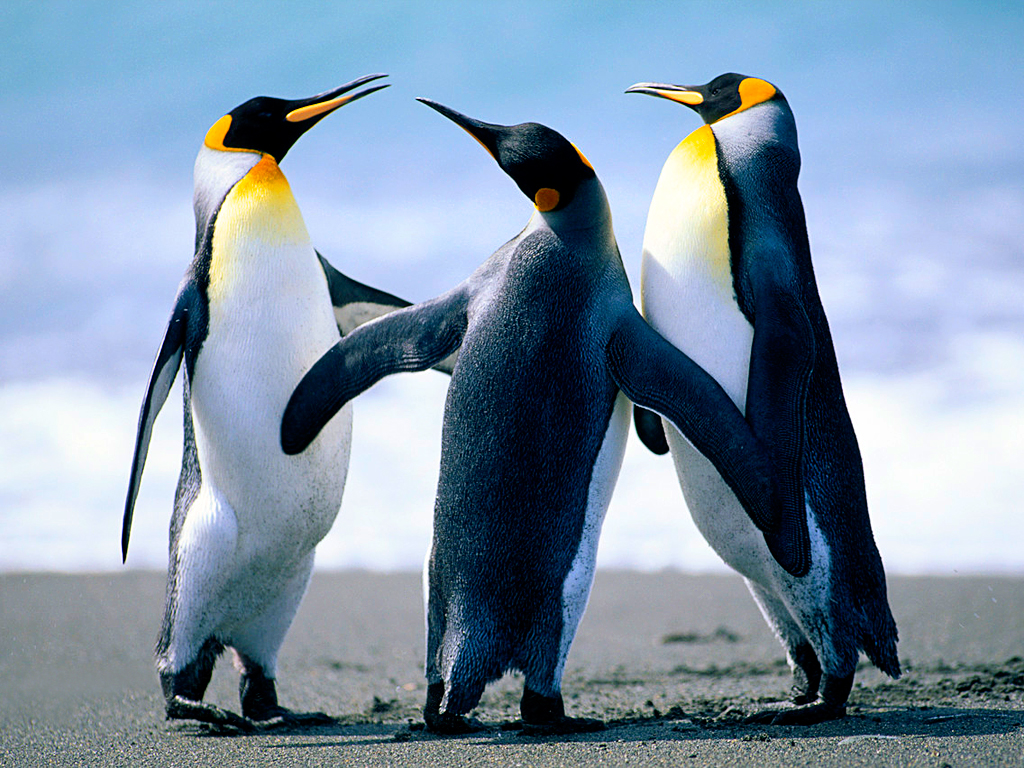
\includegraphics[scale=.50]{figures/Penguins.jpg}
\caption{TAMU figure - This is an example of a long figure title with a landscape figure.  Figure titles need to be single-spaced within and double spaced between in the list of figures.}
\label{fig:tamu-fig1-1}
\end{sidewaysfigure}
%%%%%%%%%%%%%%%%%%%%%%%%%%%%%%%%%%%%%%%%%%%%%%%%%%%%%%

More text here goes here.


Lorem ipsum dolor sit amet, consectetur adipiscing elit. Morbi augue urna, varius quis facilisis ac, imperdiet et nunc. Vestibulum ante ipsum primis in faucibus. 

\section{Testing the Top of the Page}
Maecenas accumsan lobortis dui fringilla suscipit. Quisque congue fringilla dui, sed eleifend sapien fringilla euismod. Pellentesque habitant morbi tristique senectus et netus et malesuada fames ac turpis egestas. Maecenas venenatis posuere magna quis tempus. Cras at leo massa, eu ultricies tellus. Nunc nec dictum augue. Cum sociis natoque penatibus et magnis dis parturient montes, nascetur ridiculus mus. Phasellus purus felis, mollis id scelerisque in, viverra in elit. Nulla iaculis ultrices justo, ac pharetra nisl rhoncus pulvinar. Duis vitae mauris velit, in congue massa.

Donec lectus orci, bibendum ut blandit dignissim, molestie non eros. Praesent aliquet feugiat dignissim. Morbi porttitor sollicitudin nisl, non mollis quam ultrices sit amet. Cras feugiat lacinia diam ut convallis. Nam nec varius ante. Nunc a ultrices felis. Quisque luctus sapien et ligula ornare quis consequat urna aliquet. Vestibulum vulputate lorem a tellus auctor id commodo risus sodales. Suspendisse quis tortor a felis molestie laoreet ut a nunc. Donec gravida sapien eget mauris condimentum lacinia. Proin eu purus libero. Nullam augue mi, vestibulum in convallis eu, adipiscing ac arcu. Donec nisi libero, egestas et molestie in, mollis quis ipsum. Sed gravida quam sit amet ante tempus rutrum non in mi. Cras viverra facilisis eros, id vestibulum sapien malesuada eget. Maecenas imperdiet luctus nisi vitae suscipit.



Aliquam erat volutpat. Integer ut mauris elit. Nam et lectus vel neque vehicula commodo. Integer at risus ligula. Fusce mollis mauris sed lorem aliquam bibendum porttitor tellus blandit. Curabitur enim nibh, accumsan eu elementum id, rutrum a ipsum. Vivamus ultricies, elit id ornare iaculis, metus justo posuere quam, sit amet bibendum arcu dolor a eros. Sed in nisl nibh. Aenean egestas est ut tortor volutpat vehicula. Maecenas aliquet placerat nunc hendrerit dictum. In et nisi massa. Pellentesque luctus, sapien quis dignissim vulputate, sapien libero bibendum velit, vitae auctor ipsum nulla at augue. Nulla ac eros vitae tortor elementum vehicula.

Morbi tristique egestas placerat. Cras faucibus eleifend porta. Class aptent taciti sociosqu ad litora torquent per conubia nostra, per inceptos himenaeos. Ut a pellentesque neque. Donec sollicitudin metus varius nulla egestas laoreet. Duis non mauris ut nunc adipiscing volutpat. Nam vitae est sed turpis tristique varius. 

\subsection{This is a Very Long Subsection Title This is a Very Long Subsection Title}

More text
\subsection{Subsection}

Subsection text

\section{Another Section}

Section text

%%%%%%%%%%%%%%%%%%%%%%%%%%%%%%%%%%%%%%%%%%%%%%%%%%%
%
%  New template code for TAMU Theses and Dissertations starting Fall 2012.  
%  For more info about this template or the 
%  TAMU LaTeX User's Group, see http://www.howdy.me/.
%
%  Author: Wendy Lynn Turner 
%	 Version 1.0 
%  Last updated 8/5/2012
%
%%%%%%%%%%%%%%%%%%%%%%%%%%%%%%%%%%%%%%%%%%%%%%%%%%%

%%%%%%%%%%%%%%%%%%%%%%%%%%%%%%%%%%%%%%%%%%%%%%%%%%%%%%%%%%%%%%%%%%%%%%
%%                           SECTION I
%%%%%%%%%%%%%%%%%%%%%%%%%%%%%%%%%%%%%%%%%%%%%%%%%%%%%%%%%%%%%%%%%%%%%
%
\chapter{\uppercase {Hyperbolic scalar and system of equations:}}
%
In this chapter, some key properties of the hyperbolic system of equations are recalled. The objective is to introduce the reader to the notion of shock, weak solution and entropy minimum principle by studying a simple hyperbolic scalar equation through a linear progression. First, the mathematical properties of the hyperbolic scalar equation are studied and include the derivation of the eigenvalue and the characteristic equation. Then, it is explained how shock are formed which will bring us to show that the solution is non-unique. The reader will be introduced to the notion of weak solution. Lastly, it will be explained how the entropy condition is used to ensure uniqueness of the solution and more importantly, ensure convergence of the numerical solution to the physical one. In the last section of this chapter, the notions introduced for the hyperbolic scalar equation are generalized to systems of equation.
%%%%%%%%%%%%%%%%%%%%
\section{Hyperbolic scalar equations:}
%%%%%%%%%%%%%%%%%%%%
The study of a hyperbolic scalar equation is detailed in order to provide the reader with a better understanding of its mathematical properties that are useful to the comprehension of shock formation among others.
%=============================
\subsection{Eigenvalue and characteristic curves:}\label{sec:mat_ppr}
%=============================
For academic purpose, we consider a simple hyperbolic scalar equation with initial conditions to form what is called an \emph{Initial Boundary Value Problem} (IBVP) as shown in \eqt{eq:ivp_sct1b}. We define a computational domain $\Omega$ of dimension $d$, bounded by the boundary $\Gamma$ of dimension $d-1$. Each variable is assumed to be a function of space, $\vec{r} \in R^d$, and time, $t \in R_+$.
%
\begin{equation}\label{eq:ivp_sct1b}
\left\{
\begin{array}{l}
\partial_t u(\vec{r},t) + \div ( f(u) \vec{n} ) = 0 \text{, } \left( \vec{r}, t \right) \in R^d \times R_+  \nonumber \\
u(\vec{r},0) = u( \vec{r}_0) 
\end{array}
\right.
\end{equation}
%
where $u$ and $f(u)$ are the solution and the inviscid flux, respectively. The inviscid flux $f(u)$ is assumed to be a differential function of the solution $u$. Two definitions of the inviscid flux will be considered in this chapter in order to illustrate the differences between linear and non-linear hyperbolic scalar systems: a linear flux $\vec{f}_1$ and a non-linear flux $\vec{f}_2$, as follows:
%
\begin{subequations}\label{eq:ivp2_sct1b}
%
\begin{equation}\label{eq:trans_sct1b}
\partial_t u(\vec{r},t) + \div \vec{f}_1(u) = \partial_t u(\vec{r},t) + \div \left( au \right) = 0
\end{equation}
%
\begin{equation}\label{eq:burger_sct1b}
\partial_t u(\vec{r},t) + \div \vec{f}_2(u) = \partial_t u(\vec{r},t) + \div \left( \frac{u^2}{2} \right) = 0
\end{equation}
%
\end{subequations}
%
\eqt{eq:trans_sct1b} and \eqt{eq:burger_sct1b} are respectively known as the transport and Burger's equations. They have been widely studied in the literature and are well understood (REFS). 

The eigenvalue, $\lambda$, of the hyperbolic equation is obtained by looking at the derivative of the inviscid flux, $f(u)$, with respect to the solution $u$, and corresponds to the wave propagation speed. When considering the fluxes $f_1$ and $f_2$, it is found that their eigenvalues are $\lambda_1 = a$ and $\lambda_2 = u$, respectively. For the linear advection equation, the wave speed is a constant through the computational domain. On the other hand, the wave speed is a function of space and time since equal to the solution itself, for the Burger's equation.

Once the eigenvalues are determined, the next step consists of deriving the characteristic equation and the characteristic curves. For implicitly purpose, we limit ourself to the $x-t$ plane. Under this assumption, characteristic curves are defined as curves $x = x(t)$ in the plane $x-t$ along with the PDE becomes an ODE \cite{Toro}. To determine the characteristic curves, \eqt{eq:ivp_sct1b} is recast as a function of the eigenvalue, $\lambda$, by using the chain rule as shown in 
%
\begin{eqnarray}\label{eq:ivp3_sct1b}
&&\partial_t u(\vec{r},t) + \frac{df}{du}\partial_x u = 0 \nonumber\\
&&\partial_t u(\vec{r},t) + \lambda \partial_x u = 0 \nonumber \\
&&\partial_t u(\vec{r},t) + \frac{dx}{dt} \partial_x u = 0 \text{ along } \frac{dx}{dt} = f'(u) = \lambda 
\end{eqnarray}
%
\eqt{eq:ivp3_sct1b} represents the rate of change of the solution $u$ along the curve $\frac{dx}{dt} = f'(u) = \lambda$. As a results, it tells us that the solution $u$ is constant along the curve $\frac{dx}{dt} = \lambda$ since its rate of change is zero. The eigenvalue is the slope of characteristic curve and is referred to as the characteristic speed. 
%For the linear advection equation, the characteristic speed is constant and equal to $a$, whereas it is a function of space and time for Burger's equation since equal to the solution itself. 
For a given characteristic curve, the characteristic speed is a constant, since the solution $u$ is constant as well, and given by the initial condition, $f'(u)=f'(u_0)$ which allows us to integrate in order to obtain an analytical expression:
%
\begin{eqnarray}\label{eq:ivp4_sct1b}
\frac{dx}{dt} &=& a \nonumber \\
\Leftrightarrow x(t) &=& x_0 + f'(u_0)t
\end{eqnarray}
%
where we set $x(t=0) = x_0$ that can be seen as the initial position of a particle traveling along the characteristic curve. It is current to represent the characteristic curves in a $t-x$ plane and example will be given for the linear advection and Burger's equation. \eqt{eq:ivp4_sct1b} informs us on the position $x$ of a particle of initial solution $u_0$ for each time $t$. Now, assuming that the initial value of the solution is $u_0(x_0)$ along the characteristic curve given by \eqt{eq:ivp4_sct1b} and passing through the point $x_0$, the solution $u(x,t)$ at position $x$ and time $t$ can be expressed as follows:
%
\begin{equation}\label{eq:ivp5_sct1b}
u(x,t) = u_0(x_0) = u_0(x - f'(u_0)t)
\end{equation}
%
\label{eq:ivp5_sct1b} can be seen as an analytical solution of the hyperbolic scalar equation (\eqt{eq:ivp_sct1b}). It is also understood that the derivative of the flux that corresponds to the eigenvalue of the system, has profound consequence on the behavior of the solution as explained in \sect{sec:shock_form}. 
%=============================
\subsection{Formation of shocks}\label{sec:shock_form}
%=============================
Hyperbolic scalar equations are known to develop shocks even from a smooth initial profile. This section aims at detailing how shocks form based on the mathematical properties introduced in \sect{sec:mat_ppr} and the two examples of \eqt{eq:trans_sct1b} and \eqt{eq:burger_sct1b}, i.e., the $1$-D linear advection and Burger's equations.\\

When considering the linear advection equation recalled in \eqt{eq:trans_sct1b} with the flux $f_1(u) = au$, the eigenvalue is found equal to $\lambda_1=a$ and constant. Thus, the slope of the characteristic curve remains constant and each particle travels at the same velocity through the computational domain. In other word, the initial profile of the solution is simply translated at speed $a$ to the right if $a \geq 0$ and to the left if $a \leq 0$. Obviously, if $a=0$, the flux is also null and the solution remains static. A representation of the characteristic curve for the linear advection equation, \eqt{eq:trans_sct1b}, is given in (FIGURE) in a $t-x$ plane: all of the characteristic curves are parallel since the eigenvalue is constant.

In the case of Burger's equation, the eigenvalue is, once again, obtained by computing the derivative of the flux $f_2(u) = u^2/2$, to obtain $\lambda_2 = u$. The slope of the characteristic curves is a function of the initial profile of the solution which requires the study of two distinct cases: a constant initial solution and a non-constant initial solution. In the former case, the slope of the characteristic is constant which is the identical case to the linear advection equation. In the later case, the characteristic curve will not have the same slope and may intersect. When two characteristic curves intersect, it means that at a given time and position, two values of the solution are allowed (each characteristic curve carries a different initial values of the solution): the solution displays an infinite gradient also called shock wave and can eventually leads to breaking wave type solution as shown in FIGURE. The time the shock occurs at can be analytically determined. Let consider a non-linear flux $f(u)$ and two characteristic curves originating from the position $x_0$ and $x_0+dx$ and carrying the initial values $u_0(x_0)$ and $u_0(x_0+dx)$, respectively. The characteristic curves are:
%
\begin{eqnarray}\label{eq:cc1_sct1b}
&&x_1 = x_0 + f'(u_0(x_0)) t \nonumber \\ 
&&x_2 = (x_0 + dx) + f'(u_0(x_0+dx)) t \nonumber 
\end{eqnarray}
%
Let now assume that the characteristic curves intersect at time $\tau_{shock}$, which implies $x_1 = x_2$. $\tau_{shock}$ is often referred to as the breaking time. Using \eqt{eq:cc1_sct1b}, an expression for $\tau_{shock}$ can be derived as follows: 
\begin{equation}
\tau_{shock} = \frac{-dx}{f'(u_0(x_0+dx))-f'(u_0(x_0))}
\end{equation} 
Taking the limit $dx \lim 0$ and using the definition of derivative, the above expression yields:
\begin{equation}\label{eq:cc2_sct1b}
\tau_{shock} = \frac{-1}{f''(u_0) u'_0} = \frac{-1}{f'(u_0)},
\end{equation} 
The trivial case $f''(u) = 0$ is ruled out since it was assumed a non-linear flux. However, let assume that the flux is linear. In that case, the second-order derivative is null and by taking the limit of \eqt{eq:cc2_sct1b}, it yields $\tau_{shock} \to \infty$ which means that a shock wave never forms. This result is consistent with conclusion made earlier in this section when studying the linear advection equation (\eqt{eq:trans_sct1b}). Going back to a non-linear flux, breaking first occurs where the derivative of the flux is negative and its absolute value is maximum.   \\
Knowing the breaking time $\tau_{shock}$ and position is not sufficient information to track a shock wave once it is formed. An useful information will be to derive an expression that provides us with the speed of the shock. One of the reason for deriving such expression is, to obtain an analytical solution that can be used for comparison against numerical solutions in order to assess their accuracy. To do so, we consider, one again, a general $1$-D hyperbolic scalar equation for simplicity as shown in 
%
\begin{equation}\label{eq:rh_sct1b}
\partial_t u(x,t) + \partial_x f(u(x,t)) = 0
\end{equation}
%
We assume that the position of the shock is given by a function of time denoted by $s(t)$ and that the associated speed is $S = \frac{ds}{dt}$. At this particular position, the derivatives of the solution $u$ and the flux $f(u)$ are not continuous. We also define a control volume $\left[ x_1; x_2 \right]$ that contains the shock wave so that $x_1 \leq s(t) \leq x_2$. \eqt{eq:rh_sct1b} is integrated over the control volume as shown in \eqt{eq:rh2_sct1b}:
%
\begin{equation}\label{eq:rh2_sct1b}
\frac{d}{dt} \int_{x_1}^{s(t)} u(x,t) dx + \frac{d}{dt} \int_{s(t)}^{x_2} u(x,t) dx + f(x_2,t) - f(x_1,t) = 0
\end{equation}
% 
The first two integrals can be recast by using the following chain rule:
%
\begin{equation}\label{eq:rh3_sct1b}
\frac{d}{dt} \int_{y_1(t)}^{y_2(t)} g(y,t) dy =  \int_{y_1(t)}^{y_2(t)} g(y,t) dy + g(y_2,t) \frac{d y_2(t)}{dt} - g(y_1,t) \frac{d y_1(t)}{dt},
\end{equation}
% 
which yields by noticing that $x_1$ and $x_2$ are not a function of time:
%
\begin{equation}\label{eq:rh4_sct1b}
\int_{x_1}^{s(t)} \partial_t u(x,t) dx - \int_{s(t)}^{x_2} \partial_t u(x,t) dx + \left( u(s^-(t)) - u(s^+(t)) \right) S + f(x_2,t) - f(x_1,t) = 0
\end{equation}
%
where $u(s^-(t),t)$ and $u(s^+(t),t)$ are the values of the solution $u$ before and after the shock, respectively. We now assume that the $x_1$ and $x_2$ approach the shock position $s(t)$ from the left and right, respectively, and that $\partial_t u$ is bounded, the integrals vanish to yield the following expression for the speed of shock $S$:
%
\begin{equation}\label{eq:rh5_sct1b}
S = \frac{f(x_2,t) - f(x_1,t)}{u(s^-(t)) - u(s^+(t))} = \frac{\Delta f}{\Delta u}
\end{equation}
%
The above expression computing the speed of shock (\eqt{eq:rh5_sct1b}) is known as the Rankine-Hugoniot jump condition. The hyperbolic scalar equation given \eqt{eq:rh_sct1b} is only valid in smooth parts of the solution, and thus, require the use of the Rankine-Hugoniot jump condition in order to solve for the shock region.   
%its speed can be determined by the Rankine-Hugoniot condition
%However, along the characteristic curves, the solution remains constant which allows us to integrate to obtain an analytical expression for the characteristic curve. For the purpose of plotting the characteristic curves, we assume a computational domain of length one and that the initial condition for the solution is of the form $u(x_0) = \sin (\pi x)$. With such initial condition, the slope of the characteristic curve is no longer constant but vary both in time and space. As a result, some of the characteristic curves will intersect  
\begin{itemize}
\item hyperbolic scalar equations are known to produce shocks even with smooth initial conditions.
\item explain how shocks can form with characteristic equations.
\item talk about diffusion equation that does not produce shocks -> same equation but with diffusion term that smoothes out shocks. Solution is unique and smooth.
\item idea is to add diffusion to the hyperbolic equation in order to control the shock.
\end{itemize}
%=============================
\subsection{Weak solution:}
%=============================
introduce the notion of weak solution and non-uniqueness of the weak solution.
%===============================
\subsection{Entropy minimum principle:}
%===============================
%===============================
\subsection{Entropy viscosity method for the multi-D Burger equation:}
%===============================
Condition for uniqueness of the solution. Show an example of the derivation for Burger's equations.
%%%%%%%%%%%%%%%%%%%%%
\section{Hyperbolic system of equations:}
%%%%%%%%%%%%%%%%%%%%%
\begin{itemize}
\item hyperbolic system of equations can also produce shocks.
\item same treatment as scalar equations.
\end{itemize}
%%%%%%%%%%%%%%%%%%%%%
\section{Remarks concerning the application of the entropy viscosity method to hyperbolic system of equations:}
%%%%%%%%%%%%%%%%%%%%%
%%%%%%%%%%%%%%%%%%%%%%%%%%%%%%%%%%%%%%%%%%%%%%%%%%%
%
%  New template code for TAMU Theses and Dissertations starting Fall 2012.  
%  For more info about this template or the 
%  TAMU LaTeX User's Group, see http://www.howdy.me/.
%
%  Author: Wendy Lynn Turner 
%	 Version 1.0 
%  Last updated 8/5/2012
%
%%%%%%%%%%%%%%%%%%%%%%%%%%%%%%%%%%%%%%%%%%%%%%%%%%%

%%%%%%%%%%%%%%%%%%%%%%%%%%%%%%%%%%%%%%%%%%%%%%%%%%%%%%%%%%%%%%%%%%%%%%
%%                           SECTION I
%%%%%%%%%%%%%%%%%%%%%%%%%%%%%%%%%%%%%%%%%%%%%%%%%%%%%%%%%%%%%%%%%%%%%

\pagestyle{plain} % No headers, just page numbers
\pagenumbering{arabic} % Arabic numerals
\setcounter{page}{1}
%%%%%%%%%%%%%%%%%%%%%%%%%%%%%%%%%%%%%%%%%%%%%%%%%%%
%%%%%%%%%%%%%%%%%%%%%%%%%%%%%%%%%%%%%%%%%%%%%%%%%%%
\chapter{\uppercase {Discretization method and implementation details of the entropy viscosity method.}}
%%%%%%%%%%%%%%%%%%%%%%%%%%%%%%%%%%%%%%%%%%%%%%%%%%%
%%%%%%%%%%%%%%%%%%%%%%%%%%%%%%%%%%%%%%%%%%%%%%%%%%%
%==============================================================================
\section{Implementation of the entropy viscosity method (EVM) with continuous Galerkin finite element method:}
%==============================================================================
After describing the theoretical approach that leads to the derivation of the dissipative terms consistent with the entropy minimum principle and the definition of the viscosity coefficient, this section focuses on the implementation of the method: details are given on how to implement and compute the jump, the entropy residual and the dissipative terms, for instance. Most of the explanation given in this section can be applied to any schemes other than the Galerkin continuous finite element method. Special attention is required for the jump since their definition is scheme dependent. In this section, to explain the steps involved in the implementation of the EVM, we consider a on-uniform $2$-D mesh family $\Omega$. Each member of this family is called element, $e$, and the set of its faces is denoted by $\delta e = \left\{ \delta e_k \right\}$, where $k$ is the number of faces. To integrate the integral over each element $e$ and the boundaries $\delta e$, a quadrature rule, $Q = \left\{ q \right\}$ is used. For the purpose of this section, the EVM is applied to a hyperbolic system of $n$ equations given in \eqt{eq:system}. 
\begin{equation}\label{eq:system}2
\partial_t U(\vec{r},t) + \div F(U(\vec{r},t)) = \div G(U(\vec{r},t))
\end{equation}
where $U(\vec{r},t)$ and $F(U(\vec{r},t))$ are the vector conservative variables and the hyperbolic flux, respectively. The term $G(U(\vec{r},t))$ denotes the artificial dissipative terms that are assumed consistent with the entropy minimum principle \cite{jlg3}. All of the terms depend on space, $\vec{r}$ and time, $t$. It is also assumed that the eigenvalues, $\lambda = \left\{ \lambda_1, \lambda_2, \dots, \lambda_n \right\}$ are known. Lastly, the entropy residual is assumed to be of the following form:
\begin{equation}\label{eq:ent_residual_ex}
\partial_t S \left( U(\vec{r},t) \right) +  \grad \Phi \left( U(\vec{r},t) \right) \geq 0
\end{equation}
where $S$ is the entropy function and $\Phi$ is the associated entropy flux. \\ 
The first step in the implementation of the EVM is the integration of the dissipative terms over each element of the mesh. The continuous finite element approach consists of multiplying each term by a test function and then, integrating over the volume of each element. Since the dissipative terms are second-order spatial derivatives, an integration per part is performed leading to:
\begin{equation}
\div G(U(\vec{r},t)) \rightarrow \int_e \div G(U(\vec{r},t)) \phi(\vec{r}) = \int_{\delta e} G(U(\vec{r},t)) \phi(\vec{r}) - \int_e G(U(\vec{r},t)) \grad \phi(\vec{r}) \nonumber
\end{equation} 
where $\phi$ is a test function. Then, each integral is evaluating using the quadrature rule at the set of quadrature points $\vec{r}_q$:
\begin{equation}
\int_{\delta e} G(U(\vec{r},t)) \phi(\vec{r}) - \int_e G(U(\vec{r},t)) \grad \phi(\vec{r}) = \sum_{q,\delta e} G(U(\vec{r}_q,t)) \phi(\vec{r}_q) - \sum_{q,e} G(U(\vec{r}_q,t)) \grad \phi(\vec{r}_q) \nonumber
\end{equation}
The dissipative term $G(U(\vec{r},t))$ is function of the viscosity coefficient and the derivative of the conservative variables that need to be evaluated at the quadrature points. Obtaining the derivative values at the quadrature points with a continuous finite element discretization type is straightforward. On the other hand, computing the viscosity coefficient at the same quadrature points require a little bit more of computational work and is explained in the following. Details about the integral over the faces of each element will be given in the next paragraph.\\
The viscosity coefficient is not obtained by solving a PDE, but simply computed on the fly from the conservative variables. The definition of the viscosity coefficient $\mu(\vec{r},t)$ involves two other viscosity coefficients: a first-order viscosity coefficient $\mu_{max}(\vec{r},t)$ that is an upper bound, and a high-order viscosity coefficient often also called entropy viscosity coefficient that is denoted by $\mu_e(\vec{r},t)$. It is assumed that these viscosity coefficients are function of both space and time. The first-order viscosity coefficient is function of the local maximum eigenvalues and the mesh size $d$: $\mu_{max}(\vec{r},t) = \frac{d}{2} \max \lambda_k (\vec{r},t)$. For a shape regular mesh, the mesh size $d$ is expected to be finite. It is assumed that each element has its own finite mesh size denoted by $d_e$. For instance, when using libMesh (REF), a function can be called in order to get the mesh size or diameter of the cell under consideration. Obtaining the local maximum eigenvalue is self explanatory and has to be done for each quadrature point. At this point, in each element, $q$ different values of the first-order viscosity coefficient is available to us that we denote by the set: $\mu_{max}^e = \left\{ \mu_{max}(\vec{r}_q,t) \right\}$. \\
The high-order viscosity coefficient is trickier to compute since it involves the entropy residual and the jumps at the interface between cells.   
%The dissipative terms consist of second order spatial derivatives that are reduced to first order derivative by integrating per part after multiplying by the test function and integrating over the computational domain. An integral over the boundary of the computational domain also appears and raises the question of how to treat the dissipative terms on the boundary. It is often suitable to set the viscosity coefficients to zero on the boundary so that the boundary term coming from integrating per part the dissipative terms is also zero. Hyperbolic systems of equations alike the multi-D Euler equations, require particular treatment to compute the flux on the boundaries based on the study of the characteristic and the eigenvalues: the boundary terms of the dissipative terms could interfere with the hyperbolic flux and lead to the wrong value at the boundaries. The dissipative terms require to evaluate at each quadrature points of each cell the first-order spatial derivatives of one or multiple variables. With Galerkin finite element method, this task is easily done by using the derivative of the test functions. \\
%Once the dissipative terms are implemented, the viscosity coefficient has to be computed: the viscosity coefficient is evaluated on the fly from the entropy residual and the jumps. The viscosity coefficient requires to compute the first-order viscosity and the high-order viscosity coefficients at the quadrature points.
%%%%%%%%%%%%%%%%%%%%%%%%%%%%%%%%%%%%%%%%%%%%%%%%%%%
%
%  New template code for TAMU Theses and Dissertations starting Fall 2012.  
%  For more info about this template or the 
%  TAMU LaTeX User's Group, see http://www.howdy.me/.
%
%  Author: Wendy Lynn Turner 
%	 Version 1.0 
%  Last updated 8/5/2012
%
%%%%%%%%%%%%%%%%%%%%%%%%%%%%%%%%%%%%%%%%%%%%%%%%%%%

%%%%%%%%%%%%%%%%%%%%%%%%%%%%%%%%%%%%%%%%%%%%%%%%%%%%%%%%%%%%%%%%%%%%%%
%%                           SECTION III
%%%%%%%%%%%%%%%%%%%%%%%%%%%%%%%%%%%%%%%%%%%%%%%%%%%%%%%%%%%%%%%%%%%%%
%%%%%%%%%%%%%%%%%%%%%%%%%%%%%%%%%%%%%%%%%%%%%%%%%%%
%%%%%%%%%%%%%%%%%%%%%%%%%%%%%%%%%%%%%%%%%%%%%%%%%%%
\chapter{\uppercase {Application of the entropy viscosity method to the multi-D Burger's equation}}\label{chap:burger_chap3}
%%%%%%%%%%%%%%%%%%%%%%%%%%%%%%%%%%%%%%%%%%%%%%%%%%%
%%%%%%%%%%%%%%%%%%%%%%%%%%%%%%%%%%%%%%%%%%%%%%%%%%%
The multi-D Burger's equation is solved using the entropy viscosity method described in \sect{sec:evm_hyp_sc_sct1b}. The equation with the viscous regularization and the definition of the viscosity coefficients are recalled, and the treatment of the boundary condition in also explained in \sect{sec:burger_sct2b}. 1- and 2-D numerical results are presented in \sect{sec:num_sct2b}. The objective of this section is to present numerical results obtained with the entropy viscosity method for the simple hyperbolic scalar Burger's equation before dealing with hyperbolic system of equations. The multi-physics framework MOOSE \cite{Moose} was used to implement the multi-D Burger's equation. The code name is Badger.

%==============================================================================
\section{The multi-D Burger's equation}\label{sec:burger_sct2b}
%==============================================================================
We recall the multi-D Burger's equation (\eqt{eq:burger_eq_sct2b}) with the viscous regularization and the definition of the viscosity coefficient (\eqt{eq:burger_visc_sct2b}).
%
\begin{subequations}\label{eq:burger_sct2b}
%
\begin{equation}\label{eq:burger_eq_sct2b}
\partial_t u(\mbold{r},t) + \div \left( \frac{u(\mbold{r},t)^2}{2} \hat{\mbold{n}} \right) = \div \left( \mu(\mbold{r},t) \grad u(\mbold{r},t) \right)
\end{equation}
%
\begin{equation}\label{eq:burger_visc_sct2b}
\left\{
\begin{array}{l}
\mu(\mbold{r},t) = \min \left( \mu_{max} (\mbold{r},t),  \mu_e(\mbold{r},t)\right) \\
\mu_{max} (\mbold{r},t) = \frac{h}{2} | u(\mbold{r},t) | \\
\mu_e(\mbold{r},t) = h^2 \frac{\max\left( R_e(\mbold{r},t), J \right)}{|| s(\mbold{r},t) - \bar{s}(t) ||_\infty}
\end{array}
\right.
\end{equation}
%
\begin{equation}\label{eq:burger_res_sct2b}
\left\{
\begin{array}{l}
R_e(\mbold{r},t) = \partial_t s(\mbold{r},t) + \grad \left( u(\mbold{r},t) s(\mbold{r},t) \right) \\
J = \left[ u(\mbold{r},t) s(\mbold{r},t) \right]
\end{array}
\right.
\end{equation}
%
\end{subequations}
%
where $\hat{\mbold{n}}$ was previously defined in \sect{sec:mat_ppr_sct1b} as: $\hat{\mbold{n}} = \left(1, 0, 0 \right)$ in 1-D, $\hat{\mbold{n}} = \left(1, 1, 0 \right)$ in $2$-D and $\hat{\mbold{n}} = \left(1, 1, 1 \right)$ in $3$-D. The entropy function is denoted by $\eta$ and is taken equal to the convex function $\eta(\mbold{r},t) = u(\mbold{r},t)^2/2$ for the two examples presented in \sect{sec:num_sct2b}. The continuous Galerkin finite element method described in \chap{chap:disc_chap2} along with the second-order implicit itemporal integrator BDF2 are used to discretize \eqt{eq:burger_eq_sct2b}. Such discretization requires to compute the flux at the boundary of the computational domain \eqt{en:va_system_weak5}. Our implementation of the boundary condition for Burger's equation is based on the sign of the dot product $u(\mbold{r},t) \hat{\mbold{n}} \cdot \mbold{n} $ at the boundary, where $\mbold{n}$ is the outward normal to the boundary. For Burger's equation it was demonstrated in \sect{sec:mat_ppr_sct1b} that the eigenvalue is the solution itself $\lambda = u$. Being at the boundary, two cases have to be distinguished: 
\begin{itemize}
\item $u(\mbold{r},t) $ is negative: the wave enters the computational domain and thus, information needs to be supplied to the code. This boundary condition can be enforced either weakly or strongly. In the former case, the boundary value is specified in the input file, for instance, and used to compute the flux at the boundary. In the later case, the boundary value is still specified but strongly enforced with a Dirichlet boundary condition. This approach is valid for both implicit and explicit temporal integrators.
\item $u(\mbold{r},t) $ is positive: the wave exits the computational domain. The flux is computed with the value of the solution from the last Krylov iteration supplied by the temporal implicit solver. Because of the iterative process, the information normally carried by the waves is transmitted to the boundary. This approach is only valid with an implicit solver. When using an explicit solver, the solution at the new time on the boundary is obtained from the characteristic equation that is integrated over the first cell in.
\end{itemize}
% The above method for is a-dimensional and was used to obtain the numerical results presented in \eqt{sec:num_sct2b}.

%==============================================================================
\section{Numerical results}\label{sec:num_sct2b}
%==============================================================================
Two typical numerical tests are presented in order to illustrate the main features of the entropy viscosity method when applied to the multi-D Burger's equation.
%------------------------------------------------------------------------------------------------------
\subsection{1-D numerical result}\label{sec:1dnum_sct2b}
%------------------------------------------------------------------------------------------------------
We consider a 1-D computational domain of length $L=1$ $m$ discretized by an uniform mesh of $100$ elements. The initial condition consists of a smooth sinusoidal function $u(x,0) = \sin \left( 2 \pi x \right)$. The values at the left and right boundaries are set to zero and enforced by Dirichlet conditions. The numerical solution is run until $t=0.2$ $s$ with a $CFL$ of one. In order to investigate the effect of the entropy viscosity method onto the numerical solution, three tests are performed. In the first test, the numerical solution is run with first-order viscosity coefficient which implies $\mu(x,t) = \mu_{max}(x,t)$ at all point of the computational domain and for all time. Then, the same run is performed using the definition of $\mu(x,t)$ recalled in \eqt{eq:burger_visc_sct2b}. Lastly, the code is run without stabilization, $\mu(x,t) = 0$. The objective of running these three cases is to demonstrate the usefulness of the stabilization method and also to show the gain in accuracy when a high-order stabilization method is utilized. Numerical results are shown in \fig{fig:1d_burger_free} through \fig{fig:1d_burger_visc}. 
%
\begin{figure}[H]
        \centering
        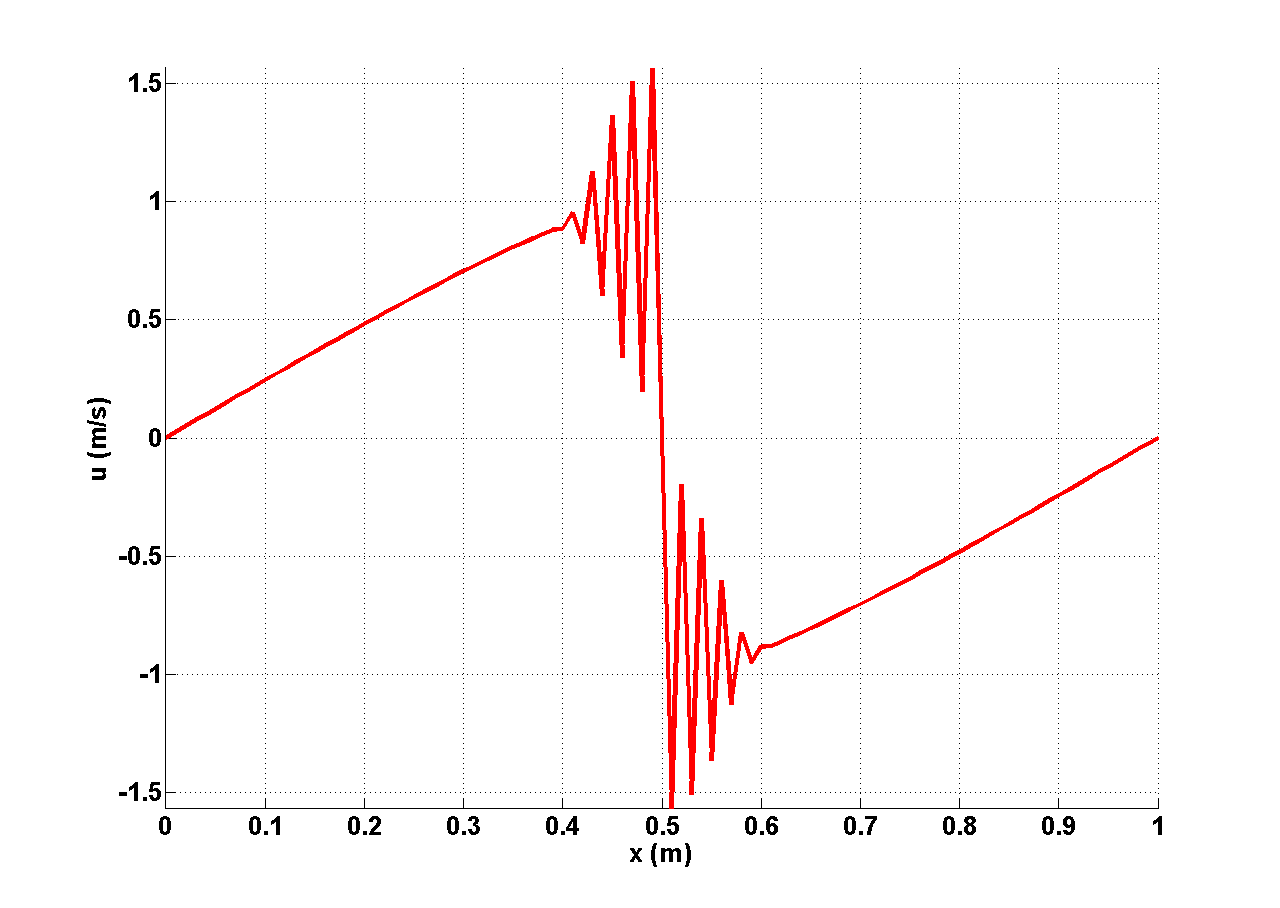
\includegraphics[width=0.8\textwidth]{figures/1D_sol_free.png}
        \caption{Solution profile without stabilization at $t=0.2$ $s$.}
        \label{fig:1d_burger_free}
\end{figure}
%
\begin{figure}[H]
        \centering
        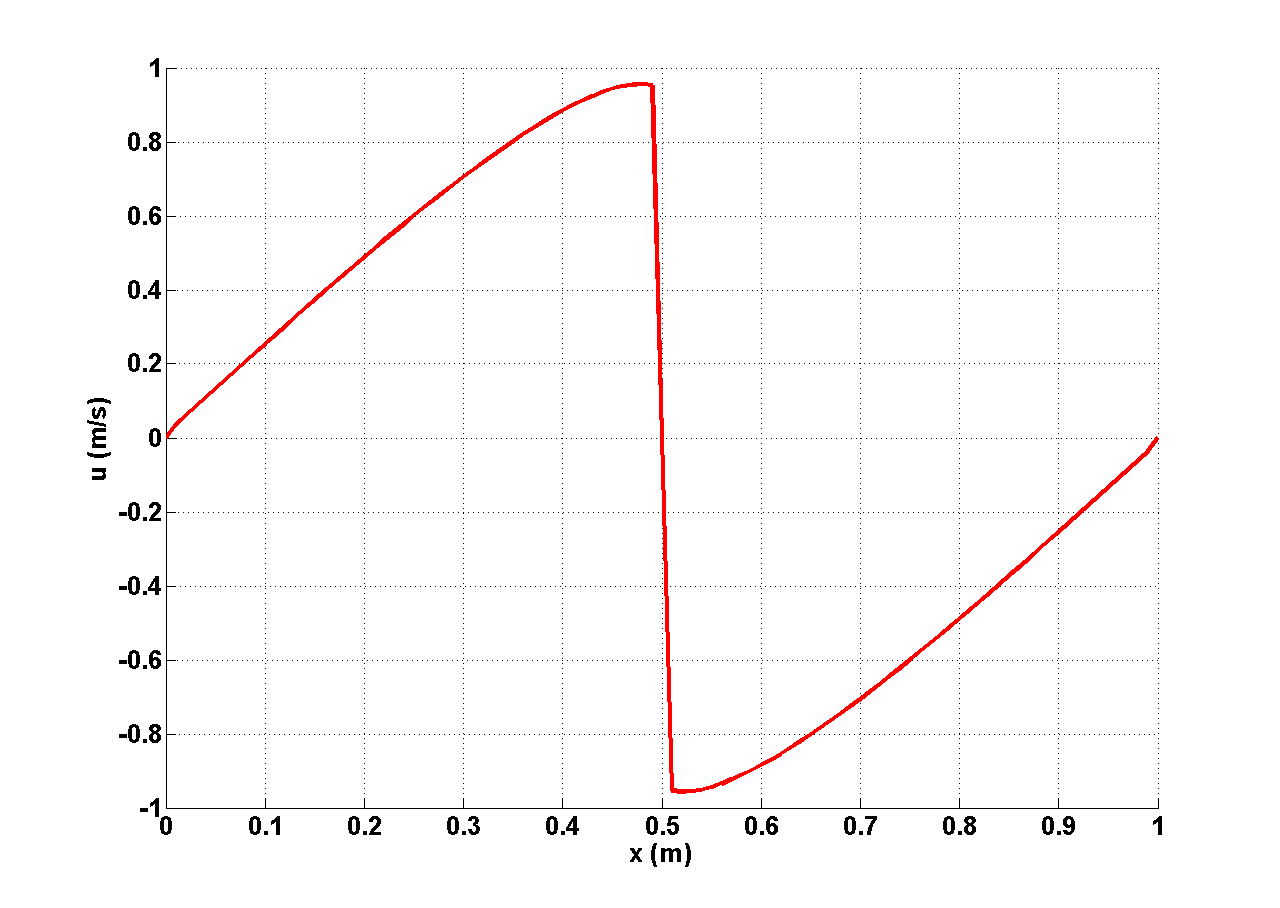
\includegraphics[width=0.8\textwidth]{figures/1D_sol_fo.png}
        \caption{Solution profile with first-order viscosity at $t=0.2$ $s$.}
        \label{fig:1d_burger_fo}
\end{figure}
        
\begin{figure}[H]
        \centering
        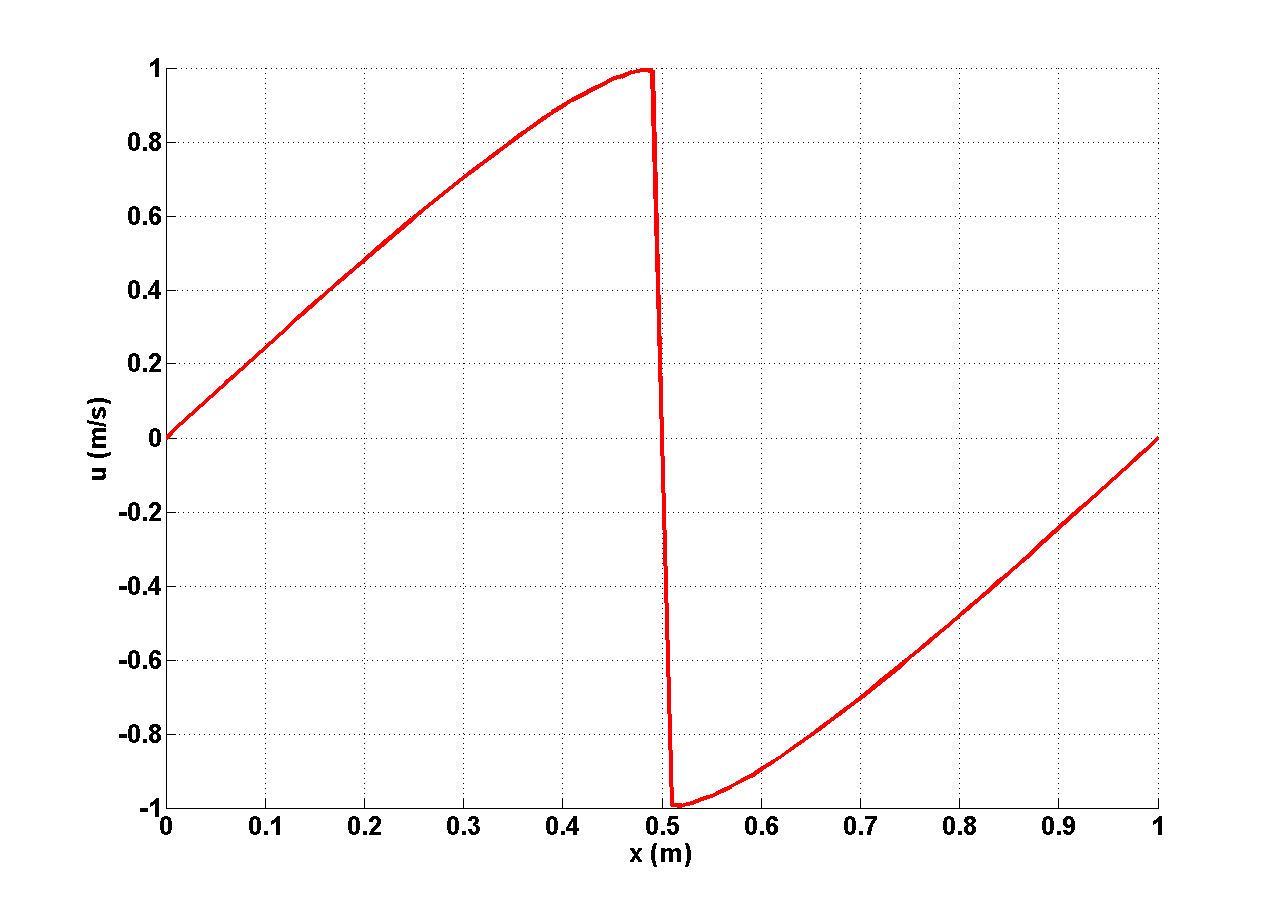
\includegraphics[width=0.8\textwidth]{figures/1D_sol_ev.png}
        \caption{Solution profile with the EVM at $t=0.2$ $s$.}
        \label{fig:1d_burger_ev}
\end{figure}
%       
\begin{figure}[H]
    \centering
    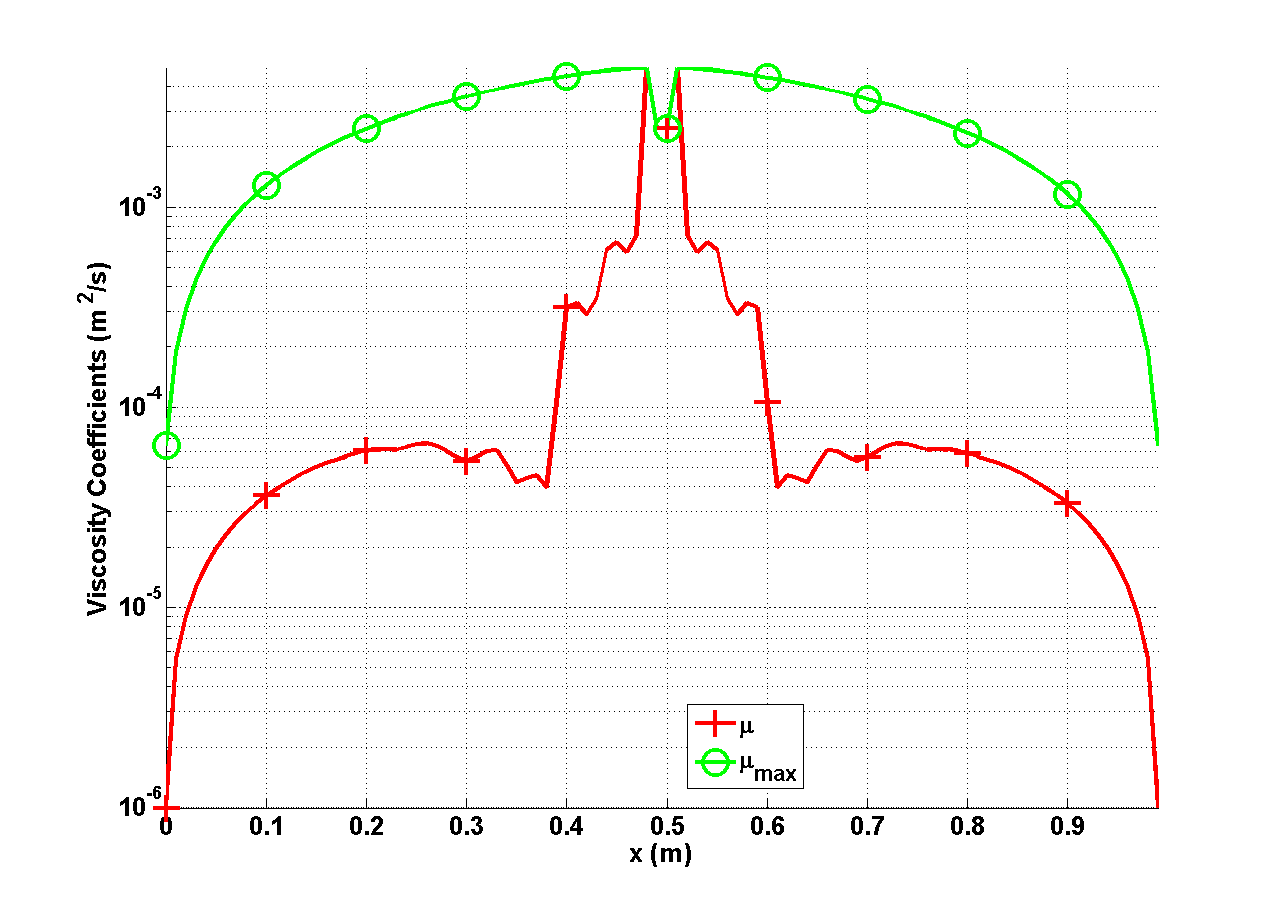
\includegraphics[width=0.8\textwidth]{figures/1D_visc.png}
    \caption{Viscosity coefficient profiles at $t=0.2$ $s$.}
    \label{fig:1d_burger_visc}
\end{figure}
%
In \fig{fig:1d_burger_free}, no stabilization  is used and numerical instabilities are observed in the shock region. When run with the over-dissipative first-order viscosity coefficient, the solution does not display any instabilities but the shock amplitude is smoothed as shown in \fig{fig:1d_burger_fo}. Lastly, the numerical solution obtained with the EVM in \fig{fig:1d_burger_ev} is very close to the exact solution: the shock amplitude is preserved and the solution is stable. The viscosity coefficients are shown in \fig{fig:1d_burger_visc} on a log-scale: the high-order viscosity coefficient $\mu_e$ is peaked in the shock region and is small anywhere else. This behavior is expected and corresponds to the theoretical approach detailed in \sect{sec:evm_hyp_sc_sct1b}. It was demonstrated in \cite{valentin} that high-order accuracy is preserved with the EVM when the solution is smooth (i.e. away from the shock region). It is also noticed in \fig{fig:1d_burger_visc} the difference of order of magnitude between the high- and first-order viscosity coefficients away from the shock region.
%------------------------------------------------------------------------------------------------------
\subsection{2-D Riemann problem}\label{sec:2dnum_sct2b}
%------------------------------------------------------------------------------------------------------
We now consider a typical 2-D benchmark problem known as Riemann problem. The computational domain consists of a $1 \times 1$ square and the following initial conditions are used:
%
\begin{equation}\label{eq:bg_2d_ic_sct2b}
u(\mbold{r},0) = u_0 = \left\{
\begin{array}{l}
+0.5 \text{ for } x \leq 0.5 \text{ and } y \leq 0.5 \\
+0.8 \text{ for } x \geq 0.5 \text{ and } y \leq 0.5 \\
-0.2 \text{ for } x \leq 0.5 \text{ and } y \geq 0.5 \\
-1. \text{ for } x \geq 0.5 \text{ and } y \geq 0.5
\end{array}
\nonumber
\right.
\end{equation}
%
An uniform mesh of $100 \times 100$ elements is used. The solution is run until $t=0.5$ $s$ with a $CFL$ of $0.5$. The numerical solution and the viscosity coefficient profiles are given next. 
%
\begin{figure}[H]
	\centering
	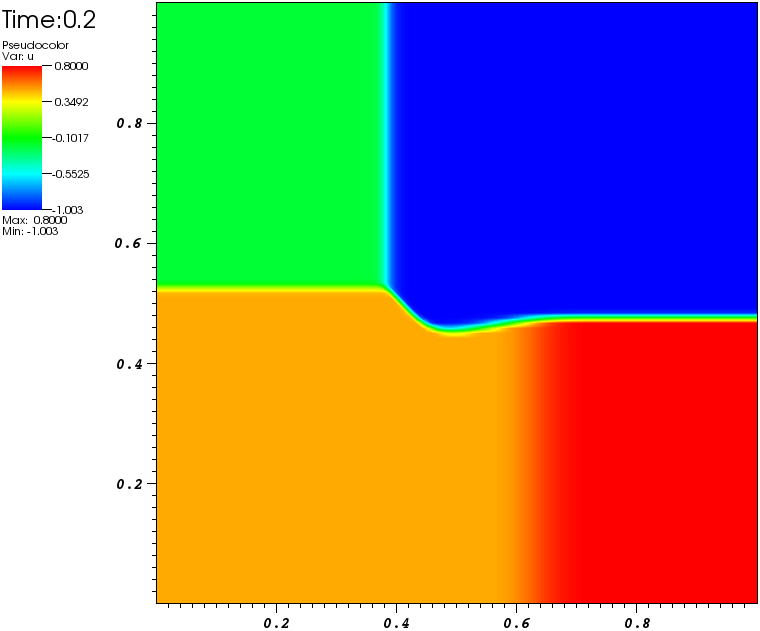
\includegraphics[width=\textwidth]{figures/Burger2D_sol_t0p2.png}
	\caption{Solution profile at $t=0.2$ $s$.}
	\label{fig:2d_burger_sol_t0p2}
\end{figure}
%
\begin{figure}[H]
	\centering
	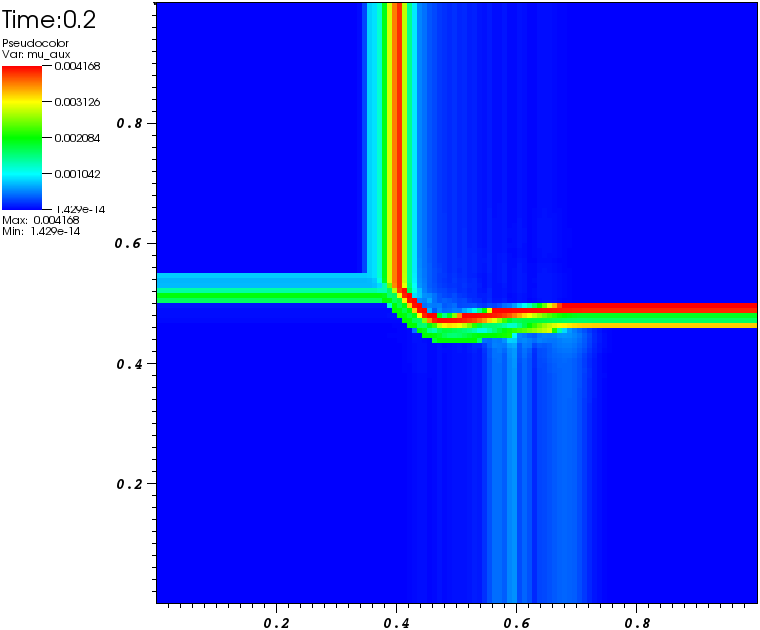
\includegraphics[width=\textwidth]{figures/Burger2D_visc_t0p2.png}
	\caption{Viscosity profile at $t=0.2$ $s$.}
	\label{fig:2d_burger_visc_t0p2}
\end{figure}
%
\begin{figure}[H]
	\centering
	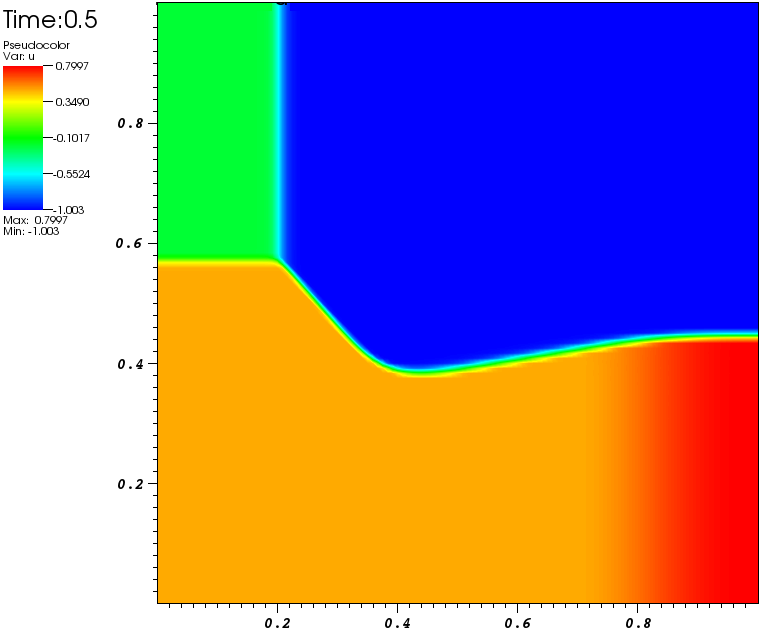
\includegraphics[width=\textwidth]{figures/Burger2D_sol_t0p5.png}
	\caption{Solution profile at $t=0.5$ $s$.}
	\label{fig:2d_burger_sol_t0p5}
\end{figure}
%
\begin{figure}[H]
	\centering
	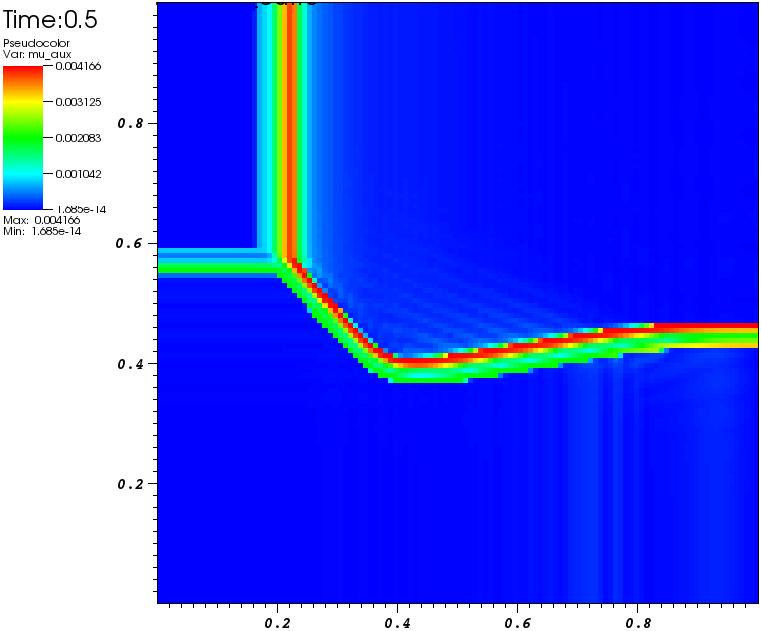
\includegraphics[width=\textwidth]{figures/Burger2D_visc_t0p5.png}
	\caption{Viscosity profile at $t=0.5$ $s$.}
	\label{fig:2d_burger_visc_t0p5}
\end{figure}
%
The numerical solution is plotted in \fig{fig:2d_burger_sol_t0p2} and \fig{fig:2d_burger_sol_t0p5} at $t=0.2$ and $t=0.5$ $s$, respectively. The numerical solution does not display any oscillations and the shocks are well resolved. The high-order viscosity coefficient is showed in \fig{fig:2d_burger_visc_t0p2} and \fig{fig:2d_burger_visc_t0p5}: the shock is well tracked by the EVM and sufficient dissipation is only added in the shock regions, where saturation to the first-order viscosity is achieved.\\

The above examples were simple illustrations of the capabilities of the EVM when applied to hyperbolic scalar equations. We now focus our attention to the application of the EVM to various hyperbolic systems of equations.
%%%%%%%%%%%%%%%%%%%%%%%%%%%%%%%%%%%%%%%%%%%%%%%%%%%
%
%  New template code for TAMU Theses and Dissertations starting Fall 2012.  
%  For more info about this template or the 
%  TAMU LaTeX User's Group, see http://www.howdy.me/.
%
%  Author: Wendy Lynn Turner 
%	 Version 1.0 
%  Last updated 8/5/2012
%
%%%%%%%%%%%%%%%%%%%%%%%%%%%%%%%%%%%%%%%%%%%%%%%%%%%

%%%%%%%%%%%%%%%%%%%%%%%%%%%%%%%%%%%%%%%%%%%%%%%%%%%%%%%%%%%%%%%%%%%%%%%
%%%                           SECTION II
%%%%%%%%%%%%%%%%%%%%%%%%%%%%%%%%%%%%%%%%%%%%%%%%%%%%%%%%%%%%%%%%%%%%%%

\chapter{\uppercase {Application of the entropy viscosity method to the multi-D Euler equations with variable area:}}
%%%%%%%%%%%%%%%%%%%%%%%%%%%%%%%%%%%%%%%%%%%%%%%%%%%%%%%%%%%%%
%%%%%%%%%%%%%%%%%%%%%%%%%%%%%%%%%%%%%%%%%%%%%%%%%%%%%%%%%%%%%
\section{Introduction} \label{sec:intro}
%%%%%%%%%%%%%%%%%%%%%%%%%%%%%%%%%%%%%%%%%%%%%%%%%%%%%%%%%%%%%%%%%%%%%%%%%%%%%%%%%%%%%%%%%%%%%%%%%%%%
%%%%%%%%%%%%%%%%%%%%%%%%%%%%%%%%%%%%%%%%%%%%%%%%%%%%%%%%%%%%%%%%%%%%%%%%%%%%%%%%%%%%%%%%%%%%%%%%%%%%
Over the past years an increasing interest raised for computational methods that can solve both compressible and incompressible flows. In engineering applications, there is often the need to solve for complex flows where a near incompressible regime or low Mach flow coexists with a supersonic flow domain. For example, such flow are encountered in aerodynamic in the study of airships. In the nuclear industry, flows are nearly the incompressible regime but compressible effects cannot be neglected because of the heat source and thus needs to be accurately resolved. \\
When solving the multi-D Euler equations for a wide range of Mach numbers, multiple problems have to address: stability, accuracy and acceleration of the convergence in the low Mach regime. Because of the hyperbolic nature of the equations, shocks can form during transonic and supersonic flows, and require the use of the numerical methods in order to stabilize the scheme and correctly resolve the discontinuities. The literature offers a wide range of stabilization methods: flux-limiter \cite{FluxLimiter, FluxLimiter2}, pressure-based viscosity method (\cite{PBV_book}), Lapidus method (\cite{Lapidus_paper, LMP, Lapidus_book}), and the entropy-viscosity method(\cite{jlg1, jlg2}) among others. These numerical methods are usually developed using simple equation of states and tested for transonic and supersonic flows where the disparity between the acoustic waves and the fluid speed is not large since the Mach number is of order one. This approach leads to a well-known accuracy problem in the low Mach regime where the fluid velocity is smaller that the speed of sound by multiple order of magnitude. The numerical dissipative terms become ill-scaled in the low Mach regime and lead to the wrong numerical solution by changing the nature of the equations solved. This behavior is well documented in the literature \cite{LowMach1, LowMach2, LowMach3} and often treated by performing a low Mach asymptotic study of the multi-D Euler equation. This method was originally used \cite{LowMach1} to show convergence of the compressible multi-D Euler equations to the incompressible ones. Thus, by using the same method, the effect of the dissipative terms in the low Mach regime, can be understood and, when needed, a fix is developed in order to ensure the convergence of the equations to the correct physical solution. This approach was used as a fixing method for multiple well known stabilization methods alike Roe scheme (\cite{Roe}) and SUPG \cite{LowMach3} while preserving the original stabilization properties of shocks.  \\
We propose, through this paper, to investigate how the entropy viscosity method, when applied to the multi-D Euler equations with variable area, behaves in the low Mach regime. This method was initially introduced by Guermond et al. to solve for the hyperbolic systems and has shown good results when used for solving the multi-D Euler equations with various discretization schemes. More importantly, it is simple to implement, can be used with unstructured grids,  and its dissipative terms are consistent with the entropy minimum principle and proven valid for any equation of state under certain conditions \cite{jlg}. \\
This paper is organized as follows: in \sect{sec:entro_visc} the current definition of the entropy viscosity method is recalled, and inconsistency with the low Mach regime are pointed out. Since our interest is in the variable area version of the multi-D Euler equation, the reader is guided trough the steps leading to the derivation of the dissipative terms on the model of \cite{jlg}. Then in \sect{sec:extension}, a new definition of the viscosity coefficient is introduced and derived from a low Mach asymptotic study. After detailing the spatial and temporal discretization method in \sect{sec:solution_tech}, $1$- and $2$-D numerical results are presented in \sect{sec:results} for a wide range of Mach numbers: low Mach flow over a cylinder and a circular bump, and supersonic flow in a compression corner \cite{CompressionCorner}. Convergence studies are performed in $1$-D, in order to demonstrate the accuracy of the solution. \\
For purpose of clarity, the multi-D Euler equations with variable area are recalled in \eqt{eq:euler_eq} and the corresponding variables are defined:
\begin{equation}
\label{eq:euler_eq}
\left\{ 
\begin{array}{lll}
\partial_t \left( \rho A\right) + \div \left( \rho \vec{u} A\right) = 0\\
\partial_t \left( \rho \vec{u} A\right) + \div \left[ \left( \rho \vec{u} \otimes \vec{u} + P \mathbf{I} \right) A \right] = P \grad A\\
\partial_t \left( \rho E A\right) + \div \left[ \vec{u} \left( \rho E + P \right) A\right] = 0 \\
P = P\left( \rho, e \right)
\end{array}
\right.
\end{equation}
where $\rho$, $\rho \vec{u}$ and $\rho E$ are the density, the momentum and the total energy, respectively, and will be referred to as the conservative variables. The pressure $P$ is computed with an equation of state expressed in function of the density $\rho$ and the specific internal energy $e$. The tensor product $\vec{a} \otimes \vec{b}$ is taken with the following convention: $(\vec{a} \otimes \vec{b})_{i,j} = a_i b_j$. Lastly, the terms $\partial_t$, $\grad$, $\div$ and $\mathbf{I}$ denote the temporal derivative, the gradient and divergent operators, and the identity tensor, respectively. The variable area $A$ is assumed spatial dependent.
%%%%%%%%%%%%%%%%%%%%%%%%%%%%%%%%%%%%%%%%%%%%%%%%%%%%%%%%%%%%%%%%%%%%%%%%%%%%%%%%%%%%%%%%%%%%%%%%%%%%
%%%%%%%%%%%%%%%%%%%%%%%%%%%%%%%%%%%%%%%%%%%%%%%%%%%%%%%%%%%%%%%%%%%%%%%%%%%%%%%%%%%%%%%%%%%%%%%%%%%%
\section{The Entropy Viscosity Method} \label{sec:entro_visc}
%%%%%%%%%%%%%%%%%%%%%%%%%%%%%%%%%%%%%%%%%%%%%%%%%%%%%%%%%%%%%%%%%%%%%%%%%%%%%%%%%%%%%%%%%%%%%%%%%%%%
%%%%%%%%%%%%%%%%%%%%%%%%%%%%%%%%%%%%%%%%%%%%%%%%%%%%%%%%%%%%%%%%%%%%%%%%%%%%%%%%%%%%%%%%%%%%%%%%%%%%
%===================================================================================================
\subsection{Background} \label{sec:background}
%===================================================================================================
In this section, the entropy-based viscosity method \cite{jlg1, jlg2, jlg3} is recalled for the multi-D Euler equations (with constant area $A$) \cite{valentin}. The entropy-based viscosity method consists of adding dissipative terms, with a viscosity coefficient modulated by the entropy production which allows high-order accuracy when the solution is smooth. Thus, two questions arise: (i) how are the viscosity dissipative terms derived and (ii) how to numerically compute the entropy production. Answers to the first question can be found in \cite{jlg} by Guermond et al., that details the proof leading to the derivation of the artificial dissipative terms (\eqt{eq:euler_visc}) consistent with the entropy minimum principle theorem. The viscous regularization obtained is valid for any equation of state as long as the opposite of the physical entropy function, $s$, is convex with respect to the internal energy $e$ and the specific volume $1/\rho$. As for the entropy production, it is locally evaluated by computing the local entropy residual $D_e(\vec{x},t)$ defined in \eqt{eq:ent_visc_coeff}, that is known to be peaked in shocks \cite{Toro}.
\begin{equation}
\label{eq:euler_visc}
\left\{ 
\begin{array}{lll}
\partial_t \left( \rho \right) + \div \left( \rho \vec{u} \right) = \div \left( \kappa \grad \rho \right) \\
\partial_t \left( \rho \vec{u} \right) + \div \left( \rho \vec{u} \otimes \vec{u} + P \mathbf{I} \right) = \div \left( \mu \rho \grad^s \vec{u}  + \kappa \vec{u} \otimes \grad \rho \right)  \\
\partial_t \left( \rho E \right) + \div \left[ \vec{u} \left( \rho E + P \right) \right] = \div \left( \kappa \grad \left( \rho e \right) + \frac{1}{2}|| \vec{u} ||^2 \kappa \grad \rho +  \rho \mu \vec{u} \grad \vec{u}  \right) \\
P = P\left( \rho, e \right)
\end{array}
\right.
\end{equation}
where $\kappa$ and $\mu$ are local positive viscosity coefficients. $\grad^s \vec{u}$ denotes the symmetric gradient operator that guarantees the method to be rotational invariant \cite{jlg}.\\
In the current version of the method, $\kappa$ and $\mu$ are set equal, so that the above viscous regularization (\eqt{eq:euler_visc}) is equivalent to the parabolic regularization \cite{Parabolic} when considering the $1$-D form of the equation. The current definition includes a first-order viscosity coefficient referred to with the subscript $max$, and a high-order viscosity coefficient referred to with the subscript $e$. The first-order viscosity coefficients $\mu_{max}$ and $\kappa_{max}$ are proportional to the local largest eigenvalue $|| \vec{u} || + c $ and equivalent to an upwind-scheme (see \eqt{eq:fo}), when used, which is known to be over-dissipative and monotone \cite{Toro}: 
\begin{equation}
\label{eq:fo}
\mu_{max}(\vec{r}, t) = \kappa_{max}(\vec{r}, t) = \frac{h}{2} \left( || \vec{u} || + c \right),
\end{equation}
where $h$ is defined as the ratio of the grid size to the polynomial order of the test functions used. \\
The second-order viscosity coefficients $\kappa_e$ and $\mu_e$ are set proportional to the entropy production that is evaluated by computing the local entropy residual $D_e$. It also includes the interfacial jump of the entropy flux $J$ that will allow to detect any discontinuities other than shocks:
\begin{equation}
\label{eq:ent_visc_coeff}
\mu_e(\vec{r},t) = \kappa_e(\vec{r},t) = h^2 \frac{\max\left( | D_e(\vec{r},t) |, J \right)}{|| s - \bar{s} ||_{\infty}} \text{ with } D_e(\vec{r}, t) = \partial_t s + \vec{u} \cdot \grad s
\end{equation}
where $|| \cdot ||_{\infty}$ and $\bar{\cdot}$ denote the infinite norm operator and the average operator over the entire computational domain, respectively. The definition of the jump $J$ is discretization-dependent and examples of definition can be found in \cite{valentin} for DGFEM. The denominator $|| s - \bar{s} ||_{\infty}$ is used for dimensionality purposes and should not be of the same order as $h$, on penalty of loosing the high-order accuracy. Currently, there are no theoretical justification for choosing the denominator. \\
The definition of the viscosity coefficients $\mu$ and $\kappa$ is function of the first- and second-order viscosity coefficients as follows:
\begin{equation}
\mu(\vec{r},t) = \min\left( \mu_e(\vec{r},t), \mu_{max}(\vec{r},t) \right) \text{ and } \kappa(\vec{r},t) = \min\left( \kappa_e(\vec{r},t), \kappa_{max}(\vec{r},t) \right).
\end{equation}
This definition allows the following properties.
In shock regions, the second-order viscosity coefficient experiences a peak because of entropy production, and thus, saturates to the first-order viscosity that is known to be over-dissipative and will smooth out oscillations. Anywhere else, the entropy production being small, the viscosity coefficients $\mu$ and $\kappa$ are of order $h^2$.\\
Using the above definition of the entropy-based viscosity method, high-order accuracy was demonstrated and excellent results were obtained with 1-D Sod shock tubes and various 2-D tests \cite{jlg1, jlg2, valentin}.
%===================================================================================================
\subsection{Issues in the Low-Mach Regime} 
%===================================================================================================
In the Low-Mach Regime, the flow is known to be isentropic resulting in very little entropy production. Since the entropy viscosity method is directly based on the evaluation of the local entropy production, it will be interested to study how the entropy viscosity coefficients $\mu$ and $\kappa$ scale in the low Mach regime. Mathematically, it means that the entropy residual $D_e$ will be very small, so will be the denominator $|| s - \bar{s} ||_{\infty}$, thus making the ratio, used in the definition of the viscosity coefficients \eqt{eq:ent_visc_coeff}, undetermined.  Therefore, the current definition of the viscosity coefficients seems unadapted to subsonic flow and could lead to ill-scaled dissipative terms. A solution would be to recast the entropy residual as a function of other variables in order to have more freedom in the choice of the normalization parameter. 
With this approach, the viscosity coefficients are still defined proportional to the entropy residual that is a good indicator of the flow type (subsonic, transonic and supersonic flow). Plus, a different normalization parameter could be chosen, based on a low Mach asymptotic study so that the viscosity coefficients are well-scaled in the low Mach asymptotic limit (see \sect{sec:extension}).
%The idea is to still define the viscosity coefficient proportional to the entropy residual since it is a good indicator of the flow type (subsonic or supersonic).
%===================================================================================================
\subsection{The dissipative-terms for the multi-D Euler equations with variable area} 
%===================================================================================================
One of the focus of this paper is to investigate the application of the entropy viscosity method to the multi-D Euler equations with variable area. The variable area version of the Euler equations is mostly used in $1$-D and $2$-D for obvious reasons, and differs from \eqt{eq:euler_eq} by the momentum equation as shown in \eqt{eq:euler_variable_A}, that contains a non-conservative term proportional to the area gradient. For the purpose of this paper, the variable area is assumed to be a smooth function and only spatial dependent. An example can be found in \cite{SEM} where a fluid flows through a $1$-D convergent-divergent nozzle and reaches a steady-state solution.
\begin{equation}
\label{eq:euler_variable_A}
\left\{ 
\begin{array}{lll}
\partial_t \left( \rho A \right) + \div \left( \rho \vec{u} A \right) = 0 \\
\partial_t \left( \rho \vec{u} A \right) + \div \left[A\left( \rho \vec{u} \otimes \vec{u} + P \mathbf{I} \right) \right] = P \grad A \\
\partial_t \left( \rho E \right) + \div \left[ \vec{u} \left( \rho E + P \right) \right] = 0
\end{array}
\right.
\end{equation}
The application of the entropy viscosity method to the above system of equations is expected to be straightforward since it degenerates to the \eqt{eq:euler_eq} when assuming a constant area. Details of the derivations of the dissipative terms are available to the reader in \app{app:diss_terms} and are very similar to what was done in \cite{jlg}. An entropy residual is derived without the dissipative terms. Then, the same entropy residual is re-derived after adding dissipative terms to each equation of the system given in \eqt{eq:euler_variable_A}, and the entropy minimum principle is used as a condition to obtain a definition for each of the dissipative terms. The final result including the dissipative terms is given in \eqt{eq:euler_variable_A_bis}:
\begin{equation}
\label{eq:euler_variable_A_bis}
\left\{ 
\begin{array}{lll}
\partial_t \left( \rho A \right) + \div \left( \rho \vec{u} A \right) = \div \left( A \kappa \grad \rho \right) \\
\partial_t \left( \rho \vec{u} A \right) + \div \left[A\left( \rho \vec{u} \otimes \vec{u} + P \mathbf{I} \right) \right] = P \grad A + \div \left[ A \left( \mu \rho \grad^s \vec{u}  + \kappa \vec{u} \otimes \grad \rho \right) \right]\\
\partial_t \left( \rho E \right) + \div \left[ \vec{u} \left( \rho E + P \right) \right] = \div \left[ A \left( \kappa \grad \left( \rho e \right) + \frac{1}{2}|| \vec{u} ||^2 \kappa \grad \rho +  \rho \mu \vec{u} \grad \vec{u}  \right) \right]
\end{array}
\right.
\end{equation}
The dissipative terms are very similar to the ones obtained for the multi-D Euler equations: each dissipative flux is multiplied by the variable area $A$ in order to  ensure conservation of the flux. When assuming a constant area, \eqt{eq:euler_visc} is retrieved. The definition of the viscosity coefficients $\mu$ and $\kappa$ is explained in \sect{sec:lowMach}.
%%%%%%%%%%%%%%%%%%%%%%%%%%%%%%%%%%%%%%%%%%%%%%%%%%%%%%%%%%%%%%%%%%%%%%%%%%%%%%%%%%%%%%%%%%%%%%%%%%%%
%%%%%%%%%%%%%%%%%%%%%%%%%%%%%%%%%%%%%%%%%%%%%%%%%%%%%%%%%%%%%%%%%%%%%%%%%%%%%%%%%%%%%%%%%%%%%%%%%%%%
\section{All-speed Reformulation of the Entropy Viscosity Method} \label{sec:extension}
%%%%%%%%%%%%%%%%%%%%%%%%%%%%%%%%%%%%%%%%%%%%%%%%%%%%%%%%%%%%%%%%%%%%%%%%%%%%%%%%%%%%%%%%%%%%%%%%%%%%
%%%%%%%%%%%%%%%%%%%%%%%%%%%%%%%%%%%%%%%%%%%%%%%%%%%%%%%%%%%%%%%%%%%%%%%%%%%%%%%%%%%%%%%%%%%%%%%%%%%%
In this section, the entropy residual $D_e$ is recast as a function of the pressure, the density and the speed of sound. Then, a low Mach asymptotic study of the multi-D Euler equations is performed in order to derive the correct normalization parameter. 
%===================================================================================================
\subsection{New Entropy Production Residual} 
%===================================================================================================
The first step in defining a viscosity coefficient that behaves well in the low mach limit is to recast the entropy residual in terms of the thermodynamic variables as shown in \eqt{eq:ent_res}:
\begin{equation}
\label{eq:ent_res}
D_e(\vec{r},t) = \partial_t s + \vec{u} \cdot \grad s = \frac{s_e}{P_e} \left( \underbrace{\frac{d P}{dt} - c^2 \frac{d \rho}{dt}}_{\tilde{D}_e(\vec{r},t)} \right),
\end{equation} 
where $\frac{d \cdot}{dt}$ denotes the material or total derivative, and $P_e$ is the partial derivative of pressure with respect to internal energy. The steps that lead to the new formulation of the entropy residual $D_e$ can be found in \app{app:ent_res}. \\
The entropy residual $D_e$ and $\tilde{D}_e$ are proportional to each other and therefore will experience the same variation when taking the absolute value. Thus,  locally evaluating $\tilde{D}_e$ instead of $D_e$ should allow us to measure the entropy production point wise. This new expression given in \eqt{eq:ent_res} has multiple advantages:
\begin{itemize}
\item an analytical expression of the entropy function is not longer needed: the entropy residual $\tilde{D}_e$ is evaluated using the local values of the pressure, the density and the speed of sound. Deriving an entropy function for some complex equation of states can be difficult.
\item with the proposed expression of the entropy residual function of pressure and density, additional normalizations suitable for low Mach flows of the entropy residual can be devised. Examples include the pressure itself, or combination of the density, the speed of sound and the norm of the velocity: $\rho c^2$, $\rho c || \vec{u} ||$ and $\rho || \vec{u} ||^2$. 
\end{itemize}
The viscosity coefficients $\mu$ and $\kappa$ are now defined proportional to the new entropy residual $\tilde{D}_e$ on the model of \eqt{eq:ent_visc_coeff} as follows:
\begin{equation}
\mu \left( \vec(r),t \right) = \kappa \left( \vec(r),t \right) = h^2 \frac{\max \left( \tilde{D}_e, J \right)}{n(P)}
\end{equation}
where $n(P)$ is a normalization parameter to determine and all other variables were defined previously. \\
As mentioned earlier, the normalization parameter $n(P)$ must be of the same units as the pressure for the viscosity coefficients to have the unit of a dynamic viscosity $(m^2 / s)$. Multiples options are available to us: $P$, $\rho c^2$, $\rho c || \vec{u} ||$ and $\rho || \vec{u} ||^2$. The choice of the normalization parameter cannot be random if the definition of the viscosity coefficient is wanted to be well-scaled for a wide range of Mach numbers. For example, by choosing $n(P) = \rho || \vec{u} ||^2$, the viscosity coefficient will become very large as the Mach number decreases which would be unnecessary since the equations will not develop any shock or discontinuity. Therefore, it is proposed to carry, in \sect{sec:lowMach}, a low-Mach asymptotic study of the multi-D Euler equations in order to determine the correct expression for the normalization parameter $n(P)$.
%===================================================================================================
\subsection{Low-Mach asymptotic study of the multi-D Euler equations} \label{sec:lowMach}
%===================================================================================================
The asymptotic study requires the multi-D Euler equations to be non dimensionalized: the objective is to make the Mach number appears and thus, use a polynomial expansion of the variables as a function of the Mach number in order to derive the leading, first- and second-order equations. Before detailing the steps of the asymptotic method, let us have a closer look at the system of equations under consideration. The initial system of equations is composed of the multi-D Euler equations. For stability purpose, artificial dissipative terms are added to each equation as explained in \sect{sec:entro_visc}. The resulting system of equations is alike the multi-D Navier-Stokes equations in a sense that it contains second-order derivative terms. Thus, it would be interesting to look at the steps employed in the asymptotic study of the multi-D Navier-Stokes equations in order to understand how the dissipative terms are treated. Fortunately, this process is well-documented in the literature \cite{LowMach1, LowMach2, LowMach3} for both multi-D Euler equations and Navier-Stokes equations. The work presented here is mainly inspired of \cite{Muller} that focuses on the asymptotic study in the low Mach regime of Navier-Stokes equations. During the derivation, the reader has to keep in mind that the objective of this section is to derive a normalization parameter for the definition of the viscosity coefficients so that the multi-D Euler equations degenerate to the incompressible system of equations, which implies that the dissipative terms are well-scaled. The main steps of the derivation are presented in the following of this section: \\
To express \eqt{eq:euler_visc} in dimensionless variables, the following dimensional variables are introduced:
\begin{eqnarray}
\label{eq:norm_param}
\rho &=& \frac{\rho^*}{\rho_{\infty}} \text{, } P = \frac{P^*}{\rho_{\infty}c^2_{\infty}} \text{, } \mu = \frac{\mu^*}{\mu_{\infty}} \text{, } \text{, }  E = \frac{E^*}{c^2_{\infty} } \text{, } 
\mu = \frac{\mu^*}{\mu_{\infty}} \text{, }\nonumber \\
 \kappa &=& \frac{\kappa^*}{\kappa_{\infty}} \text{, }
x = \frac{x^*}{L_{\infty}} \text{, } t = \frac{t^*}{L_{\infty} / u_{\infty}} \text{, } u = \frac{u^*}{u_{\infty}}
\end{eqnarray}
where  the subscript $\infty$ and the upper script $*$ denote the far field or stagnation quantities and the dimensionless variables, respectively. The reference quantities are chosen such that the non dimensional flow quantities are of order one for any low reference-Mach number
\begin{equation}
M_{\infty} = \frac{u^*_{\infty}}{c*_{\infty}}
\end{equation}
where $c^*_{\infty}$ is a reference value for the speed of sound.\\
Then, using the non dimensional quantities and the multi-D Euler equations from \eqt{eq:euler_visc} , the following non dimensional form is obtained:
 \begin{equation}
\label{eq:Euler_eq2}
\left\{ 
\begin{array}{l}
\partial_t \rho+ \nabla \left(  \rho \vec{u}  \right) = \frac{1}{Re_{\infty} Pr_{\infty}} \nabla \cdot ( \kappa \nabla \rho )\nonumber\\
\partial_t \left( \rho \vec{u} \right) + \nabla \left( \rho \vec{u}\otimes \vec{u} \right) + \frac{1}{M_{\infty}^2}\nabla \left( P \right) = \frac{1}{Re_{\infty}}\nabla \left( \rho \mu \nabla \vec{u} \right) + \frac{1}{Re_{\infty} Pr_{\infty}} \nabla \cdot (\vec{u}\otimes \kappa \nabla \rho )\\
\partial_t \left( \rho E \right) + \nabla \cdot \left[ \vec{u} \left( \rho E + P \right) \right] = \frac{1}{Re_{\infty} Pr_{\infty}} \nabla \cdot(\kappa \nabla(\rho e)) + \frac{\tilde{M_{\infty}}^2}{Re_{\infty}}\nabla \cdot \left( \vec{u} \rho \mu \nabla \vec{u} \right) \nonumber \\
+ \frac{M_{\infty}^2}{2 Re_{\infty} Pr_{\infty}} \nabla \cdot (\kappa u^2 \nabla \rho) \nonumber \\
P = \left( \gamma-1 \right) \left( \rho E + M_{\infty}^2 \rho u^2 \right)\nonumber
\end{array}
\right.
\end{equation}
where the \emph{numerical} Reynolds $(Re_{\infty})$ and Prandtl $(Pr_{\infty})$ numbers are defined as follows:
\begin{eqnarray}
\label{eq:ref_numb}
Re_{\infty} = \frac{u_{\infty} L_{\infty}}{\mu_{\infty}} \text{ and }
Pr_{\infty} = \frac{\mu_{\infty}}{\kappa_{\infty}} \text{.}
\end{eqnarray}
Since it is chosen to have the same definition for both $\mu$ and $\kappa$ the numerical Prandtl number is unconditionally equal to one: $Pr_{\infty} = 1$. \\
Once the dimensionless equations are obtained, the next step consists of expanding each variable in term of the Mach number (example given in \eqt{eq:expansion} for the pressure $P$) in order to derive the leading, first- and second-order equations. 
\begin{equation}
\label{eq:expansion}
P(\vec{r}, t) = P_0(\vec{r}, t) + P_1(\vec{r}, t) M_{\infty} + P_2(\vec{r}, t) M_{\infty}^2 + \dots \text{ with } M_{\infty} \to 0
\end{equation}
Before deriving the leading-order equation, a choice needs to be made on how the numerical Reynolds number scales. Multiple options are available to us and a few example are given: $Re_{\infty} = M_{\infty}$, or $Re_{\infty} = M_{\infty}^{-1}$ or $Re_{\infty} = 1$. Let us assume for academy purpose that the numerical Reynolds number scales as the inverse of the Mach number square:  $Re_{\infty} = M_{\infty}^{-2}$. The best way to evaluate the impact of this choice on the equations, is to look at the momentum equation and try to derive the order $M_{\infty}^{-2}$:
\begin{equation}
\label{eq:mom_leading_wrong}
\grad P_0 = \div (\rho_0 \mu_0 \grad \vec{u}_0 + \vec{u}_0 \otimes \grad \rho_0 )
\end{equation}
which is known to be (\cite{LowMach3})
\begin{equation}
\label{eq:mom_leading_right}
\grad P_0 = 0 
\end{equation}
It is clear that \eqt{eq:mom_leading_wrong} and \eqt{eq:mom_leading_right} will not yield the same result. The same conclusion is drawn when deriving the order $M_{\infty}^{-1}$ of the momentum equation, making our initial assumption not suitable. From the above result, it is understood that the numerical Reynolds number has to scale as one so that it does not affect the orders $M_{\infty}^{-2}$ and $M_{\infty}^{-1}$ of the momentum equations: $Re_{\infty} = 1$. Thus, with such assumption, \eqt{eq:Euler_eq2} implies:
 \begin{eqnarray}
 \text{At order $M_{\infty}^{-2}$:} \nonumber\\
 \grad P_0 &=& 0  \nonumber\\
 \text{At order $M_{\infty}^{-1}$:} \nonumber\\
 \grad P_1 &=& 0  \nonumber \\
 \text{At leading-order:} \nonumber\\
 \partial_t \rho_0 &+& \div ( \rho_0 \vec{u}_0 ) = \div ( \kappa_0 \grad \rho_0 ) \nonumber \\
 \partial_t (\rho_0 \vec{u}_0) &+& \div ( \rho_0 \vec{u}_0 \otimes \vec{u}_0) + \grad P_2 = \div (\rho_0 \mu_0 \grad \vec{u}_0 + \vec{u}_0 \otimes \grad \rho_0 ) \nonumber \\
 \partial_t(\rho_0 E_0) &+& \div \left[ \vec{u}_0 (\rho_0 E_0 + P_0) \right] = \div(\kappa_0 \grad(\rho_0 e_0)) \nonumber
 \end{eqnarray}
 Under this form, the dissipative terms only affect the leading-order equations in the asymptotic limit.\\
It is now determined that the numerical Reynolds number $Re_{\infty}$ has to scale as one. Following \eqt{eq:ref_numb}, $Re_{\infty}$ is a function of the $\mu_{\infty}$, and thus $n_P$. It can be shown using \eqt {eq:norm_param} and the definitions of $\tilde{D}$ given in \eqt{eq:ent_res} that:
\begin{equation}
\label{eq:norm_relation}
\mu_{\infty} = \frac{ \rho_{\infty} c_{\infty}^2 u_{\infty} L }{ n_{P,\infty} }
\end{equation}
where $n_{P,\infty}$ is the far-field quantity for the normalization parameter $n_P$. Substituing \eqt{eq:norm_relation} into \eqt{eq:ref_numb} and remembering that the numerical Reynolds number scales as one, it yields:
\begin{equation}
\label{eq:norm_relation_bis}
n_{P,\infty} = \rho_{\infty} c_{\infty}^2
\end{equation}
\eqt{eq:norm_relation_bis} tells us that in the asymptotic limit, the normalization parameter $n_P$ scales as $\rho_{\infty} c_{\infty}^2$ which leaves us with two options:
either $n_P = \rho c^2$ or $n_P = P$. The choice was made to use $n_P = \rho c^2$ in the asymptotic limit: it was found to behave well and the pressure can become locally negative and null in some particular case as shown in \sect{sec:results}. This normalization parameter is only valid in the asymptotic limit and the purpose of this paper is to define a viscosity coefficient $\mu$ that is valid for a wide range of Mach numbers. Thus, it is proposed to define the high-order viscosity coefficient $\mu_e$ as follows:
\begin{equation}
\mu_e = h^2 \frac{\max (\tilde{D}_e, J)}{(1-f(M) )\rho c^2 + f(M) \rho || \vec{u} ||^2}
\end{equation} 
where $f(M)$ is a function of the local Mach number $M$ with the following properties:
\begin{equation}
\label{eq:fM_def}
\left\{
\begin{array}{l}
f(M) \to 0 \text{ as } M \to 0 \\
f(M) \to 1 \text{ as } M \geq 1 
\end{array}
\right.
\end{equation} 
The choice of the function $f(M)$ is not fixed and a few examples are available in the literature. A simple definition is $f(M) = \min (M,1)$ which meets the conditions of \eqt{eq:fM_def}. Another definition for $f(M)$ was proposed by \cite{Roe}.
All of the numerical results presented in \sect{sec:results} were obtained by using $f(M) = \min (M,1)$ which is simple to implement. A convergence test for a subsonic flow over a $2$-D cylinder will show that this definition of $f(M)$ yields the correct behavior in the asymptotic limit.
The definition of the high-order viscosity coefficient $\mu_e(\vec{r},t)$ should behave well for complex flow where a near incompressible regime coexists with a supersonic flow domain since $f(M)$ is function of the local Mach number. \\
For clarity purpose, the full definition of the viscosity coefficient $\mu(\vec{r},t)$ is recalled:
\begin{equation}
\label{eq:final_def_visc_coeff}
\left\{
\begin{array}{l}
\mu(\vec{r},t) = \max (\mu_{max}(\vec{r},t), \mu_e (\vec{r},t)) \\
\text{where } \mu_{max}(\vec{r},t) = \frac{h}{2} (||\vec{u}|| + c) \\
\text{and } \mu_e(\vec{r},t) = h^2 \frac{\max (\tilde{D}_e, J)}{(1-f(M) )\rho c^2 + f(M) \rho || \vec{u} ||^2} \\
\mu(\vec{r},t) = \kappa(\vec{r},t)
\end{array}
\right.
\end{equation}
These viscosity coefficients are valid for both the multi-D Euler equations with variable and constant area and are employed with the dissipative terms detailed in \eqt{eq:Euler_eq2}. The reader will notice that, through the derivation, none assumption was made on the type of equation of state besides the convexity condition on the entropy function $s$. The remaining of this paper (\sect{sec:results}) will focus on demonstrating that the definition of the viscosity coefficient given in \eqt{eq:final_def_visc_coeff} is indeed well-scaled in the asymptotic limit and that shocks are still well resolved. 
%%%%%%%%%%%%%%%%%%%%%%%%%%%%%%%%%%%%%%%%%%%%%%%%%%%%%%%%%%%%%%%%%%%%%%%%%%%%%%%%%%%%%%%%%%%%%%%%%%%%
%%%%%%%%%%%%%%%%%%%%%%%%%%%%%%%%%%%%%%%%%%%%%%%%%%%%%%%%%%%%%%%%%%%%%%%%%%%%%%%%%%%%%%%%%%%%%%%%%%%%
\section{Solution Techniques Spatial and Temporal Discretizations} \label{sec:solution_tech}
%%%%%%%%%%%%%%%%%%%%%%%%%%%%%%%%%%%%%%%%%%%%%%%%%%%%%%%%%%%%%%%%%%%%%%%%%%%%%%%%%%%%%%%%%%%%%%%%%%%%
%%%%%%%%%%%%%%%%%%%%%%%%%%%%%%%%%%%%%%%%%%%%%%%%%%%%%%%%%%%%%%%%%%%%%%%%%%%%%%%%%%%%%%%%%%%%%%%%%%%%
In order to detail the partial and temporal discretization used for this study, the system of equations \eqt{eq:euler_variable_A_bis} is considered under the following form for simplicity:
\begin{equation}
\label{eq:form}
\partial_t U + \div F\left( U \right) = S
\end{equation}
where $U$ is the vector solution, $F$ is a conservative vector flux and $S$ is a vector source that can contain the non-conservative term $P\grad A$.
%===================================================================================================
\subsection{Spatial and Temporal Discretizations} \label{sec:disc}
%===================================================================================================
The system of equation given in \eqt{eq:form} is discretized using a continuous Galerkin finite element method and high-order temporal integrators provided by the MOOSE framework.
%---------------------------------------------------------------------------------------------------
\subsubsection{CFEM} 
%---------------------------------------------------------------------------------------------------
In order to apply the continuous finite element method, \eqt{eq:form} is multiplied by a smooth test function $\phi$, integrated by part and each integral is split onto each finite element $e$ of the discrete mesh $\Omega$ bounded by $\partial \Omega$, to obtain a weak solution:
\begin{equation}
\sum_e \int_{e} \partial_t U \phi - \sum_e \int_{e} F(U) \cdot \grad \phi + \int_{\partial \Omega} F(U) \vec{n} \phi - \sum_e \int_{e} S \phi = 0
\end{equation}
The integrals over the elements $e$ are evaluated using quadrature-point rules. The Moose framework provides a wide range of test function and quadrature rules: trapezoidal and Gauss rules among others. Linear Lagrange polynomials will be used as test functions and should ensure second-order convergence for smooth functions. The order of convergence will be demonstrated.
%---------------------------------------------------------------------------------------------------
\subsubsection{Temporal integrator}\label{sec:temp_integ}
%---------------------------------------------------------------------------------------------------
The MOOSE framework offers both first- and second-order explicit and implicit temporal integrators. In all of the numerical examples presented in \sect{sec:results}, the time-dependent term $\int_{e} \partial_t U \phi$ will be evaluated using the second-order temporal integrator BDF2. By considering three solutions, $U^{n-1}$, $U^n$ and $U^{n+1}$ at three different time $t^{n-1}$, $t^n$ and $t^{n+1}$, respectively, it yields:
\begin{eqnarray}
\label{eq:BDF2}
\int_{e} \partial_t U \phi &=& \int_{e} \left( \omega_0 U^{n+1}  + \omega_1 U^n + \omega_2 U^{n-1} \right) \phi\\
\text{with }\omega_0 &=&\frac{2\Delta t^{n+1}+\Delta t^n}{\Delta t^{n+1} \left( \Delta t^{n+1}+\Delta t^n \right)} \text{, } \nonumber \\
\omega_1 &=& -\frac{\Delta t^{n+1}+\Delta t^n}{\Delta t^{n+1} \Delta t^n}\nonumber \\
\text{ and } \omega_2 &=& \frac{\Delta t^{n+1}}{\Delta t^n \left( \Delta t^{n+1} + \Delta t^n \right)} \nonumber
\end{eqnarray}
where $\Delta t^{n} = t^n-t^{n-1}$ and $\Delta t^{n+1} = t^{n+1}-t^{n}$.
%---------------------------------------------------------------------------------------------------
\subsection{Boundary conditions} \label{sec:bc}
%---------------------------------------------------------------------------------------------------
Because of the hyperbolic nature of the multi-D Euler equations, implementation of the boundary conditions requires great care. Most of the methods available in the literature, are based on the study of the characteristic equations and the sign of the eigenvalues. In this section, three types of boundary conditions will be described: supersonic, subsonic and wall boundary conditions. For each of them, details regarding the theory in $1$-D and the implementations for a time implicit solver described in \sect{sec:temp_integ} will be given. The characteristic equations and eigenvalues are independent of the equation of states. However, derivation of the relations to implement for the subsonic and supersonic boundary conditions will depend on the equation of state: the Stiffened Gas equation of state is considered here. The method used here is partly derived from the work of Berry et al. \cite{SEM} that was applied to the two-phase flow seven equations model solved with a time explicit solver.\\
The $1$-D characteristic equations and the eigenvalues for the multi-D Euler equations are recalled:
\begin{equation}\label{eq:chara_equ}
\left\{
\begin{array}{lll}
dP - \rho c du = 0 \text{ along } \frac{dx}{dt} = u-c = \lambda_1\\
d\rho + \text{ along } \frac{dx}{dt} = u = \lambda_2\\
dP + \rho c du = 0 \text{ along } \frac{dx}{dt} = u +c = \lambda_3
\end{array}
\right.
\end{equation}
The $1$-D characteristic equations can be derived by either performing matrix calculations or by combining the conservative form of the $1$-D Euler equations. These two approach are equivalent and lead to the same form of the characteristic equations given in \eqt{eq:chara_equ}. The three eigenvalues $\lambda_i$ in $1$-D are also recalled in \eqt{eq:chara_equ}. For academic purpose, let us consider a subsonic flow in $1$-D computational domain with a left inlet and right outlet boundaries. with a \emph{subsonic flow}: under this assumption, the flow is assumed to enter the computational domain and the sign of the eigenvalues can be determine
%Their sign depend on the flow type under consideration. In the event of a supersonic flow, all eigenvalues have the same sign. On the other hand, when considering a subsonic flow, only two of the eigenvalues will have the same sign. 
%The boundary conditions will be treated by either using Dirichlet or Neumann conditions. The multi-D Euler equations are wave-dominated systems that require great care when dealing with boundary conditions. It is often recommended to use the characteristic equations to compute the correct flux at the boundaries. Our implementation of the subsonic boundary conditions will follow the method described in \cite{SEM} that was developed for Ideal Gas and Stiffened Gas equation of states. For each numerical solution presented in \sect{sec:results}, the type of boundary conditions used will be specified and taken amping the followings: supersonic inlet, subsonic inlet (stagnation pressure boundary), supersonic outlet and subsonic inlet (static pressure boundary).
%---------------------------------------------------------------------------------------------------
\subsection{Solver} \label{sec:solver}
%---------------------------------------------------------------------------------------------------
A Free-Jacobian-Newton-Krylov (FJNK) method is used to solve for the solution at each time step. The jacobian matrix of the discretized equations was derived by hand, hard coded and used as a preconditioner. This method requires the partial derivative of the pressure with respect to the conservative variables to be known. The contribution of the artificial dissipative terms to the jacobian matrix is simplified by assuming constant viscosity coefficients as shown in \eqt{eq:jac_diss_term} for the dissipative terms of the continuity equation:
\begin{equation}
\label{eq:jac_diss_term}
\frac{\partial}{\partial U_i} \left( \kappa \grad \rho \grad \phi \right) = \kappa \frac{\partial}{\partial U_i} \left( \rho \right) \grad \phi
\end{equation}  
where $U_i$ denotes the set of conservative variables.
%%%%%%%%%%%%%%%%%%%%%%%%%%%%%%%%%%%%%%%%%%%%%%%%%%%%%%%%%%%%%%%%%%%%%%%%%%%%%%%%%%%%%%%%%%%%%%%%%%%%
%%%%%%%%%%%%%%%%%%%%%%%%%%%%%%%%%%%%%%%%%%%%%%%%%%%%%%%%%%%%%%%%%%%%%%%%%%%%%%%%%%%%%%%%%%%%%%%%%%%%
\section{Numerical Results} \label{sec:results}
%%%%%%%%%%%%%%%%%%%%%%%%%%%%%%%%%%%%%%%%%%%%%%%%%%%%%%%%%%%%%%%%%%%%%%%%%%%%%%%%%%%%%%%%%%%%%%%%%%%%
%%%%%%%%%%%%%%%%%%%%%%%%%%%%%%%%%%%%%%%%%%%%%%%%%%%%%%%%%%%%%%%%%%%%%%%%%%%%%%%%%%%%%%%%%%%%%%%%%%%%
This section is dedicated to presenting $1$- and $2$-D numerical results obtained by solving \eqt{eq:euler_variable_A_bis} with the entropy viscosity method. This section has two objectives: validate our new definition of the viscosity coefficients for the low Mach limit, and, make sure that the new definition can still resolve shocks.\\
The first set of $1$-D simulations consist of liquid water and steam flowing in a convergent-divergent nozzle. This test is interesting for multiple reasons: a steady-state is reached (some stabilization methods are known to have difficulties to reach a steady-state (\cite{FluxLimiter, FluxLimiter2}), it can be performed for liquid and gas phases, and, an analytical solution of the steady-state solution is available which allow for convergence study. The $1$-D Leblanc shock tube test \cite{Leblanc} (in a straight pipe) is also performed and consists of a flow developing shocks. A convergence study will be performed in order to demonstrate convergence of the numerical solution to the exact solution.\\ 
This section also included $2$-D simulations from subsonic to supersonic flows. Subsonic flows of a gas over a $2$-D cylinder and a hump \cite{Hump} are simulated and results are shown for various far-field Mach numbers. Numerical results of a supersonic flow in a compression corner are provided to illustrate the capabilities of the new definition in the supersonic case. Convergence studies are performed when an analytical solution is available. \\
For each simulation, informations relative to the boundary conditions and the equation of state will be provided. All of the numerical solution presented in this section are run with the second-order temporal integrator $BDF2$ and linear polynomials test functions. The integrals are numerically computed using a second-order Gauss quadrature rule. The Ideal Gas \cite{IGEOS} or Stiffened Gas equation of state \cite{SGEOS} are used and a generic formulation is recalled in \eqt{eq:eos}.
\begin{equation}
\label{eq:eos}
P = (\gamma-1) \rho (e-q) - \gamma P_{\infty}
\end{equation}
where the parameters $q$ and $P_{\infty}$ are fluid dependent and will be specified in time. \eqt{eq:eos} degenerates to the Ideal Gas equation of state by setting $q$ and $P_{\infty}$ to zero. The Ideal and Stiffened Gas equation of states have a convex entropy $s$:
\begin{equation}
s = C_v \ln \left( \frac{P+P_{\infty}}{\rho^{\gamma-1}} \right) \nonumber
\end{equation}
%---------------------------------------------------------------------------------------------------
\subsection{Liquid water in a $1$-D divergent-convergent nozzle} \label{sec:liquid_nozzle}
%---------------------------------------------------------------------------------------------------
The simulation consists of liquid water flowing through a $1$-D convergent-divergent nozzle with the following equation, $A(x) = 1 + 0.5 \cos(2 \pi x / L)$, where $L=1m$ is the length of the nozzle. At the inlet,  the stagnation pressure and temperature are set to $P_0 = 1 MPa$ and $T_0 = 453 K$, respectively. At the outlet, only the static pressure is specified: $P_s = 0.5MPa$. Details about the theory related to the inlet and outlet boundary conditions can be found in \cite{SEM}. Initially, the temperature is uniform and set equal to the stagnation temperature and the pressure linearly decreases from the stagnation pressure to the static one. Finally, the liquid is assumed at rest. The Stiffened Gas equation of state is used to model the liquid water with the parameters provided in \tbl{tbl:stff_gas_eos_liq}.
\begin{table}[H]
\begin{center}
 \caption{\label{tbl:stff_gas_eos_liq} Stiffened Gas Equation of State parameters for liquid water.}
 \begin{tabular}{|c|c|c|c|}
 \hline
$\gamma$ & $C_v$ $(J\cdot kg^{-1} \cdot K^{-1})$ & $P_{\infty}$ $(Pa)$ & $q$ $(J \cdot kg^{-1})$ \\
 \hline
2.35 & 1816 & $10^9$ & $-1167.10^3$   \\
  \hline
\end{tabular}
\end{center}
\end{table}
Because of the low pressure difference between the inlet and the outlet, and the large value of $P_{\infty}$, the flow remains subsonic and thus, should not display any shock. Enthalpy and entropy are conserved through the nozzle, and these conservation relations are used to determine the exact solution at steady-state \cite{nozzle_exact}.
Plots of the velocity, density and pressure are given at steady-state in \fig{fig:1d_nozzle_liq_vel}, \fig{fig:1d_nozzle_liq_density}, \fig{fig:1d_nozzle_liq_press}, respectively, along with the exact solution for comparison. The viscosity coefficients are also plotted in \fig{fig:1d_nozzle_liq_visc}. The mesh used is uniform and has $50$ cells.
%Since a steady-state analytical solution is available to us (REF), a convergence study is performed in order to demonstrate the accuracy of the entropy viscosity method by computing the L$1$ and L$2$ norms of the error between the numerical and exact solutions.
\begin{figure}[H]
        \centering
        \begin{subfigure}[b]{0.495\textwidth}
                \centering
                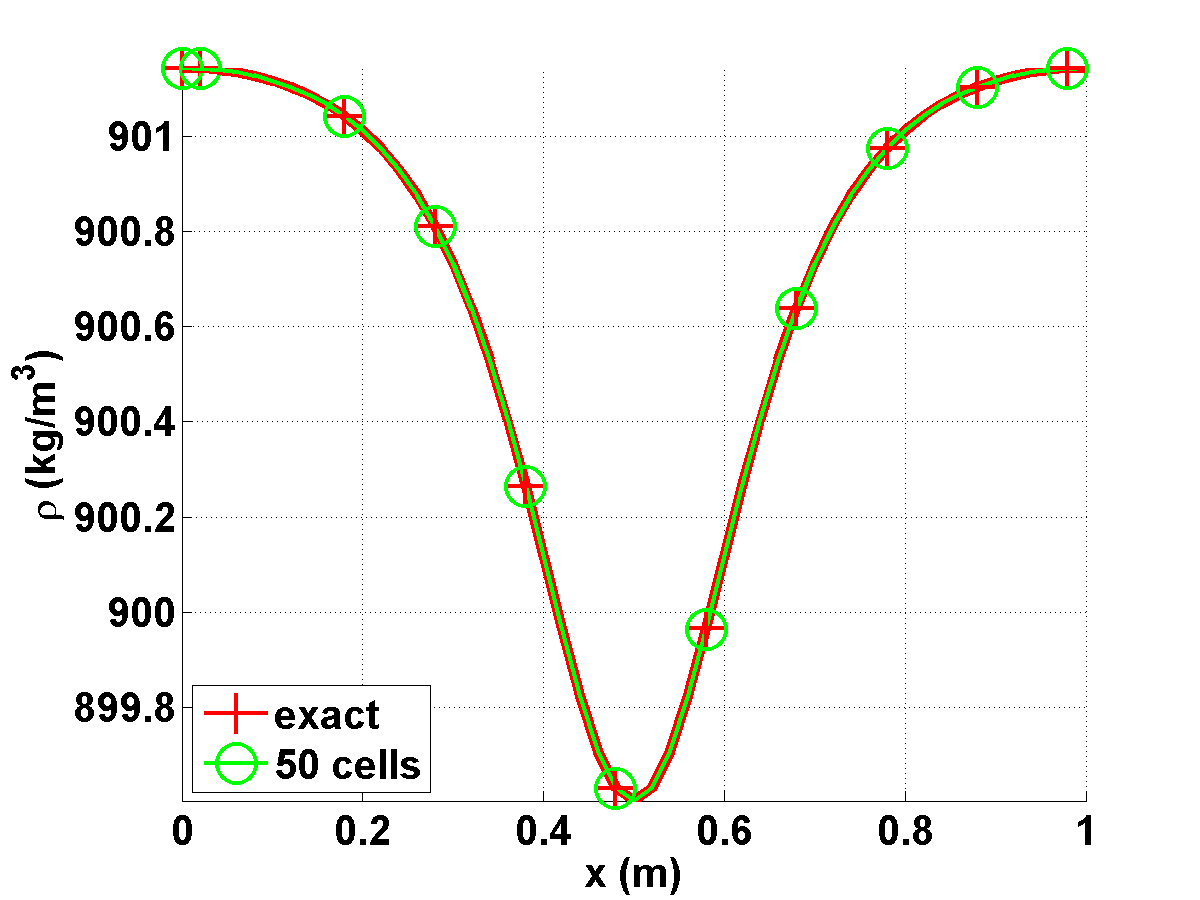
\includegraphics[scale=.50]{figures/liquid_velocity_numerical_and_exact_50.png}
                \caption{Velocity solution at steady-state.}
                \label{fig:1d_nozzle_liq_vel}
        \end{subfigure}%
        %add desired spacing between images, e. g. ~, \quad, \qquad etc. 
          %(or a blank line to force the subfigure onto a new line)
        \begin{subfigure}[b]{0.495\textwidth}
                \centering
                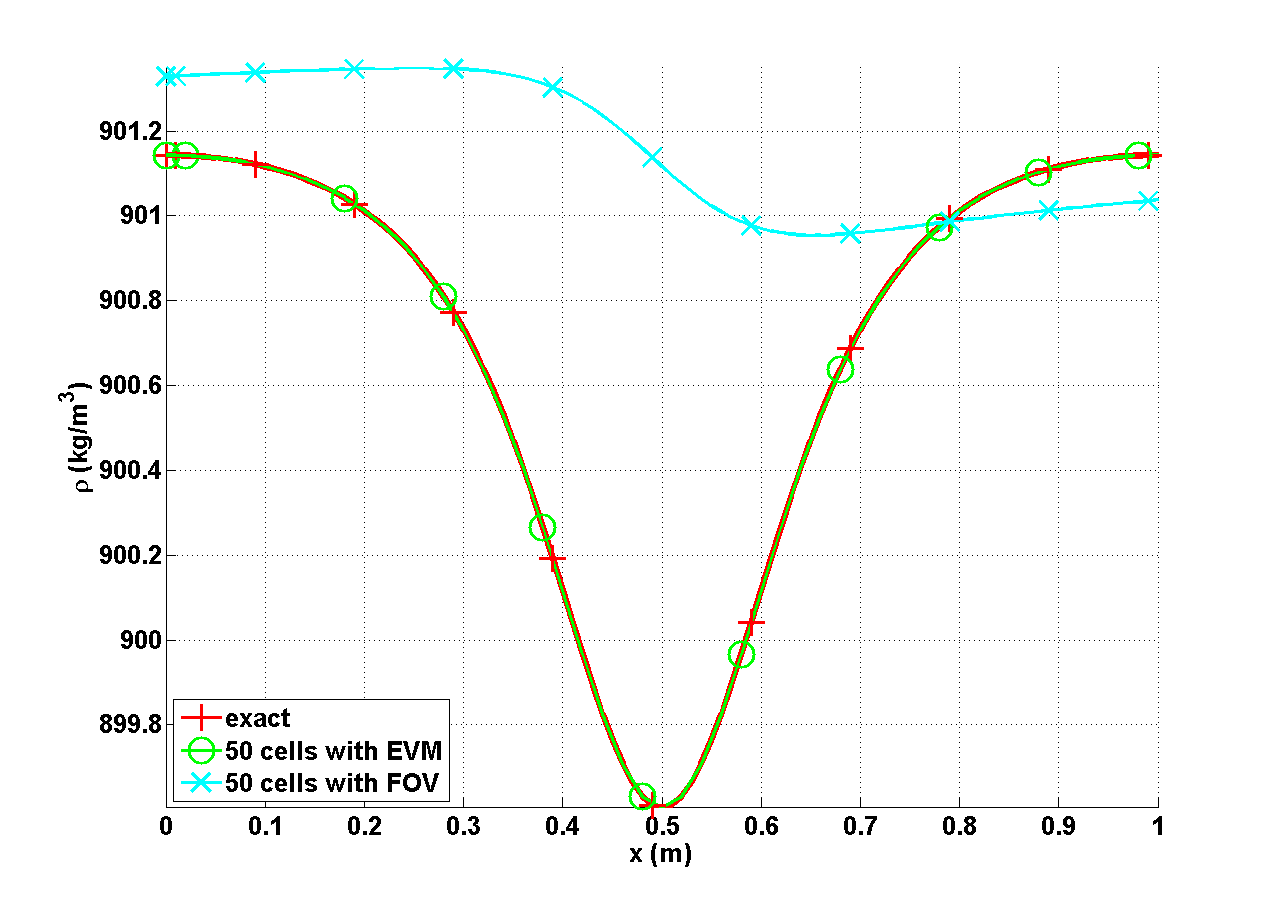
\includegraphics[scale=.50]{figures/liquid_density_numerical_and_exact_50.png}
                \caption{Density solution at steady-state}
                \label{fig:1d_nozzle_liq_density}
        \end{subfigure}
         %add desired spacing between images, e. g. ~, \quad, \qquad etc. 
          %(or a blank line to force the subfigure onto a new line)
        \begin{subfigure}[b]{0.495\textwidth}
                \centering
                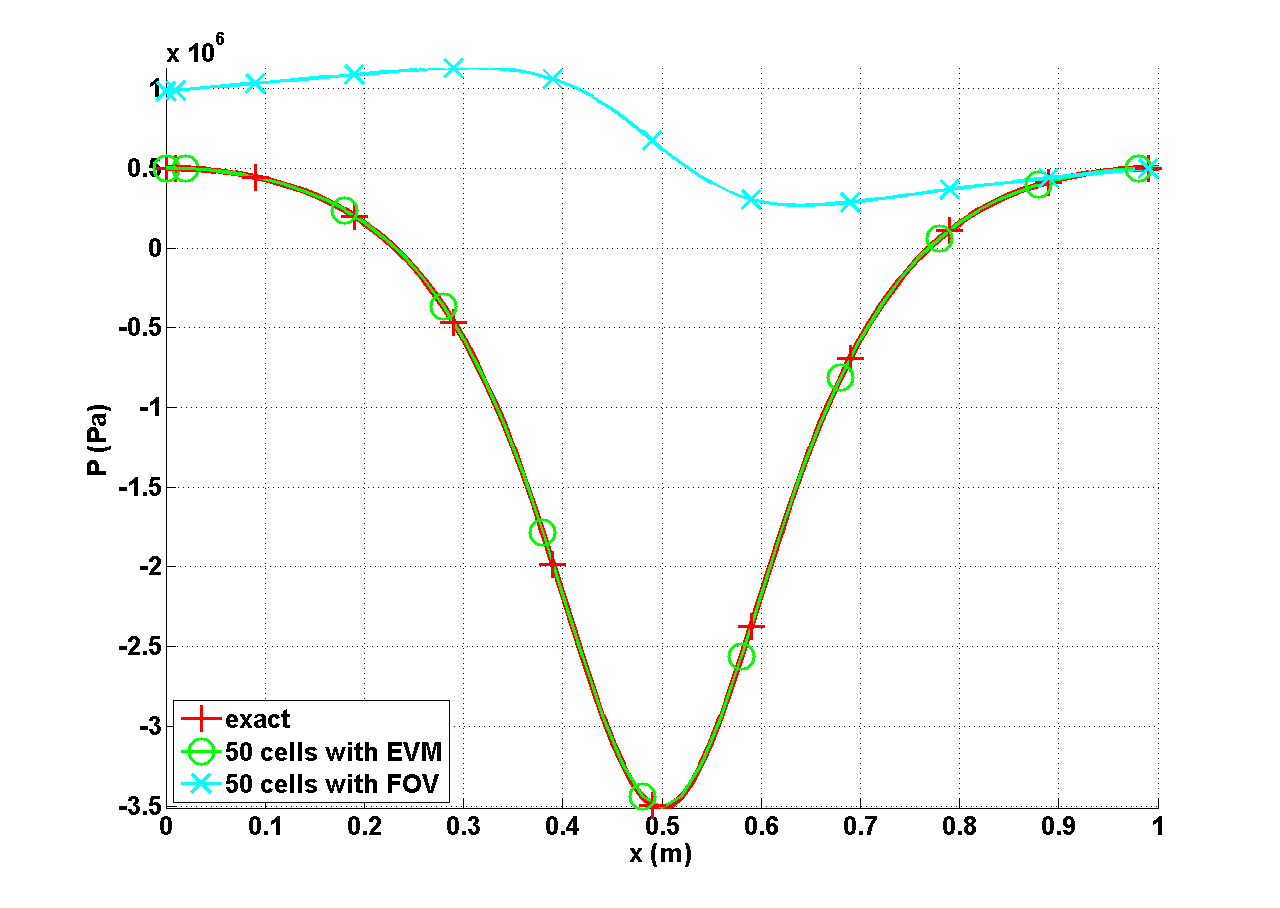
\includegraphics[scale=.50]{figures/liquid_pressure_numerical_and_exact_50.png}
                \caption{Pressure solution at steady-state.}
                \label{fig:1d_nozzle_liq_press}
        \end{subfigure}
          %add desired spacing between images, e. g. ~, \quad, \qquad etc. 
          %(or a blank line to force the subfigure onto a new line)
        \begin{subfigure}[b]{0.495\textwidth}
                \centering
                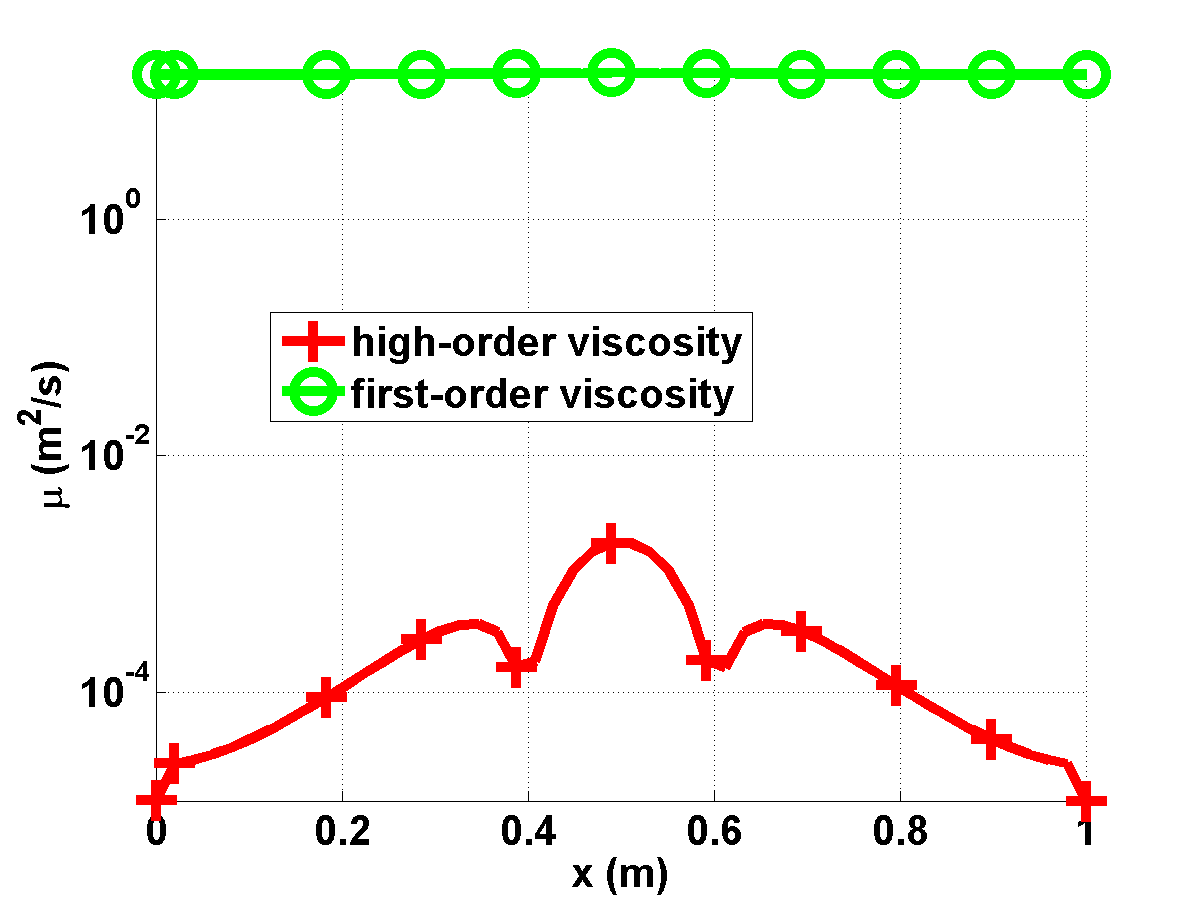
\includegraphics[scale=.50]{figures/liquid_viscosity_numerical50.png}
                \caption{Viscosity coefficients at steady-state.}
                \label{fig:1d_nozzle_liq_visc}
        \end{subfigure}
        \caption{Steady-state solution for liquid phase in a $1$-D convergent-divergent nozzle with an uniform mesh of $50$ cells.}\label{fig:1d_liq_nozzle}
\end{figure}
The numerical and exact solutions of the velocity, pressure and density given in \fig{fig:1d_liq_nozzle} for a fairly coarse mesh ($50$ cells) perfectly overlap: it is noted that the numerical solution is symmetric with respect to the nozzle throat located in $x=0.5m$. The second-order viscosity coefficient  is very small compare to the first-order one as expected: (i) the numerical solution is smooth as shown in \fig{fig:1d_nozzle_liq_visc} and (ii) the flow is in a low Mach regime and thus isentropic . A convergence study was performed using the exact solution as a reference: the L$1$ and L$2$ norms of the error and the corresponding convergence rates are computed at steady-state on various uniform mesh from $4$ to $256$ cells. The results for linear polynomials $\mathbb{Q}_1$ are reported in \tbl{tbl:l1_norm_liq} and \tbl{tbl:l2_norm_liq} for the primitive variables: density, velocity and pressure.
\begin{table}[H]
\begin{center}
 \caption{\label{tbl:l1_norm_liq} L$1$ norm of the error for the liquid phase in a $1$-D convergent-divergent nozzle at steady-state.}
 \begin{tabular}{|c|c|c|c|c|c|c|c|c|}
 \hline
   cells & density & rate & pressure & rate & velocity & rate \\
 \hline
$4$ &   $2.8037$ $10^{-1}$ & $-$ & $8.4705e$ $10^{5}$ & $-$ & $7.2737$                   & $-$\\
  \hline
$8$  &  $1.3343$ $10^{-1}$ & $1.0713$ & $4.7893e$ $10^{5}$ & $0.24227$ & $6.1493$                   & $0.074683$\\
   \hline
$16$ & $2.9373$ $10^{-2}$ & $2.1835$ & $1.0613e$ $10^{5}$ & $2.3247$ & $1.2275$& $2.4501$\\
 \hline
$32$ & $5.1120$ $10^{-3}$ & $2.5225$ & $1.8446$ $10^{4}$ & $2.6959$ & $1.8943$ $10^{-1}$ & $3.0966$\\
 \hline
$64$ & $1.0558$ $10^{-3}$ & $2.2755$ & $3.7938$ $10^{3}$ & $2.3207$ & $3.7919$ $10^{-2}$ & $2.3323$\\
 \hline
$128$&$2.3712$ $10^{-4}$ & $2.1547$ & $8.4471$ $10^{2}$ & $2.0624$ & $8.5517$ $10^{-3}$ & $2.0473$\\
 \hline
$256$&$5.6058$ $10^{-5}$& $2.0806$ & $1.9839$ $10^{2}$ & $2.0478$ & $2.0475$ $10^{-3}$ & $1.9833$\\
 \hline
 $512$&$1.3278$ $10^{-5}$& $2.0778$ & $46.622$ & $2.0478$ & $4.9516$ $10^{-4}$ & $1.9669$\\
 \hline
\end{tabular}
\end{center}
\nonumber
\end{table}
\begin{table}[H]
\begin{center}
 \caption{\label{tbl:l2_norm_liq} L$2$ norm of the error for the liquid phase in a $1$-D convergent-divergent nozzle at steady-state.}
 \begin{tabular}{|c|c|c|c|c|c|c|c|c|}
 \hline
   cells & density & rate & pressure & rate & velocity & rate \\
 \hline
$4$ &   $3.106397$ $10^{-1}$ & $-$ & $5.254445$ $10^{5}$ & $-$ & $3.288543$                   & $-$\\
  \hline
$8$  &  $7.491623$ $10^{-2}$ & $2.07$ & $1.636966$ $10^{5}$ & $1.60$ & $1.823880$                   & $0.90$\\
   \hline
$16$ & $2.079858$ $10^{-2}$ & $1.80$ & $4.627338$ $10^{4}$ & $1.75$ & $4.990605$ $10^{-1}$ & $1.83$\\
 \hline
$32$ & $5.329627$ $10^{-3}$ & $1.90$ & $1.180287$ $10^{4}$ & $1.92$ & $1.261018$ $10^{-1}$ & $1.93$\\
 \hline
$64$ & $1.341583$ $10^{-3}$ & $1.94$ & $2.967104$ $10^{3}$ & $1.98$ & $3.160914$ $10^{-2}$ & $1.99$\\
 \hline
$128$&$3.359766$ $10^{-4}$ & $1.99$ & $7.428087$ $10^{2}$ & $1.99$ & $7.907499$ $10^{-3}$ & $1.99$\\
 \hline
$256$&$8.403859$ $10^{-5}$& $1.99$ & $1.857861$ $10^{2}$ & $1.99$ & $1.977292$ $10^{-3}$ & $1.99$\\
 \hline
 $512$&$2.10075$ $10^{-5}$& $1.99$ & $27.048$ & $1.99$ & $4.9516$ $10^{-4}$ & $1.99$\\
 \hline
\end{tabular}
\end{center}
\nonumber
\end{table}
It is observed that the convergence rate for the L$1$ and L$2$ norm of the error is $2$: the entropy viscosity method conserves the high-order accuracy when the numerical solution is smooth, and the new definition of the entropy viscosity coefficient seems to behave as expected in the low Mach limit.
%---------------------------------------------------------------------------------------------------
\subsection{Steam in a $1$-D divergent-convergent nozzle} \label{sec:steam_nozzle}
%---------------------------------------------------------------------------------------------------
Instead of liquid water, we now simulate a flow of steam using the exact same $1$-D geometry, initial conditions and boundary conditions as in \sect{sec:liquid_nozzle}. The Stiffened gas equation of state is still used but with different parameters that are given in \tbl{tbl:stff_gas_eos_vap}: steam is a gas and compressible effects will become dominant. 
\begin{table}[H]
\begin{center}
 \caption{\label{tbl:stff_gas_eos_vap} Stiffened Gas Equation of State parameters for steam.}
 \begin{tabular}{|c|c|c|c|}
 \hline
$\gamma$ & $C_v$ $(J\cdot kg^{-1} \cdot K^{-1})$ & $P_{\infty}$ $(Pa)$ & $q$ $(J \cdot kg^{-1})$ \\
 \hline
1.43 & 1040 & 0 & $2030.10^3$   \\
 \hline
\end{tabular}
\end{center}
\end{table}
The pressure difference applied between the inlet and outlet is large enough to make the steam accelerates through the nozzle and result in the formation of shock in the divergent part. The behavior is different from what is observed for the liquid water phase in \sect{sec:liquid_nozzle} because of the liquid to gas density ratio that is of $1000$. Even though a shock forms, an exact solution at steady-state is still available \cite{nozzle_exact}. The objective of this section is to show that using the new definition of the viscosity coefficient in \eqt{eq:final_def_visc_coeff}, the shock can be correctly resolved without spurious oscillation. The steady-state numerical solution is shown in \fig{fig:1d_vap_nozzle} and was run with a mesh of $1600$ cells.
\begin{figure}[H]
        \centering
        \begin{subfigure}[b]{0.495\textwidth}
                \centering
                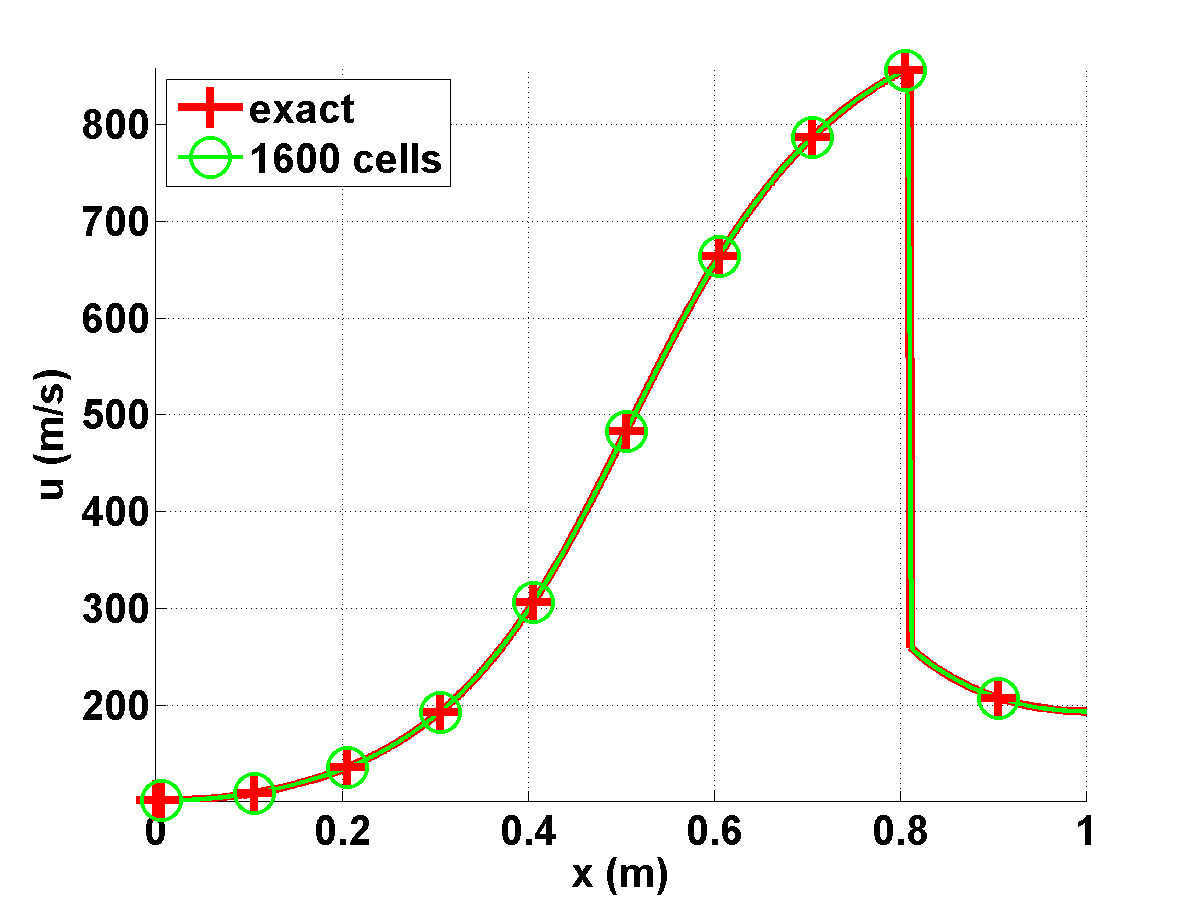
\includegraphics[scale=.50]{figures/vapor_velocity_numerical_and_exact_1600.png}
                \caption{Velocity solution at steady-state.}
                \label{fig:1d_nozzle_vap_vel}
        \end{subfigure}%
        %add desired spacing between images, e. g. ~, \quad, \qquad etc. 
          %(or a blank line to force the subfigure onto a new line)
        \begin{subfigure}[b]{0.495\textwidth}
                \centering
                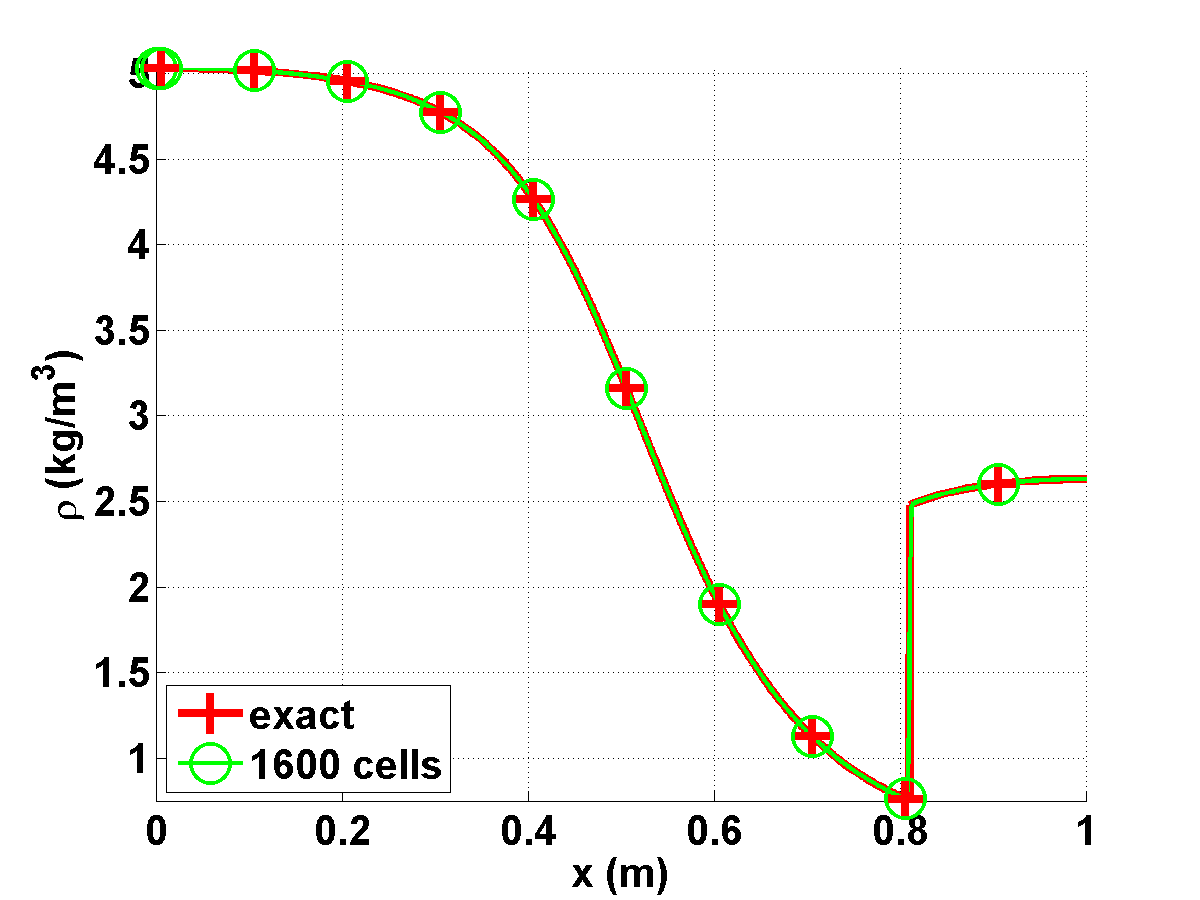
\includegraphics[scale=.50]{figures/vapor_density_numerical_and_exact_1600.png}
                \caption{Density solution at steady-state}
                \label{fig:1d_nozzle_vap_density}
        \end{subfigure}
         %add desired spacing between images, e. g. ~, \quad, \qquad etc. 
          %(or a blank line to force the subfigure onto a new line)
        \begin{subfigure}[b]{0.495\textwidth}
                \centering
                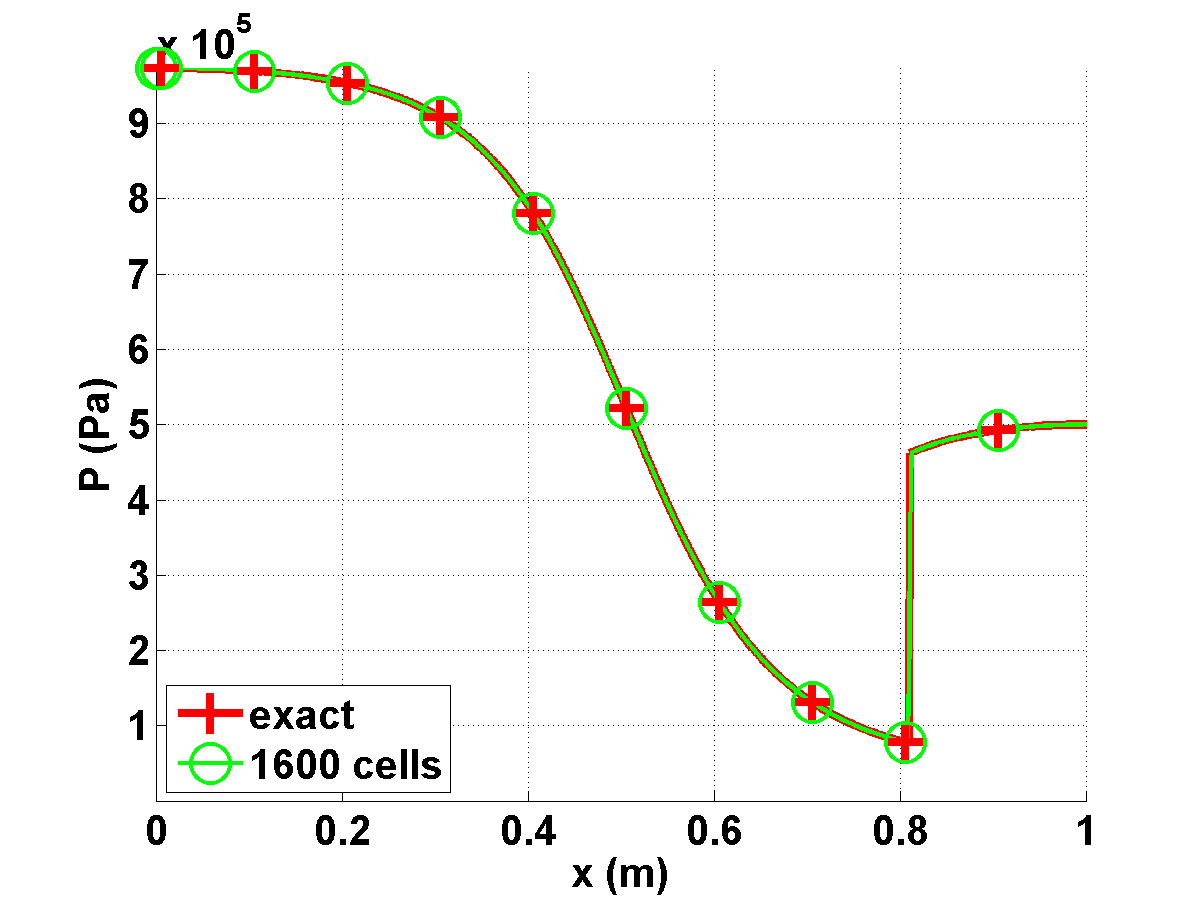
\includegraphics[scale=.50]{figures/vapor_pressure_numerical_and_exact_1600.png}
                \caption{Pressure solution at steady-state.}
                \label{fig:1d_nozzle_vap_press}
        \end{subfigure}
          %add desired spacing between images, e. g. ~, \quad, \qquad etc. 
          %(or a blank line to force the subfigure onto a new line)
        \begin{subfigure}[b]{0.495\textwidth}
                \centering
                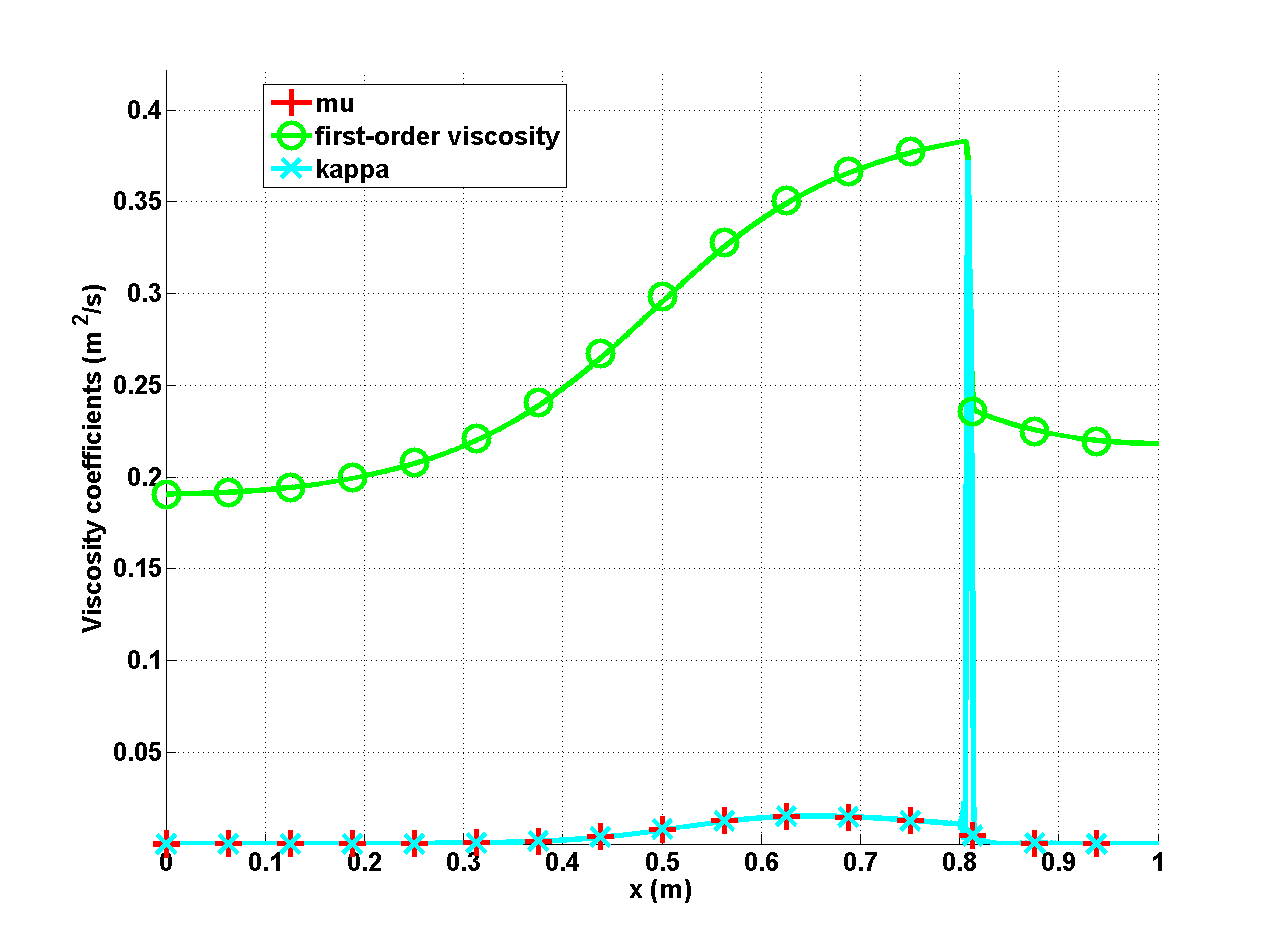
\includegraphics[scale=.50]{figures/vapor_viscosity_numerical1600.png}
                \caption{Viscosity coefficients at steady-state.}
                \label{fig:1d_nozzle_vap_visc}
        \end{subfigure}
        \caption{Steady-state solution for vapor phase in a $1$-D convergent-divergent nozzle.}\label{fig:1d_vap_nozzle}
\end{figure}
The steady-state solution of the density, velocity and pressure are given in \fig{fig:1d_nozzle_vap_vel}, \fig{fig:1d_nozzle_vap_density} and \fig{fig:1d_nozzle_vap_press}. The steady-solution displays a shock around $x=0.8m$ and match the exact solution. In \fig{fig:1d_nozzle_vap_visc}, the first- and second-order viscosity coefficients are log plotted at steady-state: the second-order viscosity coefficient is peaked in the shock region around $x=0.8m$ as expected, and saturate to the first-order viscosity coefficient. The profile also displays another peak at $x=0.5m$ that corresponds to the position of the sonic point for a $1$-D convergent-divergent nozzle: this particular point is known to develop small instabilities that are detected when computing the jumps of the pressure and density gradients. Anywhere else, the second-order viscosity coefficient is small. In order to prove convergence of the numerical solution to the exact solution, a convergence study is performed. Because of the presence of a shock, second-order accuracy cannot be achieved. However, the convergence rate of a numerical solution containing a shock  is known and expected to be of $1$ and $1/2$ when computing the L$1$ and L$2$ norms of the error, respectively (see Theorem 9.3 in \cite{convergence_book}). Results are reported in \tbl{tbl:l1_norm_vap} and \tbl{tbl:l2_norm_vap} for the primitive variables: density, velocity and pressure.
\begin{table}[H]
\begin{center}
 \caption{\label{tbl:l1_norm_vap} L$1$ norm of the error for the vapor phase in a $1$-D convergent-divergent nozzle at steady-state.}
 \begin{tabular}{|c|c|c|c|c|c|c|c|c|}
 \hline
   cells & density & rate & pressure & rate & velocity & rate \\
 \hline
$5$ &   $0.72562$ $10^{-1}$ & $-$ & $1.5657$ $10^{5}$ & $-$ & $173.69$                   & $-$\\
  \hline
$10$  &  $0.4165$ $10^{-1}$ & $0.80088$ & $9.6741$ $10^{4}$ & $0.63425$ & $120.69$ & $0.52519$\\
   \hline
$20$ & $0.20675$ $10^{-1}$ & $1.0104$ & $4.9193$ $10^{4}$ & $0.96971$ & $72.149$& $0.74228$\\
 \hline
$40$ & $0.093703$ $10^{-1}$ & $1.1417$ & $2.0103$ $10^{4}$ & $0.72728$ & $34.716$& $1.0554$\\
 \hline
$80$ & $0.047328$ $10^{-1}$ & $0.9854$ & $1.0208$ $10^{4}$ & $0.9777$ & $16.082$& $1.1101$\\
 \hline
$160$&$0.023965$ $10^{-2}$ & $0.9817$ & $5.1969$ $10^{3}$ & $0.9739$ & $7.9573$& $1.0150$\\
 \hline
$320$&$0.020768$ $10^{-2}$& $0.9886$ & $2.5116$ $10^{3}$ & $1.0490$ & $3.7812$& $1.0734$\\
 \hline
 $640$&$0.0059715$ $10^{-2}$& $1.0160$ & $1.2754$ $10^{3}$ & $0.9776$ & $1.8353$& $1.0428$\\
 \hline
\end{tabular}
\end{center}
\nonumber
\end{table}
\begin{table}[H]
\begin{center}
 \caption{\label{tbl:l2_norm_vap} L$2$ norm of the error for the vapor phase in a $1$-D convergent-divergent nozzle at steady-state.}
 \begin{tabular}{|c|c|c|c|c|c|c|c|c|}
 \hline
   cells & density & rate & pressure & rate & velocity & rate \\
 \hline
$5$ &   $9.7144$ $10^{-1}$ & $-$ & $2.0215$ $10^{5}$ & $-$ & $236.94$                   & $-$\\
  \hline
$10$  &  $5.9718$ $10^{-1}$ & $0.70195$ & $1.3024$ $10^{5}$ & $0.63425$ & $166.56$ & $0.50854$\\
   \hline
$20$ & $2.9503$ $10^{-1}$ & $1.0173$ & $6.6503$ $10^{4}$ & $0.96971$ & $103.36$& $0.68831$\\
 \hline
$40$ & $1.8193$ $10^{-1}$ & $0.69747$ & $4.0171$ $10^{4}$ & $0.72728$ & $66.374$& $0.6390$\\
 \hline
$80$ & $1.3366$ $10^{-1}$ & $0.44485$ & $2.3163$ $10^{4}$ & $0.43576$ & $42.981$& $0.62692$\\
 \hline
$160$&$9.6638$ $10^{-2}$ & $0.46790$ & $1.7263$ $10^{4}$ & $0.42413$ & $31.717$& $0.43844$\\
 \hline
$320$&$7.0896$ $10^{-2}$& $0.44688$ & $1.2763$ $10^{4}$ & $0.43571$ & $23.138$& $0.45499$\\
 \hline
 $640$&$5.2191$ $10^{-2}$& $0.44190$ & $9.4217$ $10^{3}$ & $0.43790$ & $16.910$& $0.45238$\\
 \hline
\end{tabular}
\end{center}
\nonumber
\end{table}
The convergence rates for the L$1$ and L$2$ norms of the error are close to the theoretical values which prove convergence of the numerical solution to the exact solution.\\
It is also interesting to investigate the effect of the first-order viscosity onto the steady-state solution. In \fig{fig:1d_nozzle_vap_fo_ev}, the steady-state velocity profile is plotted when using the first- and second-order viscosity coefficients: the main difference between the two numerical solution is in the resolution of the shock around $x=0.8m$. The first-order viscosity coefficient is by definition more dissipative and will smooth out the solution. In the other hand, the high-order viscosity better resolves the shock and allow high-order accuracy away from the shock region. It is also noted that the numerical solution obtained with the first-order viscosity coefficient is satisfying: this is due to the nature of the solution that contains a standing shock, and thus, will force the shock to form even with large artificial dissipation. 
\begin{figure}[H]
\centering
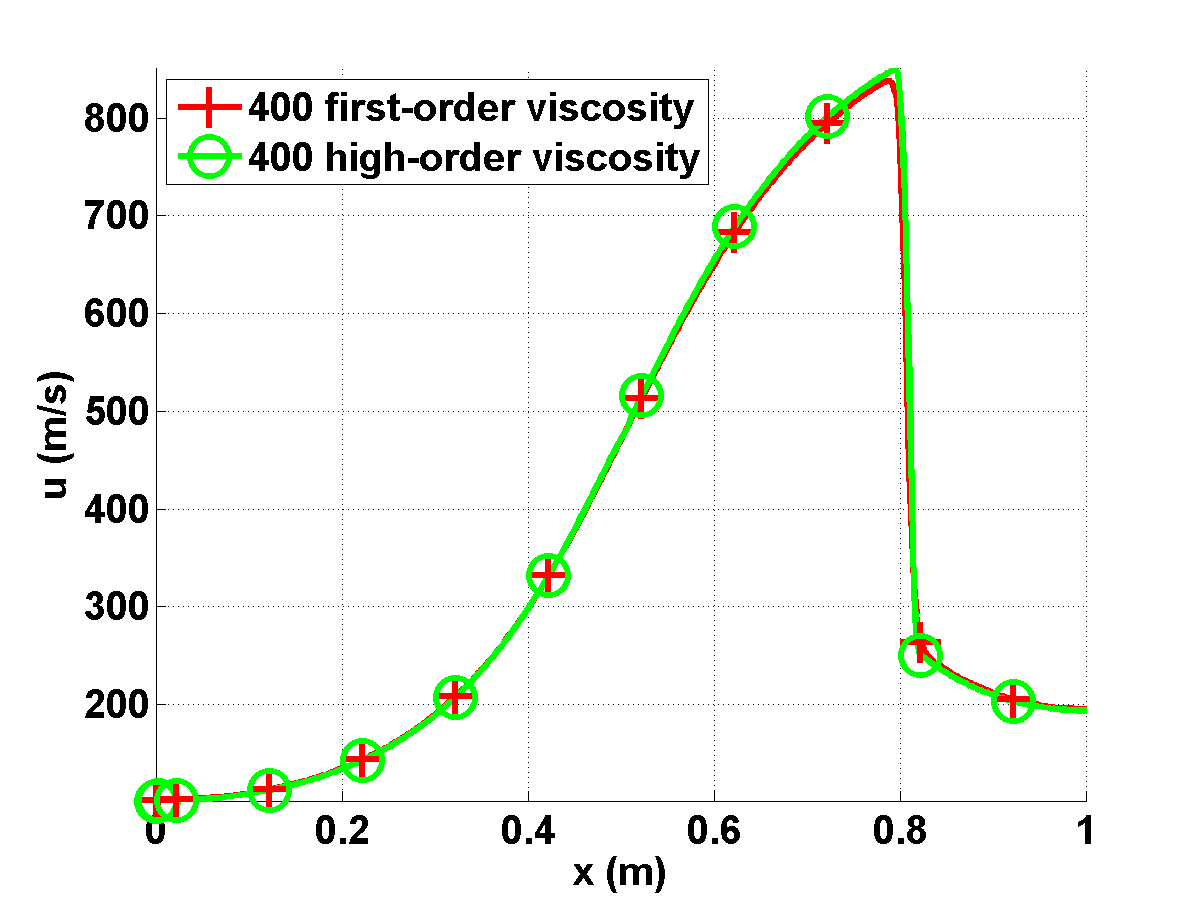
\includegraphics[scale=.50]{figures/vapor_velocity_fo_and_ev_400.png}
\caption{Velocity profile at steady-state with the first- and second-order viscosity for a mesh with $400$ cells.}
\label{fig:1d_nozzle_vap_fo_ev}
\end{figure}
%---------------------------------------------------------------------------------------------------
\subsection{Leblanc shock tube} \label{sec:Leblanc}
%---------------------------------------------------------------------------------------------------
The $1$-D Leblanc shock tube is a Riemann problem designed to test the robustness and the accuracy of the stabilization method. The initial conditions are given in \tbl{tbl:ic_leblanc}. The ideal gas equation of state is used to compute the fluid pressure with the following heat capacity ratio $\gamma=5/3$.
\begin{table}[H]
\begin{center}
 \caption{\label{tbl:ic_leblanc} Initial conditions for the $1$-D Leblanc shock tube.}
 \begin{tabular}{|c|c|c|c|}
 \hline
   & $\rho$ & $u$ & $e$ \\
 \hline
left & $1.$ & $0.$ & $0.1$ \\
  \hline
  right & $10^{-3}$ & $0.$ & $10^{-7}$ \\
  \hline
\end{tabular}
\end{center}
\nonumber
\end{table}
This test is computationally challenging because of the large left to right pressure ratio.
The computational domain consists of a $1$-D pipe of length $L=9m$ with an interface located at $x=2m$. At $t=0.s$, the interface is removed, allowing the fluid to move. The numerical solution is run until $t=4.s$ and the density, momentum and total energy profiles are given in \fig{fig:1d_leblanc_vel}, \fig{fig:1d_leblanc_density} and \fig{fig:1d_leblanc_press}, respectively, along with the exact solution. The viscosity coefficients are also plotted in \fig{fig:1d_leblanc_visc}. These plots were  run with three different uniform mesh of $800$, $3200$ and $6000$ cells and a constant time step $\Delta t = 10^{-3}s.$.
\begin{figure}[H]
        \centering
        \begin{subfigure}[b]{0.495\textwidth}
                \centering
                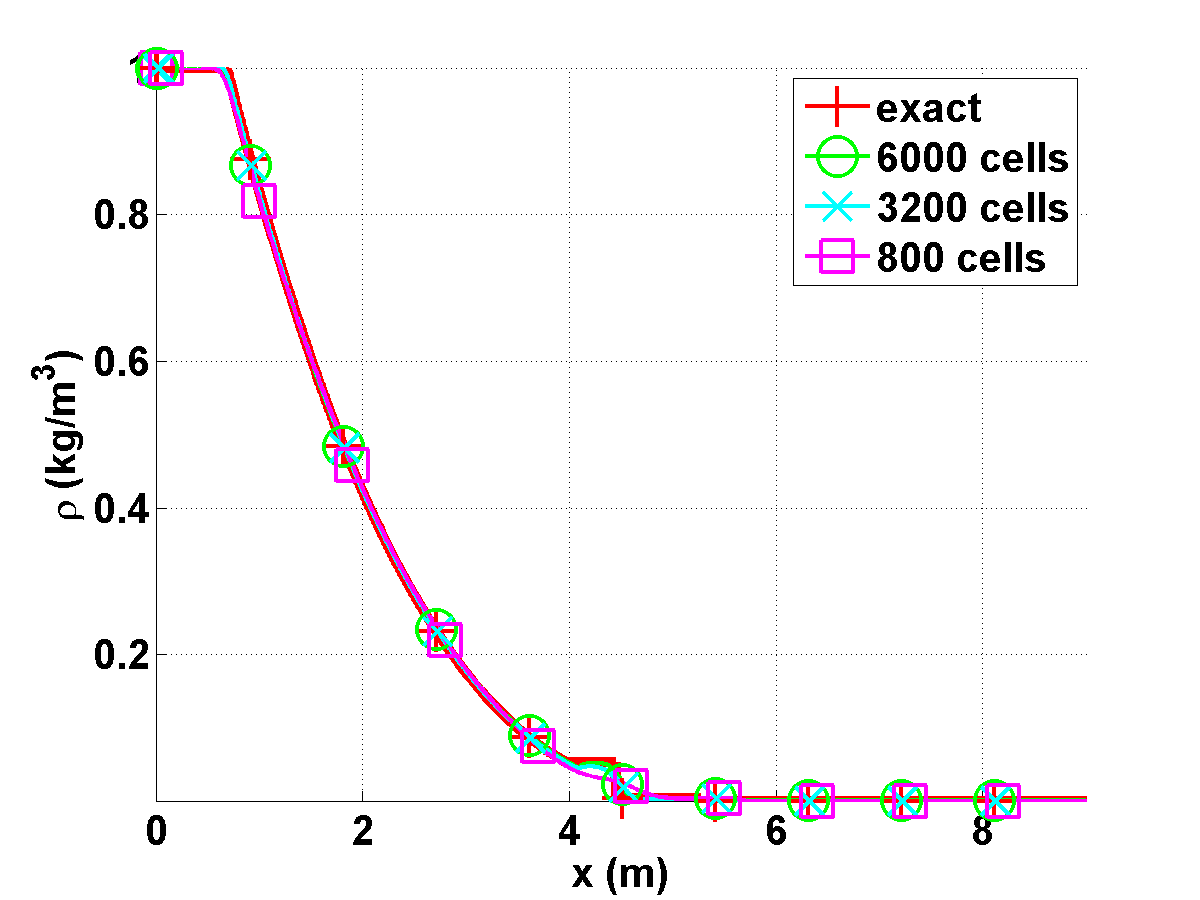
\includegraphics[scale=.50]{figures/Leblanc_exact_and_numerical_stt_density_6000.png}
                \caption{Density profile.}
                \label{fig:1d_leblanc_vel}
        \end{subfigure}%
        %add desired spacing between images, e. g. ~, \quad, \qquad etc. 
          %(or a blank line to force the subfigure onto a new line)
        \begin{subfigure}[b]{0.495\textwidth}
                \centering
                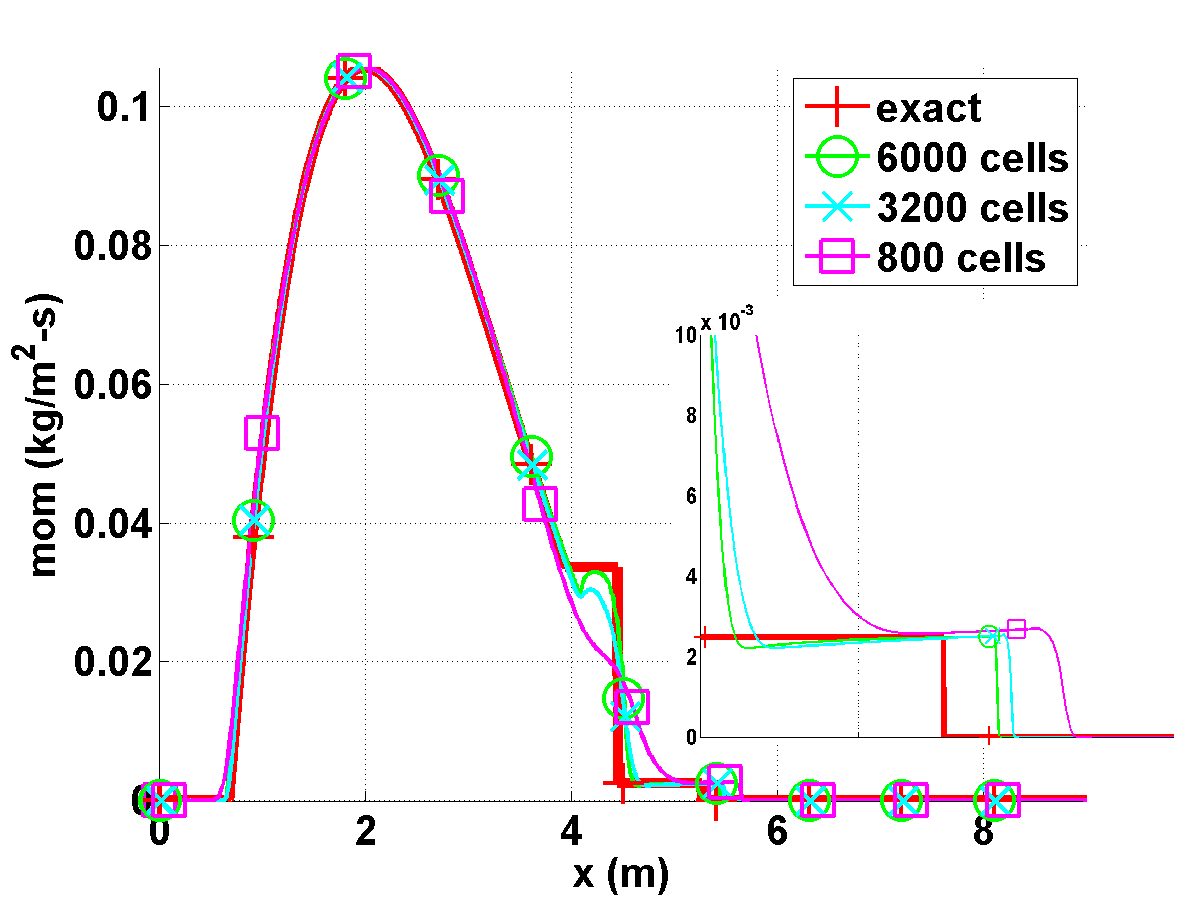
\includegraphics[scale=.50]{figures/Leblanc_exact_and_numerical_stt_momentum_6000.png}
                \caption{Velocity profile.}
                \label{fig:1d_leblanc_density}
        \end{subfigure}
         %add desired spacing between images, e. g. ~, \quad, \qquad etc. 
          %(or a blank line to force the subfigure onto a new line)
        \begin{subfigure}[b]{0.495\textwidth}
                \centering
                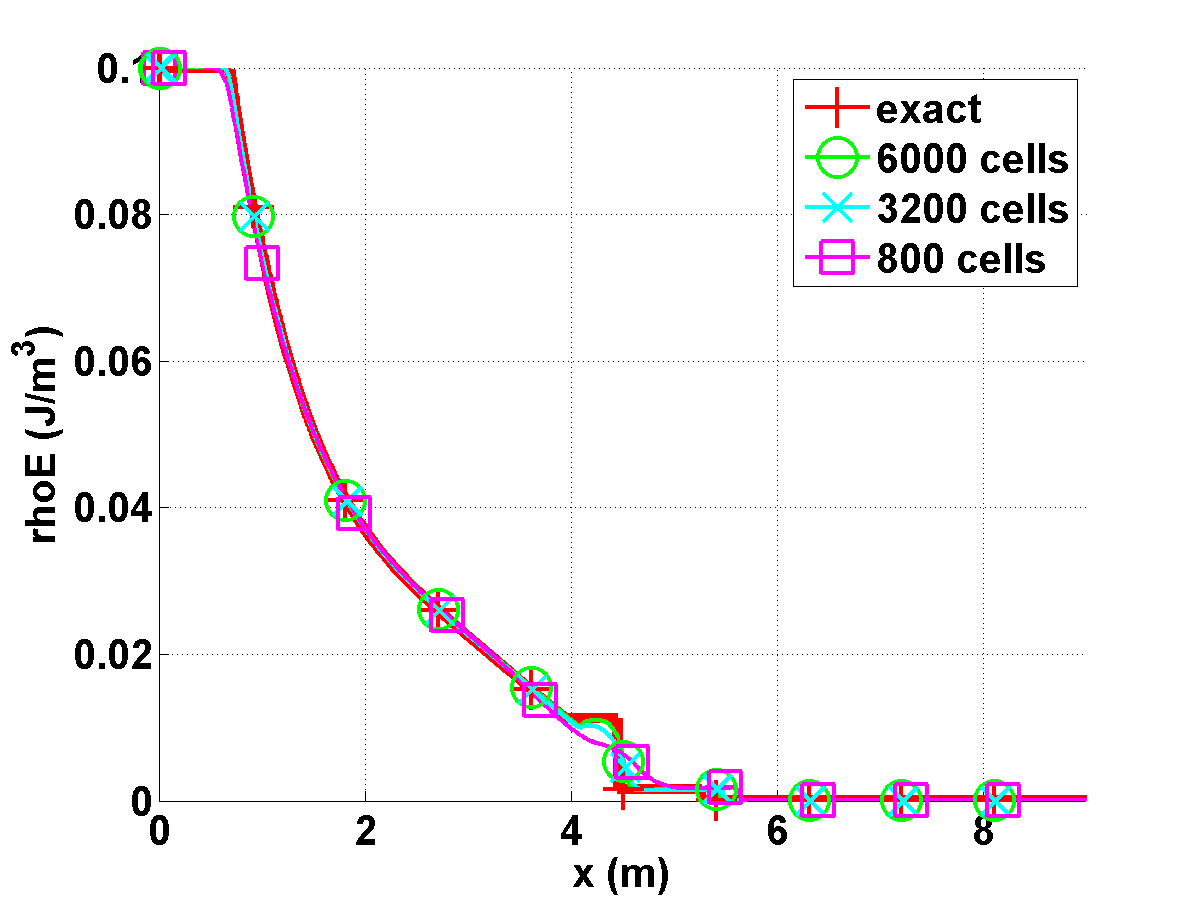
\includegraphics[scale=.50]{figures/Leblanc_exact_and_numerical_stt_total_energy_6000.png}
                \caption{Pressure profile.}
                \label{fig:1d_leblanc_press}
        \end{subfigure}
          %add desired spacing between images, e. g. ~, \quad, \qquad etc. 
          %(or a blank line to force the subfigure onto a new line)
        \begin{subfigure}[b]{0.495\textwidth}
                \centering
                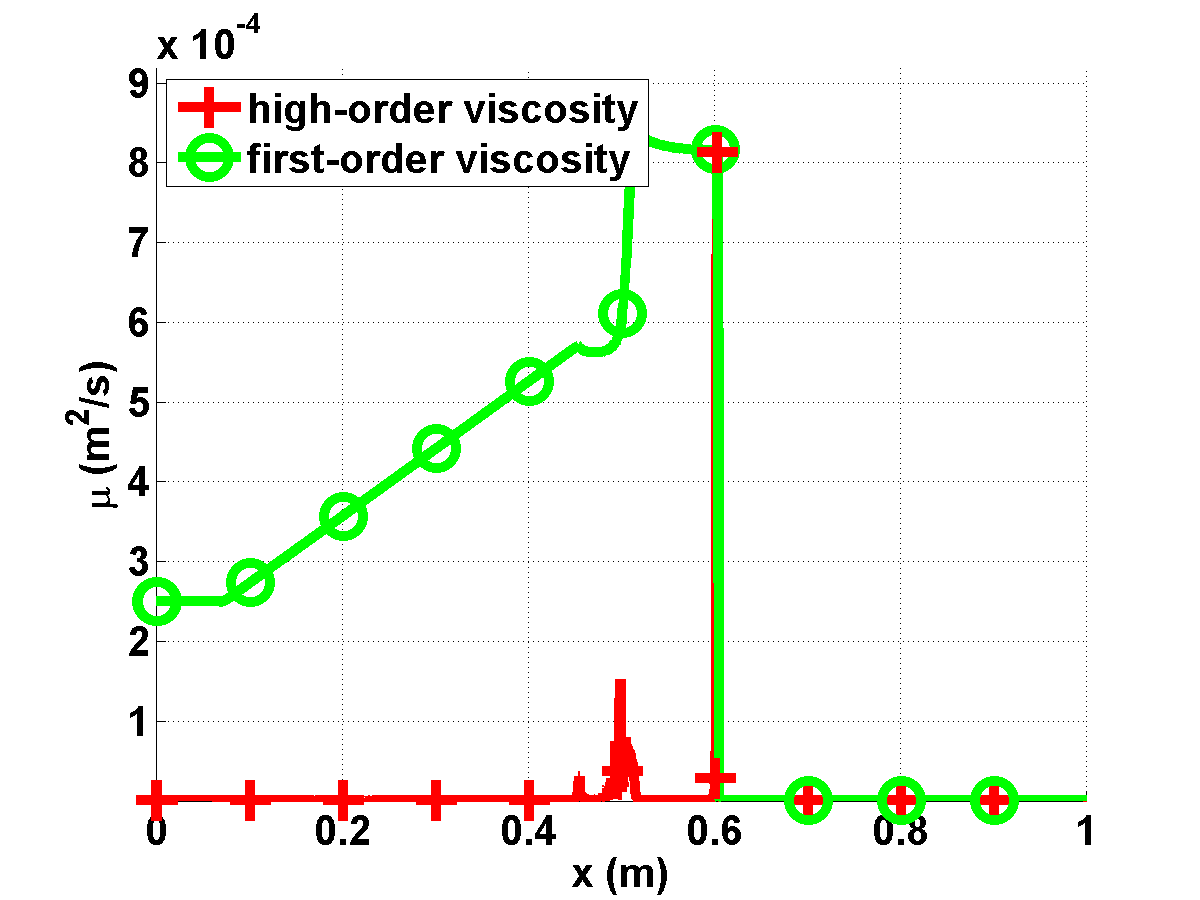
\includegraphics[scale=.50]{figures/Leblanc_viscosity_numerical_6000.png}
                \caption{Viscosity coefficients.}
                \label{fig:1d_leblanc_visc}
        \end{subfigure}
        \caption{Numerical solution for the $1$-D Leblanc shock tube at $t=4.s$.}\label{fig:1d_lebalnc}
\end{figure}
 The density, momentum and total energy profiles given in \fig{fig:1d_lebalnc} do not display any oscillations. In \fig{fig:1d_leblanc_density}, the shock region is zoomed in for better resolution: the shock is well resolved and do not show any oscillation. It is also observed that the shock position of the numerical solution converges to the exact position when refining the mesh. The contact wave is shown in \fig{fig:1d_leblanc_density} at $x=4.5m$. The second-order viscosity coefficient profile is shown in \fig{fig:1d_leblanc_visc} and behaves as expected: it saturates to the first-order viscosity in the shock region and thus prevent oscillations from forming. In the contact wave at $x=4.5m$, a smaller peak is observed that is due to the presence of the jumps in the definition of the second-order viscosity coefficient (\eqt{eq:final_def_visc_coeff}).  \\
Once again, a convergence study is performed in order to prove convergence of the numerical solution to the exact solution. As for the vapor phase in the $1$-D nozzle (\sect{sec:steam_nozzle}), the expected convergence rate for the L$1$ and L$2$ norms of the error are $1$ and $1/2$, respectively. The exact solution was obtained by running a $1$-D Riemann solver and used as a reference solution to compute the L$1$ and L$2$-norms of the error that are reported in \tbl{tbl:l1_norm_leblanc} and \tbl{tbl:l2_norm_leblanc} for the conservative variables: density, momentum and total energy.
\begin{table}[H]
\begin{center}
 \caption{\label{tbl:l1_norm_leblanc} L$1$ norm of the error for the $1$-D Leblanc test at $t=4.s$.}
 \begin{tabular}{|c|c|c|c|c|c|c|}
 \hline
   cells & density & rate & momentum & rate \\
 \hline
$100$ &   $1.0354722$ $10^{-2}$ & $-$ & $3.5471714$ $10^{-3}$ & $-$ \\
  \hline
$200$  &  $7.2680512$ $10^{-3}$ & $0.51064841$ & $2.5933119$ $10^{-3}$ & $0.45187331$ \\
   \hline
$400$ & $5.0825628$ $10^{-3}$   & $0.51601245$ & $2.0668092$ $10^{-3}$ & $0.32739054$ \\
 \hline
$800$ & $3.4025056$ $10^{-3}$   & $0.57895861$ & $1.4793838$ $10^{-3}$ & $0.48240884$ \\
 \hline
$1600$ & $2.1649953$ $10^{-3}$  & $0.65223363$ & $9.7152832$ $10^{-4}$ & $0.6066684$ \\
 \hline
$3200$&$1.2465433$ $10^{-3}$    & $0.79643094$ & $5.5937409$ $10^{-4}$ & $0.79644263$ \\
 \hline
$6400$& $6.4476928$ $10^{-4}$    & $0.95107804$ & $3.0244198$ $10^{-4}$ & $0.88715502$ \\
 \hline
 $12800$&$3.3950948$ $10^{-4}$  & $0.92533116$ & $1.5958118$ $10^{-4}$ & $0.9223679$ \\
 \hline
 \end{tabular}
 \begin{tabular}{|c|c|c|}
\hline
cells & total energy & rate \\ \hline
 $100$ & $0.0014033046$                   & $-$\\ \hline
  $200$  & $9.8611746$ $10^{-4}$& $0.5089968$\\ \hline
  $400$ & $7.7844421$ $10^{-4}$ & $0.34116585$\\ \hline
  $800$ & $5.5702549$ $10^{-4}$ & $0.48285029$\\ \hline
  $1600$ & $3.5720171$ $10^{-4}$ & $0.64100438$\\ \hline
  $3200$ & $2.0491799$ $10^{-4}$ & $0.80169235$\\ \hline
  $6400$ & $1.0914891$ $10^{-4}$ & $0.90874889$\\ \hline
   $12800$&$5.7909794$ $10^{-5}$ & $0.91441847$\\ \hline
\end{tabular}
\end{center}
\nonumber
\end{table}
\begin{table}[H]
\begin{center}
 \caption{\label{tbl:l2_norm_leblanc} L$2$ norm of the error for the $1$-D Leblanc test at $t=4.s$.}
 \begin{tabular}{|c|c|c|c|c|c|c|}
 \hline
   cells & density & rate & momentum & rate \\
 \hline
$100$ &   $5.7187851$ $10^{-3}$ & $-$ & $1.7767236$ $10^{-3}$ & $-$ \\
  \hline
$200$  &  $3.8995238$ $10^{-3}$ & $0.55241073$ & $1.4913161$ $10^{-3}$ & $0.25263314$ \\
   \hline
$400$ & $2.8103526$ $10^{-3}$   & $0.4725468$ & $1.3305301$ $10^{-3}$ & $0.164585$ \\
 \hline
$800$ & $2.1081933$ $10^{-3}$   & $0.41474398$ & $1.1398931$ $10^{-3}$ & $0.22310254$ \\
 \hline
$1600$ & $1.5731052$ $10^{-3}$  & $0.42239201$ & $9.0394227$ $10^{-4}$ & $0.33459602$ \\
 \hline
$3200$&$1.0610667$ $10^{-3}$    & $0.56809979$ & $6.2735595$ $10^{-4}$ & $0.52694639$ \\
 \hline
$6400$&$7.3309974$ $10^{-4}$    & $0.53343397$ & $4.4545754$ $10^{-4}$ & $0.49399631$ \\
 \hline
 $12800$&$5.1020991$ $10^{-4}$  & $0.52291857$ & $3.1266758$ $10^{-4}$ & $0.5106583$ \\
 \hline
\end{tabular}
\begin{tabular}{|c|c|c|}
\hline
cells & total energy & rate \\ \hline
$100$ & $7.6112265$  $10^{-4}$& $-$\\ \hline
$200$ & $5.5497308$ $10^{-4}$& $0.45571115$\\ \hline
$400$ & $4.6063172$ $10^{-4}$ & $0.26880405$\\ \hline
$800$ & $3.7798953$ $10^{-4}$ & $0.28526749$\\ \hline
$1600$ & $2.9584646$ $10^{-4}$ & $0.35349763$\\ \hline
$3200$ & $2.054455$ $10^{-4}$ & $0.52609289$\\ \hline
$6400$ & $1.4670834$ $10^{-4}$ & $0.48580482$\\ \hline
$12800$ & $1.0299897$ $10^{-5}$ & $0.51032105$\\  \hline
\end{tabular}
\end{center}
\nonumber
\end{table}
The convergence rates are close to the expected values which prove convergence of the numerical solution to the exact solution.
%---------------------------------------------------------------------------------------------------
\subsection{Typical $1$-D shock tubes \cite{Toro}} \label{sec:1d_toro}
%---------------------------------------------------------------------------------------------------
%---------------------------------------------------------------------------------------------------
\subsection{Subsonic flow over a $2$-D cylinder} \label{sec:cylinder}
%---------------------------------------------------------------------------------------------------
The flow of a fluid over a $2$-D cylinder is a typical benchmark case to test the behavior of a numerical method in the low Mach regime. For this test, an analytical solution is available in the incompressible limit or low Mach limit (REFS) and often referred to as potential flow. The main features of the potential flow are the following:
\begin{itemize}
\item The solution is symmetric: the iso-mach number lines are used to asses the symmetry of the numerical solution.
\item The velocity at the top of the cylinder is twice the incoming velocity set at the inlet.
\item The pressure fluctuations are proportional to the inlet Mach number square, as follows: 
\begin{equation}
\tilde{P} = \frac{\max(P) - \min(P)}{\max(P)}  \propto M_{\infty}^2\nonumber
\end{equation}
where $\tilde{P}$ and $M_{\infty}$ are the pressure fluctuations and the inlet Mach number, respectively.
\end{itemize}
The computational domain consists of a $1\times 1$ square with a circular hole of radius $0.05$ in its middle. At the inlet, a subsonic stagnation boundary condition is used: the stagnation pressure and temperature are computed using the following relations, valid for the Stiffened and Ideal gas equation of states:
\begin{equation}
\label{eq:stagnation_relations}
\left\{
\begin{array}{l}
P_0 = P\left( 1 + \frac{\gamma-1}{2} M^2 \right)^{\frac{\gamma-1}{\gamma}} \\
T_0 = T\left( 1 + \frac{\gamma-1}{2} M^2 \right)
\end{array}
\right.
\end{equation}
The static pressure $P_s = 101325$ $Pa$ is set at the subsonic outlet and a static pressure boundary type is used. The implementation of the pressure boundary conditions is done on the model of \cite{SEM}. A solid wall boundary condition is set for the top and bottom walls of the computational domain: the normal velocity is zero since no mass can penetrate the solid body. The mesh is made of triangular cells.\\
The steady-state for Mach numbers ranging from $M_{\infty} = 10^{-3}$ to $M_{\infty} = 10^{-7}$ is shown in \fig{fig:cylinder}. The iso-Mach lines are drawn with $50$ intervals ranging from $10^{-8}$ to $2M_{\infty}$, and allow to assess the symmetry of the numerical solution.
%\begin{figure}[H]
%        \centering
        \begin{figure}[H]%{0.495\textwidth}
                \centering
                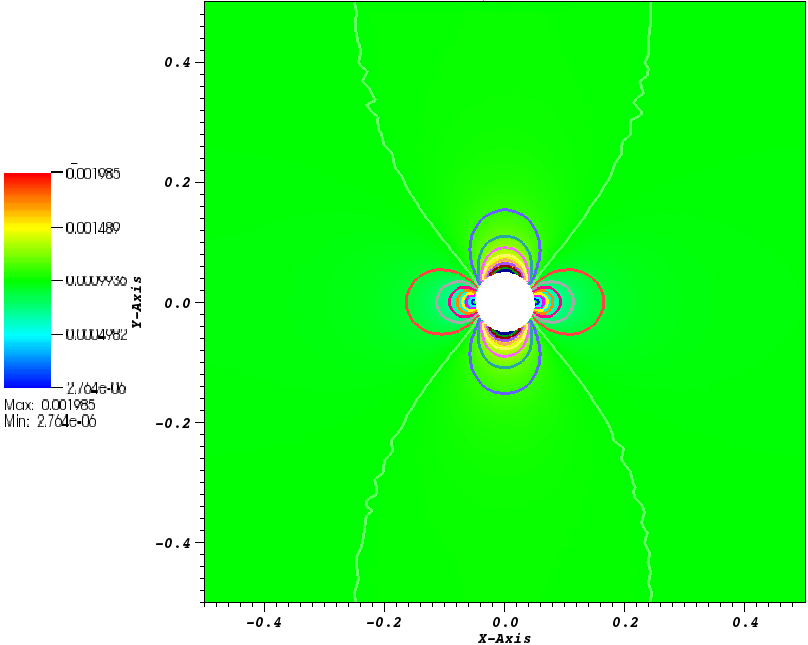
\includegraphics[scale=.50]{figures/CylinderMach1em3.png}
                \caption{Steady-state solution at $M_{\infty}=10^{-3}$.}
                \label{fig:cyl_1em3}
        \end{figure}%
        %add desired spacing between images, e. g. ~, \quad, \qquad etc. 
          %(or a blank line to force the subfigure onto a new line)
          
        \begin{figure}[H]%{0.495\textwidth}
                \centering
                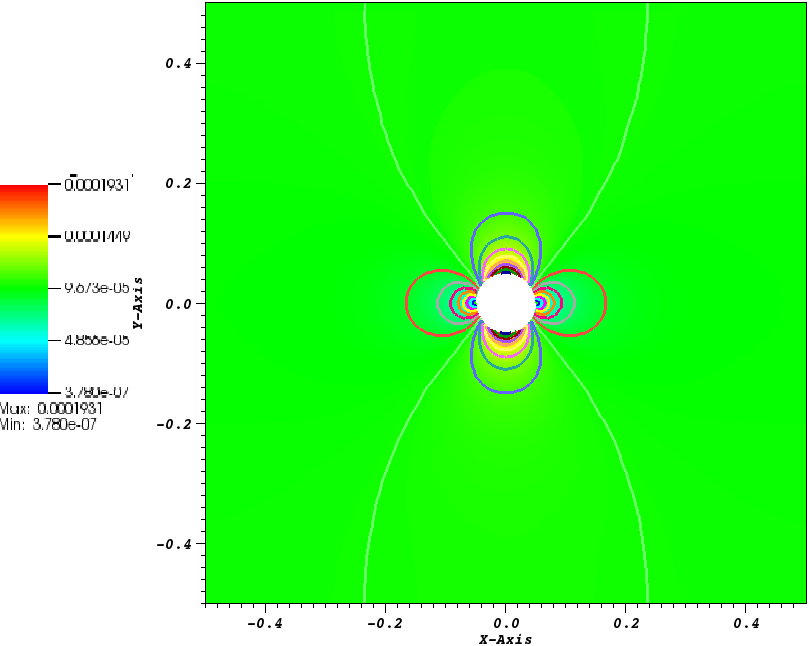
\includegraphics[scale=.50]{figures/CylinderMach1em4.png}
                \caption{Steady-state solution at $M_{\infty}=10^{-4}$.}
                \label{fig:cyl_1em4}
        \end{figure}   
         %add desired spacing between images, e. g. ~, \quad, \qquad etc. 
          %(or a blank line to force the subfigure onto a new line)
          
        \begin{figure}[H]%{0.495\textwidth}
                \centering
                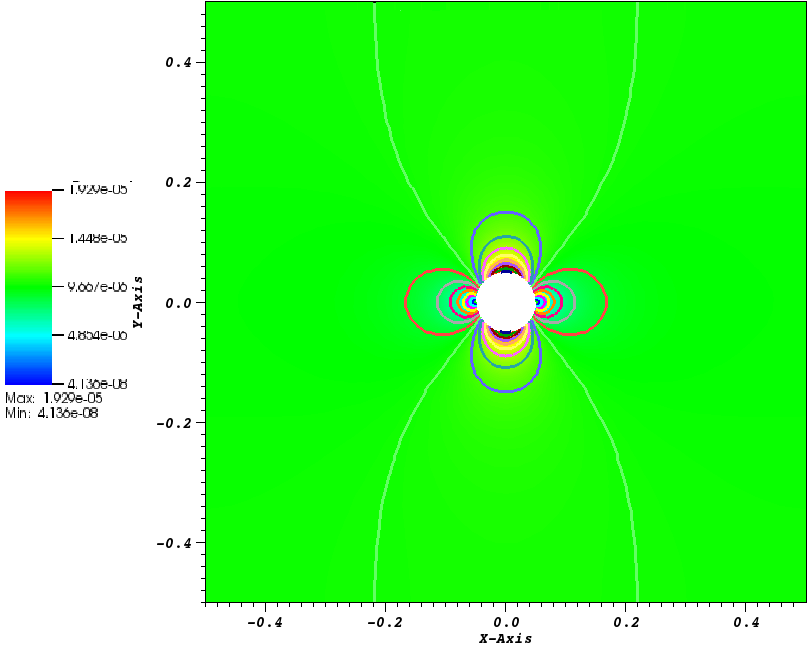
\includegraphics[scale=.50]{figures/CylinderMach1em5.png}
                \caption{Steady-state solution at $M_{\infty}=10^{-5}$.}
                \label{fig:cyl_1em5}
        \end{figure}
          %add desired spacing between images, e. g. ~, \quad, \qquad etc. 
          %(or a blank line to force the subfigure onto a new line)
          
        \begin{figure}[H]%{0.495\textwidth}
                \centering
                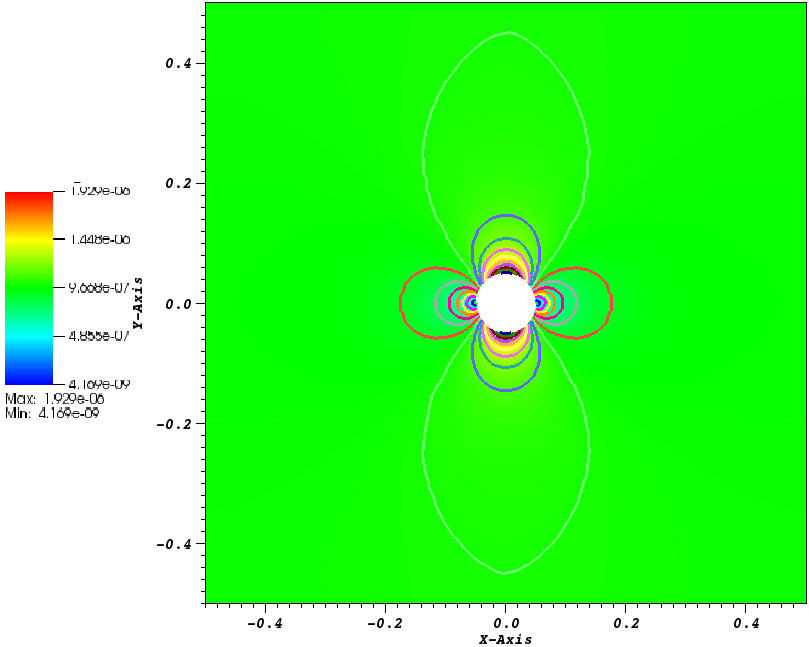
\includegraphics[scale=.50]{figures/CylinderMach1em7.png}
                \caption{Steady-state solution at $M_{\infty}=10^{-7}$.}
                \label{fig:cyl_1em7}
        \end{figure}
%        \caption{Steady-state solution for a subsonic flow over a $2$-D cylinder.}\label{fig:cylinder}
%\end{figure}
In \tbl{tbl:velocity_ratio}, the velocity at the top of the cylinder and at the inlet are given for the different values of the Mach number presented in \fig{fig:cylinder}. The ratio of the inlet velocity to the velocity at the top of cylinder is also computed and is very close to $2$ as expected.
\begin{table}[H]
\begin{center}
 \caption{\label{tbl:velocity_ratio}Velocity ratio for different Mach numbers.}
\begin{tabular}{|c|c|c|c|}
\hline
Mach number & inlet velocity & velocity at the top of the cylinder & ratio \\ \hline
$10^{-3}$ & $2.348$ $10^{-3}$ & $1.176$ $10^{-3}$& $1.99$ \\ \hline
$10^{-4}$ & $2.285$ $10^{-4}$ & $1.145$ $10^{-4}$& $1.99$ \\ \hline
$10^{-5}$ & $2.283$ $10^{-5}$ & $1.144$ $10^{-5}$ & $1.99$ \\ \hline
$10^{-6}$ & $2.283$ $10^{-6}$ & $1.144$ $10^{-6}$ & $1.99$ \\ \hline
$10^{-7}$ & $2.283$ $10^{-7}$ & $1.144$ $10^{-7}$ & $1.99$ \\ \hline
\end{tabular}
\end{center}
\nonumber
\end{table}
%---------------------------------------------------------------------------------------------------
\subsection{Subsonic flow over a $2$-D hump} \label{sec:hump}
%---------------------------------------------------------------------------------------------------
This is a another example of an internal flow configuration. It consist of a channel of height $L=1$ $m$ and length $3L$, with a circular bump of length $L$ and thickness $0.1L$. The bump is located on the bottom wall at a distance $L$ from the inlet. The system is initialized with an uniform pressure $P=101325$ $Pa$ and temperature $T=300$ $K$. The initial velocity is computed from the Mach number, $M_{\infty}$, the pressure, the temperature and the Ideal Gas equation of state with the heat capacity $C_v = 717$ $J/kg-K$ and the heat capacity ratio $\gamma=1.4$. At the inlet, a subsonic stagnation boundary condition is used and the stagnation pressure and temperature are computed using \eqt{eq:stagnation_relations}.
The static pressure $P_s = 101325$ $Pa$ is set at the subsonic outlet. An uniform grid is used to get the numerical solution until steady-state is reached. The results are shown in \fig{fig:2d_hump_mach_0p7}, \fig{fig:2d_hump_mach_0p01}, \fig{fig:2d_hump_mach_0p0001} and \fig{fig:2d_hump_mach_0p0000001} for the inlet Mach numbers $M_{\infty}=0.7$, $M_{\infty}=0.01$, $M_{\infty}=10^{-4}$ and $M_{\infty}=10^{-7}$, respectively. It is expected that, within the low Mach number range, the solution does not depend on the Mach number and is identical to the solution obtained with an incompressible flow code. On the other hand, for a flow at $M=0.7$, the compressible effects become more important and shock can form.
%\begin{figure}[H]
 %       \centering
        \begin{figure}[H]%{0.5\textwidth}
                \centering
                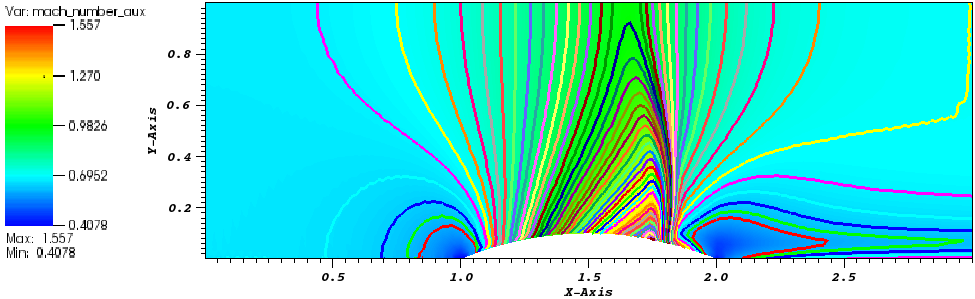
\includegraphics[scale=.50]{figures/Hump2D_mach_0p7.png}
                \caption{Mach $0.7$: iso-Mach lines at steady-state.}
                \label{fig:2d_hump_mach_0p7}
        \end{figure}%
          %add desired spacing between images, e. g. ~, \quad, \qquad etc. 
          %(or a blank line to force the subfigure onto a new line)
        \begin{figure}[H]%{0.5\textwidth}
                \centering
                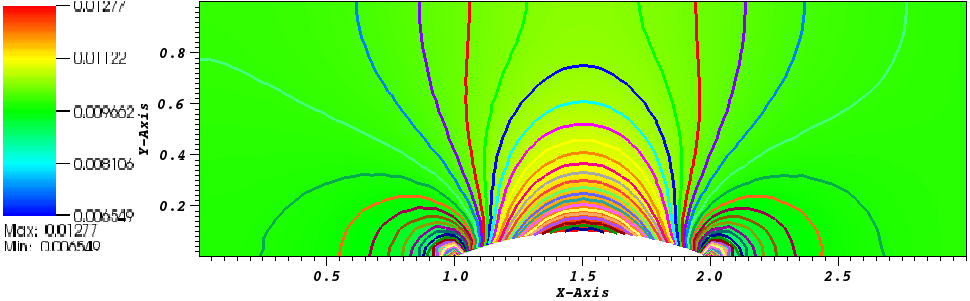
\includegraphics[scale=.50]{figures/Hump2D_mach_0p01.png}
                \caption{Mach $10^{-2}$: iso-Mach lines at steady-state.}
                \label{fig:2d_hump_mach_0p01}
        \end{figure}%
        
        %add desired spacing between images, e. g. ~, \quad, \qquad etc. 
          %(or a blank line to force the subfigure onto a new line)
        \begin{figure}[H]%{0.495\textwidth}
                \centering
                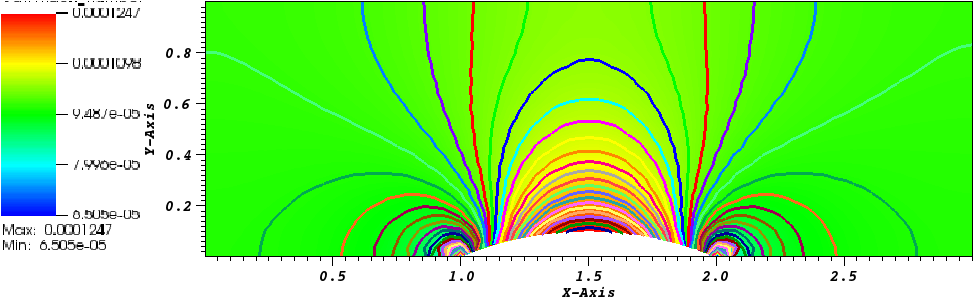
\includegraphics[scale=.50]{figures/Hump2D_mach_1em4.png}
                \caption{Mach $10^{-5}$: iso-Mach lines at steady-state.}
                \label{fig:2d_hump_mach_0p0001}
        \end{figure}
         %add desired spacing between images, e. g. ~, \quad, \qquad etc. 
          %(or a blank line to force the subfigure onto a new line)
        \begin{figure}[H]%{0.495\textwidth}
                \centering
                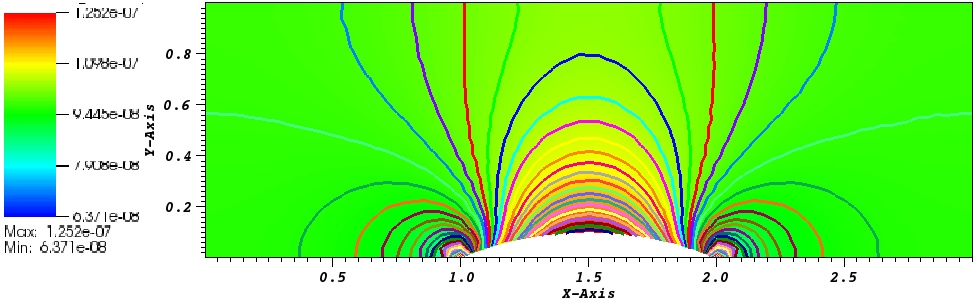
\includegraphics[scale=.50]{figures/Hump2D_mach_1em7.png}
                \caption{Mach $10^{-7}$: iso-Mach lines at steady-state.}
                \label{fig:2d_hump_mach_0p0000001}
        \end{figure}
%        \caption{Steady-state solution for a $2$-D flow over a circular bump.}\label{fig:2d_hump}
%\end{figure}
The results showed in \fig{fig:2d_hump_mach_0p01}, \fig{fig:2d_hump_mach_0p0001} and \fig{fig:2d_hump_mach_0p0000001} correspond to the low Mach regime. The iso-Mach lines are drawn ranging from the minimum and the maximum of each legend with 50 intervals. The steady-state solution is symmetric and does not depend on the value of the inlet Mach number as expected. \\
In \fig{fig:2d_hump_mach_0p7}, the steady-state numerical solution develops a shock: the compressibility effect are no longer negligible. The iso-Mach lines are also plotted with $50$ intervals and ranging from $0.4$ to $1.6$. The shock is well resolved and does not display any instability or spurious oscillation. \\
The results presented in \fig{fig:2d_hump} were obtained with the new definition of the viscosity coefficient (see \eqt{eq:final_def_visc_coeff}), and, illustrate the capabilities of the entropy-viscosity method to adapt to the type of flow (subsonic and transonic flows) without using any tuning parameters, but by just evaluating the entropy residual that is an indicator of the entropy production.    
%---------------------------------------------------------------------------------------------------
\subsection{Supersonic flow in a compression corner} \label{sec:corner}
%---------------------------------------------------------------------------------------------------
This is an example of a supersonic flow over a wedge of angle $15^{\circ}$ where an oblique shock is generated at steady-state. The Mach number upstream of the shock is fixed to $M=2.5$. The initial conditions are uniform: the pressure and temperature are set to $P=101325$ $Pa$ and $T=300$ $K$, respectively. The initial velocity is computed from the upstream Mach number and using the Ideal Gas equation of state with the same parameters as in \sect{sec:hump}. The code is run until steady-state. An analytical solution for this supersonic flow is available and give the downstream to upstream pressure, entropy and Mach number ratios \cite{CompressionCorner}. The analytical and numerical ratios are given in see in \tbl{tbl:corner_exact_sol}, and are very close. 
\begin{table}[H]
\begin{center}
 \caption{\label{tbl:corner_exact_sol} Analytical solution for the supersonic flow on an edge eat $15^{\circ}$ at $M=2.5$.}
 \begin{tabular}{|c|c|c|}
 \hline
   & analytical & numerical \\
    & downstream to upstream ratio & downstream to upstream ratio \\
 \hline
Pressure & 2.47 & 2.467\\
  \hline
Mach number  &  0.74 & 0.741\\
   \hline
  Entropy & 1.03 & 1.026\\ \hline 
\end{tabular}
\end{center}
\nonumber
\end{table}
The inlet is supersonic and therefore, the pressure, temperature and velocity are specified using Dirichlet boundary conditions. The outlet is also supersonic and none of the characteristics enter the domain through this boundary: the values will be computed by the implicit solver.
%\begin{figure}[H]
 %       \centering
        \begin{figure}[H]%{0.52\textwidth}
                \centering
                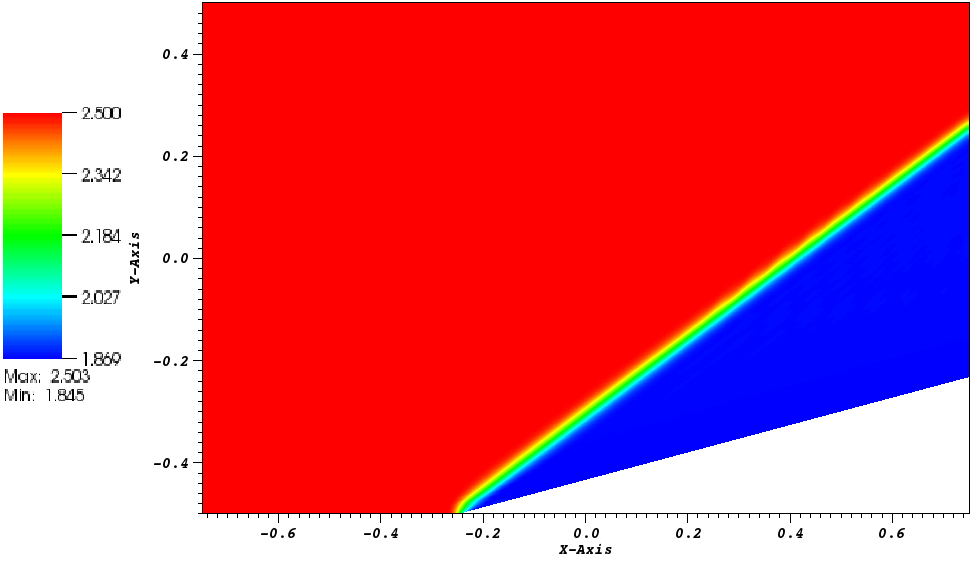
\includegraphics[scale=.50]{figures/CompressionCorner2D_mach.png}
                \caption{Mach solution at steady-state.}
                \label{fig:2d_corner_mach}
        \end{figure}%
          %add desired spacing between images, e. g. ~, \quad, \qquad etc. 
          %(or a blank line to force the subfigure onto a new line)
        \begin{figure}[H]%{0.52\textwidth}
                \centering
                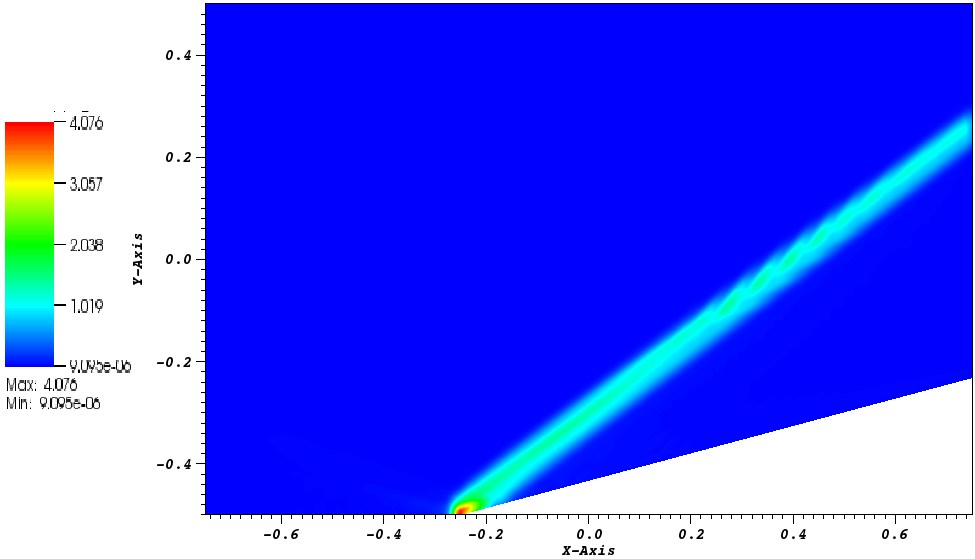
\includegraphics[scale=.50]{figures/CompressionCorner2D_viscosity.png}
                \caption{Viscosity coefficient at steady-state.}
                \label{fig:2d_corner_visc}
        \end{figure}
        
        %add desired spacing between images, e. g. ~, \quad, \qquad etc. 
          %(or a blank line to force the subfigure onto a new line)
        \begin{figure}[H]%{0.49\textwidth}
                \centering
                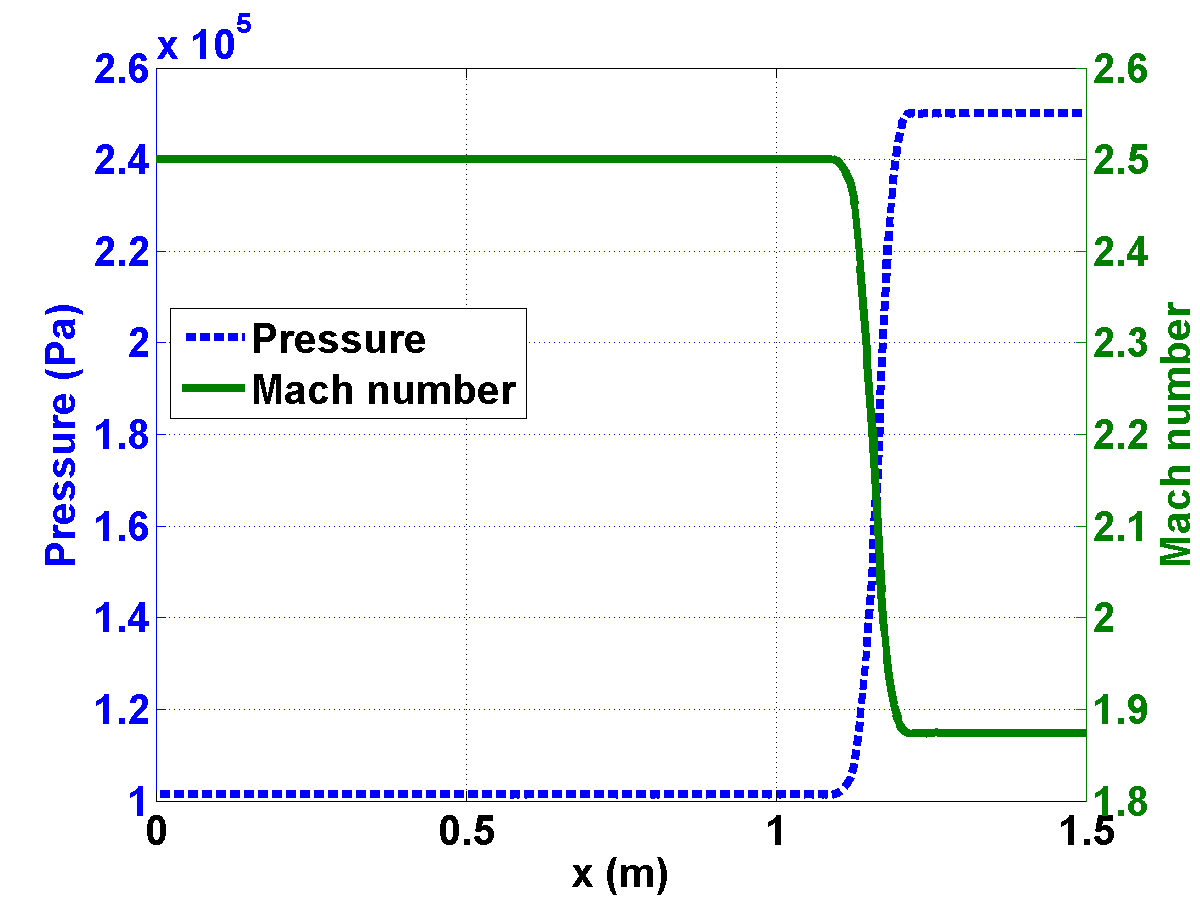
\includegraphics[scale=.50]{figures/mach_number_pressure.png}
                \caption{Pressure and Mach number profiles at steady-state}
                \label{fig:2d_corner_isomach}
        \end{figure}        
          %add desired spacing between images, e. g. ~, \quad, \qquad etc. 
          %(or a blank line to force the subfigure onto a new line)
        \begin{figure}[H]%{0.49\textwidth}
                \centering
                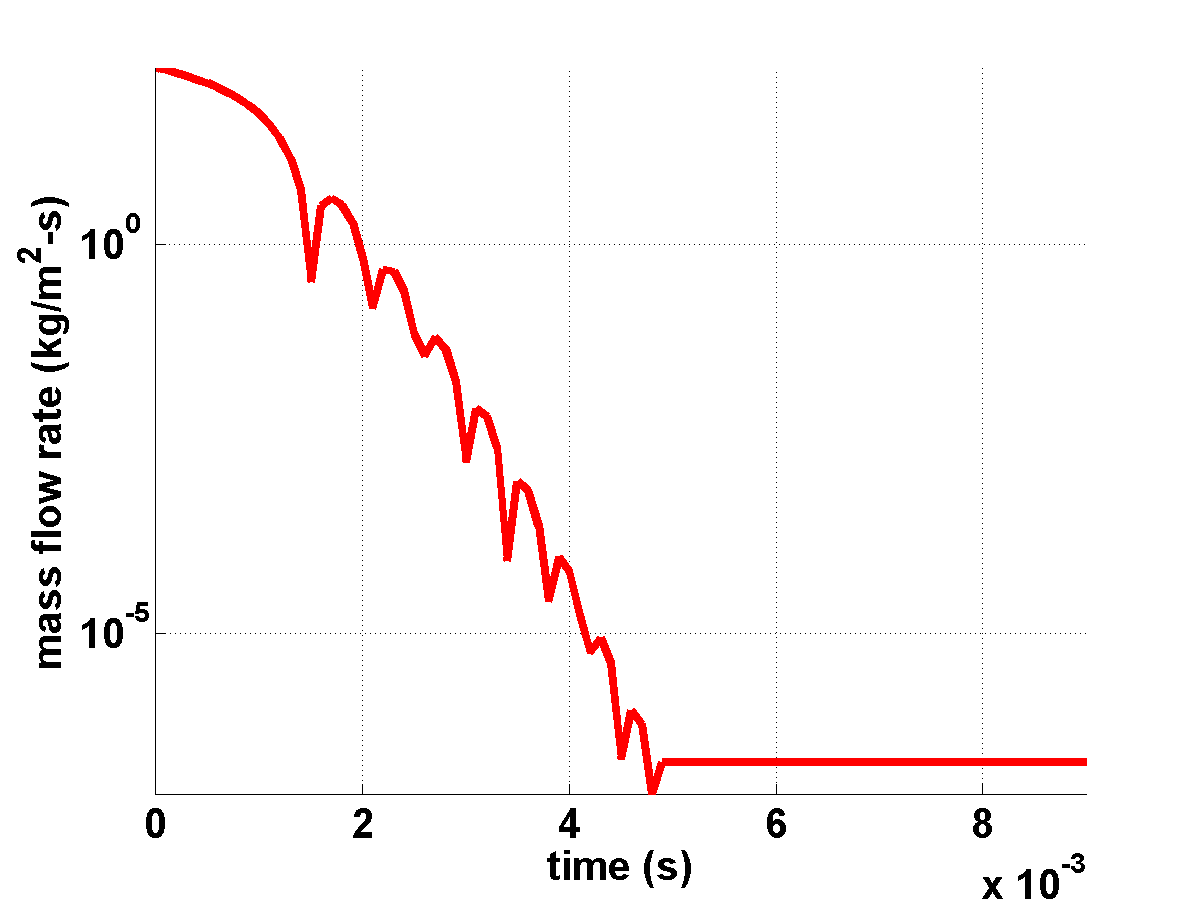
\includegraphics[scale=.50]{figures/CompressionCorner2DQ.png}
                \caption{Difference between inlet and outlet mass flow rates as a function of time.}
                \label{fig:2d_convergence}
        \end{figure}
%        \caption{Steady-state solution for a flow in a $2$-D compression corner.}\label{fig:2d_corner}
%\end{figure}
The steady-state numerical solution is given in \fig{fig:2d_corner}: the Mach number, the viscosity coefficients are plotted in \fig{fig:2d_corner_mach} and \fig{fig:2d_corner_visc}, respectively. The steady-state solution is formed of two regions of constant states, separated by the oblique shock. In \fig{fig:2d_corner_visc}, the viscosity coefficient is large in the shock, small anywhere else, and thus, behaves as expected. At the corner of the edge at $x=-0.25$ $m$, the viscosity coefficient is peaked because of the treatment of the wall boundary condition: at this particular node, the normal is not well defined and can cause numerical errors. The $1$-D plots of the pressure and the mach number at $y=0$, are also given in \fig{fig:2d_corner_isomach}: the shock does not show any spurious oscillations and is well resolved. Finally, the difference between the inlet and outlet mass flow rates is plotted in \fig{fig:2d_convergence} and show that the steady-state is reached. \\
Overall, the numerical solution does not show any oscillations, match the analytical solution, and the shock is well resolved.
%---------------------------------------------------------------------------------------------------
\subsection{Supersonic flow over a double wedge:} \label{sec:double_wedge}
%---------------------------------------------------------------------------------------------------
%---------------------------------------------------------------------------------------------------
\subsection{Supersonic flow over a forward facing step:} \label{sec:forward_facing_step}
%---------------------------------------------------------------------------------------------------
%%%%%%%%%%%%%%%%%%%%%%%%%%%%%%%%%%%%%%%%%%%%%%%%%%%%%%%%%%%%%%%%%%%%%%%%%%%%%%%%%%%%%%%%%%%%%%%%%%%%
%%%%%%%%%%%%%%%%%%%%%%%%%%%%%%%%%%%%%%%%%%%%%%%%%%%%%%%%%%%%%%%%%%%%%%%%%%%%%%%%%%%%%%%%%%%%%%%%%%%%
\section{Conclusions} \label{sec:ccl}
A new version of the entropy viscosity method valid for a wide range of Mach number and applied to the multi-D Euler equations with variable area was derived and presented. The definition of the viscosity coefficient is now consistent with the low Mach asymptotic limit, does not require an analytical expression of the entropy function, and thus, could be used with any equation of state having a convex entropy. Tests were performed with the Ideal and Stiffened Gas equation of states. In $1$-D, convergence of the numerical solution (either smooth or with shocks) to the exact solution was demonstrated by computing the convergence rates of the L$1$ and L$2$ norms of the error for flows in convergence-divergent nozzle and a straight pipe. $2$-D simulations were also performed for both subsonic and supersonic flows, and various geometries: the entropy viscosity method behaves well for a wide range of Mach number. The numerical results obtained for a flow over a circular bump (subsonic and transonic flows) illustrates the capabilities of the method to adapt to the flow type. \\
As future work, the entropy viscosity method will be extended to the $1$-D seven equations model \cite{SEM}. This two-phase flow system of equations is a good candidate for two reasons: it is unconditionally hyperbolic and degenerates to the multi-D Euler equations when one phase disappears.
%%%%%%%%%%%%%%%%%%%%%%%%%%%%%%%%%%%%%%%%%%%%%%%%%%%
%
%  New template code for TAMU Theses and Dissertations starting Fall 2012.  
%  For more info about this template or the 
%  TAMU LaTeX User's Group, see http://www.howdy.me/.
%
%  Author: Wendy Lynn Turner 
%	 Version 1.0 
%  Last updated 8/5/2012
%
%%%%%%%%%%%%%%%%%%%%%%%%%%%%%%%%%%%%%%%%%%%%%%%%%%%

%%%%%%%%%%%%%%%%%%%%%%%%%%%%%%%%%%%%%%%%%%%%%%%%%%%%%%%%%%%%%%%%%%%%%%
%%                           SECTION 4
%%%%%%%%%%%%%%%%%%%%%%%%%%%%%%%%%%%%%%%%%%%%%%%%%%%%%%%%%%%%%%%%%%%%%%

%%%%%%%%%%%%%%%%%%%%%%%%%%%%%%%%%%%%%%%%%%%%%%%%%%%%%%%%%%%%%%%%%%%%%%%
\chapter{\uppercase {Application of the entropy viscosity method to the seven-equation model}}\label{chap:seven}
%%%%%%%%%%%%%%%%%%%%%%%%%%%%%%%%%%%%%%%%%%%%%%%%%%%%%%%%%%%%%%%%%%%%%%
\tcr{seven-equation is an adjective to the noun model, so (1) it needs a hyphen and (2) it is ``singular'' since adjectives are invariable in English. Please check throughout the document.\\} \tcb{done}
%
Compressible two-phase flows are found in numerous industrial applications and thus have been an area of intense research in modeling and simulation over many years. A variety of models with different level of complexity has been developed such as: five-equation model \cite{Kapila_2001}\tcr{some each model you mention, provide some references}\tcr{regarding the 5-eq model, are there not several of them and not just one sch model? If so, say that and give more than one reference}, six-equation model \cite{Toumi_1996}, and more recently the seven-equation model \cite{SEM}. These models are all obtained by integrating the single-phase flow balance equations weighed by a characteristic function for each phase. The resulting system of equations contains non-conservative terms that describe the interaction between phases but also an equation for the volume fraction. Once a system of equations describing the physics is derived, the other challenging step is to develop a consistent numerical solver in order to obtain a numerical solution. Assuming that the system of equations is hyperbolic under some conditions, a Riemann solver could be used but is often ruled out because of the complexity due to the number of equations involved. Furthermore, careless approximation for the treatment of the non-conservative terms can lead to failure in computing the numerical solution \cite{Abgrall_2002}\tcr{a reference to back this up would be useful here} \tcb{done}. An alternative is to use an approximate Riemann solver, a well-established approach for single-phase flows, while deriving a consistent discretization scheme for the non-conservative terms. 

This methodology was applied to the seven-equation model (SEM) that was first introduced by Berry et al. in \cite{SEM}. This model is known to be unconditionally hyperbolic which is highly desirable when working with approximate Riemann solvers and can treat a wide range of applications. Its particularity comes from the pressure and velocity relaxation terms in the volume fraction, momentum and energy equations that can bring the two phases in equilibrium when using large values of the relaxation parameters. In other words, the seven-equation model can degenerate into the six and five equation models. Solving for the seven-equation model requires a numerical solver and a tremendous amount of work was dedicated to this task for spatially discontinuous schemes. Because each phase is assumed to obey the Euler equations, most of the numerical solvers are adapted from the single-phase approximate Riemann solvers. For example, Saurel et al. \cite{Saurel_2001a, Saurel_2001b} employed a HLL-type scheme to solve for the SEM but noted that excessive dissipation was added to the contact discontinuity. A more advanced HLLC-type scheme was developed in \cite{Li_2004} but only for the subsonic case and then extended to supersonic flows in \cite{Zein_2010}. More recently, Ambroso et al. \cite{Ambroso_2012} proposed an approximate Riemann solver accounting for source terms such as gravity and drag forces.\\

We propose to investigate how the EVM applies to the seven-equation model when discretized with a CFEM. First, the multi-D seven-equation model is recalled and detailed in \sect{sec:multi-seven-equ-model} and particular attention is given to the entropy equation. Then, the dissipative terms are derived using the entropy inequality, in \sect{sec:sev-equ-visc-reg-sect4}, on the same principle of what was done in \chap{chap:euler} for the multi-D Euler equations. In \sect{sec:sev-equ-visc-coeff-sect4}, a low-Mach asymptotic limit is performed in order to derive a definition for the viscosity coefficients consistent with the incompressible limit results. Lastly, 1-D numerical results are presented in \sect{sec:1d-num-res-sect4}.
%\begin{itemize}
%\item background on 7 emu model: first introduced. 
%\item method to solve this system: discontinuous scheme. Approximate Riemann solvers. Quote several papers
%\item differences between system of equation -> closure relations for relaxation coefficients.
%\end{itemize}

%===================================================================================
\section{Descriptions of the multi-D seven-equation model}\label{sec:multi-seven-equ-model}
%===================================================================================

The multi-D seven-equation model is obtained by assuming that each phase obeys the single-phase Euler equations (with phase-exchange terms) and by integrating over a control volume after multiplying by a characteristic function. The detailed derivation can be found in \cite{SEM}. In this section, the governing equations are recalled for each phase and the source terms are described. 
%-----------------------------------------------------------------------------------------
\subsection{The system of equations for the liquid and vapor phases}\label{sec:multi-d-7eqn-model-sect4}
%-----------------------------------------------------------------------------------------
The liquid phase obeys the following mass, momentum and energy balance equations, supplemented by a non-conservative volume-fraction equation:
%
\begin{subequations}\label{eq:liq-7-eqn-sect5}
\begin{align}
  % liquid mass conservation
  \label{multi-d-7-equ-liq}
  \frac{\partial \left( \alpha \rho \right)_{liq} A}{\partial t}
  + \div \left( \alpha \rho \mbold u \right)_{liq} A
  &= - \Gamma A_{int} A
\end{align}
\tcr{identity tensor missing in pressure term because you are using div and not grad} \tcb{ done}
\begin{align}
  % liquid momentum
  \frac{\partial \left( \alpha \rho \mbold u \right)_{liq} A}{\partial t}
  + \div \left[ \alpha_{liq} A \left( \rho \mbold u \otimes \mbold u + P \mathbb{I} \right)_{liq} \right]
  &= P_{int} A \grad \alpha_{liq} + P_{liq} \alpha_{liq} \grad A
    \nonumber
  \\
  &+ A \lambda_u (\mbold u_{vap} - \mbold u_{liq})
  - \Gamma A_{int} \mbold u_{int} A
\end{align}
\begin{align}
  % liquid total energy
  \frac{\partial \left( \alpha \rho E \right)_{liq} A}{\partial t}
  + \div \left[ \alpha_{liq} \mbold u_{liq} A \left( \rho E + P \right)_{liq} \right]
  &= P_{int} \mbold u_{int} A \grad \alpha_{liq} - \bar{p}_{int} A \mu_P (P_{liq} - P_{vap})
        \nonumber
  \\
  + \bar{\mbold u}_{int} A \lambda_u (\mbold u_{vap} - \mbold u_{liq})
&  + \Gamma A_{int} \left( \frac{p_{int}}{\rho_{int}} - H_{liq, int} \right) A
\end{align}
\begin{align}
  % liquid volume fraction
  \label{eqn:multi-d-7-eqn-liq-vol}
  \frac{\partial \alpha_{liq} A}{\partial t} + A\mbold u_{int} \cdot \grad \alpha_{liq}
  &= A \mu_P (P_{liq} - P_{vap}) - \frac{\Gamma A_{int} A}{\rho_{int}}
\end{align}
\end{subequations}
%
On the same model, the equations for the vapor phase are:
%
\begin{subequations}\label{eq:vap-7-eqn-sect5}
\begin{align}
  \label{multi-d-7-equ-vap}
  % vapor mass conservation
  \frac{\partial \left( \alpha \rho \right)_{vap} A}{\partial t}
  + \div \left( \alpha \rho \mbold u \right)_{vap} A
  =  \Gamma A_{int} A
\end{align}
\begin{align}
  % vapor momentum
  \frac{\partial \left( \alpha \rho u \right)_{vap} A}{\partial t}
  + \div \left[ \alpha_{vap} A \left( \rho \mbold u \otimes \mbold u + P\mathbb{I} \right)_{vap} \right]
  &= P_{int} A \grad \alpha_{vap} + P_{vap} \alpha_{vap} \grad A
  \\
  \nonumber
  &+ A \lambda_u (\mbold u_{liq} - \mbold u_{vap})
  + \Gamma A_{int} u_{int} A
\end{align}
\begin{align}
  % vapor total energy
  \frac{\partial \left( \alpha \rho E \right)_{vap} A}{\partial t}
  &+ \div \left[ \alpha_{vap} \mbold u_{vap} A \left( \rho E + P \right)_{vap} \right]
  = P_{int} \mbold u_{int} A \grad \alpha_{vap} - \bar{P}_{int} A \mu_P (P_{vap} - P_{liq})
  \\
  \nonumber
  &+ \bar{\mbold u}_{int} A \lambda_u (\mbold u_{liq} - \mbold u_{vap})
- \Gamma A_{int} \left( \frac{p_{int}}{\rho_{int}} - H_{vap, int} \right) A
\end{align}
\begin{align}
  % vapor phase volume fraction
  \label{eqn:multi-d-7-eqn-vap-vol}
  \frac{\partial \alpha_{vap} A}{\partial t} + A \mbold u_{int} \cdot \grad \alpha_{vap}
  &= A \mu_P (P_{vap} - P_{liq}) + \frac{\Gamma A_{int} A}{\rho_{int}}
\end{align}
\end{subequations}
%
where $\alpha_k$, $\rho_k$, $\mbold u_k$ and $E_k$ denote the volume fraction, the density, the velocity vector and the total specific energy of phase $k=\left\{ liq, vap \right\}$, respectively. The phase pressure $P_k$ is computed from an equation of state. The interfacial variables are denoted by the subscript $int$ and their definition will be given in \sect{sec:source-terms-7-eqt-sect5}. The interfacial pressure and velocity and their corresponding average values are denoted by $P_{int}$, $\mbold u_{int}$, $\bar{P}_{int}$ and $\bar{\mbold u}_{int}$, respectively. $\Gamma$ is the net mass transfer per unit interfacial area from the liquid to the vapor phase and $A_{int}$ is the interfacial area per unit volume of mixture.  Also, $H_{liq, int}$ and $H_{vap, int}$ are the liquid and gas total specific enthalpies at the interface, respectively. $\mu_P$ is the pressure relaxation coefficient and $\lambda_u$ denotes the velocity relaxation coefficient. Lastly, the cross section $A$ is only spatially dependent. In the case of two-phase flows, the equation for the vapor volume fraction, \eqt{eqn:multi-d-7-eqn-vap-vol}, is simply replaced by the algebraic relation
%
\begin{align}
 \alpha_{vap}= 1 - \alpha_{liq}
\end{align}
%
The set of eight equations given in \eqt{eq:liq-7-eqn-sect5} and in \eqt{eq:vap-7-eqn-sect5} is now reduced to seven which yields the multi-D seven-equation model. A set of seven waves is present in such a model: two acoustic waves and a contact wave for each phase supplanted by a volume fraction wave propagating at the interface velocity $\mbold u_{int}$. Considering a domain of dimension $\mathbb{D}$, the corresponding eigenvalues are the following for each phase $k$:
% 
\begin{align}
&\lambda_1 = \mbold u_{int} \nonumber\\
&\lambda_{2,k} = \mbold u_k \cdot \mbold n - c_k \nonumber\\
&\lambda_{3,k} = \mbold u_k \cdot \mbold n + c_k \nonumber\\
&\lambda_{d+3,k} = \mbold u_k \cdot \mbold n \text{ for } d = 1 \dots \mathbb{D},\nonumber
\end{align}
%
where $\mbold n$ is a unit vector pointing to a given direction.\tcr{not sure random is correct here!} \tcb{ done } \\
For each phase $k$, an entropy equation can be derived when accounting only for the pressure and velocity relaxation terms (all of the terms proportional to the net mass transfer term $\Gamma$ are removed). The entropy function for a phase $k$ is denoted by $s_k$ and function of the density $\rho_k$ and the internal energy $e_k$. The derivation is detailed in \app{app:sev-equ-model-entropy} and only the final result is recalled here:
%
\begin{align}\label{eq:ent-eqn-7-eqn-model}
(s_{e})_k^{-1} \alpha_k \rho_k A \frac{Ds_k}{Dt} &= \mu_P \frac{Z_k}{Z_k+Z_j} (P_j - P_k)^2 + \lambda_u \frac{Z_j}{Z_k+Z_j} (\mbold u_j -\mbold  u_k)^2 \nonumber
\\
& \frac{Z_k}{\left( Z_k+Z_j \right)^2} \left[ Z_j (\mbold u_j-\mbold u_k)+\frac{\grad \alpha_k}{|| \grad \alpha_k ||}(P_k-P_j)\right]^2,
\end{align}
where $Z_{k}$ denotes the phasic acoustic impedance and is defined as the product of the density and the speed of sound: $Z_k = \rho_k c_k$. The partial derivative of the entropy function $s_k$ with respect to the internal energy $e$, $(s_e)_k$, is defined proportional to the inverse of the temperature of phase $k$ alike in \chap{chap:euler} for the single phase Euler equations. The right hand-side of \eqt{eq:ent-eqn-7-eqn-model} is unconditionally positive since all terms are squared. Furthermore, \eqt{eq:ent-eqn-7-eqn-model} is valid for each phase $k=\left\{liq, vap \right\}$ and ensures positivity of the total entropy equation that is obtained by summing over the phases:
%
\begin{equation}\label{eq:tot-ent-res-sct4}
\sum_k (s_{e})_k^{-1} \alpha_k \rho_k A \frac{Ds_k}{Dt} = \sum_k (s_{e})_k^{-1} \alpha_k \rho_k A \left( \partial_t s_k + \mbold u_k \cdot \grad s_k \right) \geq 0.
\end{equation}
%
Note that when one phase disappears, \eqt{eq:tot-ent-res-sct4} degenerates into the single phase entropy equation given in \eqt{eq:ent_res}.
%\begin{itemize}
%\item give system of equation with relaxation terms and mass transfer term from DEM paper
%\item explain the relaxation terms
%\item explain the source terms: exchanges between phases.
%\item entropie equation.
%\end{itemize}
%-----------------------------------------------------------------------------------------
\subsection{The source terms}\label{sec:source-terms-7-eqt-sect5}
%-----------------------------------------------------------------------------------------
In this section, insights about the relaxation terms, the net mass transfer term and the interfacial heat transfer terms are given.
%---------------------------------------------------------------------------------------------------------------
\subsubsection{Interface Pressure and Velocity, Mechanical Relaxation Coefficients}
%---------------------------------------------------------------------------------------------------------------
The relaxation terms are used to bring the two phases in equilibrium by making pressure and velocity equal. The mechanical relaxation coefficients $\mu_P$ and $\lambda_u$ can be seen as inverse relaxation times \tcr{it feels more like inverse times} \tcb{done}: the larger the relaxation coefficients, the faster the two phases will be brought to equilibrium. Derivation of the relaxation terms is achieved by using rational thermodynamic to ensure consistency with the second thermodynamic law \cite{Truesdell}. The methodology is very similar to what is done for the derivation of the dissipative terms using the entropy inequality.

In the continuous limit of small mesh spacing and time steps along with employment of the Godunov weak wave limit, it can be shown that the pressure and velocity relaxation terms obeys the following relations \cite{Berry_2008b, Chinnayya_2004}:
%
\begin{align}
  \label{E-R:83}
  p_{int} &= \bar{p}_{int} + \frac{Z_{liq}Z_{vap}}{Z_{liq}+Z_{vap}} \frac{\grad \alpha_{liq}}{|| \grad \alpha_{liq} ||} \cdot (\mbold u_{vap}-\mbold u_{liq})
  \\
  \bar{p}_{int} &= \frac{Z_{vap}p_{liq}+Z_{liq}p_{vap}}{Z_{liq}+Z_{vap}}
\end{align}
%
The interfacial velocities $\mbold u_{int}$ and its average value $\bar{\mbold u}_{int}$ are computed from:
%
\begin{align}
  \label{E-R:84}
  \mbold u_{int} &= \bar{\mbold u}_{int} +  \frac{\grad \alpha_{liq}}{|| \grad \alpha_{liq} ||} \frac{p_{vap}-p_{liq}}{Z_{liq}+Z_{vap}}
  \\
  \bar{\mbold u}_{int} &= \frac{Z_{liq} \mbold u_{liq}+Z_{vap}\mbold u_{vap}}{Z_{liq}+Z_{vap}}.
\end{align}
%
The pressure, $\mu_P$, and velocity, $\lambda_u$, relaxation coefficients are proportional to each other and function of the interfacial area $A_{int}$:
%
\begin{align}
  \label{E-R:85}
  \lambda_u &= \frac{1}{2} \mu_P Z_{liq} Z_{vap}
  \\
  \label{E-R:86}
  \mu_P &= \frac{A_{int}}{Z_{liq}+Z_{vap}}
\end{align}
%where $\lambda_u$ is the velocity relaxation coefficient function, $\mu_P$
%is the pressure relaxation coefficient function, $Z_k = \rho_k c_k$,
%$(k=liq, vap)$, is the phasic acoustic impedance and 
The specific interfacial area (i.e., the interfacial surface area per unit
volume of two-phase mixture), $A_{int}$, must be specified from some type of
flow regime map or function. In \cite{SEM}, it is chosen to be a function of the liquid volume fraction:
%
\begin{equation}\label{eq:Aint-sect4}
A_{int} = A_{int}^{max} \left[ 6.75 \left(1-\alpha_{liq} \right)^2 \alpha_{liq} \right],
\end{equation}
% 
\tcr{is a square missing above?} \tcb{ nope }
where $A_{int}^{max} = 5100$ $m^2 / m^3$. With such definition, the interfacial area is zero in the limits $\alpha_{liq} = 0$ and $\alpha_{liq} = 1$. 
%The DEM model for two-phase flow of
%water and its vapor in a one dimensional duct of spatially varying
%cross-section was derived and demonstrated with these closures by
%Berry et al.~\cite{SEM}.
%From this specification for $\lambda_u$ and $\mu_P$ it is clear
%that special coupling is rendered\tcr{???}.  
To relax the seven-equation model to
the ill-posed classical six-equation model, the pressures should be
relaxed toward a single pressure for both phases.  This is
accomplished by specifying the pressure relaxation coefficient to be
very large, i.e., letting it approach infinity.  But if the pressure
relaxation coefficient goes to infinity, so does the velocity
relaxation rate also approach infinity.  This then relaxes the
seven-equation model not to the classical six equation model but to the
mechanical equilibrium five equation model of Kapila \cite{Kapila_2001}.  This reduced
five equation model is also hyperbolic and well-posed. The five equation
model provides a very useful starting point for constructing
multi-dimensional interface resolving methods which dynamically
captures evolving and spontaneously generated
interfaces~\cite{Saurel_2009}. Thus the seven-equation model
can be relaxed locally to couple seamlessly with such a
multi-dimensional, interface resolving code.

Numerically, the mechanical relaxation coefficients $\mu_P$
(pressure) and $\lambda_u$ (velocity) can be relaxed independently to
yield solutions to useful, reduced models (as explained previously).  It
is noted, however, that relaxation of pressure only by making $\mu_P$
large without relaxing velocity will indeed give ill-posed and
unstable numerical solutions, just as the classical six equation
two-phase model does, with sufficiently fine spatial resolution, as
confirmed in~\cite{SEM,Herrard_2005}.

Even though the implementation of the seven equation two-phase
model does not use
the generalized approach of DEM, the interfacial pressure and velocity
closures as well as the pressure and velocity relaxation coefficients
of Equations~\eqref{E-R:83} to~\eqref{E-R:86} are utilized.
%-----------------------------------------------------------------------------------------
\subsubsection{Interphase Mass Transfer}
%-----------------------------------------------------------------------------------------
For vapor to be formed from the liquid phase (vaporization) energy
must be added to the liquid to produce vapor at nucleation sites;
whether the liquid is heated directly or decompressed below its
saturation pressure.  A liquid to vapor phase change may occur based
on two main mechanisms.  The first is related to vaporization induced
by external heating or heat transfer in a nearly constant pressure
environment which is called heterogeneous boiling, or simply
boiling.  This heat input can occur through a solid/liquid
interface with the solid typically hotter than the liquid, or through
a liquid/gas interface with the gas being hotter than the liquid.

\begin{figure}
  \centering
  %\fbox{
   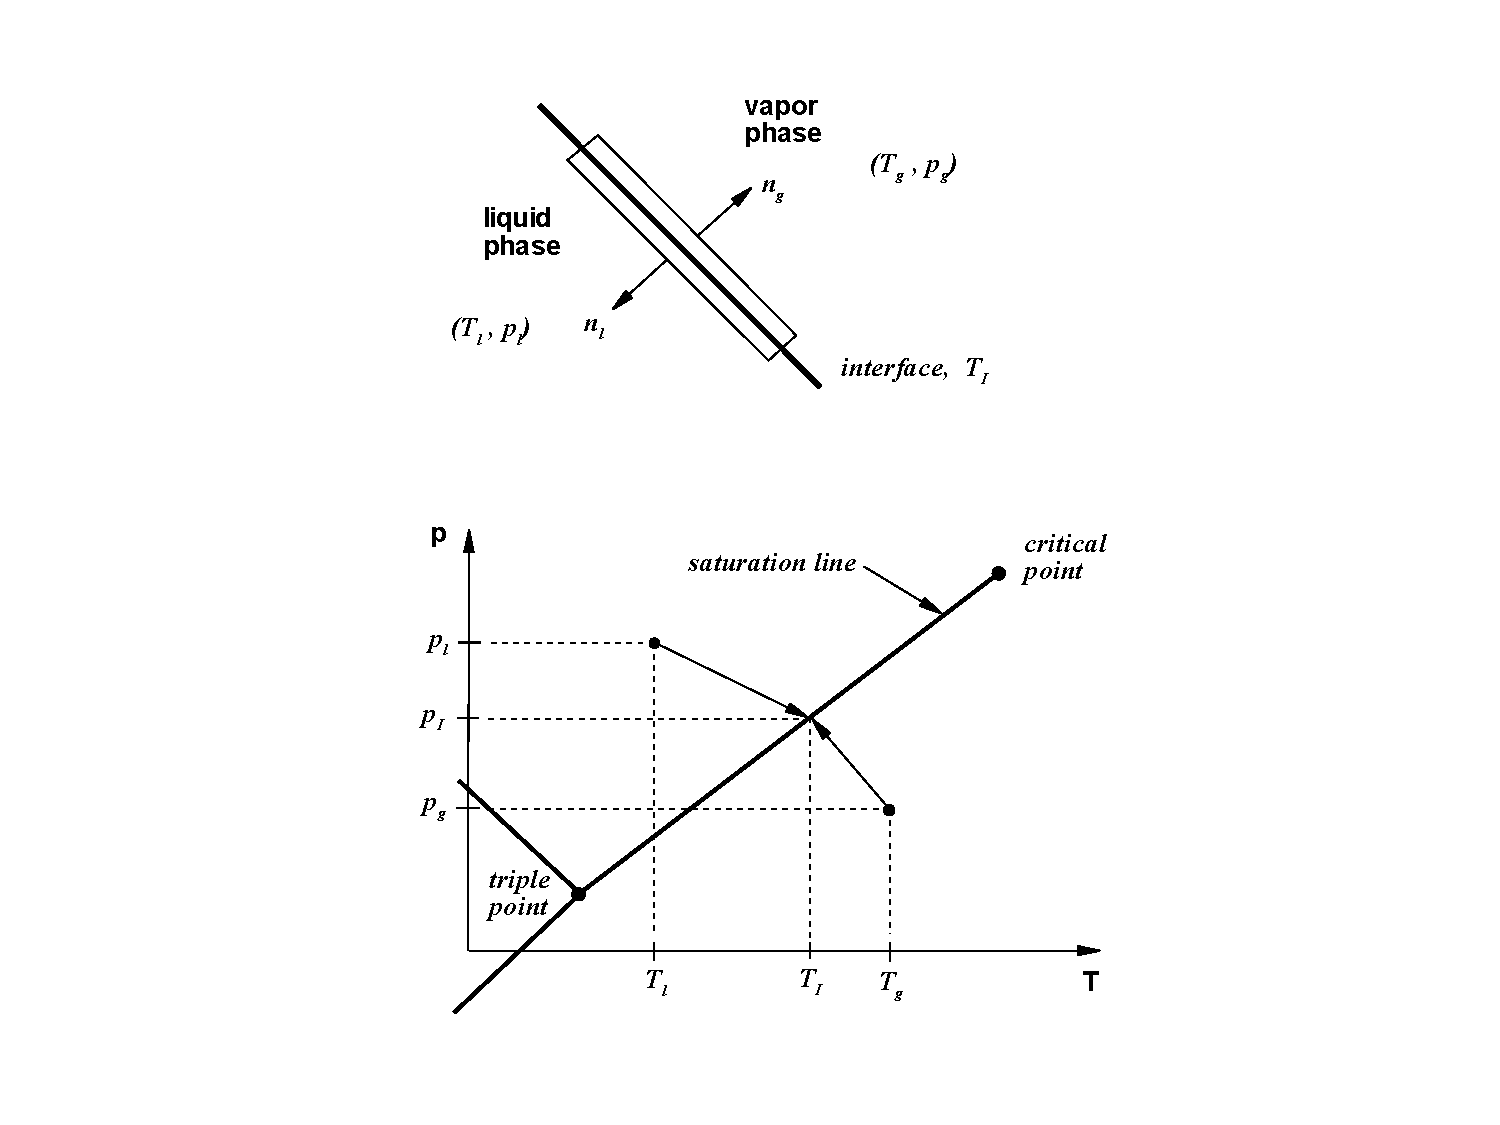
\includegraphics[clip=true,viewport=200 50 550 500,width=.8\textwidth]{figures/SEM/saturation}
   % }
   \caption{Interface control volume (top); $T$-$p$ state space around
     saturation line, $T_{liq} < T_{vap}$, (bottom).\label{Berry-Fig:2}}
\end{figure}

To examine the mass flow rate between phases, local mechanisms of the
vaporization (condensation) process are considered between the liquid
phase and its associated vapor in the presence of temperature
gradients.  The mechanisms of interest here are dominated by heat
diffusion at the interface.  The pertinent local equations to consider
are the mass and energy equations.  As a vaporization front propagates
slowly (on the order of 1 mm/s to 1 m/s) compared to acoustic waves
present in the medium (which propagate with speeds of the order 1
km/s), acoustic propagation results in quasi-isobaric pressure
evolution through vaporization fronts.  The momentum equation is
therefore not needed -- because the quasi-isobaric assumption
(neglecting the pressure and kinetic energy variations in the total
energy equation) is made.  A simple expression for the interphase
mass flow rate is obtained
\begin{align}
  \nonumber
  \Gamma = \Gamma_{vap}
  &= \frac{h_{T,  liq} \left( T_{liq} - T_{int} \right) + h_{T,  vap} \left( T_{vap} - T_{int} \right)}{h_{vap,  int} - h_{liq,  int}}
  \\
  &= \frac{h_{T,  liq} \left( T_{liq} - T_{int} \right) + h_{T,  vap} \left( T_{vap} - T_{int} \right)}{L_v \left( T_{int} \right)}
\end{align}
where $L_v \left( T_{int} \right) = h_{vap,  int} - h_{liq,  int}$
represents the latent heat of vaporization.  The interface
temperature is determined by the saturation constraint
$T_{int}=T_{sat}(p)$ with the appropriate pressure $p=\bar{p}_{int}$
determined above, the interphase mass flow rate is thus determined.
The lower graphic of Figure~\ref{Berry-Fig:2} schematically shows the
$p$-$T$ state space in the vicinity of the saturation line (shown
for the case with $T_{liq} < T_{vap}$).

To better illustrate the model for vaporization or condensation,
Figure~\ref{Berry-Fig:3} shows pure liquid and pure vapor regions
separated by an interface.
\begin{figure}
  \centering
  %\fbox{
   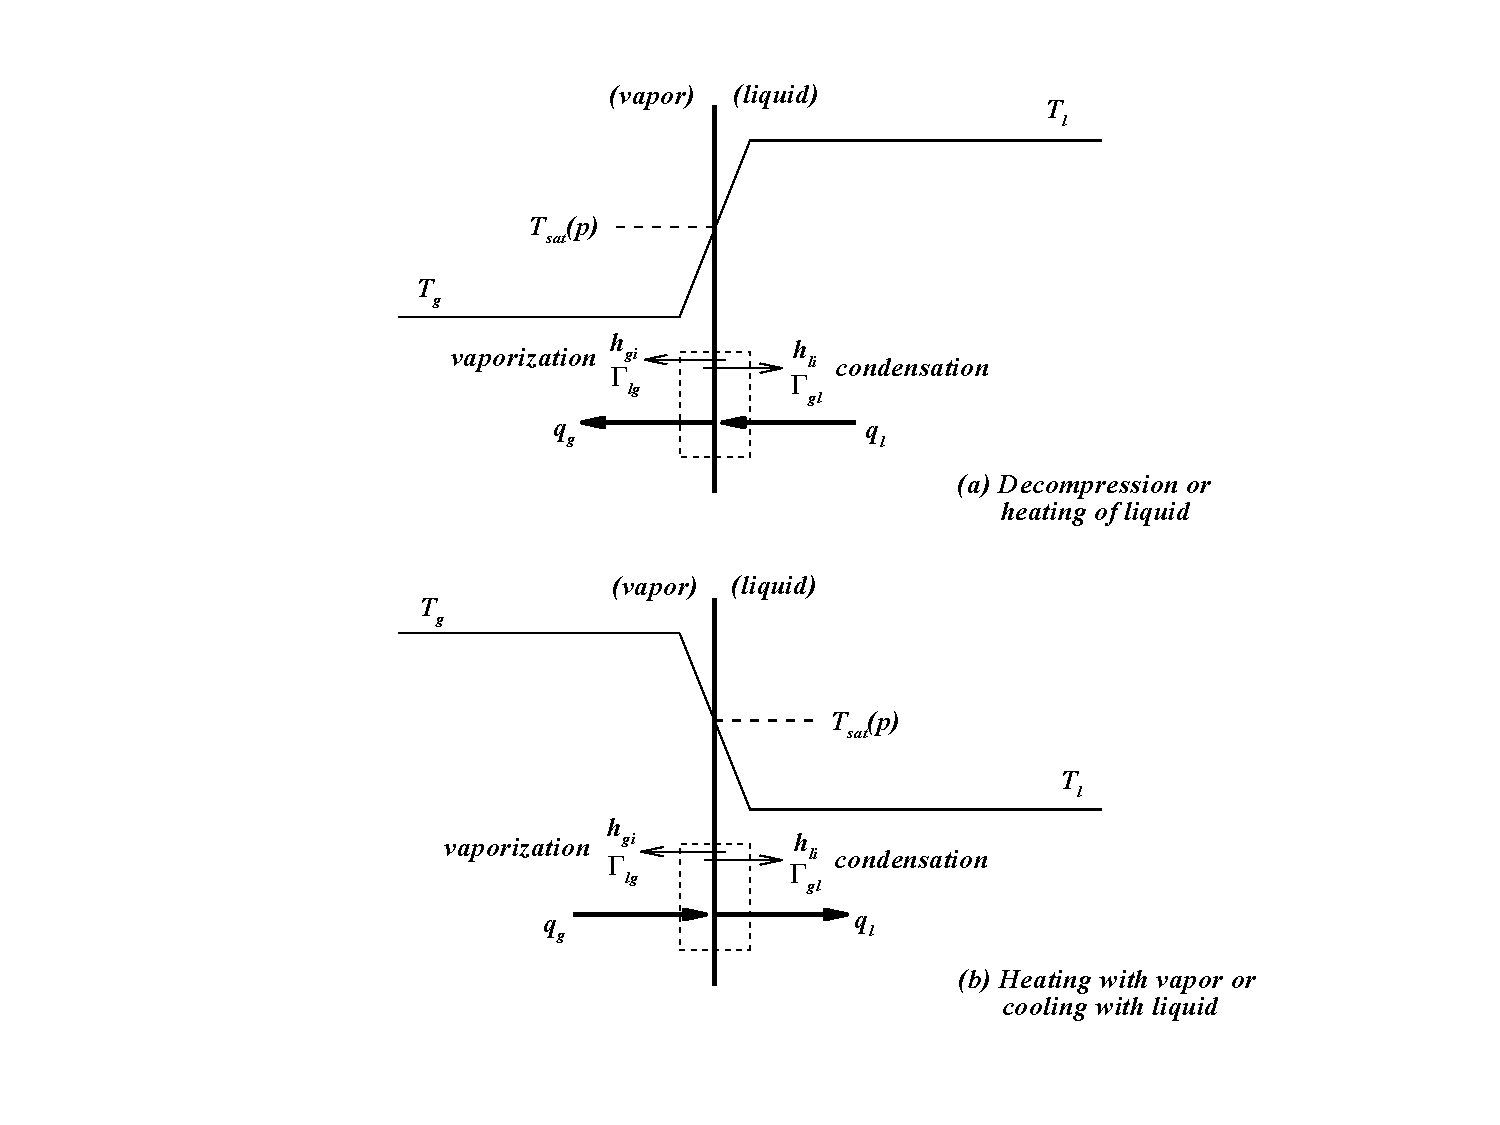
\includegraphics[clip=true,viewport=175 50 625 525,width=.8\textwidth]{figures/SEM/vaporization_condensation}
 %}
   \caption{Vaporization and condensation at a liquid-vapor interface
     (after Moody~\cite{Moody_1990}).\label{Berry-Fig:3}}
\end{figure}
Representative temperature profiles are shown for heat transfer from
vapor to liquid or liquid to vapor.  As discussed by
Moody~\cite{Moody_1990}, either vaporization or condensation can occur
for both temperature profiles. The interphase mass transfer is
determined by the net interfacial heat transfer: if net heat transfer
is toward the interface, vapor will form; conversely, if net heat
transfer is away from the interface, liquid will condense.
Figure~\ref{Berry-Fig:3} shows heat transfer rates $q_{vap}$ and
$q_{liq}$ from the vapor and liquid sides of the interface.  For
bidirectional phase change (vaporization and condensation), mass
transfer based on heat balance at the interface is adopted.  When
vaporization occurs, vapor is assumed to form at a saturated interface
temperature $T_{int}=T_{sat}(\bar{p}_{int})$.  If condensation occurs,
liquid is assumed to form also at a saturated interface temperature
$T_{int}=T_{sat}(\bar{p}_{int})$.  The interfacial total enthalpies
correspond to the saturated values in order that the interphase mass
transfer rate and conservation of total energy be compatible:
\begin{equation}
  \label{E-R:95}
  H_{k,  int} = h_{k,  int} + \frac{1}{2} u_{int}^2
\end{equation}
for phase $k=(liq, vap)$, where $h_{k,int}$ \tcr{h int not defined} \tcb{I am not sure} is the phase $k$ specific enthalpy
evaluated at the interface condition.  Phasic specific enthalpy
depends upon the equation of state used and will be discussed with the
equations of state.  The interfacial density corresponds to the liquid
saturated density $\rho_{int} = \rho_{liq, sat}(p_{int})$.\tcr{not pbar int?} \tcb{not in the latest version}
%-----------------------------------------------------------------------------------------
\subsubsection{Interface Direct Heat Transfer}
%-----------------------------------------------------------------------------------------
Without wall boiling, a simple model for the direct, convective heat transfer
from the wall to fluid phase $k$ will be the same as that of a single-phase
except the duct wall area over which this heat transfer can occur is weighted
by the wetted fraction of the phase.  That is,
\begin{equation}
  Q_{ \text{wall}, k } = H_{w,k} a_w \left(T_k  - T_{ \text{wall} } \right) \alpha_k A
\end{equation}
\tcr{aw not defined} \tcb{ done}
for phase $k=(liq, vap)$, where $H_{w,k}$ is the wall convective wall heat transfer
coefficient associated with phase $k$ and $a_w$ is the wall-heated surface. Similarly, the direct heat
transfer from/to the interface to/from the phase $k$, which will also
be used to determine the mass transfer between the phases, is
\begin{equation}
  Q_{int,  k} = h_{T,  k}  \left( T_{int} - T_k \right)  A_{int}  A
\end{equation}
with $h_{T,  k}$ denoting the convective heat transfer coefficient
between the interface and phase $k$. The phasic bulk
temperature $T_k$ is determined from the respective phase's equation of
state.
%-----------------------------------------------------------------------------------------
\subsubsection{Stiffened Gas Equation of State for Two-phase Flows} \label{sec:SGEOS}
%-----------------------------------------------------------------------------------------
With the seven equation two-phase model each phase is compressible and
behaves with its own convex equation of state (EOS).  For initial
development purposes it was decided to use a simple form capable of
capturing the essential physics.  For this purpose the stiffened
gas equation of state (SGEOS)~\cite{SGEOS} was selected (as
it was also for single phase)
\begin{equation}
  \label{E-R:96}
  p(\rho,e) = (\gamma -1) \rho (e - q) - \gamma p_{\infty}
\end{equation}
where $p$, $\rho$, $e$, and $q$ are the pressure, density,
internal energy, and the binding energy of the fluid considered.  The
parameters $\gamma$, $q$, and $p_{\infty}$ are the constants
(coefficients) of each fluid.  The first term on the right hand side
is a repulsive effect that is present for any state (gas, liquid, or
solid), and is due to molecular vibrations.  The second term on the
right represents the attractive molecular effect that guarantees the
cohesion of matter in the liquid or solid phases.  The parameters used
in this SGEOS are determined by using a reference curve, usually in
the $\left(p, \frac{1}{\rho}\right)$ plane.

To extend this equation of state for two phases,
LeMetayer~\cite{SGEOS} uses the saturation curves as this
reference curve to determine the stiffened gas parameters for liquid
and vapor phases.  The SGEOS is the simplest prototype that contains
the main physical properties of pure fluids, repulsive and attractive
molecular effects, thereby facilitating the handling of the essential
physics and thermodynamics with a simple analytical formulation.  Thus
each fluid has its own thermodynamics.  For each phase the
thermodynamic state is determined by the SGEOS:
\begin{align}
  \label{E-R:97}
  e(p,\rho) &= \frac{p+\gamma p_{\infty}}{(\gamma -1) \rho} + q
  \\
  \label{E-R:98}
  \rho (p,T) &= \frac{p+p_{\infty}}{(\gamma -1) c_v T}
  \\
  \label{E-R:99}
  h(T) &= \gamma  c_v T + q
  \\
  \label{E-R:100}
  g(p,T) &= \left(\gamma c_v - q'\right) T - c_v T \ln \frac{T^\gamma}{\left(p+p_{\infty}\right)^{\gamma-1}} + q
\end{align}
where $T$, $h$, and $g$ are the temperature, enthalpy,
and Gibbs free enthalpy, respectively, of the phase considered.  In
addition to the three material constants mentioned above, two
additional material constants have been introduced, the constant
volume specific heat $c_v$ and the parameter $q'$.  The method to
determine these parameters in liquid-vapor systems, and in particular
the coupling of liquid and vapor parameters, is given
in~\cite{SGEOS}.  The values for water and its vapor from that
reference are given in Table 2.  These parameter values appear to
yield reasonable approximations over a temperature range from 298K to
473K.  For higher temperature range the parameters can easily be
refit.

Unlike van der Waals type modeling where mass transfer is a
thermodynamic path, with the seven equation two-phase model the mass
transfer modeling, which produces a relaxation toward thermodynamic
equilibrium, is achieved by a kinetic process.  Thus the seven equation
model preserves hyperbolicity during mass transfer.
From equation~\eqref{E-R:99} it is readily seen that the phase
$k$ specific enthalpy evaluated at the interface condition from
equation~\eqref{E-R:95} is
\begin{equation}
  h_{k,  int} = c_{p, k}  T_{int} + q_k
\end{equation}
because $c_{p, k} = \gamma_k  c_{v, k}$.

The bulk interphase mass transfer from the liquid phase to the vapor
phase $\Gamma$ is due to their difference in Gibb's free energy.  At
saturated conditions the Gibb's energies of the two-phases are equal.
It is necessary to determine the saturation temperature $T_{sat}(p)$
for given pressure $p=\bar{p}_{int}$ and the heat of vaporization
$L_v\left(T_{sat}(\bar{p}_{int}) \right)$ at this saturation temperature
with the SGEOS for each phase.  For this calculation, the procedure
of~\cite{SGEOS} is adopted.  This procedure for the
determination of SGEOS parameters can be made very accurate provided
the two reference states are picked sufficiently close to represent
the experimental saturation curves as locally quasi-linear.
Restrictions occur near the critical point, but away from this point
wide ranges of temperatures and pressures can be considered.  At
thermodynamic equilibrium at the interface, the two phasic Gibbs free
enthalpies must be equal, $g_{vap}=g_{liq}$, so the use of equation~\eqref{E-R:100}
yields
\begin{equation}
  \label{E-R:102}
  \ln \left( p + p_{\infty,  vap} \right) = A + \frac{B}{T} + C  \ln(T) + D  \ln \left( p + p_{\infty,  liq} \right)
\end{equation}
where
\begin{align}
  A &= \frac{c_{p, liq} - c_{p, vap} + q'_{vap} - q'_{liq}}{c_{p,  vap} - c_{v,  vap}} \\
  B &= \frac{q_{liq}-q_{vap}}{c_{p,  vap} - c_{v,  vap}} \\
  C &= \frac{c_{p, vap} - c_{p, liq}}{c_{p,  vap} - c_{v,  vap}} \\
  D &= \frac{c_{p, liq} - c_{v, liq}}{c_{p,  vap} - c_{v,  vap}} \,\,.
\end{align}
Relation~\eqref{E-R:102} is nonlinear, but can used to compute the
theoretical curve $T_{sat}(p)$.  A simple Newton iterative numerical
procedure is used.  With $T_{sat}(p)$ determined, the heat of
vaporization is calculated as
\begin{align}
  \nonumber
  L_v \left( T_{int} \right) &= h_{vap,  int} - h_{liq,  int}
  \\
  \nonumber
  &= h_{k,  int}
  \\
  &= \left( \gamma_{vap}  c_{v, vap}  T + q_{vap} \right) - \left( \gamma_{liq}  c_{v, liq}  T + q_{liq} \right) \,.
\end{align}
%
%===================================================================================
\section{A viscous regularization for the multi-D seven-equation model}\label{sec:sev-equ-visc-reg-sect4}
%===================================================================================
In this section, the dissipative terms for the multi-D seven-equation model \emph{with pressure and velocity relaxation source terms} are derived. The methodology proposed in  \chap{chap:theory_chp1} is followed. For clarity purpose, the seven-equation model with pressure and velocity relaxation terms is recalled when considering a phase $k$ in interaction with a second phase $j$:
%
\tcr{below, you have dropped the P subscript for mu, and the u subscript for lambda} \tcb{ done }
\begin{subequations}\label{eq:sev_equ}
\begin{align}
\partial_t \left( \alpha_k  A\right) + \mbold u_{int} A \grad \alpha_k = A \mu_P \left( P_k - P_j \right)
\end{align}
\begin{align}
\partial_t \left( \alpha_k \rho_k A \right) + \div \left( \alpha_k \rho_k \mbold u_k A \right) = 0
\end{align}
\begin{align}
\partial_t \left( \alpha_k \rho_k u_k A \right) + \div \left[ \alpha_k A \left( \rho_k \mbold u_k \otimes \mbold u_k + P_k \mathbb{I} \right) \right] &=\nonumber\\
\alpha_k P_k \grad A + P_{int} A \grad \alpha_k &+ A \lambda_u \left( \mbold u_j - \mbold u_k \right)
\end{align}
\begin{align}
\partial_t \left( \alpha_k \rho_k E_k A \right) + \div \left[ \alpha_k A \mbold u_k \left( \rho_k E_k + P_k \right) \right] &=\nonumber\\
P_{int} \mbold u_{int} A \grad \alpha_k - \mu_P \bar{P}_{int} \left( P_k-P_j \right) &+ \bar{\mbold u}_{int}A \lambda_u \left( \mbold u_j - \mbold u_k \right)
\end{align}
\end{subequations}
%
%where $\rho_k$, $u_k$, $E_k$ and $P_k$ are the density, the velocity, the specific total energy and the pressure of $k^{th}$ phase, respectively. The pressure and velocity relaxation parameters are denoted by $\mu$ and $\lambda$, respectively. The variables with index $_I$ correspond to the interfacial variables and a definition for those can be found in \cite{SEM}. The cross-section $A$ is only function of space: $\partial_t A = 0$.
In order to apply the EVM, dissipative terms are added to each equation of the system given in \eqt{eq:sev_equ}, which yields:
%
\begin{subequations}\label{eq:sev_equ-with-diss-terms}
\begin{align}\label{eq:sev_equ-with-diss-terms-vf}
\partial_t \left( \alpha_k  A\right) + \mbold u_{int} A \grad \alpha_k = A \mu_P \left( P_k - P_j \right) + \div \mbold l_k
\end{align}
\begin{align}\label{eq:sev_equ-with-diss-terms-cont}
\partial_t \left( \alpha_k \rho_k A \right) + \div \left( \alpha_k \rho_k \mbold u_k A \right) = \div \mbold f_k
\end{align}
\begin{align}\label{eq:sev_equ-with-diss-terms-mom}
\partial_t \left( \alpha_k \rho_k \mbold u_k A \right) + \div \left[ \alpha_k A \left( \rho_k \mbold u_k \otimes \mbold u_k + P_k \mathbb{I} \right) \right] &=\nonumber\\
\alpha_k P_k \grad A + P_{int} A \grad \alpha_k &+ A \lambda_u \left( \mbold u_j - \mbold u_k \right) + \div \mbold g_k
\end{align}
\begin{align}\label{eq:sev_equ-with-diss-terms-ener}
\partial_t \left( \alpha_k \rho_k E_k A \right) + \div \left[ \alpha_k A \mbold u_k \left( \rho_k E_k + P_k \right) \right] &=\nonumber\\
P_{int} \mbold u_{int} A \grad \alpha_k - \mu_P \bar{P}_{int} \left( P_k-P_j \right) &+ \bar{\mbold u}_{int}A \lambda_u \left( \mbold u_j - \mbold u_k \right) + \div \left( \mbold h_k + \mbold u \cdot \mbold g_k \right)
\end{align}
\end{subequations}
%
where $\mbold f_k$, $\mbold g_k$, $\mbold h_k$ and $\mbold l_k$ are the dissipative terms. The next step consists of deriving the entropy equation for the phase $k$, on the same model as what is done in \app{app:sev-equ-model-entropy}. Extra terms will appear in the right-hand-side of the entropy equation due to the dissipative terms. By choosing properly the definition of the dissipative terms, the sign of these extra terms can be controlled in order to ensure positivity of the entropy residual:
%
\begin{enumerate}
\item recast the system of equation given in \eqt{eq:sev_equ-with-diss-terms} in terms of the primitive variables $(\alpha_k, \rho_k, \mbold u_k, e_k)$.
\item derive the entropy equation by using the chain rule:
\begin{equation}
\label{eq:chain_rule-sct4}
\frac{Ds_k}{Dt} = \left( s_{\rho} \right)_k \frac{D \rho_k}{Dt} + \left( s_{e} \right)_k \frac{D e_k}{Dt} 
\end{equation}
where $\frac{d \cdot}{dt}$ is the material derivative\tcr{you used D/Dt before, now you use d/dt. Be consistent} \tcb{ done }. The terms $(s_e)_k$ and $(s_{\rho})_k$ denote the partial derivative of the entropy $s_k$ with respect to $e_k$ and $\rho_k$, respectively.
\item isolate the terms of interest and choose an appropriate expression for each of the dissipative terms in order to ensure positivity of the right-hand side.
\end{enumerate}
%
We first recast \eqt{eq:sev_equ-with-diss-terms} in terms of the primitive variables: the volume fraction equation remains unchanged. The equation for the primitive variable $\rho_k$ is derived by combining \eqt{eq:sev_equ-with-diss-terms-vf} and \eqt{eq:sev_equ-with-diss-terms-cont}:
%
\begin{equation}\label{eq:rho-7-eqn-model-sect4}
\alpha_k A \left[ \partial_t \rho_k + \left( \mbold u_k - \textcolor{blue}{\mbold u_{int}} \right) \grad \rho_k \right] = \textcolor{blue}{A \rho_k \mu_P \left( P_k - P_j \right)} + \div \mbold f_k - \rho_k \div \mbold l_k
\end{equation}
%
The velocity equation is obtained by subtracting the density equation from the momentum equation:
%
\begin{align}\label{eq:vel-7-eqn-model-sect4}
\alpha_k \rho_k  A \left[ \partial_t \mbold u_k + \mbold u_k \cdot \div \mbold u_k \right]  + \div \left( \alpha_k \rho_k A P_k \mathbb{I} \right) &=\nonumber\\
\textcolor{blue}{\alpha_k P_k \grad A + P_{int} A \grad \alpha_k + A \lambda \left( \mbold u_j - \mbold u_k \right)} &+ \div \mbold g_k - \mbold u_k \otimes \mbold f_k
\end{align}
%
After multiplying \eqt{eq:vel-7-eqn-model-sect4} by the velocity vector $\mbold u_k$, the resulting kinetic energy equation is subtracted from the total energy equation to obtain the internal energy equation for phase $k$:
%
\begin{align}\label{eq:int-ener-7-eqn-model-sect4}
\alpha_k \rho_k  A \left[ \partial_t \mbold e_k + \mbold u_k \cdot \div \mbold e_k \right]  + \alpha_k \rho_k A P_k \grad \mbold u_k &=\nonumber\\
\textcolor{blue}{P_{int} A \left(\mbold u_{int}-\mbold u_k \right) \cdot \grad \alpha_k} &-  \textcolor{blue}{\alpha_k P_k \mbold u_k \grad A} \nonumber \\ 
\textcolor{blue}{-\bar{P}_{int} A \mu_P \left(P_k-P_j \right)} &+ \textcolor{blue}{A \lambda_u \left(\mbold u_j-\mbold u_k  \right) \cdot \left(\bar{\mbold u}_{int}- \mbold u_k \right)}\nonumber \\
&+ \div \mbold h_k + \mbold g_k : \grad \mbold u_k + || \mbold u ||^2_k \mbold f_k
\end{align}
%
The blue terms in \eqt{eq:rho-7-eqn-model-sect4} and \eqt{eq:int-ener-7-eqn-model-sect4} yield the positive terms in the right-hand-side of \eqt{eq:ent-eqn-7-eqn-model} and thus, are ignored in the remaining of the derivation. The entropy equation is now obtained by combining the density equation (\eqt{eq:rho-7-eqn-model-sect4}) and the internal energy equation (\eqt{eq:int-ener-7-eqn-model-sect4}) through the chain rule given in \eqt{eq:chain_rule-sct4} to yield:
%
\begin{equation}\label{eq:ent-res-7-eqn-diss-terms}
\alpha_k \rho_k A \frac{Ds_k}{Dt} = \left(s_e\right)_k \left[ \div \mbold h_k + \mbold g_k : \grad \mbold u_k +  \left( || \mbold u ||^2_k - e_k\right) \div \mbold f_k  \right] + (\rho s_\rho)_k \left[ \div \mbold f_k - \rho_k \div \mbold l_k \right],
\end{equation}
%
where it was assumed that the entropy of phase $k$ satisfies the second thermodynamic law: 
%
\begin{align}\label{eq:2nd-therm-laws-sect4}
&T_k \text{d} s_k = \text{d}e_k - \frac{\text{d}P_k}{\rho_k^2} \nonumber \\
& \text{which implies } P_k (s_e)_k + \rho_k (s_\rho)_k = 0, \\
& (s_e)_k = T_k^{-1} \text{ and } (s_\rho)_k = - (s_e)_k \frac{\text{d}P_k}{\rho_k^2}. \nonumber
\end{align}
% 
From this point, two options are available in order to derive the dissipative terms: either we consider the total entropy residual of the system by summing \eqt{eq:ent-res-7-eqn-diss-terms} over each phase, or we can consider each phase independently. This dilemma can be answered by remembering that the seven-equation model degenerates into the single phase flow equations in the limits $\alpha_k = 0,1$. Thus, the dissipative terms also have to be consistent with the single-phase flow limits. As a result, it is chosen to derive the dissipative terms by considering each phase independently which will automatically ensure positivity of the total entropy residual as well.

The right-hand side of \eqt{eq:ent-res-7-eqn-diss-terms} can be further simplified by using the following expression
for the dissipative terms $\mbold f_k$,  $\mbold g_k$ and $\mbold h_k$:
\begin{align}\label{eq:def-diss-terms-sect4}
  \mbold f_k &= \tilde{\mbold f}_k + \rho_k \mbold  l_k 
  \\
  \mbold g_k &= \alpha_k \rho_k A \mu_k \mathbb{F}(\mbold u_k) + \mbold f_k \otimes \mbold u_k
  \\
  \mbold h_k &= \tilde{\mbold h}_k - \frac{|| \mbold u||^2 }{2} \mbold f_k + (\rho e)_k \mbold l_k,
\end{align}
Note the area function $A$ in the definition of $\mbold g$. It yields:
%
\begin{align}\label{eq:ent-res-7-eqn-diss-terms2}
&\alpha_k \rho_k A \frac{Ds_k}{Dt} = \nonumber \\
&\underbrace{\left(s_e\right)_k \alpha_k \rho_k A \mu_k \mathbb{F}(\mbold u_k) : \grad \mbold u_k}_{\mathcal{R}_1} +
\underbrace{\left[ \div \tilde{\mbold h}_k  - e_k \div \tilde{\mbold f}_k  \right] + (\rho s_\rho)_k \div \tilde{\mbold f}_k}_{\mathcal{R}_2} + \nonumber \\
&\underbrace{(s_e)_k \div \left( \rho_k e_k \mbold l_k \right) -  (s_e)_k e_k \div \left( \rho_k \mbold l_k \right) + \rho_k (s_\rho)_k \div \left( \rho_k \mbold l_k \right) 
  - \rho_k^2 (s_\rho)_k \div \mbold l_k}_{\mathcal{R}_3},
\end{align}
%
where $\mu_k$ is a positive viscosity coefficient for phase $k$. For simplicity, the right-hand-side of \eqt{eq:ent-res-7-eqn-diss-terms2} is split into three terms denoted by $\mathcal{R}_1$, $\mathcal{R}_2$ and $\mathcal{R}_3$. Since $(s_e)_k$ is defined as the inverse of the temperature and thus positive, the sign of the first term, $\mathcal{R}_1$, is conditioned to the choice of the function $\mathbb{F}(\mbold u_k)$ so that the product with the tensor $\grad \mbold u_k$ is positive. As in \cite{jlg}, $\mathbb{F}(\mbold u_k)$ is chosen proportional to the symmetric gradient of the velocity vector $\grad^s \mbold u$, whom entries are given by $(\grad^s \mbold u)_{i,j} = \frac{1}{2} \left( \partial_{x_i} u_i + \partial_{x_j} u_j \right)$. Such a choice ensures that the associated dissipative terms to be rotationally invariant and also positivity of $\mathcal{R}_1$. An other option would be to simply set $\mathbb{F}(\mbold u_k)$ proportional to $\grad \mbold u$. \tcr{I am still wondering about the difference between these 2 choices} \tcb{ you dissipative terms are not oration invariant}

After a few lines of algebraic, the third term ${\mathcal{R}_3}$ can be recast as a function of the gradient of the entropy as follows:
\begin{align}
 \label{eq:ent-R3-sct4}
  \mathcal{R}_2  =  \rho_k A \mbold l_k \cdot \grad s_k.
\end{align} 
One of the assumptions made in the entropy minimum principle is to that the entropy 
is at a minimum which implies that its gradient is null. Because of this, it follows that
the term $\mathcal{R}_3$ is zero and thus, the entropy minimum principle is verified
independently of the definition of the dissipative term $\mbold l_k$ used in the volume fraction
equation. It will be explained later in this section how to derive a definition for $\mbold l_k$.

We now focus on the term denoted by $\mathcal{R}_2$, that is found identical to the right-hand-side of the single phase entropy equation obtained from the multi-D Euler equations (see \eqt{eq:rhs-euler-equ-app1} in \app{app:diss_terms}). Thus, following \cite{jlg} and also \app{app:diss_terms}, the term $\mathcal{R}_2$ is known to be positive when (i) assuming concavity of the entropy function $s_k$ with respect to the internal energy $e_k$ and the specific volume $1 / \rho_k$ (or convexity of $-s_k$) and (ii) choosing the following definitions for the dissipative terms $\tilde{h}_k$ and $\tilde{f}_k$:
%
\begin{align}
&\tilde{\mbold f}_k = \alpha_k A \kappa_k \grad \rho_k \\
&\tilde{\mbold h}_k = \alpha_k A \kappa_k \grad \left( \rho e \right)_k,
\end{align}
%  
where $\kappa_k$ is another positive viscosity coefficient. The entropy equation can now be written in its final form:
%
\begin{align}\label{eq:ent-res-7-eqn-diss-terms3}
&\alpha_k \rho_k A \frac{Ds_k}{Dt} - \mbold f_k \cdot \grad s_k - \div \left( \alpha_k \rho_k A \grad s_k \right) = \nonumber\\
&- \alpha_k A \kappa_k \mathbf{Q}_k + (s_e)_k \alpha_k A \rho_k \mu_k \grad^s \mbold u_k : \grad \mbold u_k,
\end{align}
%
where $\mathbf{Q}_k$ is a negative semi-definite quadratic form and defined as:
%
\begin{eqnarray}
\mathbf{Q}_k &=& X^t_k \Sigma_k X_k \nonumber \\
\text{with } X_k &=& \begin{bmatrix}
\grad \rho_k \\
\grad e_k 
\end{bmatrix}
\text{and } \Sigma_k = \begin{bmatrix}
       \partial_{\rho_k} (\rho^2_k \partial_{\rho_k} s_k) & \partial_{\rho_k,e_k} s_k  \\[0.3em]
       \partial_{\rho_k,e_k} s_k & \partial_{e_k,e_k} s_k           \\[0.3em]
     \end{bmatrix}. \nonumber 
\end{eqnarray}
%
\eqt{eq:ent-res-7-eqn-diss-terms3} is used to prove the entropy minimum principle: assuming that $s_k$ reaches its minimum value in $\mbold r_{min}(t)$ at each time $t$, the gradient, $\grad s_k$, and Laplacian, $\Delta s_k$,  of the entropy are null and positive at this particular point, respectively. Furthermore, it is recalled that the viscosity coefficients $\mu_k$ and $\kappa_k$ are positive by definition. Then, because the right-hand-side of \eqt{eq:ent-res-7-eqn-diss-terms3} is proven positive, the entropy minimum principle holds for each phase $k$, \textbf{independently of the definition of the dissipative term} $\mbold l_k$, such as:
%
\begin{equation}\label{eq:ent-res-7-eqn-diss-terms4}
\alpha_k \rho_k A \partial_t s_k(\mbold r_{min},t)) \geq 0 \nonumber
\end{equation}
%

It remains to obtain a definition for the
dissipative term $\mbold l_k$ used in the volume fraction equation. A way to achieve this is to
consider the volume fraction equation, \eqt{eq:sev_equ-with-diss-terms-vf}, by itself and notice that it is an hyperbolic equation
with eigenvalue $\mbold u_{int}$. An entropy equation can be derived and used to prove the
entropy minimum principle by properly choosing the dissipative term. The objective is to
ensure positivity of the volume fraction and also uniqueness of the weak solution. Following
the work of Guermond et al. in \cite{jlg1, jlg2} and by analogy
to Burger's equation described in \chap{chap:euler}, it can be shown that a dissipative term ensuring positivity and
uniqueness of the weak solution is of the form $\mbold l_k = \beta_k A \grad \alpha_k $ where $\beta_k$
is a positive viscosity coefficient.

All of the dissipative terms are now defined and recalled here:
%
\begin{subequations}\label{eq:visc-reg-7-equ-sect4}
\begin{align}
  \mbold l_k &= \beta_k A \grad \alpha_k 
\end{align}
\begin{align}
  \mbold f_k &= \alpha_k A \kappa_k \grad \rho_k + \rho_k A \mbold l_k 
\end{align}
\begin{align}
  \mbold g_k &= \alpha_k A \mu_k \rho \grad^s \mbold u_k 
\end{align}
\begin{align}
  \mbold h_k &=  \alpha_k A \kappa_k \grad \left( \rho e \right)_k + \mbold u_k : \mbold g_k - \frac{|| \mbold u_k||^2}{2} \mbold f_k + (\rho e)_k \mbold l_k 
\end{align}
\end{subequations}
%
At this point, some remarks are in order:
\begin{enumerate}
\item {The viscous regularization given in \eqt{eq:visc-reg-7-equ-sect4} for the multi-D seven-equation model, is equivalent to the parabolic regularization \cite{Parabolic} when assuming $\beta_k = \kappa_k$ and $\mathbb{F}(\mbold u_k) = \alpha_k \rho_k \kappa_k \grad \mbold u_k$. However, decoupling between the regularization on the velocity and on the density in the momentum equation is important to make the regularization rotation invariant but also to ensure well-scaled dissipative terms for a wide range of Mach number as it was shown in \chap{chap:euler} for the multi-D Euler equations.}
\item {The dissipative term $\mbold l_k$ requires the definition of a new viscosity
    coefficient $\beta_k$. It was shown that this viscosity coefficient is independent of
    the other viscosity coefficients $\mu_k$ and $\kappa_k$. Its definition should
    account for the eigenvalue associated with the void fraction equation $\mbold u_{int}$.
    In addition, an entropy residual can be determined by analogy to Burger's
    equation. }
%    It is noted, however, that the eigenvalue $\mbold u_{int}$ can be discontinuous
%    since its definition involves the sign of the void fraction gradient, which
%    makes the theory more challenging. For simplicity, we ignore this aspect of the
%    theory in this report.\tcr{maybe for a report, but here you should say a bit more}}

\item {The dissipative term $\mbold f_k$ is a function of $\mbold l_k$. Thus, all of the other
    dissipative terms are also functions of $\mbold l_k$.}

\item {The partial derivatives $(s_e)_k$ and $(s_{\rho_k})_k$ can be computed using the
    definition provided in \eqt{eq:2nd-therm-laws-sect4}, and are functions of the thermodynamic
    variables: pressure, temperature and density.}

\item {All of the dissipative terms, but the one in the volume fraction equation, are chosen to be proportional to the the void
    fraction $\alpha_k$ and the cross-sectional area $A$. For instance, $\alpha_k A \grad \rho_k$ is the
    flux of the dissipative term in the continuity equation through the area seen
    by the phase $\alpha_k A$. When one of the phases disappears, the dissipative terms
    must to go to zero for consistency. On the other hand, when $\alpha_k$ goes to one,
    the single-phase equation must be recovered. }
    
\item{Compatibility of the viscous regularization proposed in \eqt{eq:visc-reg-7-equ-sect4} with the generalized entropies identified in Harten et al. \cite{Harten} has not been investigated yet. However, it is believed that the entropy inequalities still holds because of the similarities of the entropy residual for the multi-D seven-equation model with the entropy residual derived in the single phase flow case \cite{jlg}. A rigorous proof is ongoing work and will be included in the final version.\tcr{don't you want to include this in the final version?} \tcb{I do}}
\end{enumerate}
%
Through the derivations of the viscous regularization, it was noted that the following definitions for the dissipative terms $\mbold f_k$ and $\mbold l_k$ would also ensures positivity of the entropy residual:
%
\begin{subequations}
\begin{align}\label{eq:def-l-k-wrong-sect4}
\mbold l_k =\beta_k T_k \left[ \frac{\rho_k}{P_k+\rho_k e_k} \grad \left( \frac{P_k}{\rho_k e_k} \right) - \frac{1}{P_k} \grad \rho_k \right]
\end{align}
\begin{align}
\mbold f_k = \kappa_k \grad \rho_k +  \frac{\rho^2_k (s_{\rho})_k}{\left( \rho s_{\rho} - e s_e \right)_k} \mbold l_k
\end{align}
\end{subequations}
%
However, the definition of $\mbold l_k$ proposed in \eqt{eq:def-l-k-wrong-sect4} was not considered as valid for the following reasons: positivity of the volume fraction cannot be achieved and the parabolic regularization is not retrieved.\\ 

A rotation invariant viscous regularization for the multi-D seven-equation model is now available involving three viscosity coefficients $\beta_k$, $\mu_k$ and $\kappa_k$, for each phase $k$. Definition of these viscosity coefficients is the purpose of the next section (\sect{sec:sev-equ-visc-coeff-sect4}).
%===================================================================================
\section{Low-Mach asymptotic limit and viscosity coefficients}\label{sec:sev-equ-visc-coeff-sect4}
%===================================================================================
This section aims at deriving a definition of the viscosity coefficients involved in the viscous regularization for the multi-D seven-equation model. We propose to follow the same methodology as in \chap{chap:euler} for the multi-D Euler equations: after obtaining the non-dimensional equations, a definition for the viscosity coefficients is derived based on the entropy residual and consistent with the low-Mach asymptotic limit. Particular attention is paid to the definition of the viscosity coefficient $\beta_k$ used in the volume fraction equation.

Using the EVM to define the viscosity coefficients is not the unique option here. Other numerical methods initially developed for single-phase flows, such as pressure-based and Lapidus viscosity methods, could be used as a starting point and adapted to the seven-equation model. Such a reasoning is motivated by one of the initial assumptions of the seven-equation model that assumes each phase verifies the Euler equations.
%------------------------------------------------------------------------------------------------------
\subsection{Definition of the viscosity coefficients}\label{sec:visc-coeff-sem}
%------------------------------------------------------------------------------------------------------
The viscous regularization derived in \sect{sec:sev-equ-visc-reg-sect4} for the multi-D SEM requires three viscosity coefficients for each phase $k$ denoted by $\beta_k$, $\mu_k$ and $\kappa_k$. Following the methodology detailed in \sect{sec:hyp_sect1b}, for each viscosity coefficient an upper bound, denoted by the subscript $max$, is defined and referred to as the first-order viscosity coefficient, along with a entropy viscosity viscosity coefficient that is set proportional to an entropy residual and denoted by the subscript $e$:
%
\begin{align}\label{eq:def-visc-sem-sct4}
\beta_k( \mbold r, t) = \min \left( \beta_{e,k}( \mbold r, t), \beta_{max,k} ( \mbold r, t) \right), \nonumber \\
\mu_k( \mbold r, t) = \min \left( \mu_{e,k}( \mbold r, t), \mu_{max,k} ( \mbold r, t) \right), \nonumber \\
\kappa_k( \mbold r, t) = \min \left( \kappa_{e,k}( \mbold r, t), \kappa_{max,k} ( \mbold r, t) \right) \,. \nonumber
\end{align}
% 
where all of the variables are locally defined. As for the multi-D single-phase Euler equations and for the same reasons, the entropy residual for each phase $k$ is recast as a function of the pressure, the velocity, the density and the speed of sound as follows:
%
\begin{equation}\label{eq:ent_res-sem-sct4}
\resi_k(\mbold r,t) := \partial_t s_k + \mbold u_k \cdot \grad s_k = \matder{s_k} = \frac{(s_e)_k}{(P_e)_k} \left( \underbrace{\matder{P_k} - c_k^2 \matder{\rho_k} }_{\resinew_k(\mbold r,t)} \right) ,
\end{equation} 
%
where $\resinew(\mbold r,t)_k$ is the new entropy residual of phase $k$ and will experience the same variations as $\resi(\mbold r,t)_k$. 

We first choose to investigate the definitions of the high and first-order viscosity coefficients for $\mu_k$ and $\kappa_k$. It is noted that the dissipative terms function of $\mu_k$ and $\kappa_k$ are the same as the ones for the single-phase Euler equation when considering $\tilde{A} = \alpha_k A$ as a pseudo cross section. Furthermore, we need to ensure consistency with the single-phase Euler equation in the limits $\alpha_k \to 1$. Thus, based on the work done in \sect{sec:new_ent_prod} , the first order viscosity coefficients are set proportional to the local maximum eigenvalue $\lambda_k$,
%
\begin{equation}\label{eq:def-visc-max-sem-sct4}
\kappa_{max,k}( \mbold r, t) = \mu_{max,k}( \mbold r, t) = \kappa_{max,k}( \mbold r, t) = \frac{h}{2} \left( | \mbold u_k \cdot \mbold n | + c_k \right)
\end{equation}
%
and the entropy viscosity viscosity coefficients are defined as
%
\begin{subequations}
\label{eq:visc_definition-sct4}
\begin{equation}
\mu^{e,k}(\mbold r,t)    = h^2 \frac{\max\left( | \resinew_k(\mbold r_q,t) |\,, || \mbold u_k(\mbold r_q,t) || J[P_k](t) \,, || \mbold u_k(\mbold r_q,t) || c_k^2(\mbold r_q,t) J[\rho_k](t) \right)}{\norm_{P,k}^\mu}    \, ,
\end{equation} 
\text{and} 
\begin{equation}
\kappa^{e,k}(\mbold r,t) = h^2 \frac{\max\left( | \resinew_k(\mbold r_q,t) |\,, || \mbold u_k(\mbold r_q,t) || J[P_k](t) \,, || \mbold u_k(\mbold r_q,t) || c_k^2(\mbold r_q,t) J[\rho_k](t) \right)}{\norm_{P,k}^\kappa} \, .
\end{equation}
\end{subequations}
%
where $h$ is the grid size and $J[x](t)$ denotes the jump of the quantity $x$ and was defined in \chap{chap:disc_chap2}. The normalization parameters $\norm_{P,k}^\mu$ and $\norm_{P,k}^\kappa$ will be determined later in this section by inspecting the non-dimensional version of the seven-equation model.

It remains to specify the viscosity coefficients $\beta_e$ and $\beta_{max}$. For the purpose of this paragraph, let us consider the scalar volume fraction equation and assume that the interface velocity $\mbold u_{int}$ is given. Because it is a scalar hyperbolic equation, it is proposed to define the high and first-order viscosity coefficients on the same model as Burger's equation. Thus, $\beta_{max}$ is set proportional to the eigenvalue that is the interface velocity $\mbold u_{int}$,
%
\begin{equation}\label{eq:def-beta-max-sen-sect4}
\beta_{max,k}( \mbold r, t) = \frac{h}{2} | \mbold u_{int} \cdot \mbold n |,
\end{equation}
%
whereas the entropy viscosity viscosity coefficient $\beta_e$ is function of an entropy residual, $R_{\alpha,k}$, derived from the volume fraction equation for phase $k$ as follows:
%
\begin{align}\label{eq:def-beta-sen-sect4}
\beta_{e,k}( \mbold r, t) = h^2 \frac{\max\left( | R_{\alpha,k}(\mbold r_q,t) |\,, || \mbold u_{int}(\mbold r_q,t) || J[\alpha_k](t) \right)}{\norm_{k}^\beta} \,
\end{align}
%
where $\norm_{k}^\beta$ denotes a normalization parameters whom definition will be further investigated. To derive the entropy residual $R_{\alpha,k}$, we consider the volume fraction equation for phase $k$ with its viscous regularization and assume the existence of a mathematical entropy denoted by $\eta(\alpha_k)$:
%
\begin{equation}\label{eq:vf-sem-sct4}
\partial_t \left(A \alpha_k \right) + A \mbold u_{int} \cdot \grad \alpha_k = \div \left( \beta_k A \grad \alpha_k \right)
\end{equation}
% 
After multiplying by $\frac{\text{d} \eta (\alpha_k)}{\text{d} \alpha_k}$ and using the chain rule, an expression for the entropy residual $R_{\alpha,k}$ is obtained:
%
\begin{equation}\label{eq:vf-sem2-sct4}
R_{\alpha,k} = \partial_t \left(A \eta(\alpha_k) \right) + A \mbold u_{int} \cdot \grad \eta(\alpha_k) = \frac{\text{d} \eta (\alpha_k)}{\text{d} \alpha_k} \div \left( \beta_k A \grad \alpha_k \right)
\end{equation}
% 
Because \eqt{eq:vf-sem2-sct4} is identical to \eqt{eq:weak_sol8_sct1b}, it is concluded that $R_{\alpha,k} \geq 0$ when assuming $\eta$ convex with respect to $\alpha_k$, which justifies the definition of the entropy viscosity viscosity coefficient $\beta_{e,k}$ given in \eqt{eq:def-beta-sen-sect4} based on \eqt{sec:evm_hyp_sc_sct1b}. The entropy function is taken equal to $\eta(\alpha_k) = \frac{\alpha_k^2}{2}$ which is convex.
%------------------------------------------------------------------------------------------------------
\subsection{Low-Mach asymptotic limit of the seven-equation model}\label{sec:low-Mach-sem}
%------------------------------------------------------------------------------------------------------
In order to have a complete definition for the viscosity coefficients $\beta_k$, $\mu_k$ and $\kappa_k$, the normalization parameters introduced in the definition of the entropy viscosity viscosity coefficients $\beta_{e,k}$, $\mu_{e,k}$ and $\kappa_{e,k}$ have to be determined. In \chap{chap:euler}, the normalization parameters were derived from the non-dimensionalized multi-D Euler equations in order to get well-scaled dissipative terms. Thus, it is proposed to follow the same method to derive the three normalization parameters $\norm_{P,k}^\mu$, $\norm_{P,k}^\kappa$ and $\norm_{k}^\beta$ used in the definition of the viscosity coefficients involved in the viscous regularization of the seven-equation model. For simplicity, the Ideal Gas equation of state is considered through the derivations.

For now, the definition of the viscosity coefficients is simply derived by analogy to \sect{sec:lowMach} and is given in \eqt{eq:final_def_visc_coeff-sem}. A more rigorous derivation is under investigation.
%
\begin{subequations}
\label{eq:final_def_visc_coeff-sem}
%
\begin{equation}
\mu_k(\mbold r,t)    = \min \Big (\mu_{\max,k}(\mbold r,t), \mu_{e,k} (\mbold r,t)    \Big) \text{  and  }
\kappa_k(\mbold r,t) = \min \Big (\mu_{\max,k}(\mbold r,t), \kappa_{e,k} (\mbold r,t) \Big ) 
\end{equation}
%
where the first-order viscosity is given by
\begin{equation}\label{eq:first-order-visc-sct4-sem}
  \kappa_{\max,k}(\mbold r,t)  = \mu_{\max,k} (\mbold r,t) = \frac{h}{2} \Big ( ||\mbold u_k|| + c_k \Big ) 
\end{equation}
%
and the entropy viscosity coefficients by 
%
\begin{equation}
\kappa_{e,k}(\mbold r,t) = \frac{h^2 \max(\resinew_k, J_k)}{ \rho_k c_k^2 }  \text{  and  }
\mu_{e,k}(\mbold r,t)    = \frac{h^2 \max(\resinew_k, J_k)}{ \norm_{P,k}^\mu} 
\end{equation}
% 
with the jumps given by
%
\tcr{you started to use vec again!} \tcb{ done }
\begin{equation}
J_k = || \mbold u_k || \max \Big ( [[ \grad P_k \cdot \mbold n ]], c_k^2 [[\grad \rho_k \cdot \mbold n]] \Big) 
\end{equation}
\end{subequations}
%
where $\norm_{P,k}^\kappa$ is computed from \eqt{eq:norm_ent2-sem}. The jump $J_k$ is a function of the jump of pressure and density gradients across the face with respect to its normal vector $\mbold n$. Then, the largest value over all faces is determined and used in the definition of the viscosity coefficients.
%
\begin{equation}
\label{eq:norm_ent2-sem}
\norm_{P,k}^\mu =  \left\{
\begin{array}{ll}
 \rho_k ||\mbold u_k ||^2       & \text{ if } \left| \resinew_k^* \right| \geq M_k \text{ (i.e., non-isentropic flow)} \\
 \rho_k c_k^2 = \norm_{P,k}^\kappa & \text{ otherwise}
\end{array}
\right. \,.
\end{equation}
%
where $M_k$ is the local Mach number for phase $k$. Lastly, the viscosity coefficient for the volume fraction equation is given by:
%
\begin{equation}\label{eq:first-order-beta-sct4-sem}
\beta_k(\mbold r,t) = \min \Big (\beta_{\max,k}(\mbold r,t), \beta_{e,k} (\mbold r,t) \Big ) 
\end{equation}
%
where the first-order viscosity is given by
\begin{equation}\label{eq:first-order-beta-max-sct4-sem}
\beta_{\max,k} (\mbold r,t) = \frac{h}{2} ||\mbold u_{int}||
\end{equation}
%
and the corresponding entropy viscosity coefficient, $\beta_{e,k}$, by 
%
\begin{equation}
\beta_{e,k}(\mbold r,t) = \frac{h^2 \max(R_{\alpha,k}, J_{\alpha,k})}{|| \alpha_k - \bar{\alpha}_k ||_\infty},
\end{equation}
where $\bar{\alpha}_k$ is the average value of the volume fraction over the entire computational domain, and $|| \cdot ||_\infty$ denotes the infinite norm. The jump is given by:
%
\begin{equation}
J_{\alpha,k} = || \mbold u_{int} || \cdot [[ \grad \alpha_k \cdot \mbold n ]] 
\end{equation}
With the definition of the viscosity coefficients $\mu_k$ and $\kappa_k$ proposed in \eqt{eq:final_def_visc_coeff}, the low-Mach asymptotic limit is ensured for isentropic flow, and transonic flows with shocks will be correctly resolved for each phase $k$. Furthermore, the definition of the viscosity coefficient $\beta_k$ is consistent with the EVM used for the scalar hyperbolic equations and thus should efficiently stabilize shocks forming the in the volume fraction profile. In order to validate the proposed definition of the viscosity coefficients, 1-D numerical simulations are performed in \sect{sec:1d-num-res-sect4}.
%
%First we recall the set of equations with the viscous regularization verified by a phase $k$ (expression for the dissipative terms is give in \eqt{eq:visc-reg-7-equ-sect4}):
%%
%%
%\begin{subequations}\label{eq:sem-with-diss-terms}
%\begin{align}\label{eq:sem-with-diss-terms-vf}
%\partial_t \left( \alpha_k  A\right) + \mbold u_{int} A \grad \alpha_k = A \mu_P \left( P_k - P_j \right) + \div \mbold l_k
%\end{align}
%\begin{align}\label{eq:sem-with-diss-terms-cont}
%\partial_t \left( \alpha_k \rho_k A \right) + \div \left( \alpha_k \rho_k \mbold u_k A \right) = \div \mbold f_k
%\end{align}
%\begin{align}\label{eq:sem-with-diss-terms-mom}
%\partial_t \left( \alpha_k \rho_k \mbold u_k A \right) + \div \left[ \alpha_k A \left( \rho_k \mbold u_k \otimes \mbold u_k + P_k \mathbb{I} \right) \right] &=\nonumber\\
%\alpha_k P_k \grad A + P_{int} A \grad \alpha_k &+ A \lambda_u \left( \mbold u_j - \mbold u_k \right) + \div \mbold g_k
%\end{align}
%\begin{align}\label{eq:sem-with-diss-terms-ener}
%\partial_t \left( \alpha_k \rho_k E_k A \right) + \div \left[ \alpha_k A \mbold u_k \left( \rho_k E_k + P_k \right) \right] &=\nonumber\\
%P_{int} \mbold u_{int} A \grad \alpha_k - \mu_P \bar{P}_{int} \left( P_k-P_j \right) &+ \bar{\mbold u}_{int}A \lambda_u \left( \mbold u_j - \mbold u_k \right) + \div \left( \mbold h_k + \mbold u \cdot \mbold g_k \right)
%\end{align}
%\end{subequations}
%%
%Then the following variables are introduced in order to re-write \eqt{eq:sem-with-diss-terms} in a non-dimensional manner:
%%
%\begin{multline}
%\label{eq:norm_param-sem}
%\rho_k^*   = \frac{\rho_k}{\rho_{k,\infty}}           ,\
%u_k^*      = \frac{u_k}{u_{k,\infty}}                 ,\
%P_k^*      = \frac{P_k}{\rho_{k,\infty} c^2_{k,\infty}}   ,\
%E_k^*      = \frac{E_k}{c^2_{k,\infty}}              ,\\
%u_{int}^*      = \frac{u_{int}}{u_{k,\infty}}                 ,\
%P_{int}^*      = \frac{P_{int}}{\rho_{k,\infty} c^2_{k,\infty}}   ,\
%x^* = \frac{x}{L_\infty}                      ,\
%t^* = \frac{t}{L_\infty / u_{k,\infty}}           ,\ 
%\mu_k^*    = \frac{\mu_k}{\mu_{k,\infty}}             ,\
%\kappa_k^* = \frac{\kappa_k}{\kappa_{k,\infty}}       ,\
%\beta_k^* = \frac{\beta_k}{\beta_{k,\infty}}\,       
%\end{multline}
%%
%where  the subscript $\infty$ denote the far-field or stagnation quantities and the superscript $*$ stands for the non-dimensional variables. The far-field reference quantities are chosen such that the dimensionless flow quantities are of order 1. The reference Mach number is given by
%%
%\begin{equation}
%M_{k,\infty} = \frac{u_{k,\infty}}{c_{k,\infty}} ,
%\end{equation}
%%
%where $c_{k,\infty}$ is a reference value for the speed of sound. Then, the scaled equations for a phase $k$ with viscous regularization are when omitting the relaxation terms:
%%
%\begin{subequations}\label{eq:sem-with-diss-terms2}
%\begin{align}\label{eq:sem-with-diss-terms-vf2}
%\partial_t \left( \alpha_k  A\right) + \mbold u_{int} A \grad \alpha_k = A \mu_P \left( P_k - P_j \right) + \div \mbold l_k
%\end{align}
%\end{subequations}
%===================================================================================
\section{Numerical results:}\label{sec:1d-num-res-sect4}
%===================================================================================
$1$-D numerical tests are presented in this section. The objective is to test the viscous regularization derived in \sect{sec:sev-equ-visc-reg-sect4} and the definition of the viscosity coefficients proposed in \sect{sec:sev-equ-visc-coeff-sect4} for the 1-D seven equation model. The first test, presented in \sect{sec:1d-advection-7-eq-sct4},  consists of a pure advection of a volume fraction discontinuity. In \sect{sec:1d-2-ind-phases-7-eq-sct4}, a standard shock tube filled with two independent fluids is presented. The same shock tube is considered in \sect{sec:1d-2-phases-rel-7-eq-sct4} but with pressure and velocity relaxation terms. Then in \sect{sec:1d-nozzle-rel-7-eq-sct4}, numerical solutions for a 1-D converging-diverging nozzle are presented for the 1-D seven equation model with relaxation and exchange terms. Lastly, simulation of a two-phase flow in a 1-D straight pipe with friction and wall-heat source is considered in \sect{sec:1d-straight-pipe-7-eq-sct4}. For each test, informational relative to the mesh, the CFL number and the boundary conditions will be detailed when relevant.
%-------------------------------------------------------------------------------------------------------------------------------------------------
\subsection{1-D advection test: uniform velocity and pressure flow with a volume fraction discontinuity}\label{sec:1d-advection-7-eq-sct4}
%-------------------------------------------------------------------------------------------------------------------------------------------------
We consider a 1-D straight pipe of length $L=1$ $m$ filled with two gas phases in equilibrium (same pressure and velocity) described by the Ideal Gas equation of state with $\gamma_1 = 3$ and $\gamma_2 = 1.4$. This basic test has a trivial solution which corresponds to the pure advection of the volume fraction discontinuity. The viscous regularization for the SEM is quite complex and it is important to check that it can give the correct solution of a simple advection test. The objective is to make sure that the numerical stabilization method is not responsible for the apparition of an artificial mixture zone. The geometry is discretized with an uniform mesh of 100 cells. The initial conditions consist of a uniform pressure $P_1 = P_2 =0.1$ $MPa$ and a uniform velocity $u_1 = u_2 = 100$ $m/s$. The density of the phase 1 and 2 are set to 10 and 1 $kg/m^3$, respectively. On the left part of the tube, the liquid volume fraction is $\alpha_{1} = 0.9$, while on the right part of the tube it is $\alpha_{1} = 0.1$. The numerical solution is run with a $CFL$ of 1 until the final time $t_{final} = 1703 $ $\mu s$. The numerical solutions are given from \fig{fig:beta-visc-7-sect4} to \ref{fig:visc-7-sect4}.
%
\begin{figure}[H]
        \centering
        \begin{subfigure}[b]{0.495\textwidth}
                \centering
                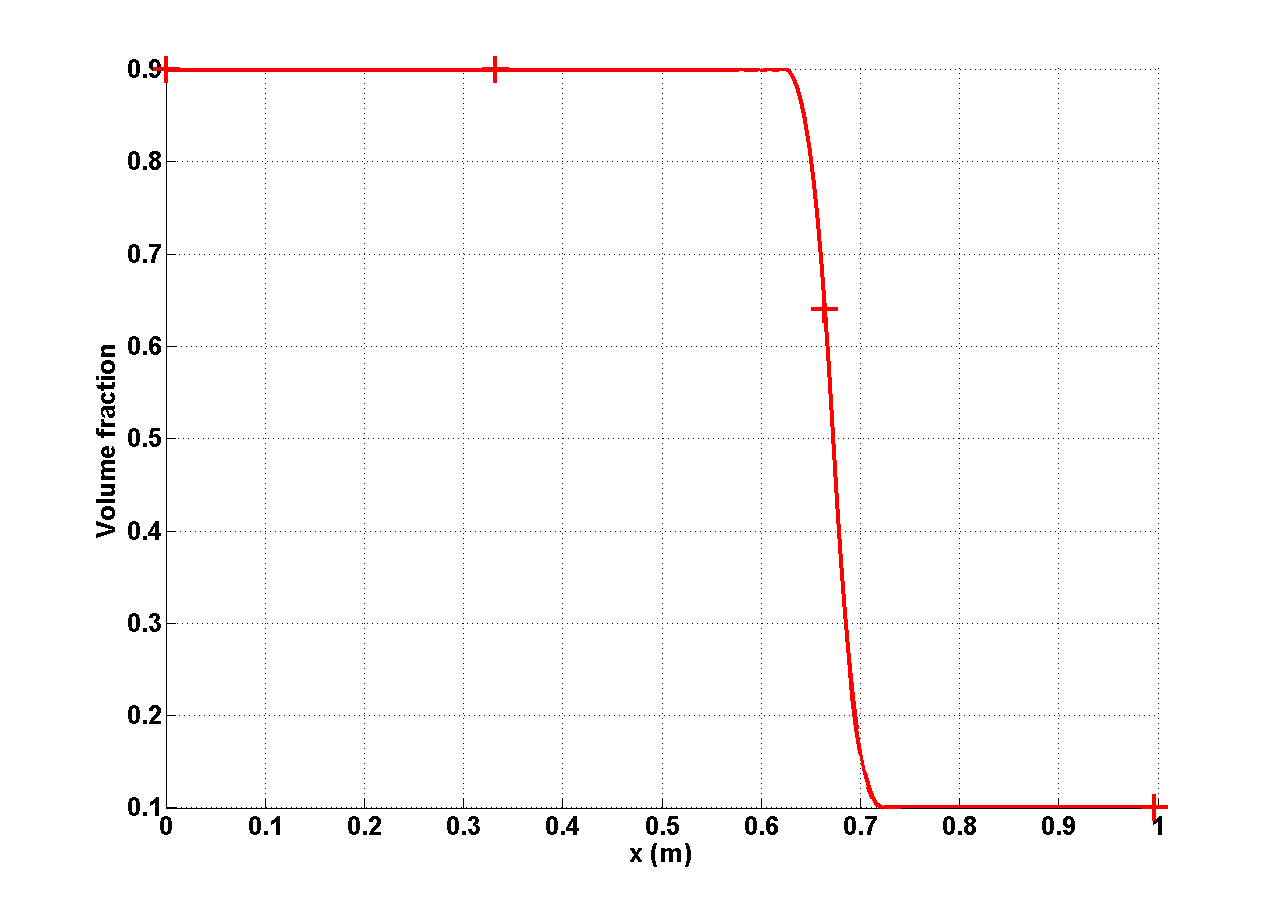
\includegraphics[width=\textwidth]{figures/SEM/liquid_volume_fraction.png}
                \caption{Volume fraction of phase 1.}
                \label{fig:vf-liq-7-eqn-sect4}
        \end{subfigure}%
        \begin{subfigure}[b]{0.495\textwidth}
                \centering
                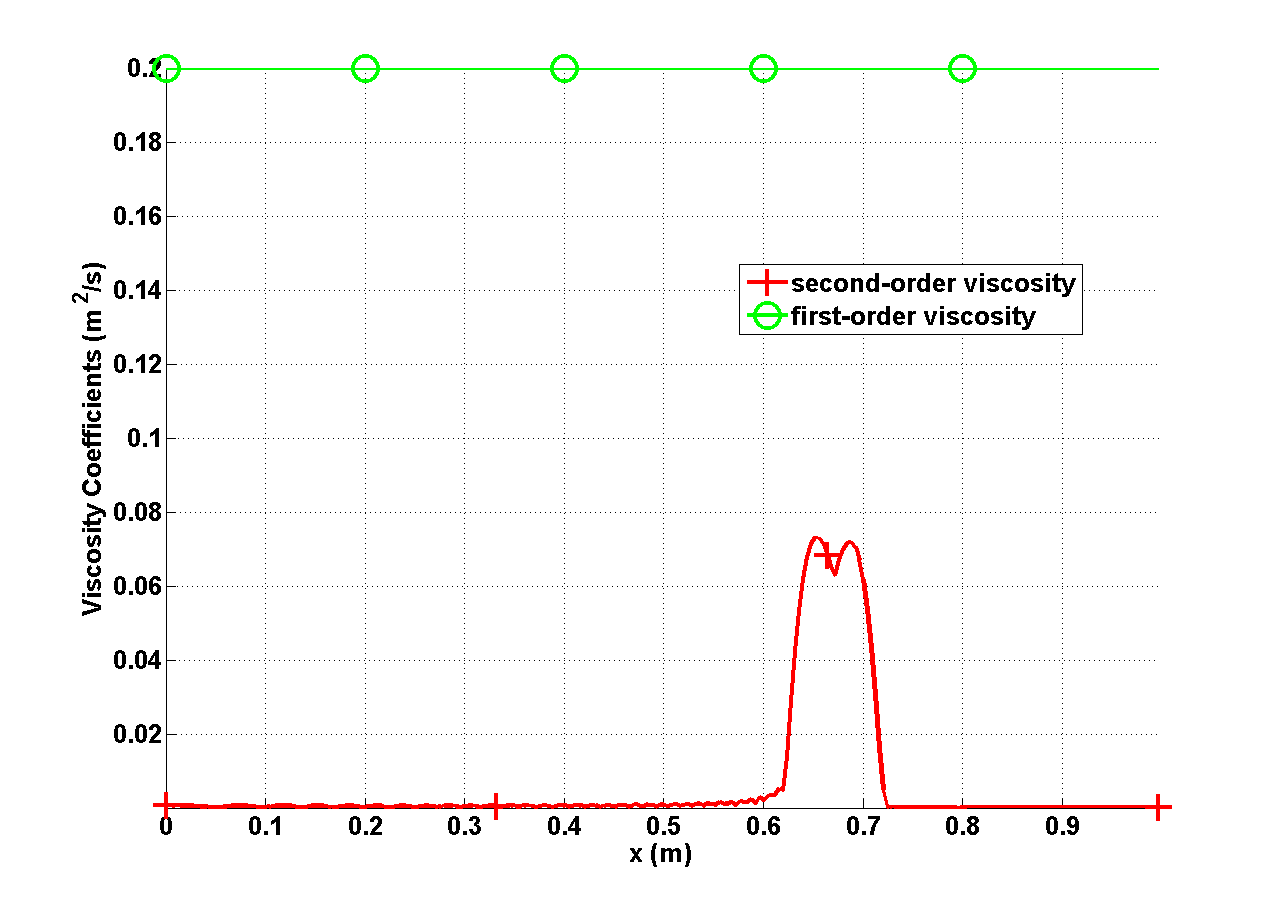
\includegraphics[width=\textwidth]{figures/SEM/liquid_beta.png}
                \caption{Viscosity coefficients for volume fraction equation of phase 1.}
                \label{fig:beta-liq-7-eqn-sect4}
        \end{subfigure}
        \caption{\label{fig:beta-visc-7-sect4}}
\end{figure}
%
\begin{figure}[H]
        \centering
        \begin{subfigure}[b]{0.495\textwidth}
                \centering
                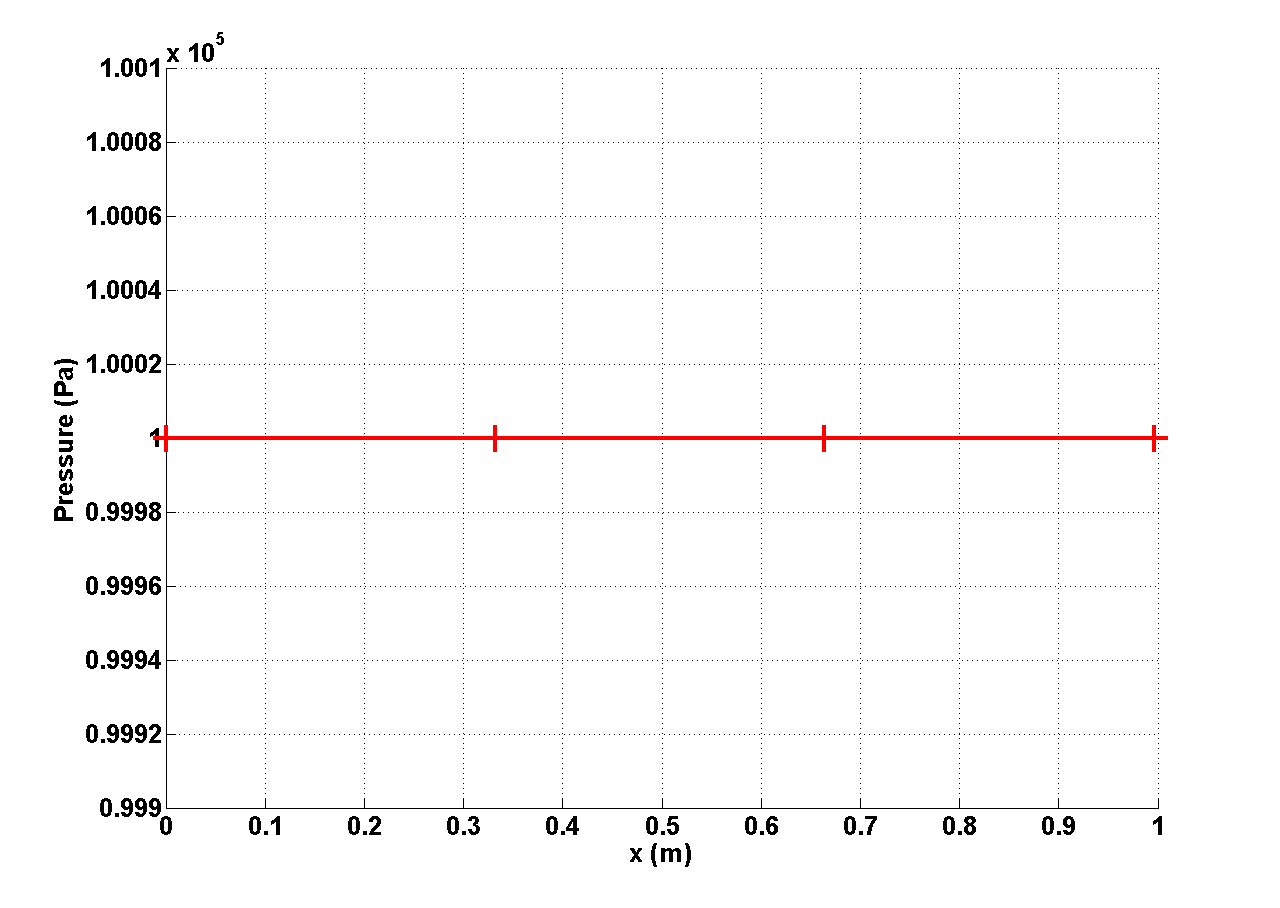
\includegraphics[width=\textwidth]{figures/SEM/liquid_pressure.png}
                \caption{Pressure of phase 1.}
                \label{fig:press-1-7-eqn-sect4}
        \end{subfigure}%
        \begin{subfigure}[b]{0.495\textwidth}
                \centering
                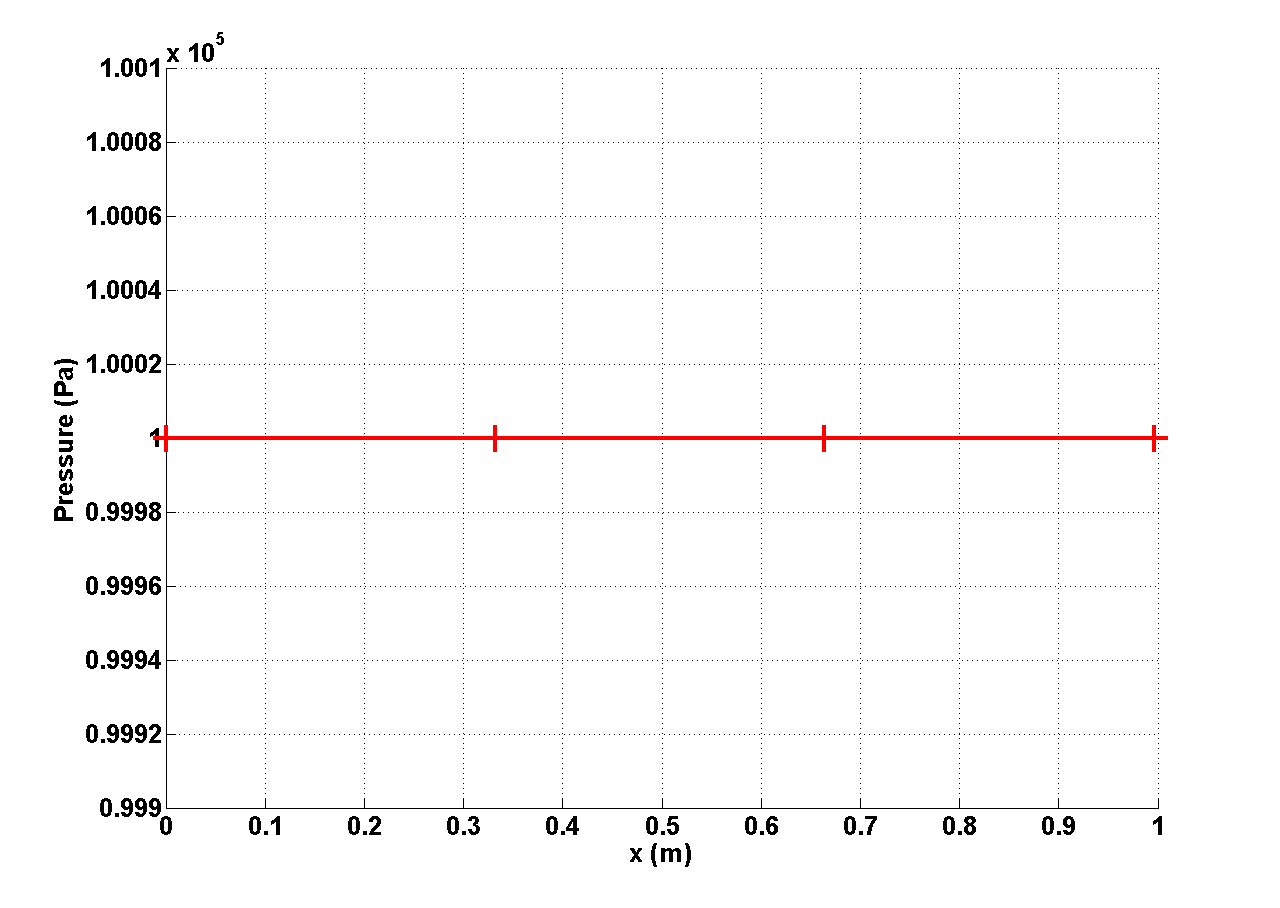
\includegraphics[width=\textwidth]{figures/SEM/vapor_pressure.png}
                \caption{Pressure of phase $2$.}
                \label{fig:press-2-7-eqn-sect4}
        \end{subfigure}
        \caption{\label{fig:press-7-sect4}}
\end{figure}
%
\begin{figure}[H]
        \centering
        \begin{subfigure}[b]{0.495\textwidth}
                \centering
                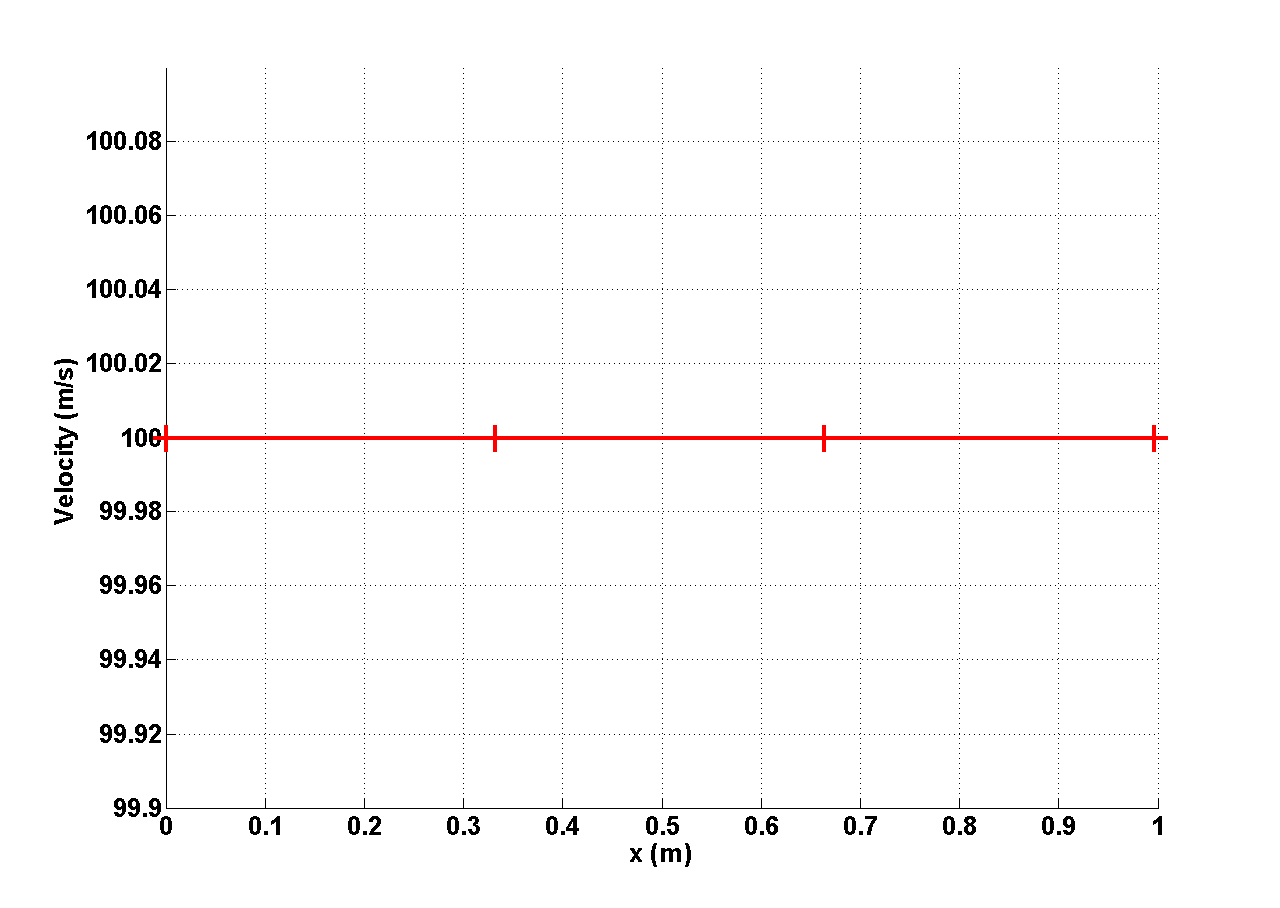
\includegraphics[width=\textwidth]{figures/SEM/liquid_velocity.png}
                \caption{Velocity of phase 1.}
                \label{ig:vel-1-7-eqn-sect4}
        \end{subfigure}%
        \begin{subfigure}[b]{0.495\textwidth}
                \centering
                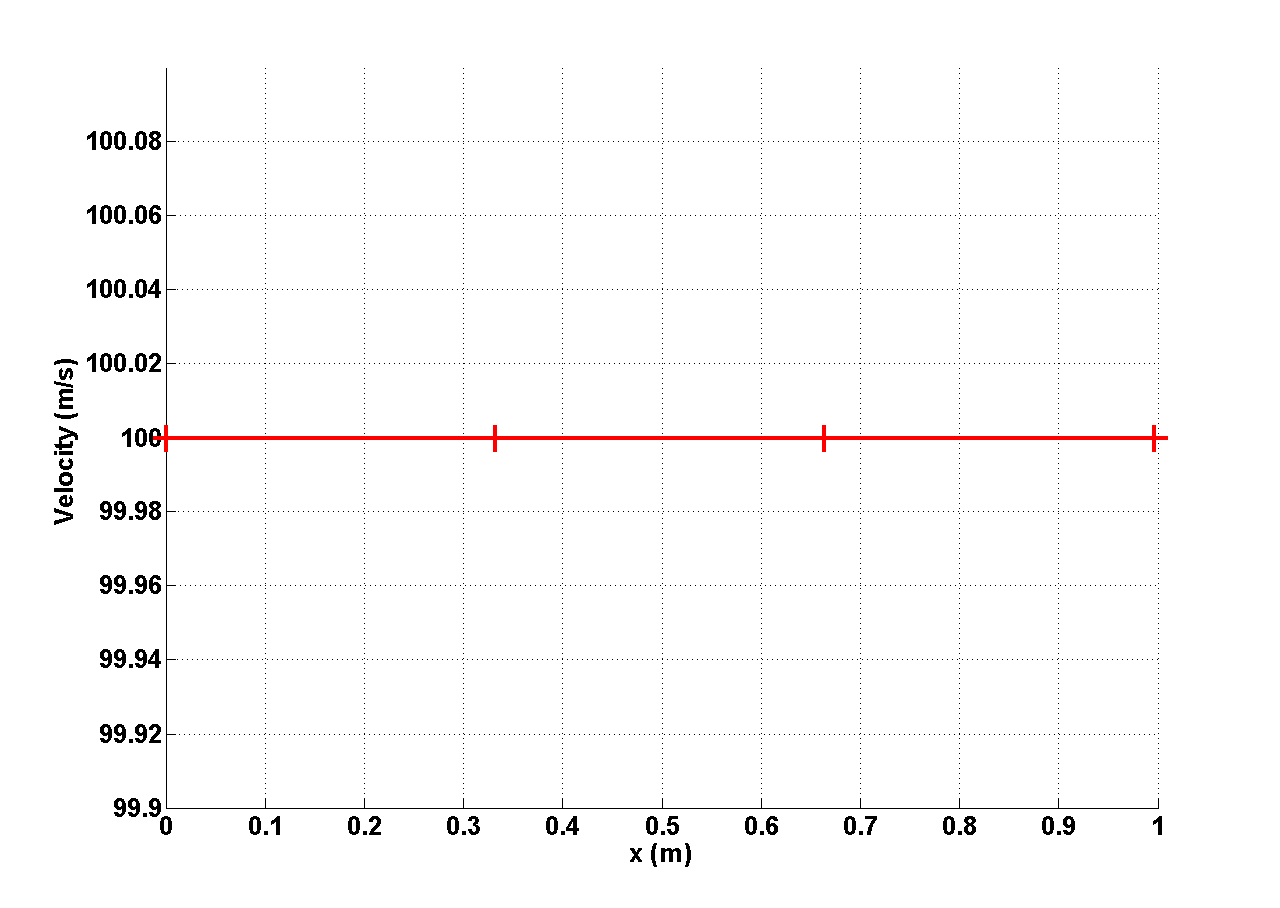
\includegraphics[width=\textwidth]{figures/SEM/vapor_velocity.png}
                \caption{Velocity of phase $2$.}
                \label{ig:vel-2-7-eqn-sect4}
        \end{subfigure}
        \caption{\label{fig:vel-7-sect4}}
\end{figure}
%
\begin{figure}[H]
        \centering
        \begin{subfigure}[b]{0.495\textwidth}
                \centering
                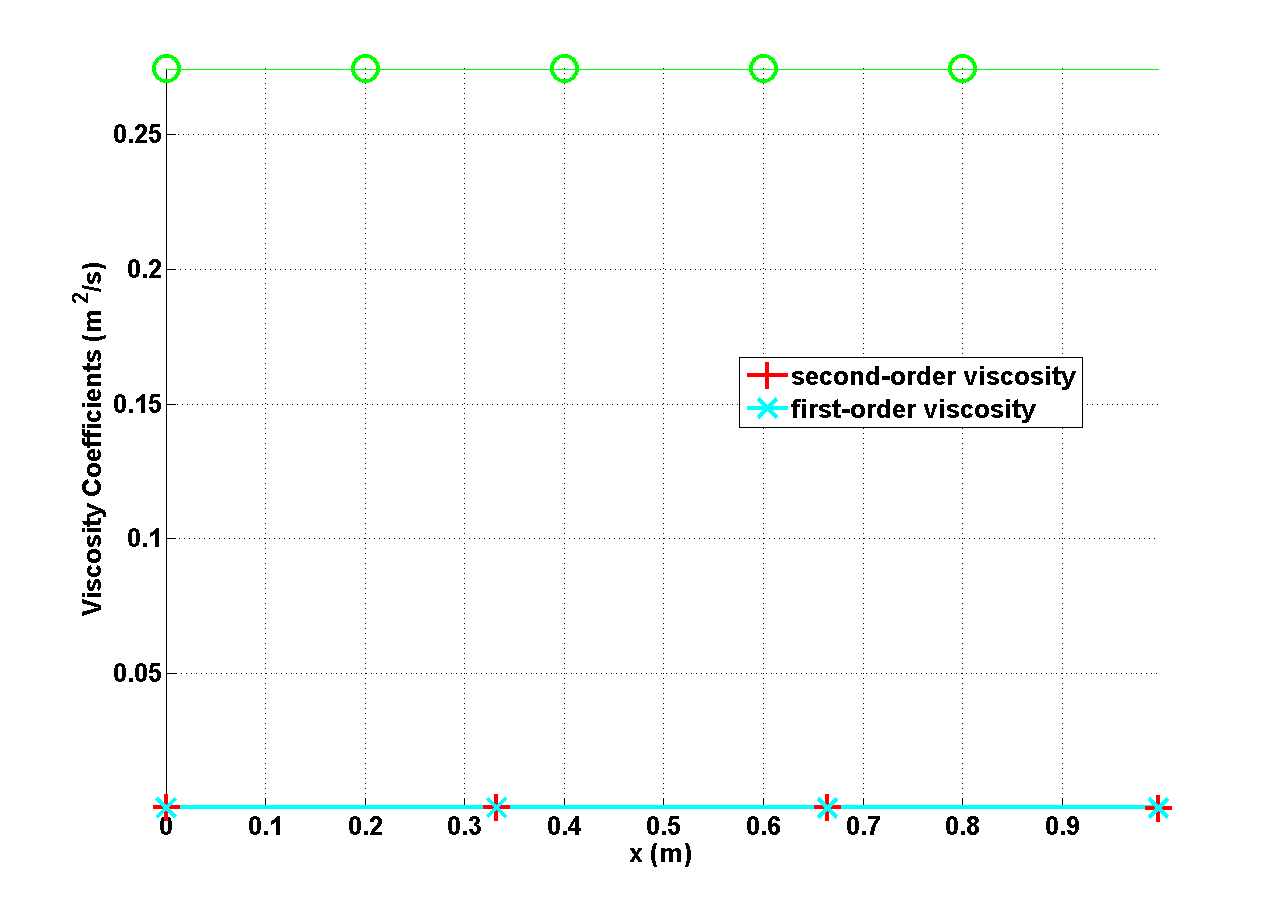
\includegraphics[width=\textwidth]{figures/SEM/liquid_viscosity.png}
                \caption{Viscosity coefficients of phase 1.}
                \label{ig:visc-1-7-eqn-sect4}
        \end{subfigure}%
        \begin{subfigure}[b]{0.495\textwidth}
                \centering
                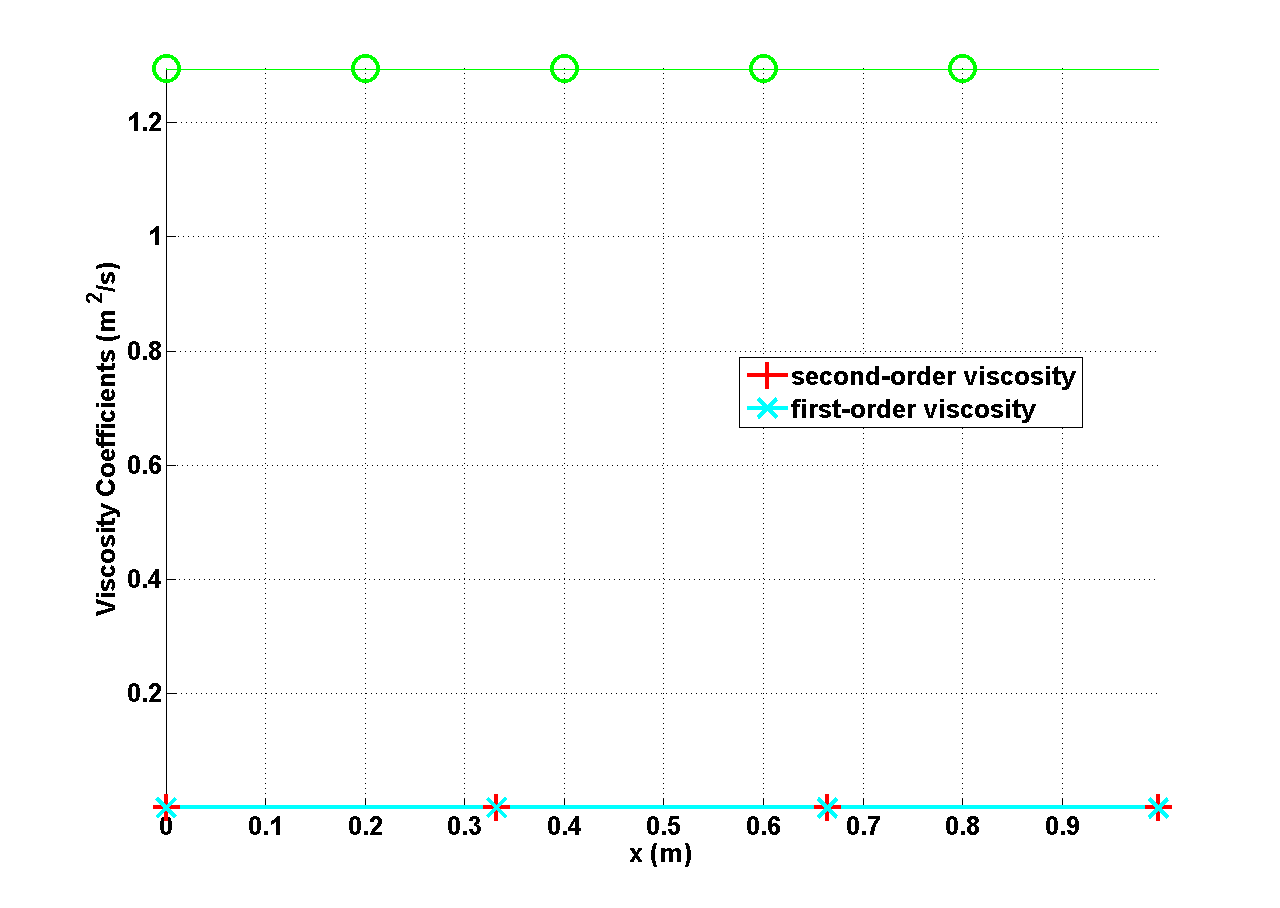
\includegraphics[width=\textwidth]{figures/SEM/vapor_viscosity.png}
                \caption{Viscosity coefficients of phase $2$.}
                \label{fig:visc-2-7-eqn-sect4}
        \end{subfigure}
        \caption{\label{fig:visc-7-sect4}}
\end{figure}
%
The stabilization numerical method preserves the uniform pressure (\fig{fig:press-7-sect4}) and velocity (\fig{fig:vel-7-sect4}) flow conditions while correctly resolving the discontinuity in the volume fraction profile as shown in \fig{fig:vf-liq-7-eqn-sect4}. The viscosity coefficients $\mu_k$ and $\kappa_k$ are equal to zero for both phases as shown in \fig{fig:visc-7-sect4}, since the flow conditions are uniform. However, the viscosity coefficient $\beta_k$ is peaked in the discontinuity region as expected. This test clearly shows that the stabilization method does not induce any artificial waves due to the smearing of the discontinuity in the volume fraction profile.
%-------------------------------------------------------------------------------------------------------------------------------------------------
\subsection{1-D shock tube for two independent fluids}\label{sec:1d-2-ind-phases-7-eq-sct4}
%-------------------------------------------------------------------------------------------------------------------------------------------------
We still consider a 1-D straight pipe of length $L=1$ $m$ filled with the same fluids as in \sect{sec:1d-advection-7-eq-sct4}. The diaphragm separates the pipe in two chambers with a high pressure ($P_{left} = 1$ $MPa$) on the left side and a low pressure ($P_{left} = 0.1$ $MPa$) in the right side. Both fluids are initially at rest. The volume fraction is set to $0.5$ which means each side of the chamber contains a mixture of two fluids with different equation of state parameters. Since the velocity and pressure relaxation coefficients $\mu_P$ and $\lambda_u$ are set to zero, the two fluids will behave independently to each other and the volume fraction is expected to remain uniform during the simulation. An exact solution is available for each fluid which simply corresponds to the single-phase exact solution. The geometry is discretized with an uniform mesh of 500 cells and run with a $CFL$ of one until $t_{final} = 305$ $\mu s$. The numerical and exact solutions are given from \fig{fig:two-indep-fluids-press-7-eqn-sect4} to \ref{fig:two-indep-fluids-vf-visc-1-7-eqn-sect4}.
%
\begin{figure}[H]
\centering
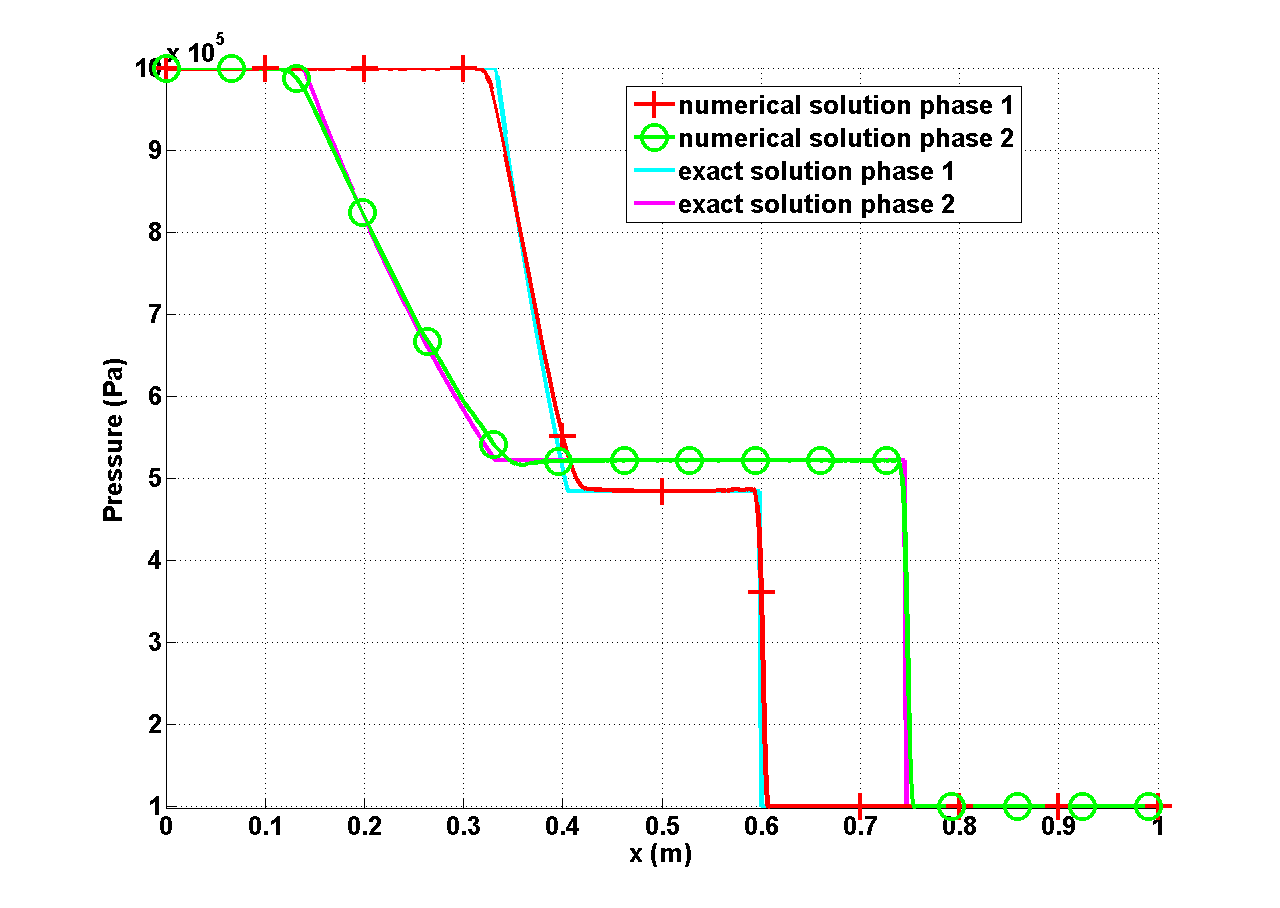
\includegraphics[width=\textwidth]{figures/SEM/two_phases_pressure.png}
\caption{Pressure profiles at $t=305$ $\mu s$.}
\label{fig:two-indep-fluids-press-7-eqn-sect4}
\end{figure}
%
\begin{figure}[H]
\centering
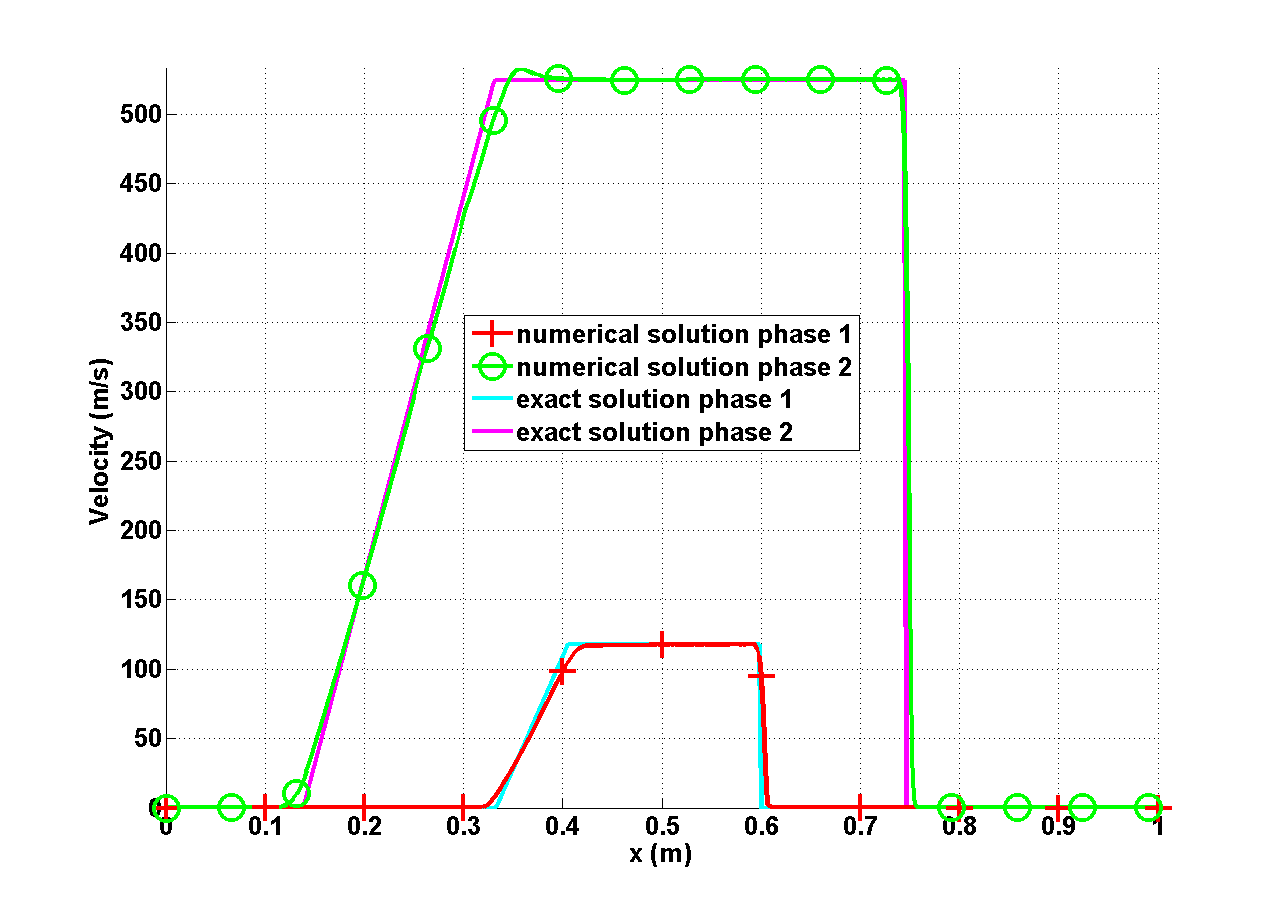
\includegraphics[width=\textwidth]{figures/SEM/two_phases_velocity.png}
\caption{Velocity profiles at $t=305$ $\mu s$.}
\label{fig:two-indep-fluids-vel-7-eqn-sect4}
\end{figure}
%
\begin{figure}[H]
\centering
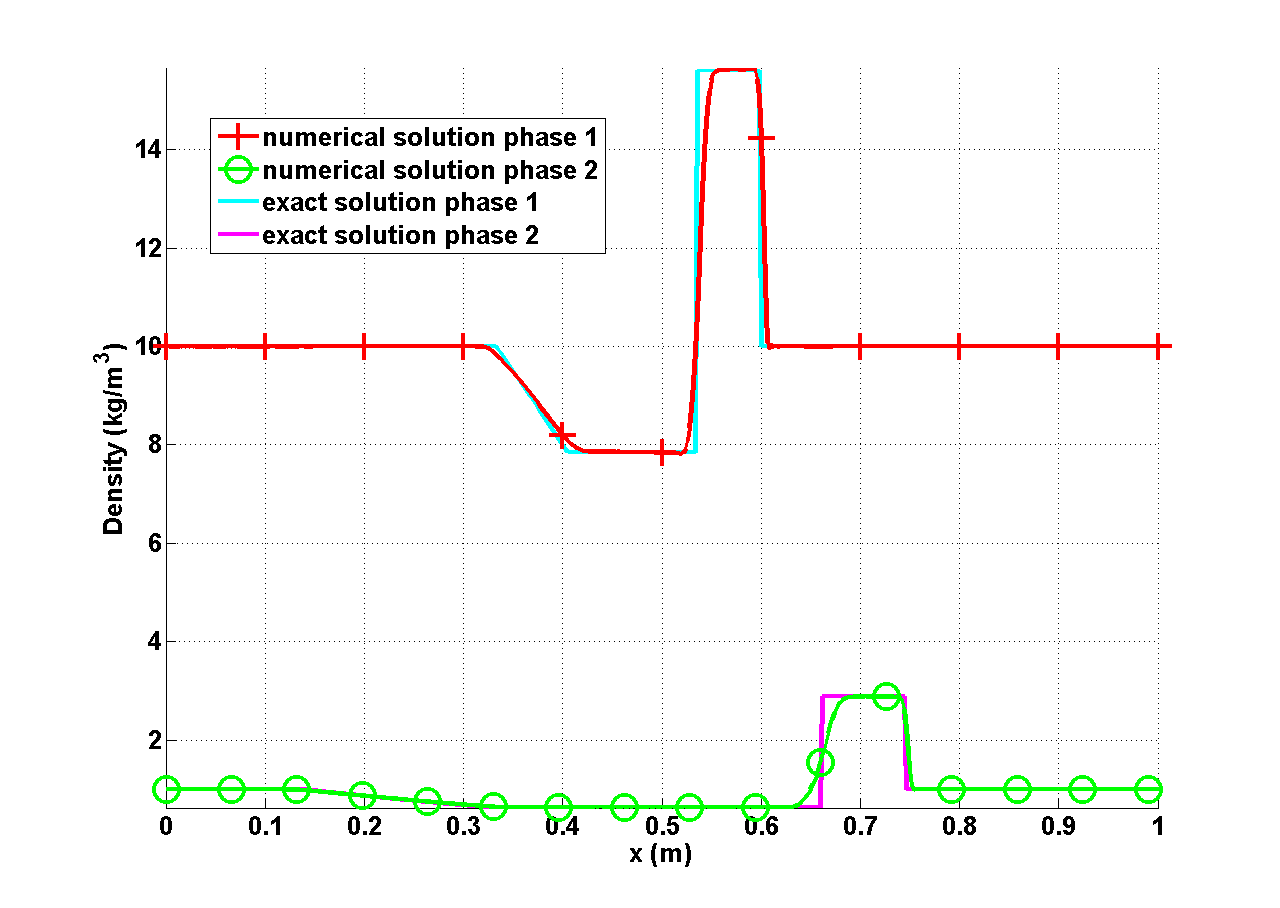
\includegraphics[width=\textwidth]{figures/SEM/two_phases_density.png}
\caption{Density profiles at $t=305$ $\mu s$.}
\label{fig:two-indep-fluids-dens-7-eqn-sect4}
\end{figure}
%
\begin{figure}[H]
\centering
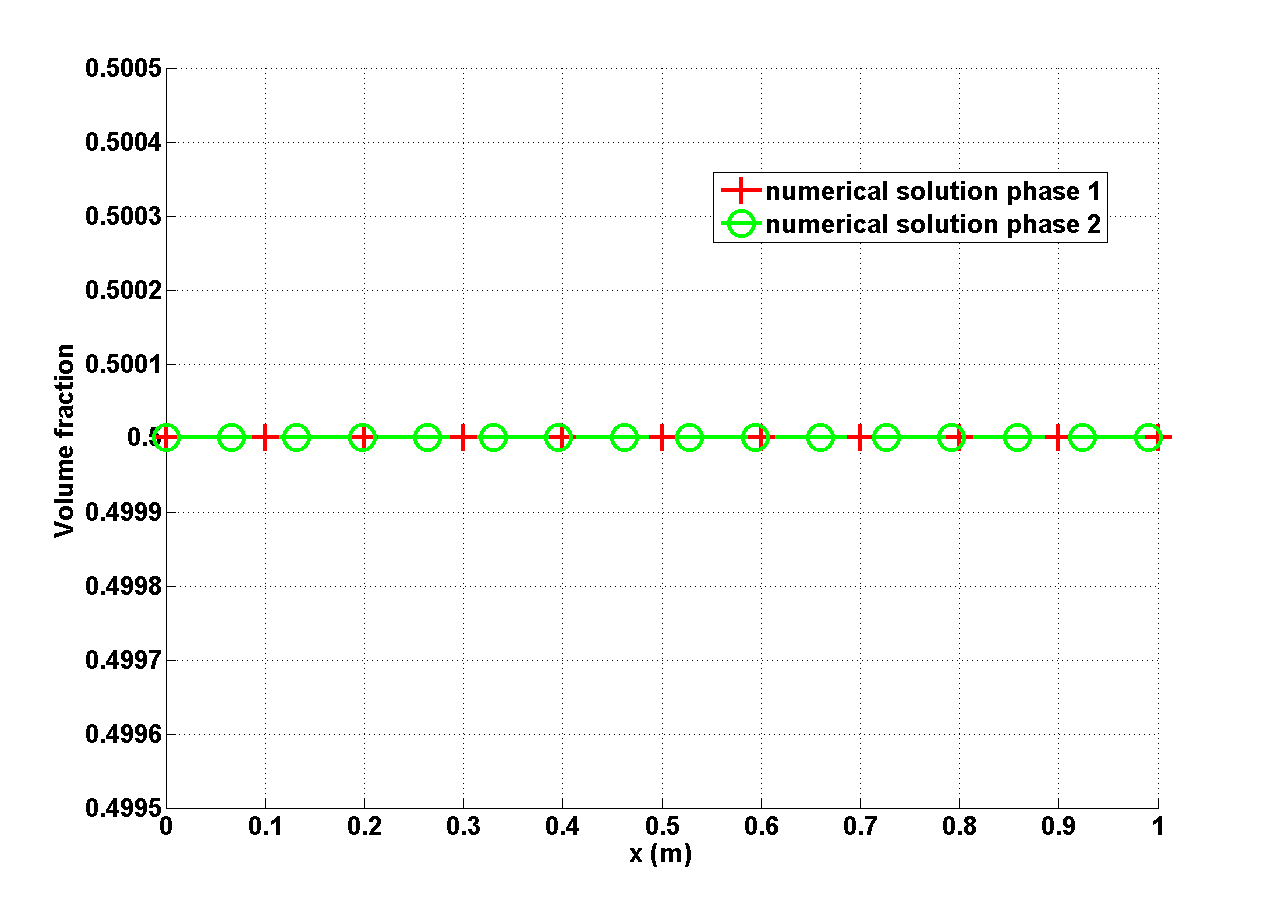
\includegraphics[width=\textwidth]{figures/SEM/two_phases_volume_fraction.png}
\caption{Volume fraction profiles at $t=305$ $\mu s$.}
\label{fig:two-indep-fluids-vf-7-eqn-sect4}
\end{figure}
%
\begin{figure}[H]
\centering
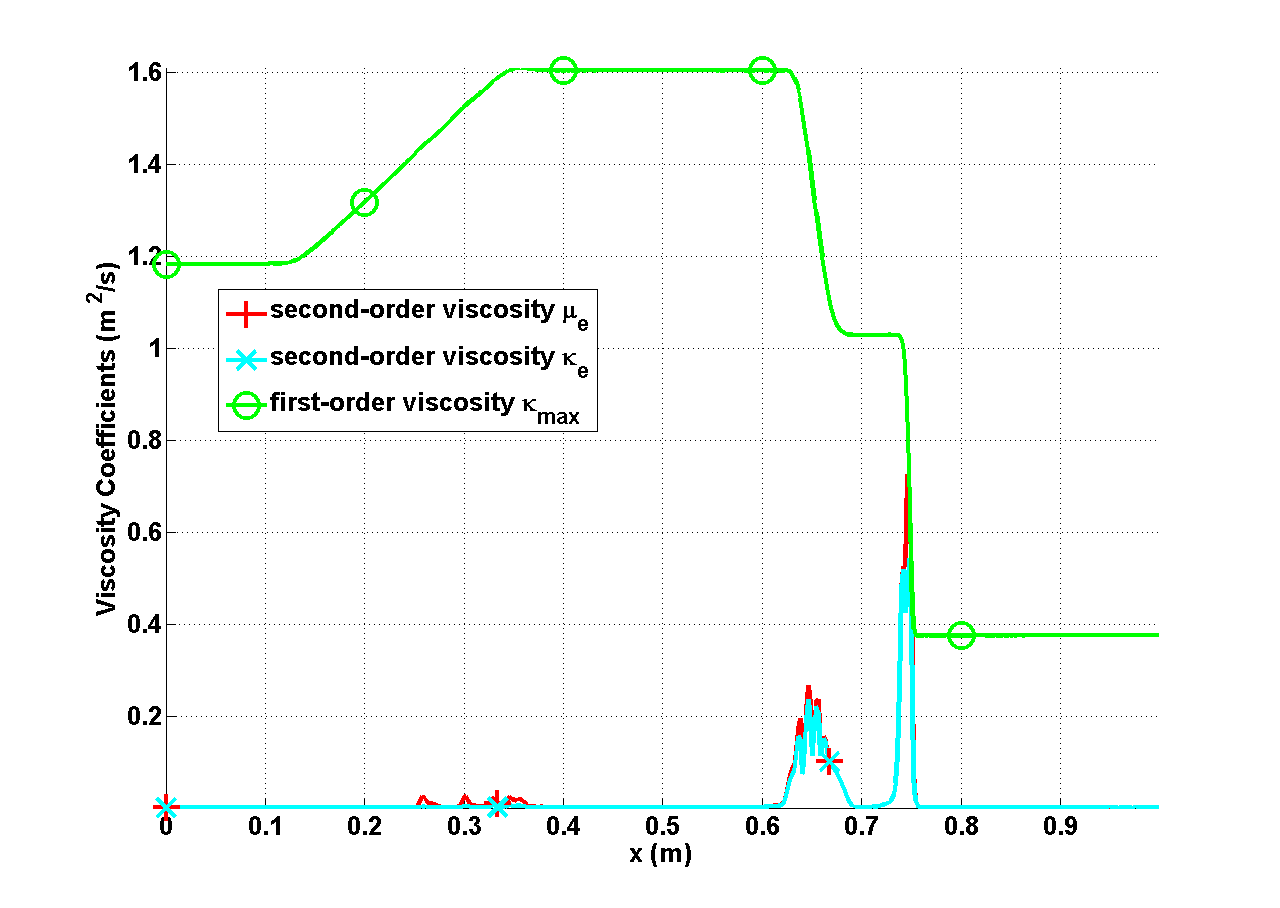
\includegraphics[width=\textwidth]{figures/SEM/two_phases_liquid_viscosity_kappa_mu.png}
\caption{Viscosity coefficient profiles for phase $2$ at $t=305$ $\mu s$.}
\label{fig:two-indep-fluids-visc-2-7-eqn-sect4}
\end{figure}
%
\begin{figure}[H]
\centering
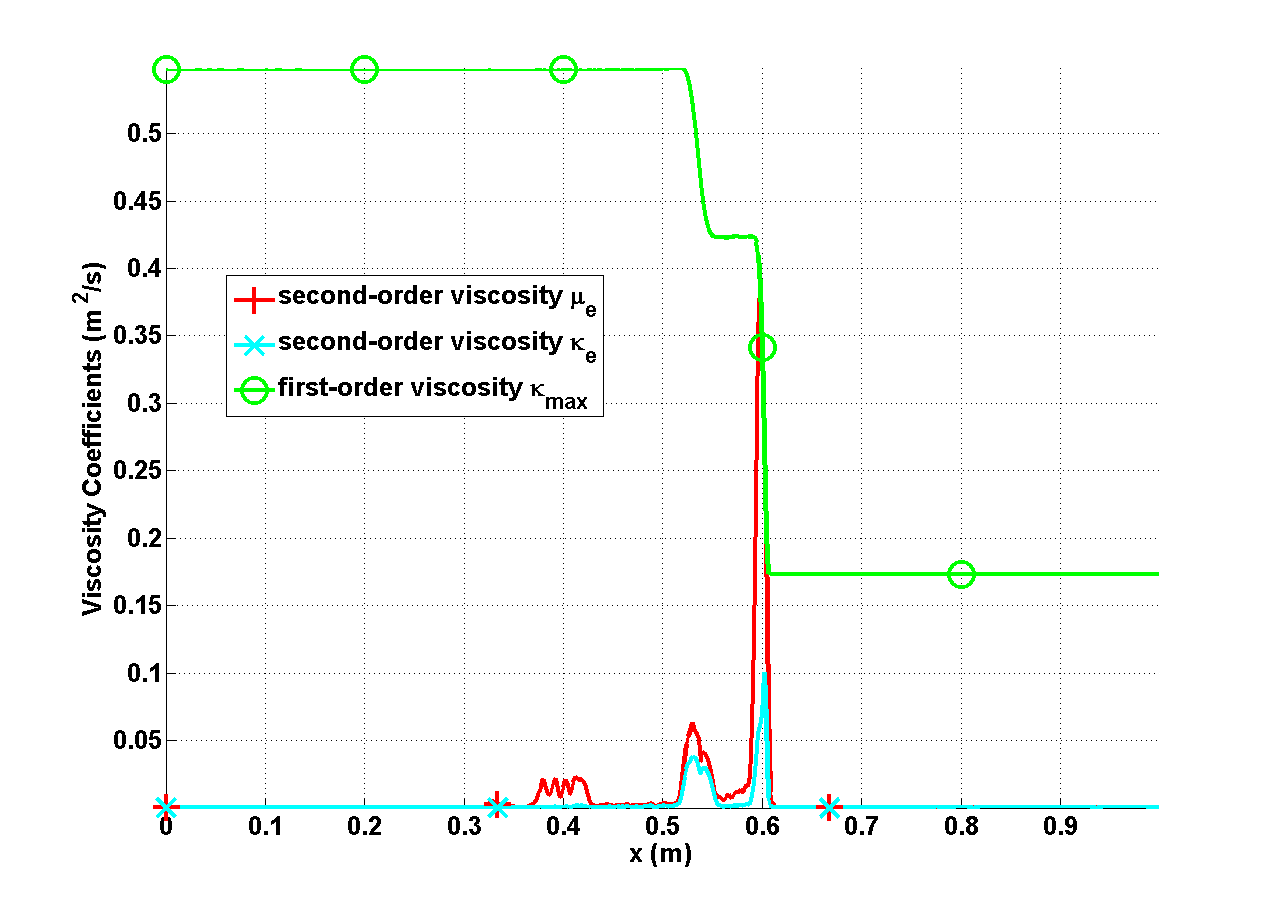
\includegraphics[width=\textwidth]{figures/SEM/two_phases_vapor_viscosity_kappa_mu.png}
\caption{Viscosity coefficient profiles for phase 1 at $t=305$ $\mu s$.}
\label{fig:two-indep-fluids-visc-1-7-eqn-sect4}
\end{figure}
%
\begin{figure}[H]
\centering
\includegraphics[width=\textwidth]{figures/SEM/two_phases_liquid_beta.png}
\caption{Viscosity coefficient profiles for volume fraction equation of phase 1 at $t=305$ $\mu s$.}
\label{fig:two-indep-fluids-vf-visc-1-7-eqn-sect4}
\end{figure}
%
The pressure, velocity and density profiles given in \fig{fig:two-indep-fluids-press-7-eqn-sect4}, \fig{fig:two-indep-fluids-vel-7-eqn-sect4} and \fig{fig:two-indep-fluids-dens-7-eqn-sect4}, respectively, show good agreement with the exact solutions for both phases. The fluid $2$ is lighter and thus experiences stronger variations: its velocity is larger and the shock moves faster. The viscosity coefficients shown in \fig{fig:two-indep-fluids-visc-2-7-eqn-sect4} and \fig{fig:two-indep-fluids-visc-1-7-eqn-sect4} for both phases have similar profiles: they are peaked in the shock regions and also display a bump in the contact wave. In \fig{fig:two-indep-fluids-vf-7-eqn-sect4}, it is noted that the volume fraction profiles remain uniform and are not altered by the variations in the other variables. The viscosity coefficient $\beta_k$ used in the volume fraction equation is zero (\fig{fig:two-indep-fluids-vf-visc-1-7-eqn-sect4}) as expected since the volume fraction profile is uniform.
%-------------------------------------------------------------------------------------------------------------------------------------------------
\subsection{1-D shock tube for two fluids with pressure and velocity relaxation terms}\label{sec:1d-2-phases-rel-7-eq-sct4}
%-------------------------------------------------------------------------------------------------------------------------------------------------
Once again, we consider a 1-D shock tube with the same initial conditions and the same fluids as in \sect{sec:1d-2-ind-phases-7-eq-sct4}. The pressure and velocity relaxation coefficients are no longer set to zero but computed from \eqt{E-R:85} and \eqt{E-R:86} with $A_{int,max} =  10^4$ $m^{-1}$\tcr{shouldn't it be Aintmax as used in eq 6.12? Just mention what you used for clarity } \tcb{done}. Thus, because of the relaxation source terms ($\mu_P \sim 4$ and $\lambda_u \sim 5 \times 10^5$ $s^{-1}$), the two fluids will exhibit the same pressure and velocity \tcr{give a ballpark value for relax params} \tcb{done}. The volume fraction will not remain uniform but is expected to vary due to the pressure relaxation source term (\eqt{eqn:multi-d-7-eqn-liq-vol}). For this test, an exact solution is not available but the reader can refer to \cite{Saurel_2007} for comparison. An uniform mesh of 500 cells is used. The code is run until $t_{final} = 305$ $\mu s$ with a CFL \tcr{italics in CFL. not consistent with the rest} \tcb{done} of one. The numerical solutions are presented from \fig{fig:two-fluids-rel-press-7-eqn-sect4} to \ref{fig:two-fluids-rel-vf-visc-1-7-eqn-sect4}.
%
\begin{figure}[H]
\centering
\includegraphics[width=\textwidth]{figures/SEM/relaxation_two_phases_pressure.png}
\caption{Pressure profiles at $t=305$ $\mu s$.}
\label{fig:two-fluids-rel-press-7-eqn-sect4}
\end{figure}
%
\begin{figure}[H]
\centering
\includegraphics[width=\textwidth]{figures/SEM/relaxation_two_phases_velocity.png}
\caption{Velocity profiles at $t=305$ $\mu s$.}
\label{fig:two-fluids-rel-vel-7-eqn-sect4}
\end{figure}
%
\begin{figure}[H]
\centering
\includegraphics[width=\textwidth]{figures/SEM/relaxation_two_phases_density.png}
\caption{Density profiles at $t=305$ $\mu s$.}
\label{fig:two-fluids-rel-rho-7-eqn-sect4}
\end{figure}
%
\begin{figure}[H]
\centering
\includegraphics[width=\textwidth]{figures/SEM/relaxation_two_phases_volume_fraction.png}
\caption{Volume fraction profiles at $t=305$ $\mu s$.}
\label{fig:two-fluids-rel-vf-7-eqn-sect4}
\end{figure}
%
\begin{figure}[H]
\centering
\includegraphics[width=\textwidth]{figures/SEM/relaxation_two_phases_liquid_viscosity_kappa_mu.png}
\caption{Viscosity coefficient profiles for phase 1 at $t=305$ $\mu s$.}
\label{fig:two-fluids-rel-visc-2-7-eqn-sect4}
\end{figure}
%
\begin{figure}[H]
\centering
\includegraphics[width=\textwidth]{figures/SEM/relaxation_two_phases_vapor_viscosity_kappa_mu.png}
\caption{Viscosity coefficient profiles for phase $2$ at $t=305$ $\mu s$.}
\label{fig:two-fluids-rel-visc-1-7-eqn-sect4}
\end{figure}
%
\begin{figure}[H]
\centering
\includegraphics[width=\textwidth]{figures/SEM/relaxation_two_phases_liquid_beta.png}
\caption{Viscosity coefficient profiles for volume fraction equation of phase 1 at $t=305$ $\mu s$.}
\label{fig:two-fluids-rel-vf-visc-1-7-eqn-sect4}
\end{figure}
%
As expected, the two fluids have the same pressure and velocity profiles as shown in \fig{fig:two-fluids-rel-press-7-eqn-sect4} and \fig{fig:two-fluids-rel-vel-7-eqn-sect4}, respectively. The shock is well resolved and does not display any instability. The main difference with the numerical results obtained in \sect{sec:1d-2-ind-phases-7-eq-sct4} lies in the volume fraction profiles that are no longer uniform but display a shock wave around $x=0.7$ $m$ as shown in \fig{fig:two-fluids-rel-vf-7-eqn-sect4}. Consequently, the viscosity coefficient $\beta_k$ is peaked in the shock region.  
%-------------------------------------------------------------------------------------------------------------------------------------------------
\subsection{1-D converging-diverging nozzle test}\label{sec:1d-nozzle-rel-7-eq-sct4}
%-------------------------------------------------------------------------------------------------------------------------------------------------
In this test, we propose to investigate the behavior of two fluids in a one-meter long 1-D converging-diverging nozzle with $A(x) = 1 + 0.5 \cos \left( 2\pi x \right)$. This test was first introduced by Saurel et al. in \cite{SEM} for the 1-D seven equation model and consists of a mixture of liquid water and vapor described by the SGEOS with the parameters given in \tbl{tbl:stff_gas_eos-sect4}.
%
\begin{table}[!htbp]
\begin{center}
\caption{ Stiffened Gas Equation of State parameters for steam and liquid water.}
\label{tbl:stff_gas_eos-sect4}
\begin{tabular}{|c|c|c|c|c|}
 \hline
\text{fluid}                           & $\gamma$ & $C_v$ $(J.kg^{-1}.K^{-1})$ & $P_\infty$ $(Pa)$ & $q$ $(J.kg^{-1})$ \\  \hline \hline
liquid water & 2.35     & 1816                       & $10^9$            & $-1167\ 10^3$     \\  \hline
steam          & 1.43     & 1040                       & 0                 & $ 2030\ 10^3$     \\  \hline
\end{tabular}
\end{center}
\end{table}
%
Stagnation boundary conditions are specified on the left of the nozzle (inlet) for both phases with a stagnation temperature $T_0 = 453 $ $K$ and a stagnation pressure $P_0 = 1$ $MPa$. At the outlet, a static pressure boundary condition is specified with $P = 0.5$ $MPa$ for both phases. The volume fraction is set to $\alpha_k = 0.5$ at the inlet. The initial conditions are computed from the boundary conditions by assuming the two fluids at rest and linearly interpolating the pressure and temperature between the boundary values. The geometry is discretized with an uniform mesh of 100 cells and run until steady-state. The pressure and velocity relaxation coefficients are computed from \eqt{E-R:85} and \eqt{E-R:86} and the use of \eqt{eq:Aint-sect4} for different values of $A_{int,max}$ that will be given later. The reader can refer to \sect {sec:liquid_nozzle} and \sect{sec:steam_nozzle} for numerical solutions in a 1-D nozzle when considering two independent fluids (i.e., without relaxation source terms). This section is organized as follows: first numerical results are presented when considering only the pressure and velocity relaxation terms for different values of $A_{int,max}$. Then, the same simulation is run when adding the mass and energy exchange source terms. \\

We first consider the 1-D seven equation model with on the relaxation source terms for different values of $A_{int,max} = 10^2 \text{, } 10^3$ and $10^4$ $m^{-1}$. The pressure profiles are given for all of the value of $A_{int,max}$ for comparison. The density, velocity, volume fraction and viscosity coefficients are only given for $A_{int,max} = 10^4$ $m^{-1}$. The numerical results are presented from \fig{fig:two-fluids-rel-nozzle-press-Aint4-sem-sect4} to \ref{fig:two-fluids-rel-nozzle-visc-vf-sem-sect4}.
%
\begin{figure}[H]
\centering
\includegraphics[width=\textwidth]{figures/SEM/Aint1e2_two_phases_pressure.png}
\caption{Pressure profiles at steady state with $A_{int,max} = 10^2$.}
\label{fig:two-fluids-rel-nozzle-press-Aint2-sem-sect4}
\end{figure}
%
\begin{figure}[H]
\centering
\includegraphics[width=\textwidth]{figures/SEM/Aint1e3_two_phases_pressure.png}
\caption{Pressure profiles at steady state with $A_{int,max} = 10^3$.}
\label{fig:two-fluids-rel-nozzle-press-Aint3-sem-sect4}
\end{figure}
%
\begin{figure}[H]
\centering
\includegraphics[width=\textwidth]{figures/SEM/Aint1e4_two_phases_pressure.png}
\caption{Pressure profiles at steady state with $A_{int,max} = 10^4$.}
\label{fig:two-fluids-rel-nozzle-press-Aint4-sem-sect4}
\end{figure}
%
The pressure profiles for $A_{int,max} = 10^2 \text{, } 10^3$ and $10^4$ $m^{-1}$ are given in \fig{fig:two-fluids-rel-nozzle-press-Aint2-sem-sect4}, \fig{fig:two-fluids-rel-nozzle-press-Aint3-sem-sect4} and \fig{fig:two-fluids-rel-nozzle-press-Aint4-sem-sect4} ,respectively. As the value of $A_{int,max}$ increases, the liquid pressure becomes positive and matches the vapor pressure variations. The static pressure outlet boundary holds for both phases. At the inlet, the liquid and vapor pressures are not equal since the implementation of the boundary condition does not account for the relaxation terms: the static pressure is computed from the stagnation pressure using entropy and enthalpy conservation relations. \tcr{add a small text, as we discussed with google chat} \tcb{done}
%
\begin{figure}[H]
\centering
\includegraphics[width=\textwidth]{figures/SEM/Aint1e4_two_phases_velocity.png}
\caption{Velocity profiles at steady state.}
\label{fig:two-fluids-rel-nozzle-vel-sem-sect4}
\end{figure}
%
\begin{figure}[H]
\centering
\includegraphics[width=\textwidth]{figures/SEM/Aint1e4_two_phases_density.png}
\caption{Density profiles at steady state.}
\label{fig:two-fluids-rel-nozzle-rho-sem-sect4}
\end{figure}
%
\begin{figure}[H]
\centering
\includegraphics[width=\textwidth]{figures/SEM/Aint1e4_two_phases_volume_fraction.png}
\caption{Volume fraction profiles at steady state.}
\label{fig:two-fluids-rel-nozzle-vf-sem-sect4}
\end{figure}
%
\begin{figure}[H]
\centering
\includegraphics[width=\textwidth]{figures/SEM/Aint1e4_liquid_viscosity_kappa_mu.png}
\caption{Viscosity coefficients profiles for liquid phase at steady state.}
\label{fig:two-fluids-rel-nozzle-visc-liq-sem-sect4}
\end{figure}
%
\begin{figure}[H]
\centering
\includegraphics[width=\textwidth]{figures/SEM/Aint1e4_vapor_viscosity_kappa_mu.png}
\caption{Viscosity coefficients profiles for vapor phase at steady state.}
\label{fig:two-fluids-rel-nozzle-visc-vap-sem-sect4}
\end{figure}
%
\begin{figure}[H]
\centering
\includegraphics[width=\textwidth]{figures/SEM/Aint1e4_liquid_beta.png}
\caption{Viscosity coefficients profiles for liquid volume fraction phase at steady state.}
\label{fig:two-fluids-rel-nozzle-visc-vf-sem-sect4}
\end{figure}
%
The velocity, density, volume fraction and viscosity coefficients profiles are plotted from \fig{fig:two-fluids-rel-nozzle-vel-sem-sect4} to \ref{fig:two-fluids-rel-nozzle-visc-vf-sem-sect4} in the case $A_{int,max} = 10^4$ $m^{-1}$. Because of the velocity relaxation source terms, velocity equilibrium holds between the liquid and vapor phases. The liquid and vapor density profiles are different by two order of magnitude. The volume fraction of both phases varies throughout the nozzle as a consequence of the pressure equilibrium. The viscosity coefficients $\mu_k$ and $\kappa_k$ are equal to each other since there are no shock waves and are large enough to stabilize the strong variations in the pressure and velocity profiles. Lastly, the viscosity coefficient $\beta_k$ follows the variations of the volume fraction for both phases. It is interesting to note that the fast vapor flow yields strong variations in the divergent part of the nozzle. Overall, the viscosity coefficients are large enough to prevent the formation of any numerical instability without altering the physical solution.\\
%

Next, the same converging-diverging nozzle is run with mass and energy exchange source terms. The code is run until steady-state with $A_{int,max}=10^3$ $m^{-1}$. The corresponding numerical results are shown from \fig{fig:two-fluids-rel-nozzle-press-mass-on-sem-sect4} to \ref{fig:two-fluids-rel-nozzle-visc-vf-mass-on-sem-sect4}.
%
\begin{figure}[H]
\centering
\includegraphics[width=\textwidth]{figures/SEM/Aint1e3MassOn_two_phases_pressure.png}
\caption{Pressure profiles at steady state with thermodynamic relaxations and mass and heat exchange terms.}
\label{fig:two-fluids-rel-nozzle-press-mass-on-sem-sect4}
\end{figure}
%
\begin{figure}[H]
\centering
\includegraphics[width=\textwidth]{figures/SEM/Aint1e3MassOn_two_phases_velocity.png}
\caption{Velocity profiles at steady state with thermodynamic relaxations and mass and heat exchange terms.}
\label{fig:two-fluids-rel-nozzle-vel-mass-on-sem-sect4}
\end{figure}
%
\begin{figure}[H]
\centering
\includegraphics[width=\textwidth]{figures/SEM/Aint1e3MassOn_two_phases_density.png}
\caption{Density profiles at steady state with thermodynamic relaxations and mass and heat exchange terms}
\label{fig:two-fluids-rel-nozzle-rho-mass-on-sem-sect4}
\end{figure}
%
\begin{figure}[H]
\centering
\includegraphics[width=\textwidth]{figures/SEM/Aint1e3MassOn_two_phases_volume_fraction.png}
\caption{Volume fraction profiles at steady state with thermodynamic relaxations and mass and heat exchange terms.}
\label{fig:two-fluids-rel-nozzle-vf-mass-on-sem-sect4}
\end{figure}
%
\begin{figure}[H]
\centering
\includegraphics[width=\textwidth]{figures/SEM/Aint1e3MassOn_liquid_viscosity_kappa_mu.png}
\caption{Viscosity coefficients profiles for liquid phase at steady state with thermodynamic relaxations and mass and heat exchange terms.}
\label{fig:two-fluids-rel-nozzle-visc-liq-mass-on-sem-sect4}
\end{figure}
%
\begin{figure}[H]
\centering
\includegraphics[width=\textwidth]{figures/SEM/Aint1e3MassOn_vapor_viscosity_kappa_mu.png}
\caption{Viscosity coefficients profiles for vapor phase at steady state with thermodynamic relaxations and mass and heat exchange terms.}
\label{fig:two-fluids-rel-nozzle-visc-vap-mass-on-sem-sect4}
\end{figure}
%
\begin{figure}[H]
\centering
\includegraphics[width=\textwidth]{figures/SEM/Aint1e3MassOn_liquid_beta.png}
\caption{Viscosity coefficients profiles for liquid volume fraction at steady state with thermodynamic relaxations and mass and heat exchange terms.}
\label{fig:two-fluids-rel-nozzle-visc-vf-mass-on-sem-sect4}
\end{figure}
%
Because of the mass and heat transfers between phases, the flow variations are smoother than in the previous case. Consequently, the viscosity coefficients are also smoother while effectively stabilizing the scheme.  
%-------------------------------------------------------------------------------------------------------------------------------------------------
\subsection{1-D straight pipe with wall-friction force, wall heat source and exchange terms (mass and energy)}\label{sec:1d-straight-pipe-7-eq-sct4}
%-------------------------------------------------------------------------------------------------------------------------------------------------
We present one sample result for a 1-D straight pipe of constant area $A = 10^{-4}$ $m^2$ with a wall heat source (the wall temperature is constant: $T_w = 550$ $K$). The stiffened gas equation of state is used to model the liquid and vapor phases with the parameters taken from \cite{SGEOS} for each phase. A static pressure of $P=7.1$ $MPa$ is set at the outlet. The volume fraction, the enthalpy and the mass flow rate are specified at the inlet for each phase. The wall friction coefficient is constant and the same for the two phases, $f_w = 4 \times 10^{-2}$. The interfacial area $A_{int}$ is set to a large value to equalize the pressure and velocity of the two phases. The initial conditions are uniform. The geometry is discretized with a uniform mesh of 100 elements and the simulation is run with CFL$=100$  until a steady state is obtained. 

The pressure, temperature, velocity, volume fraction and viscosity coefficients profiles are plotted from \fig{fig:pressure} through \fig{fig:viscosity_coeff}. As expected, the liquid and vapor pressure profiles are identical (\fig{fig:pressure}) and decrease throughout the domain because of wall friction. The liquid and velocity profiles are also identical as shown in \fig{fig:velocity} and increase due to the wall friction force and the heat addition. In \fig{fig:temperature}, the liquid and vapor temperature profiles are distinct and have the same variation: the temperature rises since energy is added to the flow by the wall heat source. The variations of the vapor and liquid volume fractions are opposite: vapor is produced since the liquid temperature is larger than the saturation temperature. All of the profiles are smooth and do not display any spurious oscillations: the entropy viscosity coefficients shown in \fig{fig:viscosity_coeff}, $\kappa_{e,k}$ and $\beta_{e,k}$, are well-scaled and large enough to stabilize the numerical solution without altering it (only $\beta_{e,liquid}$ is plotted since $\beta_{e,liquid}=\beta_{e,vapor}$). It is also noted the difference of several order of magnitude between the entropy viscosity and first-order viscosity coefficients denoted by the subscript $max$. The first-order viscosity coefficients are over-dissipative and ill-scaled in the low Mach regime.
%
        \begin{figure}[H]
                \centering
                \includegraphics[width=\textwidth]{figures/SEM/ANS_WINTER_2014_7Eqn_pressure.png}
                \caption{Pressure}
                \label{fig:pressure}
        \end{figure}%
%
        \begin{figure}[H]
                \centering
                \includegraphics[width=\textwidth]{figures/SEM/ANS_WINTER_2014_7Eqn_temperature.png}
                \caption{Temperature}
                \label{fig:temperature}
        \end{figure}%
%            
        \begin{figure}[H]
                \centering
                \includegraphics[width=\textwidth]{figures/SEM/ANS_WINTER_2014_7Eqn_velocity.png}
                \caption{Velocity}
                \label{fig:velocity}
        \end{figure}
%
        \begin{figure}[H]
                \centering
                \includegraphics[width=\textwidth]{figures/SEM/ANS_WINTER_2014_7Eqn_volume_fraction.png}
                \caption{Volume fraction}
                \label{fig:volume_fraction}
        \end{figure}        
%
        \begin{figure}[H]
                \centering
                \includegraphics[width=\textwidth]{figures/SEM/ANS_WINTER_2014_7Eqn_viscosity.png}
                \caption{Viscosity coefficients}
                \label{fig:viscosity_coeff}
        \end{figure}        
%
%Because it is not economical to solve the entire two-phase flow field
%with highly resolved three-dimensional computational fluid dynamics for an
%entire light water reactor coolant system,
%it is necessary to construct a one-dimensional model for flow in
%pipes, nozzles, and other components.  The one-dimensional model is
%constructed to allow the representation of continuously variable
%cross-sectional area.
%
%Consider flow through a duct with local cross-sectional area
%$A=A(x,t)$.  Actually, most of the time we consider local
%cross-sectional area to depend upon position coordinate $x$ only,
%for which a time rate of change of cross-sectional area is not
%necessary because for this case $\frac{\partial A}{\partial
%t} = 0$.  However, $A(x,t)$ is left inside the time derivative terms
%for generality and possible future use.  The seven-equation two-phase
%system model can be stated as balances of mass, momentum, and total energy,
%along with volume fraction evolution as
%\begin{align}
%  % liquid mass conservation
%  \label{E-R:74}
%  \frac{\partial \left( \alpha \rho \right)_{liq} A}{\partial t}
%  + \frac{\partial \left( \alpha \rho u \right)_{liq} A}{\partial x}
%  &= - \Gamma A_{int} A
%  \\
%  % liquid momentum
%  \nonumber
%  \frac{\partial \left( \alpha \rho u \right)_{liq} A}{\partial t}
%  + \frac{\partial \alpha_{liq} A \left( \rho u^2 + p \right)_{liq} }{\partial x}
%  &= p_{int} A \frac{\partial \alpha_{liq}}{\partial x} + p_{liq} \alpha_{liq} \frac{\partial A}{\partial x}
%  \\
%  \nonumber
%  &+ A \lambda_u (u_{vap} - u_{liq})
%  \\
%  \nonumber
%  &- \Gamma A_{int} u_{int} A
%  \\
%  \nonumber
%  &- F_{\text{wall friction}, liq} - F_{\text{friction}, vap}
%  \\
%  &+ \left( \alpha \rho \right)_{liq} A \vec{g} \cdot \vec{n}_{axis}
%\end{align}
%\begin{align}
%  % liquid total energy
%  \nonumber
%  \frac{\partial \left( \alpha \rho E \right)_{liq} A}{\partial t}
%  + \frac{\partial \alpha_{liq} u_{liq} A \left( \rho E + p \right)_{liq}}{\partial x}
%  &= p_{int} u_{int} A \frac{\partial \alpha_{liq}}{\partial x} - \bar{p}_{int} A \mu_P (p_{liq} - p_{vap})
%  \\
%  \nonumber
%  &+ \bar{u}_{int} A \lambda_u (u_{vap} - u_{liq})
%  \\
%  \nonumber
%  &+ \Gamma A_{int} \left( \frac{p_{int}}{\rho_{int}} - H_{liq, int} \right) A
%  \\
%  &+ Q_{int, liq} + Q_{\text{wall}, liq}
%  \\
%  % liquid volume fraction
%  \label{eqn:7eqn_va_alpha_liq}
%  \frac{\partial \alpha_{liq} A}{\partial t} + u_{int} A \frac{\partial \alpha_{liq}}{\partial x}
%  &= A \mu_P (p_{liq} - p_{vap}) - \frac{\Gamma A_{int} A}{\rho_{int}}
%\end{align}
%for the liquid phase, and
%\begin{align}
%  % vapor mass conservation
%  \frac{\partial \left( \alpha \rho \right)_{vap} A}{\partial t}
%  + \frac{\partial \left( \alpha \rho u \right)_{vap} A}{\partial x}
%  &=  \Gamma A_{int} A
%  \\
%  % vapor momentum
%  \nonumber
%  \frac{\partial \left( \alpha \rho u \right)_{vap} A}{\partial t}
%  + \frac{\partial \alpha_{vap} A \left( \rho u^2 + p \right)_{vap} }{\partial x}
%  &= p_{int} A \frac{\partial \alpha_{vap}}{\partial x} + p_{vap} \alpha_{vap} \frac{\partial A}{\partial x}
%  \\
%  \nonumber
%  &+ A \lambda_u (u_{liq} - u_{vap})
%  \\
%  \nonumber
%  &+ \Gamma A_{int} u_{int} A
%  \\
%  \nonumber
%  &- F_{\text{wall friction}, vap} - F_{\text{friction}, liq}
%  \\
%  &+ \left( \alpha \rho \right)_{vap} A \vec{g} \cdot \vec{n}_{axis}
%\end{align}
%\begin{align}
%  \nonumber
%  % vapor total energy
%  \frac{\partial \left( \alpha \rho E \right)_{vap} A}{\partial t}
%  + \frac{\partial \alpha_{vap} u_{vap} A \left( \rho E + p \right)_{vap}}{\partial x}
%  &= p_{int} u_{int} A \frac{\partial \alpha_{vap}}{\partial x} - \bar{p}_{int} A \mu_P (p_{vap} - p_{liq})
%  \\
%  \nonumber
%  &+ \bar{u}_{int} A \lambda_u (u_{liq} - u_{vap})
%  \\
%  \nonumber
%  &- \Gamma A_{int} \left( \frac{p_{int}}{\rho_{int}} - H_{vap, int} \right) A
%  \\
%  &+ Q_{int, vap} + Q_{\text{wall}, vap}
%  \\
%  % vapor phase volume fraction
%  \label{E-R:81}
%  \frac{\partial \alpha_{vap} A}{\partial t} + u_{int} A \frac{\partial \alpha_{vap}}{\partial x}
%  &= A \mu_P (p_{vap} - p_{liq}) + \frac{\Gamma A_{int} A}{\rho_{int}}
%\end{align}
%%%%%%%%%%%%%%%%%%%%%%%%%%%%%%%%%%%%%%%%%%%%%%%%%%%
%
%  New template code for TAMU Theses and Dissertations starting Fall 2012.  
%  For more info about this template or the 
%  TAMU LaTeX User's Group, see http://www.howdy.me/.
%
%  Author: Wendy Lynn Turner 
%	 Version 1.0 
%  Last updated 8/5/2012
%
%%%%%%%%%%%%%%%%%%%%%%%%%%%%%%%%%%%%%%%%%%%%%%%%%%%

%%%%%%%%%%%%%%%%%%%%%%%%%%%%%%%%%%%%%%%%%%%%%%%%%%%%%%%%%%%%%%%%%%%%%%%
%%%                           SECTION V
%%%%%%%%%%%%%%%%%%%%%%%%%%%%%%%%%%%%%%%%%%%%%%%%%%%%%%%%%%%%%%%%%%%%%%
\chapter{\uppercase {Application of the entropy viscosity method to the $1$-D grey radiation-hydrodynamic equations}}\label{chap:hydro}
%%%%%%%%%%%%%%%%%%%%%%%%%%%%%%%%%%%%%%%%%%%%%%%%%%%%%%%%%%%%%
%%%%%%%%%%%%%%%%%%%%%%%%%%%%%%%%%%%%%%%%%%%%%%%%%%%%%%%%%%%%%
\section{Backgrounds}\label{sec:back_sect5}
%%%%%%%%%%%%%%%%%%%%%%%%%%%%%%%%%%%%%%%%%%%%%%%%%%%%%%%%%%%%%
%%%%%%%%%%%%%%%%%%%%%%%%%%%%%%%%%%%%%%%%%%%%%%%%%%%%%%%%%%%%%
Solving the radiation hydrodynamic equations is a challenging task for multiple reasons. First, the characteristic time scales between the radiation and hydrodynamics are different by several orders of magnitude which often requires the radiation part to be solved implicitly to ensure stability. Second, as with any wave-dominated problems, high resolution schemes are needed to accurately resolve shocks. Third, achieving high-order accuracy is challenging but some recent developments provided high-order accuracy results both in time and space when discretizing either the Euler equations \cite{Hussaini, jlg1, jlg2, Leveque} or the radiation equation independently from each other. 

Significant effort has been put into developing Riemann solvers for both the radiation and hydrodynamic equations. Balsara \cite{Balsara} developed a Riemann solver for the radiation-hydrodynamic equations by considering the frozen approximation that decouples the two physics components. However, such an approach may be questionable in the equilibrium diffusion limit. In this case, the coupling terms drive the physics and have to be accounted for. A \emph{generalized Riemann solver} that accounts exactly for the relaxation terms was developed in \cite{Balsara}. Another approach assumes the strong equilibrium diffusion limit in which radiation diffusion is negligible and the radiation simply advects at the material velocity \cite{Woodward}. In this limit, the radiation hydrodynamics equation can be expressed in the form of the Euler equations with a radiation-modified equation of state (REOS) . Any solution technique for the Euler equations may be applied to these equations. Thus, one may develop approximate Riemann solvers for these equations and applied them in a general context. 

Edwards and al. \cite{EdwardsMorelLowrie} proposed a two-stage semi-implicit IMEX scheme to solve the coupled radiation-hydrodynamic equations. They applied a Trapezoidal/BDF2 temporal discretization scheme to the nonlinear grey radiation diffusion. The radiation and hydrodynamic equations are solved implicitly and explicitly, respectively. A Riemann solver along with a flux limiter is used to resolve shocks and other waves. Their results show good agreement with semi-analytical solutions. 

In this chapter we propose to solve the 1-D radiation-hydrodynamics equations by using \emph{the entropy viscosity method}. The methodology proposed in \sect{sec:hyp_sect1b} will be applied.
%This technique, developed by Guermond et al.  for hyperbolic systems of equations \cite{jlg1, jlg2}, consists in adding appropriate dissipative terms to the governing equations.  The viscosity coefficient of these terms is modulated by the local entropy production. These dissipative terms are devised to stabilize the numerical scheme and to remove the non-physical oscillations appearing at the shock locations. Generally speaking, entropy is produced at shocks \cite{Toro}. Thus, by setting the viscosity coefficient proportional to the entropy production, shocks can be detected and tracked and an adequate amount of viscosity is added locally to stabilize the numerical scheme. The entropy production is computed on the fly, by analyzing the entropy residual. This residual is strongly peaked in shocks and small elsewhere. 
%The entropy viscosity method was shown to achieve high-order accuracy away from the shock regions, was successfully applied to non-linear hyperbolic equations using various discretization methods (finite volume, continuous and discontinuous finite elements, spectral method) and yielded high-order accuracy on non-uniform meshes and complex geometries \cite{jlg2, valentin}. 
Because of the similarity between Euler equations and the radiation hydrodynamic equations, it is conjectured that the entropy viscosity method may be a good candidate for resolving shocks occurring in radiation-hydrodynamic phenomena.

The 1-D grey radiation-hydrodynamic (GRH) equations are recalled in \eqt{eq:equation1}:
\begin{equation}
\label{eq:equation1}
\left\{
\begin{array}{lll}
\partial_t \left( \rho \right) + \partial_x\left( \rho u \right) = 0 \\
\partial_t \left( \rho u\right) + \partial_x \left(\rho u^2 + P + \frac{\epsilon}{3} \right) = 0 \\
\partial_t \left( \rho E\right) + \partial_x \left[ u \left( \rho E + P \right) \right] = -\frac{u}{3} \partial_x \epsilon - \sigma_a c \left( a T^4 - \epsilon \right) \\
\partial_t \epsilon + \frac{4}{3} \partial_x \left( u \epsilon \right) = \frac{u}{3} \partial_x \epsilon + \partial_x \left( \frac{c}{3 \sigma_t} \partial_x \epsilon \right) + \sigma_a c \left( a T^4 - \epsilon \right)
\end{array}
\right. ,
\end{equation}
where $\rho$, $u$, $E$, $\epsilon$, $P$ and $T$ are the material density, material velocity, material specific total energy, radiation energy density, material pressure and temperature, respectively. The total and absorption cross sections, $\sigma_t$ and $\sigma_a$, are either constant or density- and temperature-dependent. The variables $a$ and $c$ are the Boltzman constant and the speed of light, respectively. Lastly, the symbols $\partial_t$ and $\partial_x$ denote the temporal and spatial partial derivatives, respectively. 
The material temperature and pressure are computed with the Ideal Gas equation of state (IGEOS):
\begin{equation}
\label{eq:equation2}
\left\{
\begin{array}{ll}
P = (\gamma-1) C_v \rho T \\
e = C_v T 
\end{array}
\right. ,
\end{equation}
where $e$ is the specific internal energy and is obtained from the expression $e = E - 0.5 u^2$. The heat capacity $C_v$ and the heat ratio coefficient $\gamma$ are assumed constant. 

The objective of this paper is to extend the entropy-based viscosity method to the 1-D grey radiation-hydrodynamic equations. The approach followed in this paper is similar to those of \cite{Balsara, LowrieMorel}: an infinite opacity is assumed and the relaxation terms are ignored in order to make \eqt{eq:equation1} hyperbolic. Then, an entropy equation is derived and used to obtain the functional forms of the viscous stabilization terms. Definitions for the viscosity coefficients are provided. 

This chapter is organized as follows. In \sect{sec:entropy-visc-meth_sct5}, the entropy viscosity method is extended to the grey radiation-hydrodynamic equations;  details regarding the derivation of the adequate dissipative terms and definitions for the new viscosity coefficients are provided. Numerical results are presented in \sect{sec:num-res} where the second-order accuracy of the scheme is demonstrated in both the equilibrium diffusion and streaming limits, using the method of manufactured solutions applied to the GRH equations. Then, several numerical test cases, taken from the published literature, are provided; in these simulations, the Mach number varies from $1.05$ to $50$ \cite{LowrieEdwards}.

%%%%%%%%%%%%%%%%%%%%%%%%%%%%%%%%%%%%%%%%%%%%%%%%%%%%%%%%%%%%%
%%%%%%%%%%%%%%%%%%%%%%%%%%%%%%%%%%%%%%%%%%%%%%%%%%%%%%%%%%%%%
\section{The entropy-based viscosity method applied to the 1-D Radiation-Hydrodynamic equations}\label{sec:entropy-visc-meth_sct5}
%%%%%%%%%%%%%%%%%%%%%%%%%%%%%%%%%%%%%%%%%%%%%%%%%%%%%%%%%%%%%
%%%%%%%%%%%%%%%%%%%%%%%%%%%%%%%%%%%%%%%%%%%%%%%%%%%%%%%%%%%%%

In this section, we extend the entropy viscosity method \cite{jlg1, jlg2, valentin} to the 1-D radiation-hydrodynamic equations in a staged process. First, the reader is guided through the main steps that lead to the derivation of the dissipative terms, using the entropy minimum principle \cite{entropy}. Then, a definition for the entropy viscosity coefficient based upon the entropy production is given. 

\noindent
We recall that the entropy viscosity method was developed for hyperbolic system of equations. However, the radiation hydrodynamic equations are not strictly hyperbolic but several numerical techniques are based on the study of their hyperbolic parts \cite{Balsara, LowrieMorel}. Thus, following the same rationale, the system of equations given in \eqt{eq:equation1} is made hyperbolic by assuming an infinite opacity (the frozen approximation) and by ignoring the relaxation terms. These two assumptions yield the following system of equations:
\begin{equation}
\label{eq:equation3}
\left\{
\begin{array}{lll}
\partial_t \left( \rho \right) + \partial_x\left( \rho u \right) = 0 \\
\partial_t \left( \rho u\right) + \partial_x \left(\rho u^2 + P + \frac{\epsilon}{3} \right) = 0 \\
\partial_t \left( \rho E\right) + \partial_x \left[ u \left( \rho E + P \right) \right] = -\frac{u}{3} \partial_x \epsilon\\
\partial_t \epsilon + \frac{4}{3} \partial_x \left( u \epsilon \right) = \frac{u}{3} \partial_x \epsilon
\end{array}
\right. .
\end{equation}
The jacobian matrix of the hyperbolic terms can be computed to derive the eigenvalues:
\begin{equation}
\label{eq:equation4}
\lambda_1 = u-c_m \text{, } \lambda_{2,3} = u \text{ and } \lambda_4 = u+c_m ,
\end{equation}
where $c_m$ is the radiation-modified material speed of sound and is defined as follows:
\begin{equation}
\label{eq:equation5}
c_m^2 = \underbrace{P_{\rho} + \frac{P}{\rho^2}P_e}_{c_{Euler}^2} + \frac{4 \epsilon}{9\rho}
\end{equation}
with $P_x$ the standard shorthand notation for $\partial_x P$, and $c^2_{Euler}$ denotes the definition of the speed of sound when considering only the 1-D Euler equations.
The above hyperbolic system of equations can be recast in a conservative form. This allows us to assume the existence of an entropy function $s$ \cite{Lax} that depends upon the internal energy $e$, the density $\rho$, and the radiation energy density $\epsilon$. Following some algebra given in \app{app:appendixA}, an equation satisfied by the entropy $s$ is obtained:
\begin{equation}
\label{eq:equation6}
\rho \frac{Ds}{Dt} = \rho \left( \partial_t s + u \partial_x s \right) = 0 \text{, }
\end{equation}
where $\frac{D \cdot}{Dt}$ denotes the total or material derivative. \eqt{eq:equation6} is referred to as the entropy residual and is used to prove the entropy minimum principle, $\frac{Ds}{Dt} \geq 0$, \cite{entropy}.

When adding dissipative terms to each equation of \eqt{eq:equation3} as required in the entropy viscosity method, the entropy residual equation is modified and some additional terms will appear in the right-hand side of \eqt{eq:equation6}. The sign of these extra terms needs to be studied for the entropy minimum principle to hold. As such, the entropy minimum principle is invoked to guide in the derivation of appropriate expressions for each of the dissipative terms. Obtaining the final expression of the dissipative terms is a lengthy process and only the final result along with the key assumptions are stated here. The reader is referred to \app{app:appendixA} for the details of the derivation. The system of equations with the dissipative terms is as follows:
\begin{equation}
\label{eq:equation7}
\left\{
\begin{array}{lll}
\partial_t \left( \rho \right) + \partial_x\left( \rho u \right) = \partial_x \left( \kappa \partial_x \rho \right) \\
\partial_t \left( \rho u\right) + \partial_x \left(\rho u^2 + P + \frac{\epsilon}{3} \right) = \partial_x \left( \kappa \partial_x \rho u \right) \\
\partial_t \left( \rho E\right) + \partial_x \left[ u \left( \rho E + P \right) \right] + \frac{u}{3} \partial_x \epsilon = \partial_x \left( \kappa \partial_x(\rho E) \right)\\
\partial_t \epsilon + \frac{4}{3} \partial_x \left( u \epsilon \right) - \frac{u}{3} \partial_x \epsilon = \partial_x \left( \kappa \partial_x \epsilon \right)
\end{array}
\right. ,
\end{equation}
where $\kappa$ is a locally defined positive viscosity coefficient. It was assumed the following conditions hold:
\begin{equation}
\label{eq:equation7bis}
\left\{
\begin{array}{ll}
P \frac{\partial s}{\partial e} + \rho^2 \frac{\partial s}{\partial \rho} + \frac{4}{3} \rho \epsilon \frac{\partial s}{\partial \epsilon} = 0 \\
s( \rho, e, \epsilon) = \hat{s}(\rho, e) + \frac{\rho_0}{\rho}\tilde{s}(\epsilon) 
\end{array}
\right.
\end{equation}
where $\tilde{s}$ is concave with respect to the radiation energy density $\epsilon$ and $\hat{s}$ is concave with respect to the internal energy $e$ and the specific volume $\rho^{-1}$. The constant $\rho_0$ is of order one and appears only for dimensionality purposes. The function $\hat{s}$ and $\tilde{s}$ are both physical entropy functions.\\
Once the dissipative terms are obtained, it remains to define the local viscosity coefficient $\kappa(x,t)$. Note that at the difference of the multi-D Euler equations of \sect{chap:euler}, only one viscosity coefficient is required since the low Mach asymptotic limit is not investigated in this chapter. In other word, it is assumed that $\mu(x,t) = \kappa(x,t)$ following the notations used in \sect{chap:euler}. 
We require the following to hold in the prescription for $\kappa$:
\begin{itemize}
\item Since the entropy residual is a measure of the entropy production that occurs in shock regions, it is natural to define a viscosity coefficient proportional to the entropy residual. This will enable shock detection and tracking and will also provide a measure of the viscosity required to stabilize the scheme. This viscosity coefficient is referred to as the \emph{entropy viscosity coefficient} or \emph{second-order viscosity coefficient} and is denoted by $\kappa_e(x,t)$.
\item An upper bound on $\kappa$ is to be set since entropy production can be very large in shocks. For explicit time integration, the maximum value of the viscosity coefficient is related to the Courant-Friedrichs-Lewy number (CFL). The upper bound on  $\kappa$  is defined by analogy to the standard upwind (Godunov) scheme that is known to efficiently smooth out oscillations (but is only first-order accurate). With implicit temporal integrators, the same reasoning is used even if the CFL number may not need to be strictly respected. This upper bound will be referred to as the \emph{first-order viscosity}, denoted by $\kappa_{max}(x,t)$.  
\item The viscosity coefficient $\kappa$ that is actually used in the dissipative terms of \eqt{eq:equation3} is defined as follows: $\kappa(x,t) = \min ( \kappa_e(x,t), \kappa_{max}(x,t) )$. With such a definition, the viscosity added to the system of equations will saturate to the first order viscosity in the shock regions. Elsewhere, the entropy production and thus the viscosity coefficient $\kappa$ are expected to be small.
\end{itemize}

Next, we define the local first- and second-order viscosity coefficients $\kappa_{max}(x,t)$ and $\kappa_e(x,t)$, respectively. Following the work of Zingan et al. \cite{valentin}, the first-order viscosity definition is based on the local largest eigenvalue that is known to be $|u| + c_m$ in 1-D:
\begin{equation}
\label{eq:equation8}
\kappa_{max} = \frac{h}{2} \left( |u| + c_m \right)
\end{equation}  
where $h$ is the local grid size. This definition is derived based on the upwind scheme and a simple derivation can be found in \cite{jlg1} in the case of a scalar hyperbolic equation. Through the definition of the radiation-modified speed of sound $c_m$, both the material and radiation properties are accounted for in the definition of the first-order viscosity coefficient.

\noindent 
The definition of the second order viscosity coefficient $\kappa_e(x,t)$ is based upon the entropy residual (\eqt{eq:equation6}) recast as a function of pressure $P$, density $\rho$ and radiation energy density $\epsilon$:
\begin{equation}
\label{eq:equation9}
R(x,t) = \frac{s_e}{P_e} \underbrace{ \left( \frac{dP}{dt} - c_{Euler}^2 \frac{d\rho}{dt} \right)}_\textrm{$\hat{R}(x,t)$}
\end{equation}
The term $s_e$ is the inverse of the material temperature (\app{app:appendixA}) and $P_e$ is computed from the IGEOS. These two terms are positive so that the sign of the entropy residual $R(x,t)$ can be determined by simply inspecting the terms inside the parentheses, denoted by $\hat{R}(x,t)$. Such an expression is easier to compute than the one given in \eqt{eq:equation6} which required an analytical expression for the entropy function. In addition to the entropy residual, inter-element jumps in the pressure and density gradients, $J$, are also accounted for. The objective is to be able to also detect discontinuities that are not shocks, such as contact waves (there is no entropy production in a contact wave), in order to stabilize them as well. \\
Thus, the entropy viscosity coefficient $\kappa_e(x,t)$ is set to be proportional to $\hat{R}(x,t)$ and $J$ with the following form: 
\begin{equation}
\label{eq:equation12}
\kappa_e(x,t) = h^2 \frac{\max (|\hat{R}(x,t)|, J)}{n_P}
\end{equation} 
where $J = \max_i (J(x_i,t))$, and $J(x_i,t)$ is the jump of a given quantity at cell interface $x_i$, and $n_P$ is a normalization function (of the same units as pressure) that has to be chosen so that the viscosity coefficient $\kappa$ has units of $m^2/s$. The following definition for the normalization function has been chosen: $n_P = \rho c_m^2$. Thus, the final definition for the viscosity coefficient $\kappa$ is the following:
\begin{equation}
\label{eq:equation12bis}
\kappa_e(x,t) = h^2 \frac{\max (|\hat{R}(x,t)|, J)}{\rho c_m^2}
\end{equation} 
The jump $J$ in the definition of $\kappa(x,t)$ is piecewise-constant. Its definition is discretization-dependent and defined as follows for Continuous Galerkin FEM: 
\begin{equation}
\label{eq:equation12ter}
\left\{
\begin{array}{lll}
J_P(x_i,t) = |u| [[\partial_x P]]\\
J_{\rho}(x_i,t) = c_m^2 |u|  [[\partial_x \rho]] \\
J(x_i,t) = \max( J_{\rho}(x_i,t), J_{P}(x_i,t) )
\end{array}
\right.
\end{equation}
The symbol $[[ \cdot ]]$ denotes the jump at the cell interface.

The entropy viscosity method is now well defined for the hyperbolic system given in \eqt{eq:equation3} and will be used to solve for the grey radiation-hydrodynamic equations given in \eqt{eq:equation1}. However, one may question how the relaxation source terms, $\sigma_a c (a T^4-\epsilon)$ and the physical diffusion term, $\partial_x(D\partial_x \epsilon)$, may affect the entropy viscosity method. When applying the entropy viscosity method, the radiation energy density equation will now contain a diffusive term and a numerical dissipative term with a vanishing viscosity coefficient $\kappa$. As long as the diffusive coefficient $D=\frac{c}{3 \sigma_t}$ is larger than the viscosity coefficient $\kappa$, the numerical dissipative term should not be required. A way to ensure consistency and prevent the formation of oscillations in the frozen limit is to merge the two second-order derivative terms into one as follows:
\begin{equation}
 \partial_x \left( \frac{c}{3 \sigma_t} \partial_x \epsilon \right) + \partial_x \left( \kappa \partial_x \epsilon \right) 
 \Longrightarrow
 \partial_x \left[ \max\left(\frac{c}{3 \sigma_t} \text{, } \kappa \right) \partial_x \epsilon \right]
\end{equation}
Thus, as long as the artificial viscosity coefficient $\kappa$ is locally smaller that the physical diffusive coefficient $D=\frac{c}{3 \sigma_t}$, no artificial viscosity is required to ensure stability of the numerical scheme. As the diffusive coefficient $D$ goes to zero, shocks can form in the radiation energy density profile and will require a certain amount of viscosity in order to prevent oscillations from appearing.

The effect of the relaxation source terms onto the entropy viscosity method can become problematic in the equilibrium diffusion limit $(\sigma_a c \to \infty)$: the relaxation source terms behave as dissipative terms and make the system parabolic \cite{Leveque}. In \cite{ShiJin}, a study on the impact of various artificial viscosity methods onto hyperbolic systems with relaxation terms was carried out. It was shown that high-order viscosity coefficients are more suitable since they do not alter the physical solution as much as first-order viscosity terms (upwind scheme). A manufactured  solution is employed in \sect{sec:MMS} to test the convergence of the numerical solution in the equilibrium-diffusion limit.  
%\begin{remark}
The normalization factor has to be larger than $h$ in order to conserve high-order accuracy.
%\end{remark}

 %\begin{remark}
The reader will notice that, except for the definition of the jumps, the whole method is independent of the spatial discretization employed. The technique could be used with discontinuous Galerkin finite element or finite volume methods. In both cases, an adequate  definition of the jump terms can be found in \cite{valentin}.
 %\end{remark}

%%%%%%%%%%%%%%%%%%%%%%%%%%%%%%%%%%%%%%%%%%%%%%%%%%%%%%%%%%%%%
%%%%%%%%%%%%%%%%%%%%%%%%%%%%%%%%%%%%%%%%%%%%%%%%%%%%%%%%%%%%%
\section{Numerical results}
\label{sec:num-res}
%%%%%%%%%%%%%%%%%%%%%%%%%%%%%%%%%%%%%%%%%%%%%%%%%%%%%%%%%%%%%
%%%%%%%%%%%%%%%%%%%%%%%%%%%%%%%%%%%%%%%%%%%%%%%%%%%%%%%%%%%%%

In this section, numerical results using the entropy viscosity method are presented for the dimensional 1-D grey radiation-hydrodynamic equations. First, second-order accuracy of the method is demonstrated using the method of manufactured solution (MMS). Then, results for some standard radiation-hydrodynamic test cases are given. Details of the temporal and spatial discretizations for a the CGFEM employed in the multi physics MOOSE framework \cite{Moose} are given in \sect{sec:disc_sect2}.
%%%%%%%%%%%%%%%%%%%%%%%%%%%%%%%%%%%%%%%%%%%%%%%%%%%%%%%%%%%%%
\subsection{Space/time accuracy}
\label{sec:MMS}
%%%%%%%%%%%%%%%%%%%%%%%%%%%%%%%%%%%%%%%%%%%%%%%%%%%%%%%%%%%%%

The same manufactured solution as in \cite{EdwardsMorelLowrie} is used in order to test both the diffusive and streaming limit solutions in a slab of thickness $L=2 \pi$ $cm$. The manufactured solutions are composed of trigonometric functions. Periodic boundary conditions are used for all of the variables. The L$_2$ norm of the error between the numerical and exact solutions are computed for density, momentum, total material energy, and radiation energy density. For each new simulation, the time step is divided by two and the  number of spatial degrees of freedom is doubled. With such settings, the error is expected to decrease by a factor $4$ if second-order convergence is achieved. \\
The first manufactured solution is designed to test the equilibrium-diffusion limit. In that case, the radiation energy is in equilibrium with the material temperature and the opacity is large which means that the radiation mean-free path is not resolved but the variation of the solution is resolved. The following exact solution was used:
\begin{equation}
\label{eq:equation13}
\left\{
\begin{array}{llll}
\rho = \sin (x-t)+2 \\
u = \cos(x-t) +2 \\
T = \frac{0.5 \gamma (\cos(x-t) +2) }{\sin (x-t)+2}\\
\epsilon = a T^4
\end{array}
\right. .
\end{equation}
The cross sections $\sigma_a$ and $\sigma_t$ are assumed constant and set to the same value $1000$ $cm^{-1}$. The simulation is run until $t=3$ $sh$
(1 $sh$ = $10^{-8}$ $sec$). The L$_2$ error norm along with its ratio between consecutive simulations are given in \tbl{tbl:table1} for the equilibrium diffusion limit case.

\begin{table}[H]
\caption{\label{tbl:table1} L$_2$ norms of the error for for the equilibrium diffusion limit case using a manufactured solution.}
\begin{center}
\begin{tabular}{|c|c|c|c|c|c|c|c|c|c|}
\hline
\textbf{\# of cells} & time step size $(sh)$  & $\mathbf{\rho}$ & \textbf{ratio} & $\mathbf{\rho E}$ & \textbf{ratio} \\ \hline
$20$ & $10^{-1}$ &	 $0.590766$ & NA &  $1.333774$ & NA \\ \hline
$40$ & $5$ $10^{-1}$ & $0.290626$ & $2.03$ &  $0.478819$ & $2.79$ \\ \hline
$80$ & $2.5$ $10^{-2}$ & $0.0959801$ & $3.021$ &  $0.154119$ & $3.11$ \\ \hline
$160$ & $1.25$ $10^{-2}$ & $0.02593738$ & $3.70$ &  $0.0405175$ & $3.80$ \\ \hline
$320$ & $6.25$ $10^{-3}$ & $6.471444$ $10^{-3}$ & $4.00$ & $9.90446$ $10^{-3}$ & $4.09$ \\ \hline
$640$ & $3.125$ $10^{-3}$ & $1.584158$ $10^{-3}$ & $4.01$ & $2.44727$ $10^{-3}$ & $4.04$ \\ \hline
\hline
\textbf{\# of cells} & time step size $(sh)$  & $\mathbf{\epsilon}$ & \textbf{ratio} &  $\mathbf{\rho u}$ & \textbf{ratio} \\ \hline
$20$ & $10^{-1}$ &  $0.00650085$ & NA & $0.910998$ & NA	\\ \hline
$40$ & $5$ $10^{-1}$ &  $0.00124983$ & $5.20$ & $0.4090946$ & $2.23$	\\ \hline
$80$ & $2.5$ $10^{-2}$ &  $0.000262797$ & $4.76$ & $0.125943$ & $3.25$	\\ \hline
$160$ & $1.25$ $10^{-2}$ &  $6.17726$ $10^{-5}$ & $4.25$ & $3.381042$ $10^{-3}$ & $3.72$	\\  \hline
$320$ & $6.25$ $10^{-3}$ & $1.509184$ $10^{-5}$ & $4.09$ & $8.373657$ $10^{-3}$ & $4.04$ \\ \hline 
$640$ & $3.125$ $10^{-3}$  & $3.72548$ $10^{-6}$ & $4.05$ & $2.070538$ $10^{-3}$ & $4.04$ \\ \hline   
\end{tabular}  
\end{center}
\end{table}

The second manufactured solution is used to test the method in the streaming limit: the radiation streaming dominates the absorption/re-emission term and evolves at a fast time scale. The exact solution used is as follows :
\begin{equation}
\label{eq:equation14}
\left\{
\begin{array}{llll}
\rho = \sin(x-t)+2 \\
u = \left( \sin(x-t)+2 \right)^{-1} \\
T = 0.5 \gamma \\
\epsilon = \sin(x-1000 t)+2
\end{array}
\right.
\end{equation}
For this manufactured solution, the cross sections are still assumed constant and set to the same value $1$ $cm^{-1}$. The final time is $t_{final}=3$ $sh$. Once again, the L$_2$ error norm is given in \tbl{tbl:table2} for the density, momentum, material total energy and radiation energy density.
\begin{table}[H]
\begin{center}
\caption{\label{tbl:table2} L$_2$ norms of the error for for the streaming limit case using a manufactured solution.}
\begin{tabular}{|c|c|c|c|c|c|}
\hline
\textbf{\# of cells} & time step size $(sh)$  & $\mathbf{\rho}$ & \textbf{ratio} & $\mathbf{\rho E}$ & \textbf{ratio} \\ \hline
$20$ &$10^{-1}$& $1.4373$ $10^{-2}$ & NA & $5.88521$ $10^{-1}$ & NA \\ \hline
$40$ & $5.$ $10^{-2}$& $3.760208$ $10^{-3}$ & $3.82$ & $1.4244$ $10^{-1}$ & $4.13$ \\ \hline 
$80$ & $2.5$ $10^{-2}$& $9.91724$ $10^{-4}$ & $3.79$ & $3.2047$ $10^{-2}$ & $4.44$  \\ \hline      
$160$ & $1.25$ $10^{-2}$ & $2.4455$ $10^{-4}$ & $4.06$ & $7.4886$ $10^{-3}$ & $4.28$  \\ \hline     
$320$ & $6.25$ $10^{-3}$ & $6.280715$ $10^{-5}$ & $3.89$ & $1.82327$ $10^{-3}$ & $4.11$ \\ \hline 
$640$ & $3.125$ $10^{-3}$ & $1.57920$ $10^{-5}$ & $3.98$ & $4.50463$ $10^{-4}$ & $4.05$  \\ \hline
$1280$ & $1.5625$ $10^{-4}$ & $3.96096$ $10^{-6}$ & $3.99$ & $1.12061$ $10^{-4}$ & $4.02$ \\ \hline
\hline
\textbf{\# of cells} & time step size $(sh)$  & $\mathbf{\epsilon}$ & \textbf{ratio} &  $\mathbf{\rho u}$ & \textbf{ratio} \\ \hline
$20$ &$10^{-1}$ & $3.82001$ $10^{-1}$ & NA & $2.354671$ $10^{-3}$ & NA \\ \hline
$40$ & $5.$ $10^{-2}$ & $1.21500$ $10^{-1}$ &$3.14$& $6.138814$ $10^{-4}$& $3.84$ \\ \hline
$80$ & $2.5$ $10^{-2}$ & $3.27966$ $10^{-2}$ &$3.70$& $1.74974$ $10^{-4}$ & $3.51$ \\ \hline
$160$ & $1.25$ $10^{-2}$ & $8.38153$ $10^{-3}$ &$3.91$& $3.61297$ $10^{-5}$  & $4.84$ \\ \hline
$320$ & $6.25$ $10^{-3}$ & $2.10925$ $10^{-3}$ &$3.97$& $9.03866$ $10^{-6}$ & $3.99$ \\ \hline
$640$ & $3.125$ $10^{-3}$ & $5.28472$ $10^{-4}$ &$3.99$& $2.25649$ $10^{-6}$ & $4.01$ \\ \hline
$1280$ & $1.5625$ $10^{-4}$ &$1.322268$ $10^{-4}$ &$3.99$& $5.69984$ $10^{-7}$ & $3.95$ \\ \hline
\end{tabular}
\end{center}
\end{table}
For both manufactured solutions the error is divided by four as the time step and the spatial mesh are reduced by a factor two. Thus, we conclude that GRH equations can be numerically solved with second-order accuracy using the entropy viscosity method when the exact solution is smooth. 

%%%%%%%%%%%%%%%%%%%%%%%%%%%%%%%%%%%%%%%%%%%%%%%%%%%%%%%%%%%%%
\subsection{Radiation shock simulations}
\label{sec:simulations}
%%%%%%%%%%%%%%%%%%%%%%%%%%%%%%%%%%%%%%%%%%%%%%%%%%%%%%%%%%%%%

The purpose of this section is to show that the entropy-based viscosity method (\sect{sec:entropy-visc-meth_sct5}) can accurately resolve shocks occurring in radiation-hydrodynamic simulations. Multiple test cases are considered, with Mach numbers of $1.05$, $1.2$, $2$, $5$ and $50$ \cite{LowrieEdwards}. All of the simulations are run with $500$ spatial cells and with a Courant-Friedrichs-Lewy (CFL number) of $10$ until steady-state (even if the scheme employed here is fully implicit, a CFL number can still be computed and is a good reference for comparison against semi-implicit or fully explicit codes). Linear Lagrange polynomials and the second-order temporal integrator BDF2 are once again used. For clarity, the initial conditions for each test case will be recalled in a table and plots of the density, $\rho (x)$, the radiation temperature, $\theta (x)$, and material temperature, $T(x)$,  at steady-state will be given as well as those of the viscosity coefficients, $\kappa(x)$ and $\kappa_{max}(x)$. The computational domain consists of a 1-D slab of thickness $L$. The initial discontinuity between the left and right states is located at $x_0$ and will be specified for all test cases. For all of the test cases presented in this paper, the cross sections $\sigma_a$ and $\sigma_t$ are assumed constant and set to $853.144$ $cm^{-1}$ and $390.711$ $cm^{-1}$, respectively, if not otherwise specified. The heat capacity at constant specific volume is set to $C_v = 0.12348$ $jerks/(g-keV)$.

For the Mach $2$ simulation, results will also be shown when employing only the first-order viscosity $(\kappa(x,t) = \kappa_{max}(x,t))$ in order to show the benefits of using a high-order viscosity coefficient. 

The inlet and outlet boundary conditions (BCs) are given next. The Euler equations and radiation equation are considered independently since the latter one is parabolic. At the inlet, the flow is supersonic and, therefore, no physical information exits the system. Thus, Dirichlet boundary condition can be used. At the outlet, the flow become subsonic which requires a particular treatment. Following the work from \cite{SEM}, a static boundary condition is implemented. Only the back pressure is provided and the other variables are computed using the characteristic equations. For the radiation equation, vacuum boundary conditions are used at both inlet and outlet.

%%%%%%%%%%%%%%%%%%%%%%%%%%%%%%%%%%%%%%%%%%%%%%%%%%%%%%%%%%%%%
\subsubsection{An equilibrium diffusion test}
%%%%%%%%%%%%%%%%%%%%%%%%%%%%%%%%%%%%%%%%%%%%%%%%%%%%%%%%%%%%%

For this test, the inlet Mach number is set to $1.05$. The radiation field and material are in equilibrium. The initial conditions are given in \tbl{tbl:table3}.
\begin{table}[h]
\begin{center}
\caption{\label{tbl:table3} Initial conditions for Mach $1.05$.}
\begin{tabular}{|c|c|c|}
\hline 
 & left  & right \\ \hline
$\rho$ $(g/cm^3)$ &$1.$ & $1.0749588$ \\ \hline
$u$ $(cm/sh)$& $0.1228902$ & $0.1144127$ \\ \hline
$T$ $(keV)$& $0.1$ & $0.1049454$\\ \hline
$\epsilon$ $(jerks/cm^3)$ & $1.372$ $10^{-6}$ & $1.6642117$ $10^{-6}$\\
\hline
\end{tabular}
\end{center}  
\end{table}  
The computational domain is of size $L=0.08$ $cm$ and the initial step is at $x_0 = 0.015$ $cm$. The numerical solutions at steady state are given in \fig{fig:Mach105_temp}, \fig{fig:Mach105_density} and \fig{fig:Mach105_viscosity}. 
\begin{figure}[H]
                \centering
                \includegraphics[width=\textwidth]{figures/Mach_1p05_nel_500_temperature.png}
        \caption{Material and radiation temperature profiles at steady state for Mach 1.05 test.}\label{fig:Mach105_temp}
\end{figure}
\begin{figure}[H]
                \centering
                \includegraphics[width=\textwidth]{figures/Mach_1p05_nel_500_density}
        \caption{Material density profile at steady state for Mach 1.05 test.}\label{fig:Mach105_density}
\end{figure}
\begin{figure}[H]
                \centering
                \includegraphics[width=\textwidth]{figures/Mach_1p05_nel_500_viscosity.png}
        \caption{First-order viscosity $\kappa_{max}$ and second-order viscosity $\kappa$ profiles at steady state for Mach 1.05 test (logarithm scale).}\label{fig:Mach105_viscosity}
\end{figure}
The energy transfer between the material and radiation fields is not large enough to form a shock in the material. Thus, all of the material variables are smooth (\fig{fig:Mach105_temp} and \fig{fig:Mach105_density}) as well as the radiation temperature $\theta$. Because of the smoothness of the solution, the viscosity coefficient $\kappa$ is three order of magnitude smaller than the first-order viscosity coefficient $\kappa_{max}$ (\fig{fig:Mach105_viscosity}).

%%%%%%%%%%%%%%%%%%%%%%%%%%%%%%%%%%%%%%%%%%%%%%%%%%%%%%%%%%%%%
\subsubsection{A $1.2$ Mach hydrodynamic shock}
%%%%%%%%%%%%%%%%%%%%%%%%%%%%%%%%%%%%%%%%%%%%%%%%%%%%%%%%%%%%%

In this test, the material experiences a shock and the radiation energy density remains smooth. The initial conditions, corresponding to a Mach number of $1.2$ at the inlet, are as follows: 
\begin{table}[H]
\caption{\label{tbl:table4} Initial conditions for Mach $1.2$.}
\begin{center}
\begin{tabular}{|c|c|c|}
\hline 
 & left  & right \\ \hline
$\rho$ $(g/cm^3)$ &$1.$ & $1.0749588$ \\ \hline
$u$ $(cm/sh)$& $0.1405588$ & $0.1083456$ \\ \hline
$T$ $(keV)$& $0.1$ & $0.1194751$\\ \hline
$\epsilon$ $(jerks/cm^3)$ & $1.372$ $10^{-6}$ & $2.7955320$ $10^{-6}$\\
\hline
\end{tabular}  
\end{center}  
\end{table}
The slab thickness is set to $L=0.045$ $cm$ and the initial step was located at $x_0 = 0$ $cm$. 
\begin{figure}[H]
       \centering
       \includegraphics[width=\textwidth]{figures/Mach_1p2_nel_1000_temperature.png}
       \caption{Material and radiation temperature profiles at steady state for Mach 1.2 test.}\label{fig:Mach12_temp}
\end{figure}
The radiation and material temperatures have two different behaviors (\fig{fig:Mach12_temp}): the later experiences an embedded hydrodynamic shock, whereas the radiation temperature is smooth because of the diffusion term. The material temperature profile does not show any pre- and post-shock oscillations. In \fig{fig:Mach12_density}, the material density profile has a shock as well. The viscosity coefficient (\fig{fig:Mach12_viscosity}) is peaked in the shock as expected but does not saturate to the first-order viscosity. It is conjectured that the diffusion term in the radiation equation brings extra stability to the system. \\
Overall, the numerical solution behaves as expected in the shock and the entropy-based viscosity method seems to efficiently stabilize the numerical scheme.  
\begin{figure}[H]
                \centering
                \includegraphics[width=\textwidth]{figures/Mach_1p2_nel_1000_density.png}
        \caption{Material density profile at steady state for Mach 1.2 test.}\label{fig:Mach12_density}
\end{figure}
\begin{figure}[H]
                \centering
                \includegraphics[width=\textwidth]{figures/Mach_1p2_nel_1000_viscosity.png}
        \caption{First-order viscosity $\kappa_{max}$ and second-order viscosity $\kappa$ profiles at steady state for Mach 1.2 test (logarithm scale).}\label{fig:Mach12_viscosity}
\end{figure}

%%%%%%%%%%%%%%%%%%%%%%%%%%%%%%%%%%%%%%%%%%%%%%%%%%%%%%%%%%%%%
\subsubsection{A Mach $2$ shock}
%%%%%%%%%%%%%%%%%%%%%%%%%%%%%%%%%%%%%%%%%%%%%%%%%%%%%%%%%%%%%

The Mach $2$ shock test has two features: a hydrodynamic shock and a Zeldovich spike, which make it interesting for testing the robustness of the entropy-based viscosity method. The initial conditions are specified in \tbl{tbl:table5} for a slab of length $L=0.04$ $cm$ with $x_0 = 0.$ $cm$.
\begin{table}[H]
\caption{\label{tbl:table5} Initial conditions for Mach $2$.}
\begin{center}
\begin{tabular}{|c|c|c|}
\hline 
 & left  & right \\ \hline
$\rho$ $(g/cm^3)$ &$1.$ & $1.0749588$ \\ \hline
$u$ $(cm/sh)$& $0.1405588$ & $0.1083456$ \\ \hline
$T$ $(keV)$& $0.1$ & $0.1194751$\\ \hline
$\epsilon$ $(jerks/cm^3)$ & $1.372$ $10^{-6}$ & $2.7955320$ $10^{-6}$\\
\hline
\end{tabular}  
\end{center}  
\end{table}
\begin{figure}[H]
                \centering
                \includegraphics[width=\textwidth]{figures/Mach_2_nel_2000_temperature.png}
        \caption{Material and radiation temperature profiles at steady-state for Mach 2 test.}\label{fig:Mach2_temp}
\end{figure}
Once again, the radiation temperature profile is smooth and the material temperature experiences an embedded hydrodynamic shock and a peak as shown in \fig{fig:Mach2_temp}. In \fig{fig:Mach2_density}, the shock is well resolved. The viscosity coefficient profile is given in \fig{fig:Mach2_viscosity} and is peaked, once again, in the shock region. 

For comparison purpose, the same simulation was run with the first-order viscosity only, i.e., $\kappa$ was set equal to $\kappa_{max}$ for the whole domain in order to see the advantage of using a second-order viscosity coefficient. The results are given in \fig{fig:Mach2_tempEVandFO} for the material density and temperature. Numerical solutions with first- and second-order viscosity coefficients are graphed. The radiation temperature profile (not shown here) is not affected much by the first-order viscosity and the curves are coincident. This is expected because of the way the artificial viscosity term is treated in the radiation equation (\sect{sec:entropy-visc-meth_sct5}). However, on the same figure, the shock and peak in the material temperature profile are smoothed out: the shock is not as sharp and the peak amplitude is reduced because of the larger amount of viscosity added to the system. This test shows the benefits of using a high-order viscosity coefficient in order to avoid over-dissipation.
\begin{figure}[H]
                \centering
                \includegraphics[width=\textwidth]{figures/Mach_2_nel_2000_density.png}
        \caption{Material density profile at steady-state for Mach 2 test.}\label{fig:Mach2_density}
\end{figure}
\begin{figure}[H]
                \centering
                \includegraphics[width=\textwidth]{figures/Mach_2_nel_2000_viscosity.png}
        \caption{First-order viscosity $\kappa_{max}$ and second-order viscosity $\kappa$ profiles at steady state for Mach 2 test.}\label{fig:Mach2_viscosity}
\end{figure}
\begin{figure}[H]
                \centering
                \includegraphics[width=\textwidth]{figures/Mach_2_fo_ev.png}
        \caption{Comprarison between the material density and temperature profiles run with the high-order and first-order viscosity coefficients.}\label{fig:Mach2_tempEVandFO}
\end{figure}

%%%%%%%%%%%%%%%%%%%%%%%%%%%%%%%%%%%%%%%%%%%%%%%%%%%%%%%%%%%%%
\subsubsection{Mach $5$ shock}
%%%%%%%%%%%%%%%%%%%%%%%%%%%%%%%%%%%%%%%%%%%%%%%%%%%%%%%%%%%%%

A Mach $5$ test is run with the initial conditions of \tbl{tbl:table6} on a computational domain of length $L=0.05$ $cm$ ($x_0 = 0$ $cm$). Steady-state results are shown in \fig{fig:Mach5_temp}, \fig{fig:Mach5_density}, and \fig{fig:Mach5_viscosity} for the material and radiation temperatures, the density and the viscosity coefficients, respectively.
\begin{table}[H]
\caption{\label{tbl:table6} Initial conditions for Mach $5$.}
\begin{center}
\begin{tabular}{|c|c|c|}
\hline 
 & left  & right \\ \hline
$\rho$ $(g/cm^3)$ &$1.$ & $1.0749588$ \\ \hline
$u$ $(cm/sh)$& $0.1405588$ & $0.1083456$ \\ \hline
$T$ $(keV)$& $0.1$ & $0.1194751$\\ \hline
$\epsilon$ $(jerks/cm^3)$ & $1.372$ $10^{-6}$ & $2.7955320$ $10^{-6}$\\
\hline
\end{tabular}  
\end{center}  
\end{table}
\begin{figure}[H]
                \centering
                \includegraphics[width=\textwidth]{figures/Mach_5_nel_1000_temperature.png}
        \caption{Material and radiation temperature profiles at steady state for Mach 5 test. Zoom at the location go the peak using different mesh resolutions.}\label{fig:Mach5_temp}
\end{figure}
\begin{figure}[H]
                \centering
                \includegraphics[width=\textwidth]{figures/Mach_5_comparison.png}
        \caption{Material temperature profiles at steady state for the Mach 5 test in the neighborhood spike.}\label{fig:Mach5_comparison}
\end{figure}
In \fig{fig:Mach5_temp}, the radiation temperature profile is smooth. The material temperature no longer exhibits an embedded hydrodynamic shock but shows a Zeldovich spike. The mesh with $500$ elements is not fine enough to correctly resolve the Zeldovich spike. In \fig{fig:Mach5_comparison}, the Zeldovich spike region is plotted for different mesh resolutions, using from $500$ to $5000$ elements: the peak is better resolved when using large numbers of elements and its position seems to be independent of the mesh size when appropriately refined. The density profile, \fig{fig:Mach5_density}, shows a shock located at the same position as the Zeldovich spike of the material temperature profile. The viscosity coefficient $\kappa$ is also peaked in the shock region, as expected. The material and radiation variables do not present any numerical oscillations. 
\begin{figure}[H]
                \centering
                \includegraphics[width=\textwidth]{figures/Mach_5_nel_2000_density.png}
        \caption{Material density profile at steady state for Mach 5 test.}\label{fig:Mach5_density}
\end{figure}
\begin{figure}[H]
                \centering
                \includegraphics[width=\textwidth]{figures/Mach_5_nel_2000_viscosity.png}
        \caption{First-order viscosity $\kappa_{max}$ and second-order viscosity $\kappa$ profiles at steady state for Mach 5 test.}\label{fig:Mach5_viscosity}
\end{figure}

%%%%%%%%%%%%%%%%%%%%%%%%%%%%%%%%%%%%%%%%%%%%%%%%%%%%%%%%%%%%%
\subsubsection{Mach $50$ shock} 
%%%%%%%%%%%%%%%%%%%%%%%%%%%%%%%%%%%%%%%%%%%%%%%%%%%%%%%%%%%%%

The Mach $50$ test is known to be challenging. The initial conditions are given in \tbl{tbl:table7}. The computational domain is of length $L=0.2$ $cm$. Results are once again given at steady state.
\begin{table}[H]
\caption{\label{tbl:table7} Initial conditions for Mach $50$.}
\begin{center}
\begin{tabular}{|c|c|c|}
\hline 
 & left  & right \\ \hline
$\rho$ $(g/cm^3)$ &$1.$ & $6.5189217$ \\ \hline
$u$ $(cm/sh)$& $585.6620$ & $89.84031$ \\ \hline
$T$ $(keV)$& $1.0$ & $85.51552$\\ \hline
$\epsilon$ $(jerks/cm^3)$ & $1.372$ $10^{-2}$ & $7.33726$ $10^{5}$\\
\hline
\end{tabular}  
\end{center}  
\end{table}
\begin{figure}[H]
                \centering
                \includegraphics[width=\textwidth]{figures/Mach_50_nel_1000_temperature.png}
        \caption{Material and radiation temperature profiles at steady state for Mach 50 test.}\label{fig:Mach50_temp}
\end{figure}
At Mach $50$, there is no embedded hydrodynamic shock forming as shown in \fig{fig:Mach50_temp}. The density profile is smooth as shown in \fig{fig:Mach50_density}. In \fig{fig:Mach50_temp}, the material and radiation temperatures overlap on all of the computational domain except for a small region located between $x=-0.2$ and $x=-0.18$ $cm$. In this particular region, the viscosity coefficient saturates to the first-order viscosity (see \fig{fig:Mach50_viscosity}) because of the inflection point in the material temperature profile. The artificial dissipative terms correctly stabilize the material temperature profile without altering the physical solution: the radiation temperature is expected to increase ahead of the material temperature.
\begin{figure}[H]
                \centering
                \includegraphics[width=\textwidth]{figures/Mach_50_nel_1000_density.png}
        \caption{Material density profile at steady-state for Mach 50 test.}\label{fig:Mach50_density}
\end{figure}
\begin{figure}[H]
                \centering
                \includegraphics[width=\textwidth]{figures/Mach_50_nel_1000_viscosity.png}
        \caption{First-order viscosity $\kappa_{max}$ and second-order viscosity $\kappa$ profiles at steady-state for Mach 50 test.}\label{fig:Mach50_viscosity}
\end{figure}

%In this chapter, we have shown that the entropy-based viscosity method is a valid candidate for solving the 1-D radiation-hydrodynamic equations. A theoretical derivation is given for the derivation of the dissipative terms that are consistent with the entropy minimum principle. The viscosity coefficient $\kappa$ is defined proportional to the entropy residual that measures the local entropy production allowing detection of shocks. Through the manufactured solution method, it is demonstrated, firstly, that second-order accuracy is achieved when the solution is smooth, and secondly, that the artificial dissipative terms do not affect the physical solution in the equilibrium-diffusion limit. 
%
%The entropy-based numerical scheme also behaves well in the tests performed for Mach numbers ranging from $1.05$ to $50$. The main features such as the embedded hydrodynamic shock and the Zeldovich spike are resolved accurately without spurious oscillations. The viscosity coefficient is peaked in the shock region only and behaves as expected. All of these results were obtained by using an unique definition of the viscosity coefficient that is computed on the fly. The addition of dissipative terms to the set of equations requires more computational work but is rather simple to implement.

fix spacing in bibliography, if any...
%%%%%%%%%%%%%%%%%%%%%%%%%%%%%%%%%%%%%%%%%%%%%%%%%%%%%%%%%%%%%
\let\oldbibitem\bibitem
\renewcommand{\bibitem}{\setlength{\itemsep}{0pt}\oldbibitem}
%%%%%%%%%%%%%%%%%%%%%%%%%%%%%%%%%%%%%%%%%%%%%%%%%%%%%%%%%%%%%%%
%%%%%%%%%%%%%%%%%%%%%%%%%%%%%%%%%%%%%%%%%%%%%%%%%%%
%
%  New template code for TAMU Theses and Dissertations starting Fall 2012.  
%  For more info about this template or the 
%  TAMU LaTeX User's Group, see http://www.howdy.me/.
%
%  Author: Wendy Lynn Turner 
%	 Version 1.0 
%  Last updated 8/5/2012
%
%%%%%%%%%%%%%%%%%%%%%%%%%%%%%%%%%%%%%%%%%%%%%%%%%%%


%%%%%%%%%%%%%%%%%%%%%%%%%%%%%%%%%%%%%%%%%%%%%%%%%%%%%%%%%%%%%%%%%%%%%%
%%                           REFERENCES 
%%%%%%%%%%%%%%%%%%%%%%%%%%%%%%%%%%%%%%%%%%%%%%%%%%%%%%%%%%%%%%%%%%%%%

\phantomsection
\addcontentsline{toc}{chapter}{REFERENCES}

\renewcommand{\bibname}{{\normalsize\rm REFERENCES}}

\bibliographystyle{plain}
\bibliography{references}
 %%%%%%%%%%%%%%%%%%%%%%%%%%%%%%%%%%%%%%%%%%%%%%%%%%%
%
%  New template code for TAMU Theses and Dissertations starting Fall 2012.  
%  For more info about this template or the 
%  TAMU LaTeX User's Group, see http://www.howdy.me/.
%
%  Author: Wendy Lynn Turner 
%	 Version 1.0 
%  Last updated 8/5/2012
%
%%%%%%%%%%%%%%%%%%%%%%%%%%%%%%%%%%%%%%%%%%%%%%%%%%%

\begin{appendices}
\titleformat{\chapter}{\centering\normalsize}{APPENDIX \thechapter}{0em}{\vskip .5\baselineskip\centering}
\renewcommand{\appendixname}{APPENDIX}

%%%%%%%%%%%%%%%%%%%%%%%%%%%%%%%%%%%%%%%%%%%%%%%%%%%
%
%  New template code for TAMU Theses and Dissertations starting Fall 2012.  
%  For more info about this template or the 
%  TAMU LaTeX User's Group, see http://www.howdy.me/.
%
%  Author: Wendy Lynn Turner 
%	 Version 1.0 
%  Last updated 8/5/2012
%
%%%%%%%%%%%%%%%%%%%%%%%%%%%%%%%%%%%%%%%%%%%%%%%%%%%

%%%%%%%%%%%%%%%%%%%%%%%%%%%%%%%%%%%%%%%%%%%%%%%%%%%%%%%%%%%%%%%%%%%%%%
%%                           APPENDIX A 
%%%%%%%%%%%%%%%%%%%%%%%%%%%%%%%%%%%%%%%%%%%%%%%%%%%%%%%%%%%%%%%%%%%%%

\phantomsection

\chapter{\uppercase{Derivation of the dissipative terms for the Euler equations with variable area using the entropy minimum principle}} \label{app:diss_terms}

Euler equations (without viscous regularization) with variable area are recalled here
%
\begin{subequations}
\label{app:euler_variable_A}
%
\begin{equation}
\partial_t \left( \rho A \right) + \div \left( \rho \mbold{u} A \right) = 0 
\end{equation}
%
\begin{equation}
\partial_t \left( \rho \mbold{u} A \right) + \div \left[A\left( \rho \mbold{u} \otimes \mbold{u} + P \mathbf{I} \right) \right] = P \grad A 
\end{equation}
% 
\begin{equation}
\partial_t \left( \rho E A \right) + \div \left[ \mbold{u} A \left( \rho E + P \right) \right] = 0 \,.
\end{equation}
\end{subequations}
%
The specific entropy is a function of the density $\rho$ and the internal energy $e$, i.e., $s(e,\rho)$ , the above system of equations satisfies the minimum entropy principle \cite{Leveque},
%
\begin{equation}
A \rho \left( \partial_t s + \mbold{u} \cdot \div s \right) \geq 0 \, .
\end{equation}
%
The entropy function $s$ satisfies the second law of thermodynamics, $T ds = de - \frac{P}{\rho^2} d \rho$, which implies $s_e := T^{-1}$ and $s_\rho := -P T^{-1} \rho^{-2}$. One can show that \cite{jlg}
%
\begin{equation}
s_e = T^{-1} \geq 0 \text{ and }
Ps_e + \rho^2 s_{\rho} = 0
\end{equation}
%
In order to apply the entropy viscosity method to the variable-area Euler equations, dissipative terms need to be added to each equation in \eqt{app:euler_variable_A}. The functional forms of these terms need to be such that the entropy residual derived with these terms present also satisfies the minimum entropy principle. 
To prove the minimum entropy principle, the extra terms appearing in the entropy residual are either recast as conservative terms or shown to be positive. The rest of this appendix presents this demonstration. 
Following \cite{jlg}, we first write the variable-area equation with dissipative terms. 
%
%
\begin{subequations}
\label{app:euler_variable_A_diss}
%
\begin{equation}
\partial_t \left( \rho A \right) + \div \left( \rho \mbold{u} A \right) = \div \mbold f 
\end{equation}
%
\begin{equation}
\partial_t \left( \rho \mbold{u} A \right) + \div \left[A\left( \rho \mbold{u} \otimes \mbold{u} + P \mathbf{I} \right) \right] = P \grad A + \div \mbold g
\end{equation}
% 
\begin{equation}
\partial_t \left( \rho E A \right) + \div \left[ \mbold{u} A \left( \rho E + P \right) \right] = \div ( \mbold h + \mbold{u} \cdot \mbold g )  \,.
\end{equation}
\end{subequations}
%
where $\mbold f$, $\mbold g$ and $\mbold h$ are dissipative fluxes to be determined. Starting from the modified system of equations given in \eqt{app:euler_variable_A_diss}, the entropy residual is derived again. The derivation requires the following steps : express the governing laws in terms of primitive variables $(\rho, \mbold{u}, e)$, multiply the continuity equation by $\rho s_\rho$ and the internal energy equation by $s_e$, and invoke multivariate chain rule, e.g., $\partial s /\partial x = s_e \partial e /\partial x + s_\rho \partial \rho /\partial x$. These steps are similar to the ones form the standard Euler equations \cite{jlg}. Some of the lengthy algebra is omitted here. The above steps yield:
%
\begin{multline}
\label{eq:ent_res_app}
A \rho \left( \partial_t s + \mbold{u} \cdot \grad s \right) = s_e \left[ \div \mbold h + \mbold g : \grad u + \left( \frac{u^2}{2}-e \right) \div f \right] 
+ \rho s_{\rho} \div \mbold f
\end{multline}
%
The next step consists of choosing a definition for each of the dissipative terms so that the left hand-side is positive. The right hand-side of \eqt{eq:ent_res_app} can be simplified using the following relations, $\mbold g = A \mu \grad^s \mbold{u} + \mbold f \otimes \mbold{u}$ and $\mbold h = \tilde{\mbold h} - 0.5 || \mbold{u} ||^2 \mbold f$, which yields:
%
\begin{eqnarray}
\label{eq:ent_res_app2}
A \rho \left( \partial_t s + \mbold{u} \cdot \grad s \right) &=& s_e \left[ \div \tilde{\mbold h}-e \div \mbold f \right] + \rho s_{\rho} \div \mbold f  + A s_e \mu \grad^s \mbold{u} : \grad \mbold{u}\nonumber
\end{eqnarray}
%
The right hand-side is now integrated by parts:
%
\begin{eqnarray}
\label{eq:ent_res_app3}
A \rho \left( \partial_t s + \mbold{u} \cdot \div s \right) &=& \div \left[ s_e \tilde{\mbold h}-s_e e \mbold f  + \rho s_{\rho} \mbold f \right] -\nonumber \\
\div \tilde{\mbold h} \grad s_e  &+& \mbold f \cdot \grad (e s_e) - \mbold f \cdot \grad ( \rho s_{\rho} ) + A s_e \mu \grad^s \mbold{u} : \grad \mbold{u} \nonumber
\end{eqnarray}
%
where $\grad^s$ is the symmetric gradient. The term $A s_e \mu \grad^s \mbold{u} : \grad \mbold{u}$ is positive and thus, does not need any further modification. It %
remains to treat the other terms of the right hand-side that we now call $rhs$:
%
\begin{equation}\label{eq:rhs-euler-equ-app1}
rhs = \div \left[ s_e \tilde{\mbold h}-s_e e \mbold f  + \rho s_{\rho} \mbold f \right] - \tilde{\mbold h} \cdot \grad s_e  + \mbold f \cdot \grad (e s_e) - \mbold f \cdot \grad ( \rho s_{\rho} ) \nonumber
\end{equation}
%
The first term of $rhs$ is a conservative term. By choosing carefully a definition for $\tilde{\mbold h}$ and $\mbold f$, the conservative term can be expressed as a function of the entropy $s$. It is also required to include the variable area in the choice of the dissipative terms so that when assuming constant area, the regular multi-D Euler equations are recovered. The following definitions for $\tilde{\mbold h}$ and $\mbold f$ are chosen:
%
\begin{equation}
\tilde{\mbold h} = A \kappa \grad ( \rho e ) \text{ and } \mbold f = A \kappa \grad \rho, \nonumber 
\end{equation}
%
which yields, using the chain rule:
%
\begin{equation}
rhs = \div (\rho A \kappa \grad s ) - A \kappa \underbrace{\left[ \grad (\rho e) \grad s_e  - \grad \rho \grad (e s_e) +  \grad \rho \grad ( \rho s_{\rho} )  \right]}_{\mathbf{Q}} \nonumber
\end{equation}
%
It remains to treat the term $\mathbf{Q}$ that can be recast under a quadratic form, following the work done in \cite{jlg}:
%
\begin{eqnarray}
\mathbf{Q} &=& X^t \Sigma X \nonumber \\
\text{with } X &=& \begin{bmatrix}
\grad \rho \\
\grad e 
\end{bmatrix}
\text{and } \Sigma = \begin{bmatrix}
       \partial_{\rho} (\rho^2 \partial_{\rho} s) & \partial_{\rho,e} s  \\[0.3em]
       \partial_{\rho,e} s & \partial_{e,e} s           \\[0.3em]
     \end{bmatrix} \nonumber 
\end{eqnarray}
%
The matrix $\Sigma$ is symmetric and identical to the matrix obtained in \cite{jlg}. The sign of the quadratic form can be simply determined by studying the positiveness of the matrix $\Sigma$. In this particular case, it is required to prove that the matrix is negative definite: the quadratic form is in the right hand-side and is preceded of a negative sign. According to \cite{jlg}, the convexity of the opposite of the entropy function $s$ with respect to the internal energy $e$ and the specific volume $1/ \rho$ is sufficient to ensure that the matrix $\Sigma$ is negative definite. \\
Thus, the right hand-side of the entropy residual \eqt{eq:ent_res_app}, are now either recast as conservative terms, or known to be positive. Following the work done by \cite{jlg}, the entropy minimum principle holds.

\pagebreak{}
%%%%%%%%%%%%%%%%%%%%%%%%%%%%%%%%%%%%%%%%%%%%%%%%%%%
%
%  New template code for TAMU Theses and Dissertations starting Fall 2012.  
%  For more info about this template or the 
%  TAMU LaTeX User's Group, see http://www.howdy.me/.
%
%  Author: Wendy Lynn Turner 
%	 Version 1.0 
%  Last updated 8/5/2012
%
%%%%%%%%%%%%%%%%%%%%%%%%%%%%%%%%%%%%%%%%%%%%%%%%%%%

%%%%%%%%%%%%%%%%%%%%%%%%%%%%%%%%%%%%%%%%%%%%%%%%%%%%%%%%%%%%%%%%%%%%%%
%%                           APPENDIX B
%%%%%%%%%%%%%%%%%%%%%%%%%%%%%%%%%%%%%%%%%%%%%%%%%%%%%%%%%%%%%%%%%%%%%

\chapter{\uppercase {Second Appendix with a longer title - much longer in fact}}

Text for the Appendix follows.

\begin{figure}[H]
\centering
\includegraphics[scale=.50]{figures/Penguins.jpg}
\caption{TAMU figure}
\label{fig:tamu-fig6}
\end{figure}

\section{Appendix Section}


\pagebreak{}
%%%%%%%%%%%%%%%%%%%%%%%%%%%%%%%%%%%%%%%%%%%%%%%%%%%
%
%  New template code for TAMU Theses and Dissertations starting Fall 2012.  
%  For more info about this template or the 
%  TAMU LaTeX User's Group, see http://www.howdy.me/.
%
%  Author: Wendy Lynn Turner 
%	 Version 1.0 
%  Last updated 8/5/2012
%
%%%%%%%%%%%%%%%%%%%%%%%%%%%%%%%%%%%%%%%%%%%%%%%%%%%

%%%%%%%%%%%%%%%%%%%%%%%%%%%%%%%%%%%%%%%%%%%%%%%%%%%%%%%%%%%%%%%%%%%%%%
%%                           APPENDIX C
%%%%%%%%%%%%%%%%%%%%%%%%%%%%%%%%%%%%%%%%%%%%%%%%%%%%%%%%%%%%%%%%%%%%%
\chapter{\uppercase{Entropy residual for an isentropic flow}} \label{app:ise_equ}
This appendix aims at showing that the entropy residual is null when assuming an isentropic flow. \\
The entropy residual as a function of the pressure, the density, the velocity and the speed of sound is recalled here:
%
\begin{equation}\label{eq:app_entr}
\resinew = \frac{dP}{dt} - c^2 \frac{d \rho}{dt} .
\end{equation}
%
Assuming an isentropic flow, the pressure is only a function of the density as follows: $P = f( \rho )$ or $\rho = f^{-1}( P )$. Using the definition of the speed of sound $c^2 = \left. \frac{\partial P}{\partial \rho} \right)_s$ and the above form the equation of state, the following relation is derived:
%
\begin{equation}\label{eq:app_sp}
c^2 = \left. \frac{\partial P}{\partial \rho} \right)_s = \frac{d P}{d \rho} = \frac{d f(\rho)}{d \rho} .
\end{equation}
%
Using the chain rule, the entropy residual of \eqt{eq:app_entr} can be recast as a function of the density, the velocity and the speed of sound, and proven equal to zero:
%
\begin{eqnarray*}
\resinew &=& \frac{d f(\rho)}{d \rho} \frac{d\rho}{dt} - c^2 \frac{d \rho}{dt} \\
 &=& c^2 \frac{d\rho}{dt} - c^2 \frac{d \rho}{dt} \\
 &=&  0 
\end{eqnarray*}



\pagebreak{}
%%%%%%%%%%%%%%%%%%%%%%%%%%%%%%%%%%%%%%%%%%%%%%%%%%%
%
%  New template code for TAMU Theses and Dissertations starting Fall 2012.  
%  For more info about this template or the 
%  TAMU LaTeX User's Group, see http://www.howdy.me/.
%
%  Author: Wendy Lynn Turner 
%	 Version 1.0 
%  Last updated 8/5/2012
%
%%%%%%%%%%%%%%%%%%%%%%%%%%%%%%%%%%%%%%%%%%%%%%%%%%%

%%%%%%%%%%%%%%%%%%%%%%%%%%%%%%%%%%%%%%%%%%%%%%%%%%%%%%%%%%%%%%%%%%%%%%
%%                           APPENDIX D
%%%%%%%%%%%%%%%%%%%%%%%%%%%%%%%%%%%%%%%%%%%%%%%%%%%%%%%%%%%%%%%%%%%%%

\chapter{\uppercase{Proof of the entropy minimum principle for the radiation-hydrodynamic equations with dissipative terms:}}
\label{app:appendixA}

In this appendix, a demonstration of the entropy minimum principle for the system of equations \eqt{eq:equation7} is given. This proof, inspired by \cite{jlg}, details the steps that lead to the derivation of the dissipative terms for the multi-D Euler equations by using the entropy minimum principle.\\
We start with the hyperbolic system given in \eqt{eq:equation3} and add dissipative terms to each equation as follows:
\begin{equation}
\label{eq:app_equ1bis}
\left\{
\begin{array}{llll}
\frac{d \rho}{dt} + \rho \partial_x u = \partial_x f \\
\partial_t (\rho u) + \partial_x \left(\rho u^2 +  P + \frac{\epsilon}{3} \right) = \partial_x g  \\
\partial_t (\rho E) + \partial_x \left[ u \left( \rho E +P \right) \right] = \partial_x \left( h + ug \right) \\
\partial_t \epsilon + u \partial_x \epsilon + \frac{4}{3} \epsilon \partial_x u = \partial_x l
\end{array}
\right.
\end{equation}
where $f$, $g$, $h$ and $l$ are dissipative terms to be determined.
\eqt{eq:app_equ1bis} is then recast as a function of the primitive variables $(\rho, u, e, \epsilon)$ to yield:
\begin{equation}
\label{eq:app_equ1}
\left\{
\begin{array}{llll}
\frac{d \rho}{dt} + \rho \partial_x u = \partial_x f \\
\rho \frac{du}{dt} + \partial_x \left( P + \frac{\epsilon}{3} \right) = \partial_x g - u \partial_x f  \\
\rho \frac{de}{dt} + P \partial_x u = \partial_x h + g \partial_x u + \left( 0.5 u^2 - e \right) \partial_x f \\
\frac{d\epsilon}{dt} + \frac{4}{3} \epsilon \partial_x u = \partial_x l
\end{array}
\right.
\end{equation}
The right-hand side of the internal energy equation can be simplified by choosing the dissipative terms $g$ and $h$ as follows: $h = \tilde{h} -0.5 u^2 f$ and $g = \rho \mu \partial_x u + uf$ where $\mu \geq 0$ is a dissipative coefficient. Using these definitions, the system of equation given in \eqt{eq:app_equ1} becomes:
\begin{equation}
\label{eq:app_equ1ter}
\left\{
\begin{array}{llll}
\frac{d \rho}{dt} + \rho \partial_x u = \partial_x f \\
\rho \frac{du}{dt} + \partial_x \left( P + \frac{\epsilon}{3} \right) = \partial_x g - u \partial_x f  \\
\rho \frac{de}{dt} + P \partial_x u = \rho \mu (\partial_x u)^2 + \partial_x \tilde{h} - e \partial_x f \\
\frac{d\epsilon}{dt} + \frac{4}{3} \epsilon \partial_x u = \partial_x l
\end{array}
\right.
\end{equation}
This system of equation admits an entropy function $s$ that depends on density $\rho$, internal energy $e$ and radiation energy density $\epsilon$. In order to prove the entropy minimum principle, a conservation statement satisfied by the entropy is needed. This equation which is referred to as an entropy residual $D_e(x,t)$, can be obtained by a combination of the equations given in \eqt{eq:app_equ1ter}. This process is motivated by the following (chain rule) 
%\comment{I think you still had a mistake. Check my correction.\color{blue}{I do not see where the mistake is}}
\begin{equation}
\label{eq:app_equ2}
\partial_{\alpha} s = \partial_{\rho} s \partial_{\alpha} \rho +  \partial_{e} s \partial_{\alpha}e +  \partial_{\epsilon} s \partial_{\alpha} \epsilon \text{,}
\end{equation}
 which holds for any independent variable $\alpha=x,t$. It is also required to define the dissipative terms $\tilde{h}$, $f$ and $l$. The following definitions are chosen:
 \begin{equation}
 \left\{
 \begin{array}{ccc}
f &= \kappa \partial_x \rho \\
\tilde{h} &= \kappa \partial_x (\rho e) \\
l &= \kappa \partial_x \epsilon
 \end{array}
 \right.
 \end{equation}
 where $\kappa$ is another positive dissipative coefficient. \\
 Thus, using the continuity, the internal energy and the radiation equations of \eqt{eq:app_equ1ter} and using \eqt{eq:app_equ2} along with the definition of the dissipative terms, a conservation statement satisfied by the entropy $s$ is obtained:
 \begin{eqnarray}
 \label{eq:app_equ3}
 \frac{ds}{dt} + \underbrace{\left( P \partial_e s + \rho^2 \partial_{\rho} s + \frac{4}{3} \rho \epsilon \partial_{\epsilon} s \right) \partial_x u}_\textrm{(a)} = \partial_x \left( \rho \kappa \partial_x s \right) + \kappa \partial_e s \partial_x s - \rho \kappa \underbrace{X A X^t}_\textrm{(b)} + \underbrace{ s_e \rho \mu (\partial_x u)^2}_\textrm{(c)}
 \end{eqnarray}
 where $X$ is a row vector defined as $X=\left( \rho, e, \epsilon \right)$ and $A$ is the $3$x$3$ symmetric matrix:
 \begin{equation}
 A = 
 \left[
 \begin{array}{ccc}
\partial_{\rho} \left( \rho^2 \partial_{\rho} s \right) & \partial_{\rho,e} s & \partial_{\rho} \left( \rho \partial_{\epsilon} s \right) \\
 \partial_{\rho,e} s & \partial_{e,e} s & \partial_{e,\epsilon} s \\
 \partial_{\rho} \left( \rho \partial_{\epsilon} s \right) & \partial_{e,\epsilon} s & \partial_{\epsilon,\epsilon} s
 \end{array}
 \right]
 \end{equation}
 In order to show that an entropy minimum principle holds, the signs of the terms $(a)$, $(b)$ and $(c)$ in \eqt{eq:app_equ3} need to be studied.\\
Regarding $(a)$, it is assumed that $P \partial_e s + \rho^2 \partial_{\rho} s + \frac{4}{3} \rho \epsilon \partial_{\epsilon} s=0$. The motivation for this is two-fold: First, in order to have a negative sign for the term $(a)$, it would require $P \partial_e s + \rho^2 \partial_{\rho} s + \frac{4}{3} \rho \epsilon \partial_{\epsilon} s$ to have a sign of opposite to that $\partial_x u$. The thermodynamic variables cannot be a function of the material velocity or its derivative under a non-relativistic assumption. Such a statement would not be true when dealing with relativistic equations of state. Second, a similar assumption was made in \cite{jlg} for multi-D Euler equations (without the radiation energy): $P \partial_e s + \rho^2 \partial_{\rho} s = 0$.\\
The term $(b)$, $XAX^t$, is a quadratic form and its sign is determined by simply looking at the positiveness of the matrix $A$ \cite{Evans}. Here we need to prove that $A$ is negative-definite which is equivalent to showing the three following inequalities:
\begin{equation}
 \left\{
 \begin{array}{ccc}
 A_1 \geq 0 \\
 A_2 \leq 0 \\
 A_3 = A \geq 0
 \end{array}
 \right.
 \end{equation}
 where $A_k$ is the $k^{th}$ order leading principle minor. Determining the sign of the last inequality that corresponds to the determinant of the $3$ by $3$ matrix $A$ can be difficult and needs to be simplified. Zeroing out the off-diagonal entries of the last row or column would simplify the expression for the determinant of $A$. This can be achieved by assuming $\partial_{\rho}(\rho \partial_{\epsilon} s)$ and $\partial_{e, \epsilon} s$ are zero, which requires the following form for the entropy function:
\begin{equation}
\label{eq:app_equ4}
s(\rho, e, \epsilon) = \tilde{s}(\rho,e) + \frac{\rho_0}{\rho}\hat{s}(\epsilon) \text{. } 
\end{equation}
where $\tilde{s}$ and $\hat{s}$ are two functions whose properties will be provided later. The constant $\rho_0$ is used for a dimensionality purpose.
Next, using the expression of the entropy given in \eqt{eq:app_equ4}, matrix $A$ becomes:
 \begin{equation}
 A = 
 \left[
 \begin{array}{ccc}
\partial_{\rho} \left( \rho^2 \partial_{\rho} \tilde{s} \right) & \partial_{\rho,e} \tilde{s} & 0 \\
 \partial_{\rho,e} \tilde{s} & \partial_{e,e} \tilde{s} & 0 \\
 0 & 0 & \rho^{-1} \partial_{\epsilon,\epsilon} \hat{s}
 \end{array}
 \right] \nonumber
 \end{equation}
 Proving that the matrix $A$ is  negative-definite is now straightforward by inspecting the sign of the leading principal minors:
 \begin{equation}
 \label{eq:A_matrix}
 \left\{
 \begin{array}{lll}
 A_1 = \partial_{\rho} \left( \rho^2 \partial_{\rho} \tilde{s} \right) \leq 0 \\
 A_2 = \partial_{\rho} \left( \rho^2 \partial_{\rho} \tilde{s} \right) \partial_{e,e} \tilde{s} - \left( \partial_{\rho,e} \tilde{s} \right)^2 \geq 0\\
 A_3 =  \rho^{-1} \partial_{\epsilon,\epsilon} \hat{s} A_2 \leq 0
 \end{array}
 \right.
 \end{equation} 
This is easily achieved when assuming that the functions $-\tilde{s}$ and $-\hat{s}$ are convex. Thus, the sign of $(b)$ is now determined. \\
 %This result is very strong since $\tilde{s}$ corresponds to the same entropy function as the one described in \cite{jlg}.\\
Finally, it remains to determine the sign of the term $(c) = \partial_e s \rho \mu (\partial_x u)^2$. The density $\rho$ and the viscosity coefficient $\mu$ are both positive: the latest proof for positivity of the density can be found in \cite{jlg}. Then, only the sign of $\partial_e s$ remains unknown but it can be determined by studying $(a)$. It was assumed earlier in this appendix that $P \partial_e s + \rho^2 \partial_{\rho} s + \frac{4}{3} \rho \epsilon \partial_{\epsilon} s=0$. This equation is now recast and split into two equations using \eqt{eq:app_equ4}. Separation of variables yields:
 \begin{equation}
 P \partial_e \tilde{s} + \rho^2 \partial_{\rho} \tilde{s} = \alpha \text{ and } \hat{s} - \frac{4\epsilon}{3} \partial_{\epsilon} \hat{s} = \alpha \nonumber
 \end{equation}
 where $\alpha$ is a constant to determine. If one sets $\alpha=0$, then the two physics are decoupled, which allows us to reconnect to the result derived in \cite{jlg} for the multi-D Euler equations: $P \partial_e \tilde{s} + \rho^2 \partial_{\rho} \tilde{s} = 0$. Then, following \cite{jlg}, definitions for $\partial_e \tilde{s}$ and $\partial_{\rho} \tilde{s}$ are obtained:
 \begin{equation}
 \label{eq:definition}
 \left\{
 \begin{array}{ll}
 \partial_e s = \partial_e \tilde{s} = T^{-1} \nonumber\\
 \partial_{\rho} \tilde{s} = -\frac{P}{\rho^2} \partial_e \tilde{s}
 \end{array}
 \right.
 \end{equation} 
 where $T$ is the material temperature which ensures positivity of $\partial_e s$. Thus, $(c)$ is positive. \\
From the above results, the entropy minimum principle follows, so that the sign of the entropy residual is known:
\begin{equation}
\boxed{\partial_t s + u \partial_x s \geq 0}
\end{equation}
 %%%%%%%%%%%%%%%
\begin{remark}
By assuming $\alpha=0$, an expression for the $\hat{s}$ can be derived by solving the ODE, $\hat{s} - \frac{4\epsilon}{3} \partial_{\epsilon} \hat{s} = 0$, which yields:
$\hat{s}(\epsilon) = \beta \exp \left(\frac{4 \epsilon^{2}}{3} \right)$, where $\beta$ is a constant. The sign of $\beta$ is determined by using the condition, $\partial_{\epsilon,\epsilon} \hat{s} \leq 0$, derived above, so that $\beta\leq0$.
\end{remark}
\begin{remark}
The viscous regularization derived in this appendix, has two viscosity coefficients: $\mu$ and $\kappa$. For the purpose of this paper, these coefficients are set equal. Under this assumption, the above viscous regularization is equivalent to the parabolic regularization of \cite{Parabolic}.
\end{remark}

\pagebreak{}
%%%%%%%%%%%%%%%%%%%%%%%%%%%%%%%%%%%%%%%%%%%%%%%%%%%
%
%  New template code for TAMU Theses and Dissertations starting Fall 2012.  
%  For more info about this template or the 
%  TAMU LaTeX User's Group, see http://www.howdy.me/.
%
%  Author: Wendy Lynn Turner 
%	 Version 1.0 
%  Last updated 8/5/2012
%
%%%%%%%%%%%%%%%%%%%%%%%%%%%%%%%%%%%%%%%%%%%%%%%%%%%

%%%%%%%%%%%%%%%%%%%%%%%%%%%%%%%%%%%%%%%%%%%%%%%%%%%%%%%%%%%%%%%%%%%%%%
%%                           APPENDIX D
%%%%%%%%%%%%%%%%%%%%%%%%%%%%%%%%%%%%%%%%%%%%%%%%%%%%%%%%%%%%%%%%%%%%%

\chapter{\uppercase{Entropy equation for the multi-D seven equation model without viscous regularization}\label{app:sev-equ-model-entropy}}
This appendix aims at detailing the steps that lead to the derivation of the phase wise entropy equation of the seven equations model \cite{SEM}. For the purpose of this paper, two phases are considered and denoted by the indexes $j$ and $k$. In the seven equations model, each phase obeys to the following set of equations $(\eqt{eq:sev_equ-app})$:
\begin{equation}
\label{eq:sev_equ-app}
\left\{
\begin{array}{llll}
\partial_t \left( \alpha_k  A\right) + \mbold u_{int} A \grad \alpha_k = A \mu \left( P_k - P_j \right)\\
\partial_t \left( \alpha_k \rho_k A \right) + \div \left( \alpha_k \rho_k \mbold u_k A \right) = 0 \\
\partial_t \left( \alpha_k \rho_k \mbold u_k A \right) + \div \left[ \alpha_k A \left( \rho_k \mbold u_k \otimes \mbold u_k + P_k \mathbb{I} \right) \right] = \alpha_k P_k \grad A + P_{int} A \grad \alpha_k + A \lambda \left( \mbold u_j - \mbold u_k \right) \\
\partial_t \left( \alpha_k \rho_k E_k A \right) + \div \left[ \alpha_k A \mbold u_k \left( \rho_k E_k + P_k \right) \right] = P_{int} \mbold u_{int} A \grad \alpha_k - \mu \bar{P}_{int} \left( P_k-P_j \right) + \bar{\mbold u}_{int} A \lambda \left( \mbold u_j - \mbold u_k \right)
\end{array}
\right.
\end{equation}
where $\rho_k$, $\mbold u_k$, $E_k$ and $P_k$ are the density, the velocity, the specific total energy and the pressure of $k^{th}$ phase, respectively. The pressure and velocity relaxation parameters are denoted by $\mu$ and $\lambda$, respectively. The variables with index $_{int}$ correspond to the interfacial variables and a definition is given in \eqt{eq:sev_equ2-app}. The cross-section $A$ is only function of space: $\partial_t A = 0$. 
\begin{equation}
\label{eq:sev_equ2-app}
\left\{
\begin{array}{lll}
P_{int} = \bar{P}_{int} - \frac{\grad \alpha_k}{|| \grad \alpha_k ||} \frac{Z_k Z_j}{Z_k + Z_j} \left( \mbold u_k-\mbold u_j \right) \\
\bar{P}_{int} = \frac{Z_k P_j + Z_j P_k}{Z_k + Z_j} \\
\mbold u_{int} = \bar{\mbold u}_{int} - \frac{\grad \alpha_k}{|| \grad \alpha_k ||} \frac{P_k - P_j}{Z_k + Z_j} \\
\bar{\mbold u}_{int} = \frac{Z_k \mbold u _k + Z_j \mbold u_j}{Z_k + Z_j}
\end{array}
\right.
\end{equation}
where $Z_k = \rho_k c_k$ and $Z_j = \rho_j c_j$ are the impedance of the phase $k$ and $j$, respectively. The speed of sound is denoted by the variable $c$. The function $sgn(x)$ returns the sign of the variable $x$.\\
The first step consists of rearranging the equations given in \eqt{eq:sev_equ2-app} using the primitive variables $(\alpha_k, \rho_k, \mbold u_k, e_k)$, where $e_k$ is the specific internal energy of $k^{th}$ phase. We introduce the material derivative $\frac{d \cdot}{dt} = \partial_t (\cdot) + \mbold u_k \cdot \grad (\cdot)$ for simplicity. \\
The void fraction is unchanged. The continuity equation is modified as follows:
\begin{equation}
\label{eq:cont1-app}
\alpha_k A \frac{d \rho_k}{dt} + \rho_k A \mu \left( P_k-P_j \right) + \rho_k A \left( \mbold u_k-\mbold u_j \right) \grad \alpha_k + \rho_k \alpha_k \div \left( A \mbold u_k \right) = 0
\end{equation}
The momentum and continuity equations are combined to yield the velocity equation:
\begin{equation}
\label{eq:vel1-app}
\alpha_k \rho_k A \frac{d\mbold u_k}{dt} + \partial_x \left( \alpha_k A P_k \right) = \alpha_k P_k \grad A + P_{int} A \grad \alpha_k + A \lambda \left( \mbold u_j-\mbold u_k \right)
\end{equation}
The internal energy is obtained from the total energy and the kinetic equation ($\mbold u_k * $\eqt{eq:vel1-app}):
\begin{align}\label{eq:internal1}
\alpha_k \rho_k A \frac{d e_k}{dt} + \div\left( \alpha_k \mbold u_k A P_k \right) - \mbold u_k \grad \left( \alpha_k A P_k \right) &= \left(\mbold u_{int}-\mbold u_k \right) P_{int} A \grad \alpha_k \nonumber \\
- \mbold u_k \alpha_k P_k \grad A 
 - \bar{P}_{int} A \mu \left(P_k-P_j \right) &+ A \lambda \left(\mbold u_j-\mbold u_k  \right) \left(\bar{\mbold u}_{int}-\mbold u_k \right)
\end{align}
In the next step, we assume the existence of a phase wise entropy $s_k$ function of the density $\rho_k$ and the internal energy $e_k$. Using the chain rule,
\begin{equation}
\frac{ds}{dt} = (s_\rho)_k \frac{d \rho}{dt} + (s_e)_k \frac{de}{dt},
\end{equation}
along with the internal energy and the continuity equations, the following entropy equation is obtained:
\begin{eqnarray}
\label{eq:ent1}
\alpha_k \rho_k A \frac{ds}{dt} + \underbrace{\alpha_k \left( P_k (s_e)_k + \rho_k^2 (s_\rho)_k \right) \grad \alpha_k + \alpha_k \mbold u_k \left( P_k (s_e)_k + \rho_k^2 (s_\rho)_k \right) \grad A}_\textrm{(a)} = \nonumber\\
(s_e)_k \left[ (\mbold u_{int}-\mbold u_k)P_{int}A \grad \alpha_k - \bar{P}_{int} A \mu (P_k-P_j) + A \lambda (\bar{\mbold u}_{int}-\mbold u_k) (\mbold u_j-\mbold u_k)\right] - \\
\rho^2 (s_\rho)_k \left[ \mu A (P_k-P_j) + A(\mbold u_k-\mbold u_{int}) \grad \alpha_k\right] \nonumber
\end{eqnarray}
where $(s_e)_k$ and $(s_\rho)_k$ denote the partial derivatives of the entropy $s_k$ with respect to the internal energy $e_k$ and the density $\rho_k$, respectively.
The second term, (a), in the left hand side of \eqt{eq:ent1} can be set to zero by assuming the following relation between the partial derivatives of the entropy $s_k$:
\begin{equation}
\label{eq:ent2}
 P_k (s_e)_k + \rho_k^2 (s_\rho)_k = 0
\end{equation} 
The above equation is equivalent to the application of the second thermodynamic law when assuming reversibility:
\begin{equation}
T ds = de - \frac{P_k}{\rho_k^2} d \rho_k \text{ with } (s_e)_k = \frac{1}{T_k} \text{ and } (s_\rho)_k = - \frac{P_k}{\rho_k^2} (s_e)_k
\end{equation}
Thus, equation \eqt{eq:ent1} can be rearranged using the relation $(s_\rho)_k = - \frac{P}{\rho^2} (s_e)_k$:
\begin{eqnarray}
\label{eq:ent3}
((s_e)_k)^{-1} \alpha_k \rho_k \frac{ds}{dt} = \underbrace{\left[ (\mbold u_{int}-\mbold u_k)P_{int} + (\mbold u_k-\mbold u_{int})P_k \right] \grad \alpha_k}_\textrm{(b)} + \nonumber\\ 
\underbrace{\mu (P_k-P_j)(P_k-\bar{P}_{int})}_\textrm{(c)} + \underbrace{\lambda(\mbold u_j-\mbold u_k)(\bar{\mbold u}_{int}-\mbold u_k)}_\textrm{(d)}
\end{eqnarray}
The right hand side of equation \eqt{eq:ent3} is split into three terms (b), (c) and (d) that will be treated independently from each other. The terms (c) and (d) are simpler to start with, and can be easily recast by using the definitions of $\bar{\mbold u}_{int}$ and $\bar{P}_{int}$ given in equation \eqt{eq:sev_equ2-app}:
\begin{eqnarray}
\label{eq:ent4}
\mu (P_k-P_j)(P_k-\bar{P}_{int}) = \mu \frac{Z_k}{Z_k+Z_j} (P_j - P_k)^2\nonumber\\
\lambda(\mbold u_j-\mbold u_k)(\bar{\mbold u}_{int}-\mbold u_k) = \lambda \frac{Z_j}{Z_k+Z_j} (\mbold u_j - \mbold u_k)^2 
\end{eqnarray}
By definition, $\mu$, $\lambda$ and $Z_k$ are all positive. Thus, the above terms are unconditionally positive. \\
It remains to look at the last term (b). Once again, by using the definition of $P_{int}$ and $\mbold u_{int}$, and the following relations:
\begin{eqnarray}
\label{eq:ent4bis}
\mbold u_{int}-\mbold u_k &=& \frac{Z_j}{Z_k+Z_j}(\mbold u_j-\mbold u_k) -  \frac{\grad \alpha_k}{|| \grad \alpha_k ||} \frac{Pk-P_j}{Z_k+Z_j} \nonumber\\
P_{int}-P_k &=& \frac{Z_k}{Z_k+Z_j} (P_j-P_k) - \frac{\grad \alpha_k}{|| \grad \alpha_k ||} \frac{Z_k Z_j}{Z_k+Z_j} (\mbold u_k-\mbold u_j), \nonumber 
\end{eqnarray}
(b) yields:
\begin{eqnarray}
\label{eq:ent5}
\left[ (\mbold u_{int}-\mbold u_k)P_{int} + (\mbold u_k-\mbold u_{int})P_k \right] \grad \alpha_k = (\mbold u_{int}-\mbold u_k)(P_{int}-P_k) \grad \alpha_k=  \nonumber\\ \frac{Z_k}{\left( Z_k+Z_j \right)^2} \grad \alpha_k \cdot \left[ Z_j (\mbold u_j-\mbold u_k)(P_j-P_k)+\frac{\grad \alpha_k}{|| \grad \alpha_k ||} Z_j^2 (\mbold u_j-\mbold u_k)^2 \right. + \\ \left. \frac{\grad \alpha_k}{|| \grad \alpha_k ||}(P_k-P_j)^2 +  \frac{\grad \alpha_k \cdot \grad \alpha_k}{|| \grad \alpha_k ||^2}(P_k-P_j)Z_j (\mbold u_k-\mbold u_j) \right] \nonumber
\end{eqnarray}
The above equation is factorized by $|| \grad \alpha_k ||$ and then recast under a quadratic form when noticing that $\frac{\grad \alpha_k \cdot \grad \alpha_k}{|| \grad \alpha_k ||^2} = 1$, which yields:
\begin{eqnarray}
\label{eq:ent6}
\left[ (\mbold u_{int}-\mbold u_k)P_{int} + (\mbold u_k-\mbold u_{int})P_k \right] \grad \alpha_k =  \nonumber\\
|| \grad \alpha_k || \frac{Z_k }{\left( Z_k+Z_j \right)^2} \left[ Z_j (\mbold u_j-\mbold u_k)+\frac{\grad \alpha_k}{|| \grad \alpha_k ||}(P_k-P_j)\right]^2
\end{eqnarray}
Thus, using results from \eqt{eq:ent3}, \eqt{eq:ent4}, \eqt{eq:ent5} and \eqt{eq:ent6}, the entropy equation obtained in \cite{SEM} holds.
\pagebreak{}

\end{appendices}


\end{document}
